\documentclass{LibroIG}

\input Macro.tex
%\newcommand{\ii}{\'{\i}}
%\newcommand{\nh}{\~n}
%\newcommand{\sen}{\,\mathrm{sen}\,}
%\newcommand{\senh}{\,\mathrm{senh}\,}
%\newcommand{\vi}{\breve{\imath}}
%\newcommand{\vj}{\breve{\jmath}}
%\newcommand{\vk}{\breve{k}}

\hyphenation{desi-gual-dad pro-ble-mas lo-ga-rit-mo si-guien-tes per-pen-di-cu-la-ri-dad}

% MACROS
%
% Provisoire...
\newcommand{\SZ}[1]{{\color{red}\bf #1}}
\definecolor{darkgreen}{rgb}{0,.5,0}
\newcommand{\modif}[1]{{\color{darkgreen} #1}}
\newcommand{\aver}[1]{{\color{blue} #1}}

\makeindex
%\dominitoc

\begin{document}

% Titulos y subtitulos llevan mayuscula solo en la inicial de la primera palabra
% Titulo: m�ximo 4 palabras; Subtítulo (optativo): máximo 80 caracteres con espacios

\begin{portada}
\titulo{Probabilidad -- informaci\'on -- geometr\'ia}
%Geometr\'ia e informaci\'on}
\subtitulo{\color{red} A ver si completamos (y orden de los autores)}
%\autores{Mariela Adelina Portesi}{Pedro Walter Lamberti}{Steeve Zozor}
\autores{Pedro Walter Lamberti}{Mariela Adelina Portesi}{Steeve Zozor}
% ---------------------------------------- %
\centerline{Versi\'on completa del \today} %
% ---------------------------------------- %

\facultad{Facultad de Ciencias Exactas}\vspace{5mm}
\centerline{
\includegraphics[height=2cm]{logoUNLP}}\vspace{5mm}
\centerline{
\includegraphics[height=2cm]{logo_large}}
%
\end{portada}

% Dedicatoria
\begin{dedicatoria}
{\color{red} Esto es una  dedicatoria\\ del libro.}
\end{dedicatoria}

% Agradecimientos
\begin{agradecimientos}
  \textcolor{red}{ Este es el texto  de agradecimiento, max una carilla. Este es
    el  texto  de  agradecimiento,  max  una  carilla.   Este  es  el  texto  de
    agradecimiento, max  una carilla.  Este  es el texto de  agradecimiento, max
    una carilla.  Este es el texto  de agradecimiento, max una carilla.  Este es
    el texto de agradecimiento, max una carilla.}
\end{agradecimientos}

% Epigrafe
\begin{epigrafe}
  \textcolor{red}{Esto es  un ep\'igrafe con  texto simulado.\\ Esto es  un ep\'grafe
    con  texto simulado.
\autortituloepigrafe{Autor del ep\'igrafe, T\'itulo de la obra}
}
\end{epigrafe}

% Introduccion general
\begin{preliminar}{Pr\'ologo}
%\begin{itemize}
%\item[] 
Este  libro surge  de la experiencia  de los  autores en el  dictado del
  curso semestral ``M\'etodos de geometr\'ia diferencial en teor\'ia de la
  informaci\'on'',  que se  imparte  en la  Facultad  de Ciencias  Exactas de  la
  Universidad  Nacional  de   La  Plata  y  en  la   Facultad  de  Matem\'atica,
  Astronom\'ia y F\'isica de la Universidad Nacional de C\'ordoba.  \SZ{\ldots acabar}
%\end{itemize}
\firma{Los autores}
\end{preliminar}
 
% Preliminar, tipo prologo
\begin{preliminar}{Advertencia}
%%\begin{itemize}
%\item[] 
Este  libro surge  de la experiencia  de los  autores en el  dictado del
  curso semestral ``M\'etodos de geometr\'ia diferencial en teor\'ia de la
  informaci\'on'',  que se  imparte  en la  Facultad  de Ciencias  Exactas de  la
  Universidad  Nacional  de   La  Plata  y  en  la   Facultad  de  Matem\'atica,
  Astronom\'ia y F\'isica de la Universidad Nacional de C\'ordoba.  \SZ{\ldots acabar}
%\end{itemize}
\firma{Mariela A. Portesi}
\fecha{Grenoble, Junio de 2016}
\end{preliminar}


% Indice de los capitulos
%\dosecttoc
%\doparttoc
\dominitoc
\indice


\sloppy % para facilitar las cortas de palabras

% el corazon del libro
%\begin{preliminar}{Notaciones}

\begin{center}
\begin{tabular}
{
|>{\vspace{-2mm}}p{.15\textwidth}|
>{\vspace{-2mm}\hspace{2mm}}p{.8\textwidth}|
}
\hline
%
$\Nset$ & Enteros naturales\\[2mm]
% \ $\{ 0 \, , \, 1 \, , \, \ldots \}$\\[2mm]
\hline
%
$\Zset$ & Enteros relativos\\[2mm]
%  \ $\{ \ldots \, , \, -1 \, , 0 \, , \, 1 \, , \, \ldots \}$\\[2mm]
\hline
%
%
$\Rset$ & N\'umeros reales\\[2mm]
\hline
%
$\Cset$ & N\'umeros complejos\\[2mm]
\hline
%
$\Kset^*$ & Conjunto $\Kset$ sin en $0$,  $\Kset^* = \Kset \setminus \{ 0 \}$ \ ($\Kset = \Nset, \Zset, \Rset$ \ o \ $\Cset$).\\[2mm]
\hline
%
$\Kset_+$ & Elementos de $\Kset$ positivos, $\Kset_+ = \{ x \in \Kset, \: x \ge 0 \}$ \ ($\Kset = \Nset, \Zset$ \ o \ $\Rset$).\\[2mm]
\hline
%
$\times$ & Producto cartesiano $x \in \Kset \times \Kset' \: \Leftrightarrow \: x = \begin{bmatrix} x\\x'\end{bmatrix}$  con $x \in \Kset$ y $x' \in \Kset'$.\\[2mm]
\hline
%
$\times_i$ & Productos cartesianos $\times_{i=1}^n \Kset_i = \Kset_1 \times \cdots \times \Kset_n$.\\[2mm]
\hline
%
$\Kset^d = \Kset \times \cdots \times \Kset$ & Conjunto de vectores columnas de tama\~no $d$ de elementos de $\Kset$, $x \in \Kset^d \: \Leftrightarrow \: x = \begin{bmatrix} x_1\\ \vdots \\ x_d \end{bmatrix}$ con $x_i \in \Kset$.\\[2mm]
\hline
%
$|\cdot|$ & Valor absoluto o modulus\\[2mm]
\hline
%
$\|\cdot\|_p$ & Norma $p$ sobre $\Rset^d$, \: $\|x\|_p = \left( \sum_{i=1}^d |x|^p \right)^{\frac1p}$\\[2mm]
\hline
%
$\|\cdot\|$ o $|\cdot|$ & Norma $2$ sobre $\Rset^d$\\[2mm]
\hline
%
$\Sset_d$ & Esfera unitaria de $\Rset^d$, \: $\Sset_d = \left\{ x \in \Rset^d, \: \|x\| = 1 \right\}$\\[2mm]
\hline
%
$\Bset_d$ & Bola unitaria de $\Rset^d$, \: $\Bset_d = \left\{ x \in \Rset^d, \: \|x\| \le 1 \right\}$\\[2mm]
\hline
%
$\cdot^*$ & Conjugaci\'on, componente por componente, $v^*$ \ es de componente \ $i$-\'esima \ $v_i^*$\\[2mm]
\hline
%
$\cdot^t$ & Transpuesta, $v^t = \begin{bmatrix} v_1 & \cdots & v_d\end{bmatrix}$ \ es un vector linea\\[2mm]
\hline
%
$\cdot^\dag$ & Transconjugada, $v^\dag = \left( v^* \right)^t = \begin{bmatrix} v_1^* & \cdots & v_d^*\end{bmatrix}$\\[2mm]
\hline
%
$\un$ & Vector de componentes iguales a 1,  $\un = \begin{bmatrix} 1\\ \vdots \\ 1 \end{bmatrix}$.\\[2mm]
\hline
%
$0$ & Se notara el vector 0 como en el caso escalar $0 = \begin{bmatrix} 0\\ \vdots \\ 0 \end{bmatrix}$.\\[2mm]
\hline
%
$\un_i$ & Vector de componentes $j$-\'esima iguales a $\un_{\{i\}}(j)$.\\[2mm]
\hline
\end{tabular}
\end{center}

\begin{center}
\begin{tabular}
{
|>{\vspace{-2mm}}p{.15\textwidth}|
>{\vspace{-2mm}\hspace{2mm}}p{.8\textwidth}|
}
\hline
%
$M_{d,d'}(\Kset)$ & Espacio  de matrices \ $M$\ $d  \times d'$ \ de componentes \ $M_{i,j}$ \ en
  \ $\Kset$ \ con \ $\Kset = \Rset$ \ o \ $\Cset$; $M_{d,1}(\Kset) \equiv \Kset^d$.\\[2mm]
\hline
%
$\cdot^*$ & Conjugaci\'on, componente por componente, $M^*$ \ es de componente \ $(i,j)$-\'esima \ $M_{i,j}^*$\\[2mm]
\hline
%
$\cdot^t$ & Transpuesta, $M^t$ \ es de componente \ $(i,j)$-\'esima \ $M_{j,i}$\\[2mm]
\hline
%
$\cdot^\dag$ & Transconjugada, $M^\dag = \left( M^* \right)^t$ \ es de componente \ $(i,j)$-\'esima \ $M_{j,i}^*$\\[2mm]
\hline
%
$S_d(\Kset)$ & Conjunto  de  matrices  de  $\Kset$  sim\'etricas,  $M  \in
  S_d(\Kset) \, \Leftrightarrow \, M^t = M$.\\[2mm]
\hline
%
$H_d(\Cset)$ &  Conjunto  de matrices  de $\Cset$  hermiticas  (a simetr\'ia
  hermitica), $M  \in H_d(\Cset) \, \Leftrightarrow  \, M^\dag =  M$.\newline Fijense de
  que tendr\'iamos $H_d(\Rset) \equiv S_d(\Rset)$.\\[2mm]
\hline
%
$P_d(\Kset)$  & Conjunto de  matrices semidefinida positivas:\newline  $P_d(\Kset) =
  \left\{ M \in H_d(\Kset), \quad  \forall \, \mu \in \Kset^d, \: \mu^\dag M \mu
    \ge 0 \right\}$.\\[2mm]
\hline
%
$P_d^+(\Kset)$  & Conjunto de  matrices definida positivas:\newline  $P_d^+(\Kset) =
  \left\{ M \in H_d(\Kset), \quad \forall \,  \mu \ne 0 \in \Kset^d, \: \mu^\dag M \mu
    > 0 \right\}$.\\[2mm]
\hline
%
$\diag \cdot$ & Matriz (cuadrada) diagonal de $M_{d,d}(\Kset)$ con el argumento en su diagonal, para $v \in \Kset^d, \: \diag v = \sum_{i=1}^d v_i \un_i \un_i^t$.\\[2mm]
\hline
%
$\Tr \cdot$ & Traza de una matriz (cuadrada) de $M_{d,d}(\Kset)$, $\Tr M = \sum_{i=1}^d M_{i,i}$.\\[2mm]
\hline
%
$\left| \cdot \right|$ & Valor absoluto del determinent de una matriz (cuadrada) de $M_{d,d}(\Kset)$, \SZ{$\left| M \right| = $}.\\[2mm]
\hline
%
$I$ & Matriz identidad, $I = \diag \un$\\[2mm]
\hline
%
$\cdot^{-1}$ & Matriz inversa (cuando existe), $M M^{-1} = M^{-1} M = I$\\[2mm]
\hline
%
$\cdot^{\frac12}$ & Para $M \in \P_d^+(\Kset)$, $M^{\frac12}$ es la \'unica matriz de matriz de $\P_d^+(\Kset)$ tal $M^{\frac12} M^{\frac12} = M$\\[2mm]
\hline
%
$\otimes$ & Producto de  Kronecker, $A \otimes B$ \ es la matriz bloc
de bloc \ $(i,j)$-\'esima \ $A_{i,j} B$.\\[2mm]
\hline
\end{tabular}
\end{center}

%, $J$ \ la matriz bloc de
%bloc  $(i,j)$-\'esima \  $\un_j  \un_i^t$  \ y  $K$  \ la  matriz  bloc de  bloc
%$(i,j)$-\'esima \ $\un_i \un_j^t$.

\end{preliminar} % Steeve
%
%\mtcaddchapter 
%%%Mariela:
% \cup = union, \cap = interseccion
%% 

\capitulo{Elementos de teor\'ia de probabilidades}{}
%Mariela A. Portesi}
\label{Cap:MP:TeoriaProbabilidades}

% Epigrafe de capitulo
\begin{epigrafe}
%{\flushright \emph{
  While writing my book I had an argument with Feller.\\
  He  asserted that everyone  said ``random  variable''\\
  and I asserted that  everyone said ``chance variable.''\\
  We obviously had to use the same name in our books,\\
  so we decided the issue  by a stochastic procedure.\\
  That is, we tossed for it and he won.
%
  \autortituloepigrafe{J. L. Doob, Statistical Science (1953)}
\end{epigrafe}
% \\ J. L. DOOB (cita del libro   \emph{Statistical Science}, 1953)
%\\ }


% ================================ Introduccion ================================ %

\seccion{Introducci\'on}
\label{Sec:MP:Introduccion}

\modif{

A pesar  de que las nociones  de azar (que  proviene del \'arabe {\it  zahr} que
significa dado, flor)  o de aleatoriedad (del lat\'in {\it  alea} que es suerte,
dado) son muy antiguas~\cite{Ser00}, el matem\'atico italiano y jugador de dados
y cartas  Gerolamo Cardano  es ``probablemente'' uno  de los primeros  en tratar
matem\'aticamente el  concepto de  probabilidad en el  siglo~{XVI}, en  su libro
sobre los  juegos de  azar escrito en  1564 pero publicado  en 1663~\cite{Car63}
(ver~\cite{Bel05}  o~\cite[Cap.~4]{Hal90}). La  denominaci\'on  de probabilidad,
ella, viene  de Aristote y  designaba una percepci\'on  de una idea.   Tom\'o su
sentido  m\'as  actual solamente  durante  la edad  media  en  Europa, por  mala
traducci\'on de  la escritura de  Aristote.  Despu\'es de la  primeras semillas,
debido a  Cardano, hay  que mencionar  los franceses Pierre  de Fermat  y Blaise
Pascal  en el  medio del  siglo XVII~\cite{Pas79}  o~\cite[Cap.~5]{Hal90},  y el
neerlandese   C.   Huygens~\cite{Huy57}   o~\cite[Cap.~6]{Hal90}),   que  fueron
claramente unos de los primeros a desarrollar la teor\'ia de las probabilidades.
M\'as tarde, pasos  importante fureon debidos al suizo  Jacob Bernoulli (miembro
de una dinast\'ia  de matem\'aticos)~\cite[en lat\'in]{Ber1713} o~\cite{Ber13:2,
Hal90, Hal06} y al franco-ingl\'es Abraham de Moivre~\cite{Moi56, Hal90, Hal06}.
Hasta la \'epoca  de Bernoulli, el enfoque era puramente  discreto, es decir que
el conjunto de  estados posibles era discreto de tama\~no finito  (6 caras de un
dado, 32 tarjetad, 2 caras de una moneda,\ldots). La meta de la mayor\'ia de los
estudios eran dedicados a los juegos (dados, cartas), problema de seguro/riesgo,
o estudios sociales en problaciones.

El franc\'es Pierre Simon Laplace~\cite{Lap12, Lap14, Lap20, Lap36} fue quiz\'as
uno de los primeros en proveer un aporte importante al desarrollo de la teor\'ia
de las  probabilidades en los  siglos XVIII-XIX, a  trav\'es del punto  de vista
``frecuentista'' y combinatorial (ver tambi\'en~\cite[Caps.~13, 15 \&~22]{Hal90}
o~\cite{Hal06}).   En  la  misma  \'epoca,  hay que  mencionar  C.   F.   Gauss,
matem\'atico  muy  prol\'ifico,  quien  trabaj\'o,  entre muchas  cosas,  en  la
predicci\'ion  de la trayector\'ia  del planetisimo  C\'eres~\cite{Gau09, Gau10}
o~\cite[Cap.~7]{Hal06}.     Proponiendo   un   error    cuadratico,   apareci\'o
implicitamente la ley Normal, o Gausiana, que tiene su nombre, a pesar de que la
desarollo m\'as Laplace (a\'un que, sobre el mismo problema, propuso el un error
tipo $L^1$,  v\'inculado a la  ley doble-exponencial o  de Laplace)~\cite{Lap09,
Lap09:Supp, Lap12,  Lap14, Lap20}.   A veces  la ley de  Gauss, quizas  la m\'as
importante en  la teor\'ia de  las probabilidades, llamada tambi\'en  gausiana o
normal, es conocida como ley de Laplace-Gauss.

Un  paso  muy  importante,  especialmente tratanto  de  aleatoriadidad  continua
(ej. medida de una velocidad, que puede tomar cualquier valor real si tomamos en
cuenta  la direcci\'on),  fue debido  entre otros  a Kolmogorov  en 1933  que se
apoy\'o sobre  trabajos de Richard  von Mises~\cite{Mis32} y tambi\'en  sobre la
teor\'ia de la medida y de la integraci\'on, debidas entre otros a \'Emile Borel
y  Henri  Lebesgue~\cite{Bor98, Bor09,  Leb04,  Leb18,  Hal50}, para  formalizar
anal\'iticamente   la  teoria   de  las   probabilidades~\cite{Kol56,  BarNov78,
JacPro03}. Este punto  de vista permite tratar formalmente  el caso de variables
discretas, continuas, o mezcal de ambas,  que sean escalar o multivariada, en un
marco \'unico y  muy poderoso, sin perder las intuici\'on que  lleva el punto de
vista frecuencista.

}

% =============================== Probabilidades =============================== %

\seccion{Probabilidades}
\label{Sec:MP:Probabilidad}

El  concepto  de  {\it  probabilidad}  es importante  en  situaciones  donde  el
resultado de un  dado proceso o medici\'on es incierto, cuando  la salida de una
experiencia no  es totalmente  previsible. La probabilidad  de un evento  es una
medida que se asocia con cu\'an probable es el evento o resultado.

Una  definici\'on  de probabilidad  se  puede dar  en  base  a la  enumeraci\'on
exhaustiva de los resultados posibles de un experimento o proceso,
%lo que no siempre es factible
suponiendo que el conjunto de posibilidades es completo en el sentido de que una
de ellas  debe ocurrir  o debe ser  verdad. Si  el proceso tiene  $K$ resultados
distinguibles,  mutuamente excluyentes e  igualmente probables  (esto es,  no se
prefiere una posibilidad frente a otras), y si $k$ de esos $K$ resultados tienen
un dado atributo,  la probabilidad asociada a dicho atributo  en un dado proceso
es $\frac{k}{K}$. Por  ejemplo, sorteando un n\'umero entre  los naturales del 1
al 10, la probabilidad de ``obtener un n\'umero par'' es $\frac5{10} = \frac12$.

Otra  definici\'on  de  probabilidad  se  basa  en  la  frecuencia  relativa  de
ocurrencia  de  un evento.   Si  en  una cantidad  $K$  muy  grande de  procesos
independientes  cierto   atributo  aparece  $k$   veces,  se  identifica   a  la
probabilidad  asociada a  un  proceso o  ensayo  con la  frecuencia relativa  de
ocurrencia    $\frac{k}{K}$    del    atributo~\cite[\&   Ref.]{Bra76,    Hal90,
  ShaVov06}~\footnote{A  pesar de  que las  nociones de  azar (que  proviene del
  \'arabe {\it  zahr} que significa dado,  flor) o de  aleatoriedad (del lat\'in
  {\it alea} que es suerte, dado) son muy antiguas~\cite{Ser00}, el matem\'atico
  italiano y jugador de dados y cartas Gerolamo Cardano es ``probablemente'' uno
  de los primeros en tratar  matem\'aticamente el concepto de probabilidad en el
  siglo~{XVI},  en su  libro  sobre los  juegos  de azar  escrito  en 1564  pero
  publicado  en   1663~\cite{Car63}  (ver~\cite{Bel05}  o~\cite[Cap.~4]{Hal90}).
  Entre  los  numerosos  matem\'aticos  que  desarrollaron la  teor\'ia  de  las
  probabilidades,  en  particular  los  franceses  Pierre  de  Fermat  y  Blaise
  Pascal~\cite[Cap.~5]{Hal90},  hay  que  mencionar  tambi\'en  al  suizo  Jacob
  Bernoulli    (miembro   de    una   dinast\'ia    de   matem\'aticos)~\cite[en
  lat\'in]{Ber1713}   o~\cite{Ber1713:2}  y   al   franco-ingl\'es  Abraham   de
  Moivre~\cite{Dem56}.   El  franc\'es  Pierre  Simon  Laplace~\cite{Lap20}  fue
  quiz\'as uno de los primeros en  proveer un aporte importante al desarrollo de
  la  teor\'ia de las  probabilidades en  los siglos  XVIII-XIX, a  trav\'es del
  punto de vista ``frecuentista'' y combinatorial (ver tambi\'en~\cite[Caps.~13,
  15 \&~22]{Hal90}).}.
%lim N->infty n/N indef.

Los axiomas de Kolmogorov~\footnote{Un paso importante es debido a Kolmogorov en
  1933  que  se apoy\'o  sobre  trabajos  de  Richard von  Mises~\cite{Mis32}  y
  tambi\'en sobre  la teor\'ia de  la medida y  de la integraci\'on,  debidas entre
  otros a \'Emile Borel y Henri
%Henri-Leon
  Lebesgue~\cite{Bor98,   Bor09,   Leb04,   Leb18,   Hal50},   para   formalizar
  anal\'iticamente  la  teoria   de  las  probabilidades~\cite{Kol56,  BarNov78,
    JacPro03}.}   proveen requisitos  suficientes para  determinar completamente
las propiedades  de la medida de probabilidad  $P(A)$ que se puede  asociar a un
evento $A$ entre un conjunto de resultados o eventos de un proceso.

Llamemos $\Omega$ al {\it espacio  muestral} o {\it espacio fundamental}, que es
el  espacio  de {\it  muestras}  ({\it outcomes},  en  ingl\'es)  \ $\omega  \in
\Omega$.  Se asocia  \ $\A$ \ a una colecci\'on de  sub-conjuntos de \ $\Omega$,
donde los  elementos de $\A$ son  llamados {\it eventos}.  Por  ejemplo, para un
dado de 6  caras, $\Omega$ es el  conjunto de caras que se  pueden etiquetar con
los n\'umeros naturales del 1 al 6 (o tambi�n con las letras {\it a, b, c, d, e,
  f}, u otro etiquetado), y $\A$  tiene los eventos $A$ ``es un n\'umero natural
par'' y $B$ ``es un n\'umero natural  impar''.  En el caso de analizar el tiempo
de  vida de  un aparato,  $\Omega \equiv  \Rset_+$.  El  conjunto  de resultados
posibles se supone conocido, a\'un cuando se desconozca de antemano el resultado
de una prueba.

Entre los eventos  se pueden considerar operaciones y  definiciones an\'alogas a
las de la  teor\'ia de conjuntos (ver entre  otros~\cite{Spi76, Bre88, ManWol95,
  Sie75, Sie76, Bor98, Bor09}):
%
\begin{itemize}
\item Combinaci\'on o  uni\'on de eventos: \  $A \cup B$ implica que  se da $A$,
  \'o $B$, o ambos (por ejemplo, para un dado de 6 caras, si $A$ son los eventos
  ``cara par'' y $B$ los eventos ``cara menor o igual a 3'', resulta $A \cup B =
  \{1 \, ,  \, 2 \, , \,  3 \, , \, 4  \, , \, 6\}$). Seg\'un  la literatura, se
  denota a veces \ $A+B$ \ o \ $A \vee B$.
%
\item  Intersecci\'on de  eventos:  \ $A\cap  B$  implica que  se dan  ambos
  $A$~y~$B$ (en  el ejemplo precedente,  $A \cap  B = \{  2 \}$). Se  denota a
  veces \ $(A,B)$ \ o \ $A \wedge B$.
%
\item Complemento de un evento: \ $\bar{A}$ indica que no se da $A$. Se denota a
  veces \ $-A$ \ o \ $A^\complement$  (en el ejemplo precedente, $\bar{A} = \{ 1
  \, , \, 3 \, , \, 5 \}$).
%
\item   Eventos  {\it  disjuntos}   o  {\it   mutuamente  excluyentes}   o  {\it
    incompatibles}: \ son aquellos que no se  superponen, se anota \ $A \cap B =
  \emptyset$ \ donde \ $\emptyset =  \bar{\Omega}$ \ denota el {\it evento nulo}
  (evento que no puede ocurrir, es  el complemento de $\Omega$). Por ejemplo los
  eventos ``cara par'' y ``cara impar'' son incompatibles.
%
\item Denotaremos  tambi\'en $A \setminus B$  \ cuando el evento  $A$ se realiza
  pero no  $B$. Se lo  denota tambi\'en \  $A-B$, \ que  es tambi\'en \  $A \cap
  \bar{B}$ (en el ejemplo precedente, $A \setminus B=\{4\}$).
\end{itemize}
%
\noindent Esto  es ilustrado en la Fig.~\ref{Fig:MP:Ensembles}  empleando lo que
se  conoce   como  diagramas  de  Venn~\footnote{Este  tipo   de  diagramas  fue
  popularizado por el ingl�s John  Venn en 1880, pero en su trabajo~\cite{Ven80}
  da la paternidad al matem\'atico suizo  Leonhard Euler, uno de los primeros en
  usar tal  representaci\'on en  el siglo  XVIII en sus  famosas ``Cartas  a una
  princesa alemana,  acerca de diversas  cuestiones de f\'isica  y filosof\'ia''
  (ver~\cite[L~102-105, pp.~95-126]{Eul68}),  o antes a Christian  Weise y Johan
  Christian  Langius~\cite{Lan12};  apareci\'o a\'un  en  trabajos de  Gottfried
  Wilhelm Leibniz en el  siglo anterior.\label{Foot:MP:Euler}}.  La uni\'on y la
intersecci\'on de  eventos satisfacen  las mismas reglas  que en la  teor\'ia de
conjuntos, es decir cada una es conmutativa \ $A \cup B = B \cup A$, \ $A \cap B
= B \cap A$, \ asociativa \ $(A \cup B)  \cup C = A \cup (B \cup C)$, \ $(A \cap
B) \cap C = A \cap (B \cap C)$, \ distributiva con respecto a la otra \ $(A \cup
B) \cap C = (A \cap C) \cup (B \cap  C)$, \ $(A \cap B) \cup C = (A \cup C) \cap
(B  \cup  C)$  \  (ver  por ejemplo~\cite{Jef48,  Jef73,  Hal50,  Fel71,  Bre88,
  ManWol95, IbaPar97, LehCas98, AthLah06, Coh13, HogMck13}).

\begin{figure}[h!]
\begin{center} 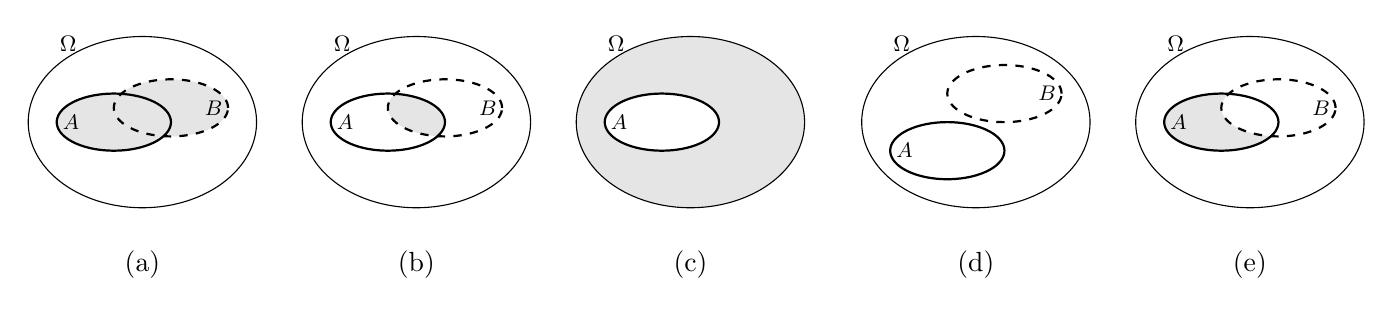
\begin{tikzpicture}[scale=.725]
\shorthandoff{>}
%
% Union y interseccion:
%
% Omega: .25*(x-.25)^2 + (y/1.5)^2 = 1
% A: x^2 + 4 y^2 = 1
% B: (x-1)^2 + 4 (y-1/4)^2 = 1
% A y B se cruzan cuando x = 1 \pm sqrt(55)/10 =>
% theta = acos(.5 \pm sqrt(55)/20) para A
% theta = acos(-.5 \pm sqrt(55)/20) para A
\pgfmathsetmacro{\s}{acos(.5-sqrt(55)/20)};
\pgfmathsetmacro{\t}{-acos(.5+sqrt(55)/20)};
\pgfmathsetmacro{\u}{-acos(-.5+sqrt(55)/20)};
\pgfmathsetmacro{\v}{acos(-.5-sqrt(55)/20)-360};
%
%
%Union
\begin{scope}
%
\fill[opacity=.1]
plot[domain=\s:\t+360,samples=200] ({cos(\x)},{.5*sin(\x)})
-- plot[domain=\u:\v+360,samples=200] ({cos(\x)+1},{.5*sin(\x)+.25})
-- cycle;
%
% borders A, B y Omega
\draw[domain=0:360,samples=200,thick] plot ({cos(\x)},{.5*sin(\x)});
\draw[dashed,domain=0:360,samples=200,thick] plot ({cos(\x)+1},{.5*sin(\x)+.25});
\draw[domain=0:360,samples=200] plot ({2*cos(\x)+.5},{1.5*sin(\x)});
%
% A, B, Omega
\draw (-.75,0) node[scale=.85]{\small $A$};
\draw(1.75,.25) node[scale=.85]{\small $B$};
\draw(-.5,1.375) node[left,scale=.9]{\small $\Omega$};
%
\draw (.5,-2.5) node{(a)};
\end{scope}
%
%
% Interseccion
\begin{scope}[xshift=4.8cm]
%
\fill[opacity=.1]
plot[domain=\s:\t,samples=200] ({cos(\x)},{.5*sin(\x)})
-- plot[domain=\u:\v,samples=200] ({cos(\x)+1},{.5*sin(\x)+.25})
-- cycle;
%
% borders A, B y Omega
\draw[domain=0:360,samples=200,thick] plot ({cos(\x)},{.5*sin(\x)});
\draw[dashed,domain=0:360,samples=200,thick] plot ({cos(\x)+1},{.5*sin(\x)+.25});
\draw[domain=0:360,samples=200] plot ({2*cos(\x)+.5},{1.5*sin(\x)});
%
% A, B, Omega
\draw (-.75,0) node[scale=.85]{\small $A$};
\draw(1.75,.25) node[scale=.85]{\small $B$};
\draw(-.5,1.375) node[left,scale=.9]{\small $\Omega$};
%
\draw (.5,-2.5) node{(b)};
\end{scope}
%
%
% Complemento
\begin{scope}[xshift=9.6cm]
%
\fill[opacity=.1]
plot[domain=0:360,samples=200] ({2*cos(\x)+.5},{1.5*sin(\x)})
-- plot[domain=0:360,samples=200] ({cos(\x)},{-.5*sin(\x)})
-- cycle;
%
% borders A y Omega
\draw[domain=0:360,samples=200,thick] plot ({cos(\x)},{.5*sin(\x)});
\draw[domain=0:360,samples=200] plot ({2*cos(\x)+.5},{1.5*sin(\x)});
%
% A, Omega
\draw (-.75,0) node[scale=.85]{\small $A$};
\draw(-.5,1.375) node[left,scale=.9]{\small $\Omega$};
%
\draw (.5,-2.5) node{(c)};
\end{scope}
%
%
% Excluyentes
\begin{scope}[xshift=14.6cm]
%
% borders A, B (con un shift...) y Omega
\draw[domain=0:360,samples=200,thick] plot ({cos(\x)},{.5*sin(\x)-.5});
\draw[dashed,domain=0:360,samples=200,thick] plot ({cos(\x)+1},{.5*sin(\x)+.5});
\draw[domain=0:360,samples=200] plot ({2*cos(\x)+.5},{1.5*sin(\x)});
%
% A, B, Omega
\draw (-.75,-.5) node[scale=.85]{\small $A$};
\draw (1.75,.5) node[scale=.85]{\small $B$};
\draw(-.5,1.375) node[left,scale=.9]{\small $\Omega$};
%
\draw (.5,-2.5) node{(d)};
\end{scope}
%
%
% privado
\begin{scope}[xshift=19.4cm]
%
\fill[opacity=.1]
plot[domain=\s:\t+360,samples=200] ({cos(\x)},{.5*sin(\x)})
-- plot[domain=\u:\v,samples=200] ({cos(\x)+1},{.5*sin(\x)+.25})
-- cycle;
%
% borders A, B y Omega
\draw[domain=0:360,samples=200,thick] plot ({cos(\x)},{.5*sin(\x)});
\draw[dashed,domain=0:360,samples=200,thick] plot ({cos(\x)+1},{.5*sin(\x)+.25});
\draw[domain=0:360,samples=200] plot ({2*cos(\x)+.5},{1.5*sin(\x)});
%
% A, B, Omega
\draw (-.75,0) node[scale=.85]{\small $A$};
\draw(1.75,.25) node[scale=.85]{\small $B$};
\draw(-.5,1.375) node[left,scale=.9]{\small $\Omega$};
%
\draw (.5,-2.5) node{(e)};
\end{scope}
%
\end{tikzpicture} \end{center}
%
\leyenda{Ilustraci\'on de las operaciones entre eventos: (a)~uni\'on $A \cup B$,
  (b)~intersecci\'on   $A  \cap   B$,  (c)~complemento   $\bar{A}$,  (d)~eventos
  excluyentes  $A  \cap  B  =  \emptyset$,  \ y  (e)~$A  \setminus  B$.  $A$  es
  representado en l\'inea  llena, $B$ en l\'inea discontinua;  en (a)-(c) y (e),
  el resultado de la operaci\'on es la zona sombreada.}
\label{Fig:MP:Ensembles}
\end{figure}

Formalmente, se define  de manera abstracta un espacio  medible $(\Omega,\A)$ de
la  manera siguiente  (~\cite{Hal50,  Fel68, Fel71,  Bre88, IbaPar97,  AthLah06,
  Bog07:v1, Coh13}; ver  tambi\'en~\cite[\& Ref.]{BarNov78, Bor98, Sie18, Sie75,
  Sie76} para notas hist\'oricas):
%
\begin{definicion}[Espacio medible]
\label{Def:MP:EspacioMedible}
%
  $(\Omega,  \A)$,  \  formado por  un  espacio  muestral  \  $\Omega$ \  y  una
  colecci\'on \  $\A$ \ de  conjuntos de \  $\Omega$, \ es llamado  {\it espacio
    medible} si satisface los requisitos
  %
  \begin{enumerate}
  \item $\emptyset \in \A$,
  %
  \item si $A \in \A$, entonces \ $\bar{A} \in \A$,
  %
  \item la uni\'on numerable de conjuntos de $\A$ queda en $\A$ ($\A$ es cerrado
    por la uni\'on numerable).
  %
  \end{enumerate}
  %
  Con  estas propiedades,  $\A$  es llamada  una  {\it $\sigma$-\'algebra}.  Los
  elementos de $\A$ son dichos {\it medibles}.
\end{definicion}
%
\noindent Es sencillo mostrar que $\Omega$  tambi\'en est\'a en $\A$, y que $\A$
es cerrado  por la intersecci\'on  numerable.  Un ejemplo  de $\sigma$-\'algebra
sobre \ $\Omega = \{ 1 \,  , \, 2 \, , \, 3 \, , \, 4 \, ,  \, 5 \, , \, 6 \}$ \
puede ser \ $\A = \big\{ \emptyset \, , \, \Omega \, , \, \{ 1 \, , \, 2 \, , \,
3 \} \, , \, \{ 4 \, , \, 5 \, , \, 6 \} \big\}$.

A partir de \ $(\Omega,\A)$, \ se  asocia una noci\'on de probabilidad \ $P$ \ a
un dado  evento. Esta queda  determinada por los siguientes  requisitos llamados
{\it  Axiomas  de Kolmogorov}  (ver  por  ejemplo~\cite{Spi76, Kol56,  ShaVov06,
  Pla05}):
%
\begin{enumerate}
\item $P(A) \geq 0 \ \ \forall \ A \in \A$.
%
\item Si  $A_1 , \ldots  , A_i ,  \ldots$ son eventos mutuamente  excluyentes de
  $\A$, entonces $\displaystyle P\left( \bigcup_i A_i \right) = \sum_i P(A_i)$.
%
\item $P(\Omega) = 1$.
\end{enumerate}
%
M\'as formalmente,  se define  un {\it espacio  de probabilidad} o  {\it espacio
  probabil\'istico}  de la  manera siguiente~\cite{Hal50,  Fel68,  Fel71, Bre88,
  IbaPar97, AthLah06, Bog07:v1, JacPro03, Coh13}:
%
\begin{definicion}[Espacio de medida y espacio probabil\'istico]
\label{Def:MP:EspacioProbabilistico}
%
  Sea $(\Omega,\A)$ un espacio medible.  Una funci\'on $\mu: \A \mapsto \Rset_+$
  tal que
  %
  \begin{enumerate}
  \item $\mu(\emptyset) = 0$, y
  \item para cualquier conjunto numerable  $\{ A_i \}_{i \in I}$ ($I$ numerable)
    de elementos  mutuamente excluyentes de  $\A$ se tiene  $\mu\left( \bigcup_i
      A_i \right) = \sum_i \mu(A_i)$,
  \end{enumerate}
  %
  es  llamada {\it  funci\'on  medida}  o {\it  medida  $\sigma$-aditiva}, y  el
  espacio $(\Omega,\A,\mu)$ es llamado {\it espacio de medida}.
  %
  \begin{itemize}
  \item Cuando \ $\mu$ \ es tal que existe un conjunto numerable \ $\{ A_i \}_{i
      \in I}$  \ ($I$ numerable) de  elementos de \ $\A$  \ tal que  \ $\Omega =
    \cup_{i \in I} A_i$  \ y \ $\forall \: i \in I,  \quad \mu(A_i) < +\infty$ \
    finito, la  medida se dice {\it  $\sigma$-finita} y el espacio  de medida se
    dice $\sigma$-finito.
  %
  \item Cuando $\mu$ est\'a acotada por  arriba, $\mu(\Omega) < + \infty$, la medida
    se dice {\it finita} y el espacio de medida tambi\'en se dice finito.
  %
  \item Adem\'as,  si \  $\mu(\Omega) = 1$,  la medida  es dicha medida  de {\it
      probabilidad}. En general,  se la denota \ $P$.  En  este caso, el espacio
    $(\Omega,\A,P)$ es llamado {\it espacio probabil\'istico}.
\end{itemize}
\end{definicion}
%
\noindent (ver tambi\'en~\cite[Cap.~5 \&  6]{KolFom61}). Es importante notar que
una combinaci\'on lineal positiva de medidas  es una medida, pero el producto de
dos medidas no es una medida m\'as.

A  partir de  los axiomas  de Kolmogorov  se pueden  probar varios  corolarios y
propiedades:
%
\begin{itemize}
\item la probabilidad de un evento seguro o cierto es 1;
%
\item la  probabilidad de un evento  que no puede  ocurrir es 0: \  por ejemplo,
  $P(\emptyset) = 0$;
%
\item el rango  de las probabilidades est\'a  acotado: \ $0 \leq P(A)  \leq 1\ \
  \forall \ A \in \A$;
%
\item condici\'on de  normalizaci\'on: \ si $\Omega =  \bigcup_{i=1}^n A_i$, con
  $A_i$  mutuamente  excluyentes,  entonces  \  $\sum_{i=1}^n P(A_i)  =  1$;  el
  conjunto  $\{  A_i \}_{i=1}^n$  se  dice  {\it  conjunto completo  de  eventos
    posibles    excluyentes    entre    s\'i}    y   es    ilustrado    en    la
  Figura~\ref{Fig:MP:CompletoSub};
%
\item si $A$ es subconjunto de $B$,  lo que escribiremos $A \subset B$, es decir
  que si  $B$ se realiza,  $A$ se realiza  tambi\'en (pero no  necesariamente al
  rev\'es),   entonces    \   $P(A)   \leq    P(B)$;   es   ilustrado    en   la
  Figura~\ref{Fig:MP:CompletoSub}.
\end{itemize}

\begin{figure}[h!]
\begin{center} 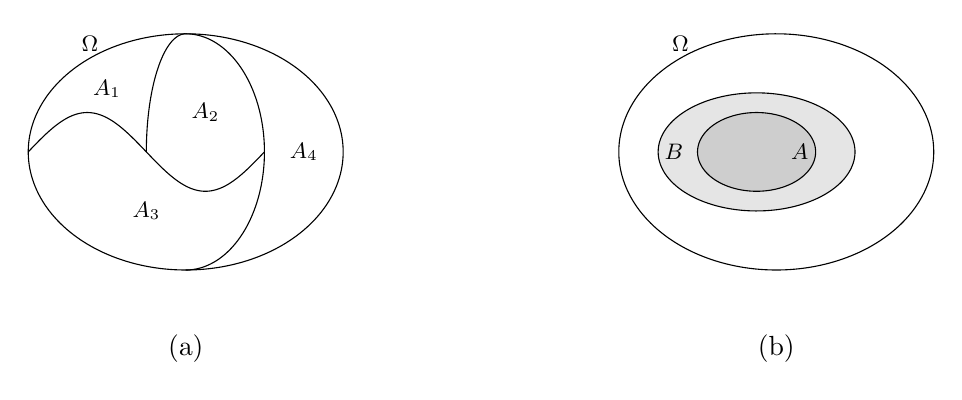
\begin{tikzpicture}%[scale=.9]
\shorthandoff{>}
%
% Particion
\begin{scope}
%
% Omega y A_i
\draw[domain=0:360,samples=200] plot ({2*cos(\x)+.5},{1.5*sin(\x)});
\draw[domain=-90:90,samples=200] plot ({cos(\x)+.5},{1.5*sin(\x)});
\draw[domain=90:180,samples=200] plot ({.5*cos(\x)+.5},{1.5*sin(\x)});
\draw[domain=0:3,samples=200] plot (\x-1.5,{.5*sin(120*\x)});
%
%
% Omega y A_i's
\draw(-.5,1.375) node[left,scale=.9]{\small $\Omega$};
\draw(-.5,.8) node[scale=.9]{\small $A_1$};
\draw(.75,.5) node[scale=.9]{\small $A_2$};
\draw(0,-.75) node[scale=.9]{\small $A_3$};
\draw(2,0) node[scale=.9]{\small $A_4$};
%
\draw (.5,-2.5) node{(a)};
\end{scope}
%
%
% Inclusion
\begin{scope}[xshift=7.5cm]
%
\fill[opacity=.1] plot[domain=0:360,samples=200] ({1.25*cos(\x)+.25},{.75*sin(\x)});
\fill[opacity=.1] plot[domain=0:360,samples=200] ({.75*cos(\x)+.25},{.5*sin(\x)});
%
% borders A, B y Omega
\draw[domain=0:360,samples=200] plot ({1.25*cos(\x)+.25},{.75*sin(\x)});
\draw[domain=0:360,samples=200] plot ({.75*cos(\x)+.25},{.5*sin(\x)});
\draw[domain=0:360,samples=200] plot ({2*cos(\x)+.5},{1.5*sin(\x)});
%
% A, B, Omega
\draw(.8,0) node[scale=.9]{\small $A$};
\draw (-.8,0) node[scale=.9]{\small $B$};
\draw(-.5,1.375) node[left,scale=.9]{\small $\Omega$};
%
\draw (.5,-2.5) node{(b)};
\end{scope}
%
\end{tikzpicture} \end{center}
%
\leyenda{Ilustraci\'on de: (a) conjunto completo de eventos posibles excluyentes
  entre s\'i;  (b) inclusi\'on  entre eventos, donde  $A$ est\'a en  gris oscuro
  mientras que $B$ est\'a en gris (claro y oscuro).}
\label{Fig:MP:CompletoSub}
\end{figure}

La probabilidad  \ $P(A \cap B)$  \ del evento $A  \cap B$ \  se llama tambi\'en
{\it probabilidad conjunta} de \ $A$ \ y \ $B$.  Se demuestra que
%
\begin{itemize}
\item $P(A  \cap B)$ est\'a acotada:  \ $0 \leq P(A  \cap B) \leq  \min\{ P(A) ,
  P(B)\}$ \ (viene de \ $A \cap B \subset A$ \ y \ $A \cap B \subset B$);
%
\item si $A$  y $B$ son mutuamente excluyentes,  entonces \ $P(A \cap B)  = 0$ \
  (viene de \ $A \cap B = \emptyset$);
%
\item  si  $\{ B_j  \}_{j=1}^m$  es un  conjunto  completo  de eventos  posibles
  excluyentes  entre s\'i,  entonces \  $\sum_{j=1}^m P(A  \cap B_j)  =  P(A)$ \
  (viene de $\{ A \cap B_j  \}_j$ mutuamente excluyentes y \ $\bigcup_j \left( A
    \cap B_j\right) = A \cap \left( \bigcup_j B_j \right) = A \cap \Omega = A$).
\end{itemize}

En el caso de eventos no necesariamente mutuamente excluyentes, se prueba que la
{\it ley de composici\'on} o {\it f\'ormula de inclusi\'on-exclusi\'on} es
%
\[
P(A \cup B) = P(A) + P(B) - P(A \cap B) \leq P(A) + P(B), 
\]
%
y que para $n$ eventos resulta
%
\[
P\left( \bigcup_{i=1}^n A_i \right) \leq \sum_{i=1}^n P\left( A_i \right).
\]
%
La  igualdad  vale  en  el  caso  especial  de  eventos  mutuamente  excluyentes
(recuperando el segundo axioma de Kolmogorov).

Se prueba tambi\'en  que si $\{ A_i \}_{i = 1}^{+\infty}$  es una secuencia {\it
  creciente} de  eventos, \ie $\forall \,  i \ge 1, \quad  A_i \subset A_{i+1}$,
entonces
%
\[
P\left( \bigcup_{i=1}^{+\infty} A_i \right) = \lim_{i \to +\infty} P(A_i).
\]
%
Por otro lado, si $\{ A_i \}_{i=1}^{+\infty}$ es una secuencia {\it decreciente}
de eventos, \ie $\forall \, i \ge 1, \quad A_{i+1} \subset A_i$, entonces
%
\[
P\left( \bigcap_{i=1}^{+\infty} A_i \right) = \lim_{i \to +\infty} P(A_i).
\]

Podemos preguntarnos cu\'al es la probabilidad  de un evento $A$, si sabemos que
se da  cierto evento~$B$.   Por ejemplo,  para un dado  de 6  caras equilibrado,
cu\'al  es la  probabilidad de  tener un  n\'umero par  sabiendo que  tenemos un
n\'umero menor o  igual a 3.  La  respuesta se encuentra en la  noci\'on de {\it
  probabilidad   condicional}~\cite{Hau01,   Jef48,   Jef73,  Bre88,   ManWol95,
  JacPro03, ShaVov06}:
%
\begin{definicion}[Probabilidad condicional]
\label{Def:MP:ProbaCondicional}
%
  La  {\it probabilidad  condicional} de  $A$  dado $B$,  denotado $P(A|B)$,  se
  define  como  la  raz\'on entre  la  probabilidad  del  evento conjunto  y  la
  probabilidad de que se d\'e $B$ (cuando \'este es un evento de probabilidad no
  nula):
  %
  \[
  P(A|B) = \frac{P(A \cap B)}{P(B)}.
  \]
\end{definicion}
%
En  el  ejemplo precedente,  la  probabilidad condicional  va  a  ser $P(A|B)  =
\frac{P(A \cup B)}{P(B)} = \frac{\frac16}{\frac12} = \frac13$.

Claramente  del  hecho  de  que  \  $P$  \ es  una  medida  de  probabilidad  se
tiene \[P(A|B) \ge 0.\] Luego, de \ $A \cap B \subseteq B$ \ resulta \ $P(A \cap
B) \le  P(B)$; es decir,  \[ P(A|B) \le  1. \] Adem\'as,  \ $P(\Omega \cap  B) =
P(B)$ \ dando  \[P(\Omega|B) = 1.\] Para  cualquier conjunto \ $\{ A_i  \}$ \ de
eventos  mutuamente  excluyentes,  los \  $\left(  A_i  \cap  B \right)$  \  son
tambi\'en  mutuamente excluyentes,  as\'i  que \  $\displaystyle P\left(  \left(
    \bigcup_i  A_i \right)  \bigcap B  \right)  = P\left(  \bigcup_i \left(  A_i
    \bigcap  B  \right)  \right) =  \sum_i  P\left(  A_i  \bigcap B  \right)$  \
dando \[P\left( \left.  \bigcup_i A_i  \right| B \right) = \sum_i P\left( \left.
    A_i \right|  B \right).\] Dicho  de otra manera,  $P(A|B)$ es una  medida de
probabilidad~\footnote{Se puede definir un  espacio de probabilidad $( \Omega_B,
  \A_B  , P_B)$  donde  $P_B(A)  \equiv P(A|B)$.  La  notaci\'on $P_B(A)$  suele
  utilizarse  en  la  literatura pero  no  la  usaremos  en  esta obra  para  no
  confundirla  con la  medida  de  probabilidad de  una  variable aleatoria  que
  definiremos   en   la   secci\'on   siguiente.}.   Diversas   situaciones   de
probabilidades condicionales son ilustradas en la Fig.~\ref{Fig:MP:Condicional}.

\begin{figure}[h!]
\begin{center} 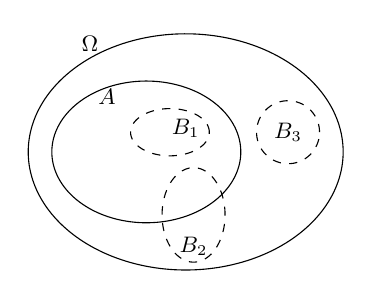
\begin{tikzpicture}%[scale=.9]
\shorthandoff{>}
%
\begin{scope}
%
% Omega, A, B_i
\draw[domain=0:360,samples=200] plot ({2*cos(\x)+.5},{1.5*sin(\x)});
\draw[domain=0:360,samples=200] plot ({1.2*cos(\x)},{.9*sin(\x)});
\draw[dashed,domain=0:360,samples=200] plot ({.5*cos(\x)+.3},{.3*sin(\x)+.25});
\draw[dashed,domain=0:360,samples=200] plot ({.4*cos(\x)+.6},{.6*sin(\x)-.8});
\draw[dashed,domain=0:360,samples=200] plot ({.4*cos(\x)+1.8},{.4*sin(\x)+.25});
%
%
% Omega y A_i's
\draw(-.5,1.375) node[left,scale=.9]{\small $\Omega$};
\draw(-.5,.7) node[scale=.9]{\small $A$};
\draw(.5,.3) node[scale=.9]{\small $B_1$};
\draw(.6,-1.2) node[scale=.9]{\small $B_2$};
\draw(1.8,.25) node[scale=.9]{\small $B_3$};
%
\end{scope}
%
\end{tikzpicture} \end{center}
%
\leyenda{Ilustraci\'on  de la probabilidad  condicional con  $A$ interior  de la
  curva  en l\'inea  llena y  unos $B_i$  interiores de  las curvas  en l\'ineas
  discontinuas. Se tiene \ $\omega \in B_1 \Rightarrow \omega \in A$ \ as\'i que
  \ $P(A|B_1) = 1$; por otro  lado, \ $\omega \in B_3 \Rightarrow \omega \not\in
  A$  \ as\'i  que  \ $P(A|B_3)  =  0$.  Entre  estas  situaciones extremas,  si
  $P(\bar{A}  \cap B_2)  \ne 0$  \ y  \ $P(A  \cap B_2)  \ne 0$  \ tenemos  $0 <
  P(A|B_2) < 1$ (se puede tomar el ejemplo de probabilidad de un evento iguale a
  su superficia  sobre la de  $\Omega$ para ver  estas propiedades en  este caso
  particular).}
\label{Fig:MP:Condicional}
\end{figure}

Algunas propiedades interesantes son las siguientes:
%
\begin{itemize}
\item $P(A \cap B | B) = P(A|B)$ \  \big(viene de $P(A \cap B \cap B) = P(A \cap
  B)$\big);
%
\item si $A$ \ y \ $B$ \ son mutuamente excluyentes, obviamente \ $P(A|B) = 0$;
%
\item si $B \subseteq C$, entonces \ $P(A  | B \cap C) = P(A|B)$ \ \big(viene de
  \ $P(A | B  \cap C) = \frac{P(A \cap B \cap C)}{P(B  \cap C)} = \frac{P(A \cap
    B)}{P(B)}$, \ pues\ $B \cap C = B$\big);
%
\item  condici\'on de  normalizaci\'on:  \ si  \  $\{ A_i  \}_{i=1}^n$  \ es  un
  conjunto completo  de resultados  posibles mutuamente excluyentes,  entonces \
  $\sum_{i=1}^n P(A_i|B) = 1$;
%
\item relaci\'on  entre probabilidades condicionales  inversas: \ $\displaystyle
  P(B|A)  = \frac{P(B)}{P(A)}  P(A|B)$, de  donde \  $P(A|B)$ \  y \  $P(B|A)$ \
  coinciden s\'olo cuando \ $A$ \ y \ $B$ \ tienen la misma probabilidad;
%
\item {\it  f\'ormula de probabilidad  total}: \ si  $\{ B_j \}$ es  un conjunto
  completo de eventos no nulos mutuamente excluyentes, entonces
  %
  \[
  P(A) = \sum_j P(A|B_j) P(B_j) 
  \]
  %
  \big(viene de \ $A = A \cap  \left( \bigcup_j B_j \right) = \bigcup_j \left( A
    \cap B_j \right)$ \ donde los \ $A \cap B_j$ \ son mutuamente excluyentes, y
  $P\left( A \cap B_j \right) = P(A|B_j) P(B_j)$\big) ;
%
\item {\it  f\'ormula de Bayes}:  \ si  $\{ B_j \}$  es un conjunto  completo de
  eventos no nulos mutuamente excluyentes, entonces
  %
  \[
  P(B_i|A) = \frac{P(A \cap B_i)}{P(A)} = \frac{P(A|B_i) P(B_i)}{\sum_j P(A|B_j)
    P(B_j)};
  \]
  %
  (ver~\cite{Bre88, JacPro03, Bay63, Bar58}~\footnote{La obra del matem\'atico y
    religioso  ingl\'es  Thomas  Bayes  fue  de  hecho  recopilada  y  publicada
    despu\'es de su muerte por Richard Price.} ).
\end{itemize}

Veamos ahora la noci\'on de independencia  entre dos eventos. Por ejemplo, si se
tiran dos dados  sobre sendas mesas, no hay ninguna raz\'on  para que la muestra
de  uno  ``influya''  la  del  otro.  Dicho de  otra  manera,  dos  eventos  son
independientes  si el  conocimiento de  uno no  lleva  ninguna ``informaci\'on''
sobre el otro~\cite{Bre88, ManWol95, Hau01, JacPro03, Bor09}:
%
\begin{definicion}[Independencia estad\'istica]
\label{Def:MP:IndependenciaEtadistica}
%
  Dos eventos \ $A$ \ y \ $B$ \ se dicen {\it estad\'isticamente independientes}
  si la  probabilidad condicional  de $A$  dado $B$ es  igual a  la probabilidad
  incondicional de $A$:
  %
  \[
   P(A|B) = P(A).
   \]
  %
   Es equivalente al hecho de que la probabilidad conjunta se factoriza: 
  %
  \[
   P(A \cap B) = P(A) P(B).
   \]
\end{definicion}
%
Por  inducci\'on, la  condici\'on necesaria  y suficiente  para que  $n$ eventos
$A_1,\ldots,A_n$  sean mutuamente  estad\'isticamente independientes  es  que la
probabilidad conjunta se factorice como
%
\[
P\left( \bigcap_{i=1}^n A_i \right) = \prod_{i=1}^n P(A_i).
\]
%
Se  deduce que  los  eventos mutuamente  excluyentes  no son  estad\'isticamente
independientes.

Es  importante  notar  que  la  independencia  mutua  no  es  equivalente  a  la
independencia por pares de eventos, como lo ilustra el ejemplo siguiente.
%
\begin{ejemplo}[Independencia   mutua   vs    por   pares]
\label{Ej:MP:IndependenciaMutuaVsPares}
%
  Tiramos 2 dados independientemente y consideramos  los eventos: \ $A_i, i = 1,
  2$ \ ``el  dado $i$ es par'' y  $A_3$ ``la suma de ambos dados  es impar''. Es
  claro que \ $A_1$  \ y \ $A_2$ \ son independientes y adem\'as  para $i = 1$ o
  2, \ $P(A_i \cap A_3) = \frac14 = P(A_i) P(A_3)$, \ mientras que \ $P(A_1 \cap
  A_2 \cap A_3) = 0 \ne \frac18$: los eventos son independientes por pares, pero
  no son mutuamente independientes~\cite{HogMck13}.
\end{ejemplo}

\begin{definicion}[Independencia condicional]
\label{Def:MP:IndependenciaCondicional}
%
  Dos eventos \ $A$ \ y  \ $B$ \ se dicen {\it estad\'isticamente independientes
    condicionalmente} a un tercer evento  $C$, si la probabilidad conjunta de \
  $A$  \ y  \ $B$  \ condicionalmente  a  \ $C$  \ es  igual al  producto de  la
  probabilidad de  $A$ condicionalmente a $C$  por la de  $B$ condicionalmente a
  $C$:
  %
  \[
   P(A \cap B | C) = P(A | C) P(B |C).
   \]
   %
   Si $P(B|C) \ne 0$, es equivalente a $P(A|B \cap C) = P(A|C)$.
\end{definicion}
%
Es importante  notar  que dos  eventos pueden ser independientes,  pero no serlo
condicionalmente a un tercero, como lo ilustra el ejemplo siguiente.
%
\begin{ejemplo}[Independencia  incondicional pero  no condicional]
\label{Ej:MP:IndependenciaIncondicional}
%
  Teniendo dos monedas bien equilibradas y tir\'andolas de manera independiente,
  consideramos  los eventos  \ $A$  ``la  primera faz  es una  cruz'', $B$  ``la
  segunda faz  es una  cara'', $C$ ``las  faces son id\'enticas''.  Claramente \
  $P(A \cap B) = \frac14 = P(A) P(B)$, \ mientras que \ $P(A \cap B | C) = 0 \ne
  P(A|C) P(B|C) = \frac1{16}$.
\end{ejemplo}

Al rev\'es, dos eventos pueden ser condicionalmente independientes a un tercero,
pero  ser  dependientes.
%
\begin{ejemplo}[Independencia  condicional  pero  no  incondicional]
\label{Ej:MP:IndependenciaCondicional}
%
  Sea Alice tirando una moneda bien  equilibrada y denotamos $A$ el evento ``era
  una cruz''.   Claramente $P(A) =  \frac12$.  Suponemos que Alice  transmite el
  resultado a  Bob a trav\'es de  un intermediario Charlie  con una probabilidad
  $\varepsilon$ de  mentir a Charlie,  y llamamos $C$  el evento ``Alice  dijo a
  Charlie   que  era  una   cruz''.   Tenemos   que  $P(C)   =  P(C|A)   P(A)  +
  P(C|\widebar{A})  P(\widebar{A})  =   (1-\varepsilon)  \frac12  +  \varepsilon
  \frac12 =  \frac12$.  Suponemos ahora  que Charlie transmite  a Bob lo  que le
  dijo Alice, con una  probabilidad $\vartheta$ de mentir (independientemente de
  Alice) y llamamos $B$ el evento ``Charlie dijo a Bob que era una cruz''. Es de
  nuevo sencillo ver  que $P(B) = \frac12$.  Ahora, $P(A \cap  B |C) = \frac{P(A
    \cap B \cap C)}{P(C)} = 2 \, P(A \cap B \cap C)$. El evento \ $A \cap B \cap
  C$ \ es  era una cruz y Alice  no mint\'o y Charlie tampoco, es  decir, por la
  independencia:    $P(A   \cap    B   |C)    =   (1-\varepsilon)(1-\vartheta)$.
  Inmediatamente $P(B|C)  = 1-\vartheta$ \  y \  $P(A|C) = 2  \, P(A \cap  C)$ \
  siendo  \ $A  \cap  C$ \  el  evento ``era  una cruz  y  Alice no  minti\'o'',
  i.e. $P(A|C)  = 1-\varepsilon$. En  conclusi\'on, \ $P(A  \cap B |C)  = P(A|C)
  P(B|C)$: $A$  y $B$  son independientes condicionalmente  a $C$.   Ahora, $P(A
  \cap  B) =  P(A \cap  B  \cap C)  + P(A  \cap  B \cap  \widebar{C}) =  \frac12
  (1-\varepsilon)(1-\vartheta)  + \frac12  \varepsilon \vartheta  \ne  \frac14 =
  P(A) P(B)$ en  general: $A$ y $B$ no resultan  independientes. Este ejemplo es
  una instancia de lo que se llama un proceso de Markov, que vamos a ver un poco
  m\'as en el c\'apitulo~\ref{Cap:SZ:Informacion}.
\end{ejemplo}


% ============ Variables aleatorias y distribuciones de probabilidad =========== %

\seccion{Variables aleatorias y distribuciones de probabilidad}
\label{Sec:MP:variablealeatoria}

En un experimento  o un dado proceso, los  posibles resultados son t\'ipicamente
n\'umeros  reales, siendo  cada n\'umero  un evento.   Luego los  resultados son
mutuamente  excluyentes. Se  considera  a  esos n\'umeros  como  valores de  una
\emph{variable aleatoria} $X$ a valores reales, que puede ser discreta, continua
o mixta.

Formalmente, la  noci\'on de  variable aleatoria se  apoya sobre la  noci\'on de
funci\'on  medible.  Por  esta  formalizaci\'on, vamos  a  necesitar definir  la
integraci\'on de  manera general,  m\'as all\'a del  enfoque de Riemann  (``a la
Lebesgue''), as\'i  como la noci\'on  de derivada de  una medida con  respecto a
otra para  definir densidades  de probabilidad, en  analog\'ia a la  densidad de
masa en mec\'anica por ejemplo~\cite{Leb04, Leb18, KolFom61, AthLah06, Bog07:v1,
  Coh13}.


% ================================= Medida, integral, densidades

\subseccion{Consideraciones  preliminaries:  Teor\'ias  de  la medida  y  de  la
  integraci\'on.}
\label{Ssec:MP:VAPreliminaria}

La primera noci\'on  que subyace a la definici\'on  formal de variable aleatoria
es la de funci\'on medible:

\begin{definicion}[Funci\'on medible]
\label{Def:MP:FuncionMedible}
%
 Sean  \ $(\Omega,\A)$  \ y  \ $(\Upsilon,\B)$  \ dos  espacios  medibles.  Una
  funci\'on $f: \Omega \mapsto \Upsilon$ se dice {\it $(\A,\B)$-medible} si
  %
  \[
  \forall \,  B \in  \B, \quad  A \equiv f^{-1}(B)  = \left\{  \omega \in  A \tq
    f(\omega) \in B \right\} \: \in \: \A.
  \]
  %
  Dicho de  otra manera, la pre-im\'agen  de un elemento dado  de $\B$ (elemento
  medible) pertenece a $\A$ (elemento medible).  Por abuso de escritura, se dice
  m\'as simplemente que $f: (\Omega,\A) \mapsto (\Upsilon,\B)$ es medible.
\end{definicion}

Adem\'as, a partir de un espacio de medida y una funci\'on $f$ medible, se puede
definir  una  medida  im\'agen   sobre  el  espacio  de  llegada~\cite{AthLah06,
  Bog07:v1, Coh13}:
%
\begin{teorema}[Teorema de la medida im\'agen]
\label{Teo:MP:MedidaImagen}
%
  Sean  \ $(\Omega,\A,\mu)$  \  un espacio  de  medida, \  $(\Upsilon,\B)$ \  un
  espacio  medible  y  $f:  (\Omega,\A)  \mapsto  (\Upsilon,\B)$  una  funci\'on
  medible. Sea $\mu_f$ tal que
  %
  \[
  \forall \,  B \in  \B, \quad  \mu_f(B) = \mu\left( f^{-1}(B) \right).
  \]
  %
  Entonces, $\mu_f$  es una medida  sobre el espacio medible  $(\Upsilon,\B)$, \
  \ie  \  $(\Upsilon,\B,\mu_f)$  \  define  un  espacio  de  medida.   Adem\'as,
  $\mu(\Omega) = \mu_f(\Upsilon)$ (posiblemente  infinitas). Se dice que $\mu_f$
  es la {\it medida im\'agen de $\mu$ por $f$}.
\end{teorema}
%
\begin{proof}
  Por   definici\'on,  claramente   $\mu_f  \ge   0$.    Adem\'as,  obviosamente
  $f^{-1}(\emptyset) =  \emptyset$ \ dando $\mu_f(\emptyset)  = \mu(\emptyset) =
  0$.  Luego,  si para un  conjunto numerable $\{  B_j \}$ de elementos  de $\B$
  disjuntos entre s\'i, las pre-im\'agenes  de los $B_j$ tambi\'en son disjuntos
  entre s\'i  (para $k  \ne j$ no  se puede  tener $\omega \in  f^{-1}(B_j) \cap
  f^{-1}(B_k)$  sino  $\omega$  tendr\'ia  dos im\'agenes  distintas  por  $f$).
  Entonces \ $f^{-1}\left( \bigcup_j B_j \right) = \bigcup_j f^{-1}(B_j)$.  Esto
  implica  que \  $\mu_f\left( \bigcup_j  B_j \right)  =  \mu\left( f^{-1}\left(
      \bigcup_j B_j \right) \right)  = \mu\left( \bigcup_j f^{-1}(B_j) \right) =
  \sum_j  \mu\left(  f^{-1}(B_j)  \right)  =  \sum_j  \mu_f(B_j)$.   Finalmente,
  necesariamente  $f^{-1}(\Upsilon) =  \Omega$ (obviamente  $f(\Omega) \subseteq
  \Upsilon$)  lo  que  cierra  la  prueba~\footnote{De hecho,  se  puede  probar
    sencillamente que la pre-im\'agen de  una uni\'on numerable (disjuntos o no)
    es la uni\'on de las  pre-im\'agenes; lo mismo occure para la intersecci\'on
    y  adem\'as  la  pre-im\'agen  del  complemento  es  el  complemento  de  la
    pre-im\'agen.  Esto se conoce  como {\it leyes de de Morgan}~\cite{AthLah06,
      Coh13,        HogMck13}       (ver       tambi\'en~\cite[Cap.~1]{KolFom57}
    y~\cite[Caps.~5~\&~6]{KolFom61}).\label{Foot:MP:Jacobiana}}
\end{proof}

A  continuaci\'on,  necesitaremos  tratar  de funciones  medibles  teniendo  una
propiedad (P) salvo sobre  un conjunto de medida \ $\mu$ \  igual a cero.  M\'as
generalmente viene ac\'a la noci\'on de propiedad {\it casi siempre}:
%
\begin{definicion}[Propiedad (e igualdad) $\mu$-casi siempre]
\label{Def:MP:CasiSiempre}
%
  Una funcion  medible \  $f$ se  dice tener una  propiedad (P)  dada $\mu$-casi
  siempre, si y solamente si la tiene excepto sobre un conjunto de medida nula,
  %
  \[
  \mu\left( \left\{ \omega  \tq f(\omega) \: \mbox{ no  satisface (P) } \right\}
  \right) = 0.
  \]
  %
  Por ejemplo, dos funciones medibles \ $f_1$ \ y \ $f_2$ \ $(\Omega,\A,\mu) \to
  (\Upsilon,\B)$ \ son iguales $\mu$-casi siempre,
  \[
  f_1 = f_2 \quad (\mu\mbox{-c.s.})
  \]
  %
  si y solamente si son iguales excepto sobre un conjunto de medida nula,
  %
  \[
  \mu\left( \left\{ \omega \tq f_1(\omega) \ne f_2(\omega) \right\} \right) = 0.
  \]
\end{definicion}

\

Un espacio  que juega un rol particular  es $\Rset^d$, al cual  se puede asociar
una  $\sigma$-\'algebra  particular  conocida  como {\it  $\sigma$-\'algebra  de
  Borel}~\cite{AthLah06, Bog07:v1, Bog07:v2, Coh13}:
%
\begin{definicion}[$\Rset^d$ y Borelianos]
\label{Def:MP:Borelianos}
%
  Para  cualquier  $d  \ge  1$  entero,  llamamos  Borelianos  $\B(\Rset^d)$  de
  $\Rset^d$ a  la $\sigma$-\'algebra m\'as peque\~na generada  por los productos
  cartesianos     $\displaystyle    \optimes_{i=1}^d    (-\infty     \;    b_i]$
  \big(similarmente,  por  los  abiertos  de  $\Rset^d$, o  tambi\'en  para  los
  productos  cartesianos de intervalos  $\displaystyle \optimes_{i=1}^d  (a_i \;
  b_i]$\big), \ie uniones numerables, intersecciones numerables, complementos de
  estos intervalos.  $\B(\Rset^d)$  es tambi\'en llamado {\it $\sigma$-\'algebra
    de Borel de $\Rset^d$}.
\end{definicion}

\

Se necesita ahora definir la  noci\'on de integraci\'on de una funci\'on medible
con respecto a una medida:
%
\begin{definicion}[Medida e integraci\'on]
\label{Def:MP:MedidaIntegracion}
%
  Para una medida  cualquiera, sobre un espacio de  medida $(\Omega,\A,\mu)$, se
  define la integraci\'on a partir de
  %
  \[
  \forall \, A \in \A,  \quad \int_A d\mu(\omega) = \int_\Omega \un_A(\omega) \,
  d\mu(\omega) = \mu(A),
  \]
  %
  donde $\un_A$ es la funci\'on indicadora (ver notaciones).
  %
%  \[
%  \un_A(\omega) = \left\{
%  \begin{array}{ccc}
%  1 & \mbox{si} & \omega \in A\\
%  0 & \mbox{si} & \omega \not\in A
%  \end{array} \right.
%  \]
  %
  es  la funci\'on  indicadora del  conjunto $A$.   $d\mu(\omega)$ se  escribe a
  veces tambi\'en $\mu(d\omega)$,  medida de un ``infinit\'esimo''.  Claramente,
  por  propiedades  de una  medida,  para $  A_i,  A_j$  disjuntos $\un_{A_i}  +
  \un_{A_j}  =  \un_{A_i \cup  A_j}$,  dando  $\displaystyle \int_\Omega  \left(
    \un_{A_i} + \un_{A_j} \right) d\mu(\omega)  = \mu(A_i \cup A_j) = \mu(A_i) +
  \mu(A_j)  =   \int_\Omega  \un_{A_i}  d\mu(\omega)   +  \int_\Omega  \un_{A_j}
  d\mu(\omega)$ y entonces, sin perdida  de generalidad para un conjunto $\{ A_j
  \}$ numerable
  %, con los $A_j$ disjuntos,  
  y $\{  a_j \}$ reales no negativos,  la integral de la  funci\'on escalonada \
  $\displaystyle \sum_j a_j \un_{A_j}$ \ es dada por
  %
  \[
  \int_\Omega \left( \sum_j a_j \un_{A_j}(\omega) \right) \, d\mu(\omega) =
  \sum_j a_j \int_\Omega \un_{A_j}(\omega) \, d\mu(\omega).
  \]
  %
  Para  los  $A_i$  disjuntos  es   la  consecuencia  directa  de  la  propiedad
  precedente, y  si $A_i,  A_j$ no son  disjuntos.  De hecho,  sufice considerar
  $A_i\setminus A_j, \:  A_j\setminus A_i, A_i \cap A_j$ \ con  $A \setminus B =
  \{ \omega: \omega \in A \: \mbox{y} \: \omega \not\in B\}$ \ y respectivamente
  los  coefficientes \  $a_i, \:  a_j, \:  a_i  + a_j$  para volver  al caso  de
  conjuntos disjuntos.
  %
\end{definicion}


Antes de definir la integraci\'on de una funci\'on real, medible, cualquiera, el
\'ultimo paso que falta es el siguiente:
%
\begin{teorema}[Funci\'on medible como l\'imite]
\label{Teo:MP:MedibleLimite}
%
  Sea   \   $g:   (\Omega,\A)   \mapsto  (\Rset,\B(\Rset))$,   no   negativa   y
  medible. Existe  una sucesi\'on  \ $\{  g_n \}_{n \in  \Nset}$ \  creciente de
  funciones escalonadas que converge simplemente (punto a punto) hacia $g$.
\end{teorema}
%
\begin{proof}
  La  sucesi\'on \ $\displaystyle  g_n =  \sum_{k=0}^{n 2^n-1}  \frac{k}{2^n} \,
  \un_{g^{-1}\left( \left[ \frac{k}{2^n} \; \frac{k+1}{2^n} \right) \right)} + n
  \, \un_{g^{-1}\left(  \left[ n \;  +\infty \right) \right)}$ \  es escalonada,
  creciente y converge  hacia $g$ \ (notar que esta  sucesi\'on comparte la idea
  que subyace a la integraci\'on de Riemann).
\end{proof}

De  este resultado, se  puede generalizar  la noci\'on  de integraci\'on  de una
funci\'on real:
%
\begin{definicion}[Integraci\'on de una funci\'on real]
\label{Def:MP:IntegracionReal}
%
  Sea \ $g:  (\Omega,\A) \mapsto (\Rset,\B(\Rset))$, no negativa  y medible, y \
  $\{ g_n \}_{n \in \Nset}$  \ una sucesi\'on creciente de funciones escalonadas
  que converge simplemente hacia $g$. Por definici\'on,
  %
  \[
  \int_{\Omega}  g(\omega) \,  d\mu(\omega)  = \lim_{n  \to \infty}  \int_\Omega
  g_n(\omega) \, d\mu(\omega).
  \]
  %
  Notar  de  que  el  l\'imite  puede  ser infinita.\newline  Sea  ahora  \  $g:
  (\Omega,\A)  \mapsto  (\Rset,\B(\Rset))$ \  medible  cualquiera.  Se  verifica
  sencillamente  que  tambi\'en  $|g|$   (valor  absoluto)  es  medible  y,  por
  definici\'on, $g$ se dice $\mu$-integrable si la integral de $|g|$ es finita,
  %
  \[
  g   \:  \mbox{es}   \:  \mu\mbox{-integrable}   \quad   \Leftrightarrow  \quad
  \int_\Omega |g(\omega)| \, d\mu(\omega) < +\infty.
  \]
  %
  Adem\'as,  se  escribe $g  =  g_+  +  g_-$ con  $g_+  =  \max(g,0)$ y  $g_-  =
  \min(g,0)$. Es sencillo ver de que si \  $g$ \ es medible, \ $g_+$ \ y \ $g_-$
  \ son medibles. Si  \ $g$ \ es $\mu$-integrable, necesariamente \  $g_+$ \ y \
  $g_-$ \ son $\mu$-integrables, y, por definici\'on
  %
  \[
  \int_\Omega   g(\omega)   \,  d\mu(\omega)   =   \int_\Omega  g_+(\omega)   \,
  d\mu(\omega) - \int_\Omega \left( - g_-(\omega) \right) \, d\mu(\omega).
  \]
\end{definicion}

A continuaci\'on, damos  unos teoremas que ser\'an muy  \'utiles m\'as adelante,
sin detallar las pruebas. Por esto, el lector se puede referir a~\cite{LieLos01,
  AthLah06, Bog07:v1, Coh13}.
%
\begin{teorema}[Teorema de convergencia mon\'otona]
\label{Teo:MP:ConvergenciaMonotona}
%
  Sea  \ $\{  f_n \}_{n  \in  \Nset}$ \  una sucesi\'on  creciente de  funciones
  medibles  sobre $(\Omega,\A,\mu)$,  positivas, convergiendo  simplemente hacia
  una funci\'on \ $f$ \ medible. Entonces
  %
  \[
  \lim_{n  \to  +\infty}  \int_\Omega  f_n(\omega)  d\mu(\omega)  =  \int_\Omega
  f(\omega) d\mu(\omega).
  \]
\end{teorema}
%
De   hecho  se   prueba   este  teorema   a   partir  de   la  definici\'on   de
integraci\'on. Este  teorema da una condici\'on  simple permitiendo intercambiar
integraci\'on y l\'imite.

\begin{corolario}
\label{Cor:MP:ConvergenciaDominada}
%
  Sea \ $\{  f_n \}_{n \in \Nset}$ \ una sucesi\'on  de funciones medibles sobre
  $(\Omega,\A,\mu)$,  positivas,   tal  que  la  serie   $\sum_n  f_n$  converge
  simplemente hacia una funci\'on \ $f$, $\mu$-integrable. Entonces
  %
  \[
  \int_\Omega  \sum_{n   \in  \Nset}  f_n(\omega)   d\mu(\omega)  =  \int_\Omega
  f(\omega) d\mu(\omega).
  \]
\end{corolario}
%
Es  una consecuencia  del teorema  de convergencia  mon\'otona,  considerando la
sucesi\'on creciente $\{ \sum_{k=0}^n f_k \}_{n \in \Nset}$.

\begin{teorema}[Teorema de convergencia dominada]
\label{Teo:MP:ConvergenciaDominada}
%
  Sea  \ $\{  f_n \}_{n  \in  \Nset}$ \  una sucesi\'on  creciente de  funciones
  medibles sobre $(\Omega,\A,\mu)$  convergiendo simplemente hacia una funci\'on
  \ $f$, medible.  Suponemos que existe una funci\'on  $\mu$-integrable  \ $g$ \
  que  domina  la  sucesi\'on,  \ie  $\forall  \, \omega  \in  \Omega,  \quad  |
  f_n(\omega) | \le g(\omega)$. Entonces
  %
  \[
  \lim_{n  \to  +\infty}  \int_\Omega  f_n(\omega) \,  d\mu(\omega)  =  \int_\Omega
  f(\omega) \, d\mu(\omega) \le \int_\Omega  g(\omega)  \, d\mu(\omega).
  \]
\end{teorema}
%
Este  teorema  da  una  condici\'on  suficiente  muy \'util  y  muy  usada  para
asegurarse de que se puede intercambiar l\'imite e integraci\'on.

El   \'ultimo  teorema   que  vamos   a  necesitar   permite   intercambiar  dos
integraciones.   Antes,  necesitamos  definir  la noci\'on  de  espacio  medible
producto y medida producto.
%
\begin{definicion}[Espacio medible producto, medida producto]
\label{Def:MP:EspacioMedidaProductos}
%
  Sean dos  espacios de  medida \  $(\Omega_1, \A_1, \mu_1)$  \ y  \ $(\Omega_2,
  \A_2,  \mu_2)$. Llamamos  {\it espacio  medible producto}  $(\Omega ,  \A)$ al
  espacio del  producto cartesiano  $\Omega = \Omega_1  \times \Omega_2$  con la
  $\sigma$-\'algebra  $\A$ generada  por los  productos cartesianos  $A_1 \times
  A_2$ donde $A_i \in \A_i, i  = 1, 2$. Adem\'as, llamamos medida producto $\mu$
  definida sobre $\A$ a la medida  tal que $\forall \: (A_1,A_2) \in \A_1 \times
  \A_2, \quad \mu(A_1 \times A_2) = \mu_1(A_1) \mu_2(A_2)$.
\end{definicion}

\begin{teorema}[Teorema de Fubini]
\label{Teo:MP:Fubini}
%
  Sea  $(\Omega,\A,\mu)$  espacio de  medida  producto  de  \ $(\Omega_1,  \A_1,
  \mu_1)$ \  y \ $(\Omega_2,  \A_2, \mu_2)$ donde  $\mu$ es la  medida producto.
  Sea $f$ una funci\'on integrable sobre $(\Omega,\A,\mu)$ entonces 
  \begin{itemize}
  %
  \item  $\omega_1 \mapsto  f(\omega_1,\omega_2)$  \ es  \ $\mu_1$-integrable  \
    ($\mu_2$-c.s.)  \quad y \quad $\omega_2 \mapsto f(\omega_1,\omega_2)$ \ es \
    $\mu_2$-integrable \ ($\mu_1$-c.s.),
  %
  \item $\displaystyle \omega_1  \mapsto \int_{\Omega_2} f(\omega_1,\omega_2) \,
    d\mu_2(\omega_2)$  \ es  \ $\mu_1$-integrable  \quad y  \quad $\displaystyle
    \omega_2 \mapsto \int_{\Omega_1} f(\omega_1,\omega_2) \, d\mu_1(\omega_1)$ \
    es \ $\mu_2$-integrable.
  \end{itemize}
  %
  Adem\'as,
  %
  \[
  \int_{\Omega_1  \times \Omega_2}  f(\omega) \,  d\mu(\omega)  = \int_{\Omega_1}
  \left(    \int_{\Omega_2}   f(\omega)    \,   d\mu_2(\omega_2)    \right)   \,
  d\mu_1(\omega_1)   =  \int_{\Omega_2}   \left(  \int_{\Omega_1}   f(\omega)  \,
    d\mu_1(\omega_1) \right) \, d\mu_2(\omega_2)
  \]
  %
\end{teorema}
%
\begin{teorema}[Integral a par\'ametro: continuidad y diferenciabilidad]
\label{Teo:MP:IntegralParametro}
%
  Sea $I$ un compacto de $\Rset^d$ y $\{ f(\cdot,t) \}_{t \in I}$ una familia de
  funciones medibles sobre $(\Omega,\A,\mu)$,  tal que \ $t \mapsto f(\omega,t)$
  sea  continua   sobre  $I   \:  (\mu$-c.s.).   Si   existe  una   funci\'on  \
  $\mu$-integrable \ $g$ \ tal que
  %
  \[
  \forall \:  t \in I, \quad  \forall \: \omega \in  \Omega, \quad |f(\omega,t)|
  \le g(\omega),
  \]
  %
  entonces \  $\omega \to  f(\omega,t)$ \ es  $\mu$-integrable y la  funci\'on \
  $\displaystyle  t  \mapsto  \int_\Omega  f(\omega,t)  \,  d\mu(\omega)$  \  es
  continua sobre \ $I$.
  %
  Adem\'as, si \ $f(\omega,\cdot)$ \ es  diferenciable sobre \ $I$ \ y si existe
  una funci\'on $\mu$-integrable \ $h$ \ tal que
  %
  \[
  \forall \: t \in I, \quad  \forall \: \omega \in \Omega, \quad \left| \nabla_t
    f(\omega,t) \right| \le h(\omega),
  \]
  %
  donde  $\nabla_t$   indica  el  gradiente,   \ie  el  vector   de  componentes
  $\frac{\partial}{\partial  t_1}  ,  \ldots ,  \frac{\partial}{\partial  t_d}$,
  entonces la  funci\'on \ $\displaystyle  t \mapsto \int_\Omega  f(\omega,t) \,
  d\mu(\omega)$ \ es diferenciable sobre \ $I$, \ y
  %
  \[
  \nabla_t  \int_\Omega  f(\omega,t)  \,  d\mu(\omega)  =  \int_\Omega  \nabla_t
  f(\omega,t) \, d\mu(\omega).
  \]
\end{teorema}
%
B\'asicamente,  este  teorema  es   consecuencia  del  teorema  de  convergencia
dominada.

\

Seguimos esta secci\'on con la noci\'on de derivada de una medida con respecto a
otra, dando una definici\'on muy general de densidad:
%
\begin{definicion}[Densidad de una medida]
\label{Def:MP:DensidadMedida}
%
  Sean  $\mu$  y  $\nu$  dos  medidas  cualesquiera  sobre  un  espacio  medible
  $(\Omega,\A)$.  Si existe una funci\'on  real no negativa \ $p: \Omega \mapsto
  \Rset_+$ \ medible tal que
  %
  \[
  \forall \, A \in \A, \quad \nu(A) = \int_A p(\omega) d\mu(\omega),
  \]
  %
  $p$ \ es llamada densidad de \ $\nu$ \ con respecto a \ $\mu$, denotada
  %
  \[
  p = \frac{d\nu}{d\mu},
  \]
  %
  tambi\'en llamada derivada de Radon-Nikod\'ym.
\end{definicion}

Notar   que dos funciones pueden  cumplir esta definici\'on,  por ejemplo si
son  iguales $\mu$-casi siempre.
%diferentes  en  un conjunto  de  medida  \  $\mu$  \  igual a  cero.  M\'as
%generalmente viene ac\'a la noci\'on de igualdad casi siempre:
%%
%\begin{definicion}[Igualidad $\mu$-casi siempre]
%  Dos funciones  medibles \ $p_1$  \ y \  $p_2$ \ son dichas  iguales $\mu$-casi
%  siempre,
%  %
%  \[
%  p_1 = p_2 \quad (\mu\mbox{-c.s.})
%  \]
%  %
%  si y solamente son iguales excepto sobre un conjunto de medida nula,
%  %
%  \[
%  \mu\left( \left\{ \omega: \: p_1(\omega) \ne p_2(\omega) \right\} \right) = 0.
%  \]
%\end{definicion}
%
%\noindent 
De hecho, si  dos funciones \ $p_1  = p_2 \quad (\mu\mbox{-c.s.})$, y  $C$ es el
conjunto donde no son iguales, siendo de medida nula, 
%notando \  $A \setminus C = \{ \omega: \omega \in
%A \:  \mbox{y} \:  \omega \not\in C\}$,  
de \ $\displaystyle  \int_A p_1(\omega)
d\mu(\omega) =  \int_{A\setminus C} p_1(\omega)  d\mu(\omega) = \int_{A\setminus
  C} p_2(\omega) d\mu(\omega) = \int_A p_2(\omega) d\mu(\omega)$ \ se ve que dos
funciones iguales casi siempre pueden ser  densidad de una medida con respecto a
una otra.

Es sencillo ver que  si $\mu(A) = 0$, necesariamente $\nu(A) =  0$. De eso viene
la noci\'on de absoluta continuidad:
%
\begin{definicion}[Absoluta continuidad]
\label{Def:MP:AbsolutaContinuidad}
%
  Sean  \  $\mu$  \  y  \  $\nu$  \ dos  medidas  sobre  un  espacio  medible  \
  $(\Omega,\A)$.   Se dice que  \ $\nu$  \ es  {\it absolutamente  continua} con
  respecto a \ $\mu$, denotado \[\nu \ll \mu,\] si \ $\forall \: A \in \A, \quad
  \mu(A) = 0 \: \Rightarrow \: \nu(A) = 0$.
\end{definicion}
%
De    hecho,     se    muestra    la    rec\'iproca     de    la    definici\'on
Def.~\ref{Def:MP:DensidadMedida} a trav\'es de lo  que se conoce como teorema de
Radon-Nikod\'ym~\cite{Nik30, AthLah06, Bog07:v1, Coh13}:
%
\begin{teorema}[Radon-Nikod\'ym]
\label{Teo:MP:RadonNikodym}
%
  Sean dos medidas $\mu$ \ y \ $\nu$, entonces
  %
  \[
  \nu \ll \mu \quad \Longleftrightarrow  \quad \nu \: \mbox{ admite una densidad
    con respecto a } \: \mu.
  \]
  %
  Adem\'as, esta densidad $\frac{d\nu}{d\mu}$ es \'unica en el sentido de que si
  dos funciones cumplen la definici\'on, son iguales $\mu$-casi siempre.
\end{teorema}

En todo lo que  sigue, hablaremos de ``la'' densidad de una  medida, salvo si se
necesita expl\'icitamente tener en cuenta esta sutileza.

A  continuaci\'on,  dos  lemas  van  a  ser muy  \'utiles  especialmente  en  el
Cap\'itulo~\ref{Cap:SZ:Informacion},  tratando  con  dos  (o  m\'as)  medidas  y
densidades.
%
\begin{lema}
\label{Lem:RelacionIntegracionDerivadasRadon}
%
  Sean \  $\nu$ \ y \  $\mu$ \ dos medidas  sobre \ $(\Omega,\A)$ \  tales que \
  $\nu \ll \mu$. Entonces, para cualquier funci\'on medible $f$,
  %
  \[
  \int_\Omega   f(\omega)  \,   \frac{d\nu}{d\mu}(\omega)   \,  d\mu(\omega)   =
  \int_\Omega f(\omega) \, d\nu(\omega)
  \]
\end{lema}
%
\begin{proof}
  Tomando \ $f =  \un_A$, de la definici\'on Def.~\ref{Def:MP:DensidadMedida} se
  obtiene
  %
  \[
  \int_\Omega  \un_A(\omega)  \,  \frac{d\nu}{d\mu}(\omega)  \,  d\mu(\omega)  =
  \int_A   \frac{d\nu}{d\mu}(\omega)   \,  d\mu(\omega)   =   \nu(A)  =   \int_A
  d\nu(\omega)
  \]
  %
  Se  cierra  la  prueba   usande  el  teorema~\ref{Teo:MP:MedibleLimite}  y  la
  definici\'on~\ref{Def:MP:IntegracionReal}, tratando $f$  con su parte positiva
  y negativa separadamente.
\end{proof}
%
\begin{lema}
\label{Lem:RelacionesDerivadasRadon}
%
  Sean \ $\nu$, \ $\mu$ \ y \ $\lambda$ \ tres medidas sobre \ $(\Omega,\A)$ \ y
  suponemos \ $\nu \ll \lambda$ \ y \ $\lambda \ll \mu$. Entonces
  %
  \begin{itemize}
  \item $\quad \nu \ll \mu$;
  %
  \item  equivalentemente,  el soporte  (ensemble  de  puntos  que no  anula  la
    funci\'on)  de \  $\displaystyle  \frac{d\nu}{d\mu}$ \  est\'a \  inclu\'ido
    ($\mu$-casi    siempre)    en     el    soporte    de    \    $\displaystyle
    \frac{d\lambda}{d\mu}$;
  %
  \item  $\quad   \displaystyle  \frac{d\nu}{d\lambda}  \frac{d\lambda}{d\mu}  =
    \frac{d\nu}{d\mu} \quad (\mu$-c.s.).
\end{itemize}
\end{lema}
%
\begin{proof}
  El  primer resultado  viene  de  la definici\'on  de  la absoluta  continuidad
  $\mu(A) =  0 \quad  \Rightarrow \quad \lambda(A)  = 0 \quad  \Rightarrow \quad
  \nu(A) =  0$. El  segunndo resultado  se obtiene escribiendo  la medida  en su
  forma integral.   Ad\'emas, por definici\'on de la  densidad, \ $\displaystyle
  \forall  \: A  \in  \A,  \quad \nu(A)  =  \int_A \frac{d\nu}{d\mu}(\omega)  \,
  d\mu(\omega)$.   Luego,   aplicando  el   lema  anterior  a   \  $f   =  \un_A
  \frac{d\nu}{d\mu}$  \ se  obtiene que,  tambi\'en, \  $\displaystyle  \nu(A) =
  \int_A    \frac{d\nu}{d\lambda}(\omega)   \,    d\lambda(\omega)    =   \int_A
  \frac{d\nu}{d\lambda}(\omega)      \,     \frac{d\lambda}{d\mu}(\omega)     \,
  d\mu(\omega)$, lo que cierra la prueba.
\end{proof}

\

Unas medidas que juegan un rol  particular son las medidas de Lebesgue o medidas
discretas.
%
\begin{definicion}[Medida de Lebesgue]
\label{Def:MP:Lebesgue}
%
  La medida de Lebesgue $\mu_L$  sobre $(\Rset^d,\B(\Rset^d))$ se define tal que
  para cualquier producto cartesiano de intervalos,
  %
  \[
  \mu_L\left( \optimes_{i=1}^d (a_i \; b_i) \right) = \prod_{i=1}^d (b_i-a_i).
  \]
  %
\end{definicion}
%
Ac\'a, notamos dos hechos interesantes:
%
\begin{itemize}
%
\item $\mu_L$ es $\sigma$-finita. Viene de $\Rset^d = \cup_{i=1}^d \cup_{j_i \in
    \Zset}   \optimes_{i=1}^d    (   j_i   \;   j_i+1]$    \   conjuntamente   a
  $\mu_L(\optimes_{i=1}^d ( j_i \; j_i+1]) = 1 < +\infty$.
%
\item $\forall \:  A \in \A, \quad  \mu_L(A) = |A|$ volumen de $A$.
% \ donde  $|\cdot|$ denota el  volumen de un conjunto (puede ser infinito).
%
\item Para una funci\'on \ $g$ \ suficientemente ``suave'', la integraci\'on con
  respecto a la medida de Lebesgue coincide naturalmente con la integraci\'on de
  Riemann.
\end{itemize}
%
La medida de  Lebesgue es as\'i natural para la integraci\'on.  Luego, en lo que
sigue, al  mencionar igualdad  $\mu_L$-casi siempre, diremos  simplemente ``casi
siempre'' $(c.s.)$, entendiendo que es con  respecto a la medida de Lebesgue. De
la misma manera, hablando de densidad, sin precisiones, se entender\'a que s con
respecto a $\mu_L$.

Al  ``contrario'' de  la medida  de  Lebesgue, medidas  discretas son  tambi\'en
particulares. La  m\'as ``elemental''  es conocida como  {\it medida  de Dirac},
dando lugar a medidas discretas:
%
\begin{definicion}[Medida de Dirac y medida discreta]
\label{Def:MP:Dirac}
%
  La medida de Dirac al punto \ $x_0$, \ denotada \ $\delta_{x_0}$, \ es tal que
  %
  \[
  \forall   \  B  \in   \B(\Rset^d),  \quad   \delta_{x_0}(B)  =   \un_B(x_0)
  %  =
  %\left\{ \begin{array}{ccc}
  %%
  %1 & \mbox{si} & x_0 \in B\\[2.5mm]
  %%
  %0 & \mbox{si} & x_0 \not\in B
  %%
  %\end{array}\right..
  \]
  %
  Dado un conjunto \ $\X = \{  x_i \}_i$ \ discreto (finito o infinito numerable),
  llamaremos {\it medida discreta} a la medida definida por
  %
  \[
  \mu_\X = \sum_i \delta_{x_i}
  \]
  %
  (en  general,  son definidas  como  combinaciones  lineales positivas,  siendo
  \'este un caso particular).
\end{definicion}
%
Notar que,
% para $f$ medible, tenemos
%
\begin{itemize}
%
\item $\mu_\X$ es  $\sigma$-finita (se muestra con el mismo  enfoque que para la
  medida de Lebesgue).
%
\item $\forall  \: A \in \A,  \quad \mu_\X(A) =  |\X \cap A|$ cardenal de $\X \cap A$.
%\  donde $|\cdot|$
%  denota el cardinal de un conjunto, equivalente discreto del volumen (puede ser
%  infinito tambi\'en).
%
\item Para una funci\'on \ $g$ \ medible,
  \[
  \int_{\Rset^d} g(x) \, d\delta_{x_k}(x) = g(x_k) \qquad \mbox{y} \qquad
  \int_{\Rset^d} g(x) \, d\mu_\X(x) = \sum_{x \in \X} g(x),
  \]
  %
  luego la integraci\'on se  vuelve una suma.  Se prueba saliendo de  \ $g$ \ de
  la   forma  \  $g   =  \un_C$   \  y   del  Teorema~\ref{Teo:MP:MedibleLimite}
  conjuntamente   con  las   definiciones   Def.~\ref{Def:MP:IntegracionReal}  y
  Def.~\ref{Def:MP:Dirac}.
\end{itemize}

\

Con esta  serie de  definiciones, tenemos todo  lo necesario para  introducir la
definici\'on de variables/vectores aleatorios reales y sus caracterizaciones.


% ================================= VA y distribuci\'on de probabilidad

\subseccion{Variables aleatorias y vectores aleatorios. Distribuci\'on de probabilidad.}
\label{Ssec:MP:VAGeneral}

Empezamos con  la noci\'on de variable  aleatoria real, que  corresponde< como el
resultado de un experimento o de un evento dado~\cite{AthLah06, Coh13, Bre88}:
%
\begin{definicion}[Variable aleatoria real]
\label{Def:MP:VariableAleatotiaReal}
%
  Una variable aleatoria real es una funci\'on medible
  %
  \[
  X: (\Omega,\A,P) \mapsto (\Rset,\B(\Rset),P_X)
  \]
  %
  donde la medida  $P_X$ sobre $\B(\Rset)$ es la medida imagen  de $P$.  \ $P_X$
  es frecuentemente llamada {\it distribuci\'on  de probabilidad} o {\it ley} de
  la variable aleatoria $X$. En lo que sigue, escribiremos los eventos
  %
  \[
  (X \in B) \equiv X^{-1}(B) = \{ \omega \in \Omega \tq X(\omega) \in B \},
  \]
  %
  as\'i que, por definici\'on,
  %
  \[
  P_X(B) = P(X \in B).
  \]
\end{definicion}
%
Para  ilustrar esta definici\'on,  tomando el  ejemplo de  un dado,  $\Omega$ es
discreto y representa las caras,  mientras que los n\'umeros \modif{(se asocia a
  cada  cara  un  n\'umero  real)}   ser\'an  la  imagen  de  $\Omega$  por  $X$
(ej. $X(\omega_j) = j, \quad j = 1, \ldots , 6$).

Notar que, por las propiedades  de una medida sobre una $\sigma$-\'algebra, para
caracterizar completamente la distribuci\'on $P_X$ es suficiente conocerla sobre
los intervalos de la forma $(-\infty \; b]$.  Esto da lugar a la definici\'on de
funci\'on de repartici\'on~\cite{AthLah06, Coh13, Bre88, HogMck13}:
%
\begin{definicion}[Funci\'on de repartici\'on]
\label{Def:MP:FuncionReparticion}
%
La funci\'on de repartici\'on $F_X$ de una variable aleatoria $X$ se define como
  %
  \[
  F_X(x) = P_X((-\infty \; x]) = P(X \le x).
  \]
  %
  A veces, por abuso  de lenguaje, se denomina a $F_X$ {\it  ley} de la variable
  aleatoria.  Se encuentra  tambi\'en en  la literatura  la  terminolog\'ia {\it
    funci\'on densidad cumulativa} (cdf,  por ``cumulative density function'' en
  ingl\'es).
\end{definicion}
%
Naturalmente, de las propiedades de una medida de probabilidad se tiene:
%
\begin{itemize}
\item $0 \le F_X(x) \le 1$;
%
\item $\displaystyle \, \lim_{x \to -\infty} F_X(x) = 0$ y \ $\displaystyle \,
  \lim_{x \to +\infty} F_X(x) = 1$  (viene de $P_X(\emptyset) = 0$ y $P_X(\Rset)
  = 1$);
%
\item $F_X$ es creciente \big(viene de  que \ $x_1 \le x_2 \: \Leftrightarrow \:
  (-\infty \; x_1] \subseteq (-\infty \; x_2]$\big);
%
\item $F_X$ no es necesariamente continua  (lo vamos a ver m\'as adelante); pero
  en cada punto $x$, $F_X$ es continua por la derecha (ver inciso anterior).
\end{itemize}


Cuando se trabaja  con $d \ge 2$ variables aleatorias  es conveniente definir un
{\it vector aleatorio}  de dimensi\'on~$d$, y apelar para  su estudio a nociones
del \'algebra  lineal y  a notaci\'on matricial.   Se tiene el  vector aleatorio
$d$-dimensional \ $X = \begin{bmatrix} X_1 & \cdots & X_d \end{bmatrix}^t$,
%%%%%%%%%%%%
\modif{aca, saque la definicion de la transpuesta porque esta en las notaciones}
%%%%%%%%%%%%
% donde $\cdot^t$ denota la transpuesta,
caracterizado por  $d$-uplas de  variables aleatorias reales.   Como en  el caso
univariado, se define este  vector de la siguiente manera~\cite{AthLah06, Coh13,
  Bre88}:
%
\begin{definicion}[Vector aleatorio real]
\label{Def:MP:VectorAleatorioReal}
%
  Un vector aleatorio real es una funci\'on medible
  %
  \[
  X: (\Omega,\A,P) \mapsto (\Rset^d,\B(\Rset^d),P_X).
  \]
  %
  donde  $\B(\Rset^d)$  son  los  borelianos  de  $\Rset^d$,  $\sigma$-\'algebra
  generada por los productos cartesianos  $(-\infty \; b_1] \times \cdots \times
  (-\infty  \;  b_d]$ y  donde la  medida $P_X$  sobre $\B(\Rset^d)$  es la
  medida  imagen de  $P$  llamada  {\it distribuci\'on  de  probabilidad} de  la
  variable aleatoria (o vector aleatorio) \ $X$. Como en el caso escalar,
  %
 \[
 (X \in B) \equiv X^{-1}(B) = \{ \omega \in \Omega \tq X(\omega) \in B \} \qquad
 \mbox{y} \qquad P_X(B) = P(X \in B).
 \]
\end{definicion}
%
\noindent Nota: a veces tenemos que considerar el caso de matrices aleatorias, o
funciones  medibles  a  valores  matriciales.    Dado  que  se  puede  poner  en
biyecci\'on  una  matriz  con  un  vector (por  ejemplo  poniendo  cada  columna
``debajo'' de  su columna  antecedente), no desarrollaremos  m\'as este  caso, a
pesar de que a veces sea m\'as  conveniente trabajar con matrices en lugar de su
forma en vector.

\

De las propiedades de una medida sobre una $\sigma$-\'algebra, para caracterizar
completamente la distribuci\'on $P_X$ de nuevo es suficiente conocerla sobre los
elementos de  la forma $\displaystyle  \optimes_{i=1}^d (-\infty \; b_i]$,
\ie  la funci\'on  de repartici\'on  multivariada~\cite{AthLah06,  Coh13, Bre88,
  HogMck13}:
%
\begin{definicion}[Funci\'on de repartici\'on multivariada]
\label{Def:MP:FuncionReparticionMultivariada}
%
  La funci\'on de repartici\'on $F_X$ de  un vector aleatorio $X$ es definida en
  $x = (x_1 , \ldots , x_d)$ por
  %
  \[
  F_X(x) =  P_X\left( \optimes_{i=1}^d (-\infty \; x_i]  \right) = P\left(
    \bigcap_{i=1}^d (X_i \le x_i) \right).
  \]
  %
  Por abuso de notaci\'on, escribiremos en lo que sigue
  \[
  F_X(x) = P(X \le x),
  \]
  %
  dando  por entendido  que  \  $(X \le  x)$  \ es  el  evento \  $\displaystyle
  \bigcap_{i=1}^d (X_i \le x_i)$.
\end{definicion}
%
De nuevo, de las propiedades de una medida de probabilidad surge:
%
\begin{itemize}
\item $0 \le F_X(x) \le 1$;
%
\item  $\displaystyle \,  \lim_{\forall i,  x_i  \to -\infty}  F_X(x) =  0$ y  \
  $\displaystyle \, \lim_{\forall i, x_i \to +\infty} F_X(x) = 1$;
%
\item $F_X$ es creciente con respecto a cada variable $x_i$.
\end{itemize}
%
Para un subconjunto $I_k = (i_1 \, , \,  \ldots \, , \, i_k)$ de $1 \le k \le d$
elementos de  $\{ 1  \; \ldots \;  d \}^k$,  $X_{I_k} = \begin{bmatrix}  X_{i_1} &
  \cdots   &   X_{i_k}\end{bmatrix}^t$  es   obviamente   un  vector   aleatorio
$k$-dimensional. Es entonces sencillo ver que
%
\[
F_{X_{I_k}}(x_{I_k}) = \lim_{\forall i \not\in I_k, x_i \to +\infty} F_X(x)
\label{Pagina:MP:MarginalesF}
\]
%
\Big(viene de  que $\bigcap_{j=1}^k (X_{i_j}  \le x_{i_j}) =  \left( \bigcap_{j=1}^k
  (X_{i_j} \le x_{i_j}) \right) \bigcap  \left( \bigcap_{i \not\in I_k} (X_i \in
  \Rset)  \right)$\Big). Esta  funci\'on se llama {\it  funci\'on  de repartici\'on
  marginal} de $F_X$.

Cerramos estas generalidades con el caso de variables independientes:
%
\begin{definicion}[Independencia]
\label{Def:MP:Independencia}
%
  Sean $d$  variables aleatorias  $X_i$ y  $X = \begin{bmatrix}  X_1 &  \cdots &
    X_d  \end{bmatrix}^t$.   Las  $X_i$   son  mutuamente  independientes  si  y
  solamente si,  para cualquier ensemble  de conjuntos $B_i$, los  eventos $(X_i
  \in \B_i)$ son mutuamente independientes, \ie
  %
  \[
  P_X\left( \optimes_{i=1}^d B_i \right) = \prod_{i=1}^d P_{X_i}(B_i).
  \]
  %
  Es equivalente a
  %
  \[
  F_X(x) = \prod_{i=1}^d F_{X_i}(x_i).
  \]
  %
  La ley del vector aleatorio se  factoriza en este caso.  Necesariamente, $\X =
  X(\Omega)$ es de  la forma $\displaystyle \X = \optimes_{i=1}^d  \X_i$ \ con \
  $\X_i = X_i(\Omega)$, producto cartesiano.
\end{definicion}
%
\noindent Es importante notar que no es equivalente a tener la independencia por
pares, como lo ilustramos al final de la secci\'on precedente.

\

M\'as  all\'a de  este  enfoque  general, dos  casos  particulares de  variables
aleatorias son  de inter\'es:  las variables discretas  y las continuas.   En el
primer  caso  $X(\Omega)$  es  discreto,  finito  o  no.   En  las  subsecciones
siguientes estudiamos las particularidades de cada caso.

Para fijar notaciones, en todo lo que sigue escribiremos
%
\[
\X = X(\Omega)
\]
%
conjunto de  llegada de $X$, o conjunto  de valores que puede  tomar la variable
aleatoria.   A veces,  por  simplicidad, se  considera  a $\X$  como el  espacio
muestral  y se  olvida  que $X$  sea  una funci\'on  medible  entre espacios  de
probabilidades, \ie se trabaja en $(\Rset^d,\B(\Rset^d),P_X)$ como en el espacio
pre-imagen.



% ================================= Discreta

\subseccion{Variable aleatoria discreta}
\label{Ssec:MP:VADiscreta}

\begin{definicion}[Variable aleatoria discreta]
\label{Def:MP:VariableAleatoriaDiscreta}
%
  Una  variable aleatoria se  dice {\it  discreta} cuando  $\X =  X(\Omega)$ es
  discreto,  finito o  infinito numerable.
\modif{aca saque la notacion del cardenal, porque ya esta en las notaciones}
  % En  lo que sigue, denotaremos  por $|\X|$ al cardinal  de $\X$, posiblemente
  % infinito.
  En otras palabras, los posibles valores de una variable aleatoria discreta $X$
  consisten en un  conjunto contable (finito o infinito  numerable) de n\'umeros
  reales, \  $\X = \{  x_j \}$ \  y se puede  escribir a \  $X$ \ como  una {\it
    variable escalonada} (ver ej.  ~\cite{AthLah06, HogMck13}),
  %
  \[
  X = \sum_j x_j \un_{A_j} \quad \mbox{con} \quad A_j = X^{-1}(\{ x_j \}).
  \]
\end{definicion}
%
\noindent Notar  que $\Omega$  no es necesariamente  discreto.  Por  ejemplo, si
$\omega$ es la posici\'on de un punto sobre una lin\'ea, y se tiene \ $X(\omega)
=  0$ si  $\omega$ est\'a  a la  izquierda de  un umbral  y $X(\omega)  =  1$ si
$\omega$ est\'a  a su  derecha, luego  $\X =  \{ 0 \;  1 \}$  mientras que
$\Omega$ no es discreto.

En el  caso de una variable  aleatoria discreta $X$,  las probabilidades $P_X(\{
x_j \})  = P(X = x_j), \:  x_j \in \X$ caracterizan  completamente esta variable
aleatoria~\cite{AthLah06, HogMck13}:
%
\begin{definicion}[Funci\'on de masa de probabilidad]
\label{Def:MP:MasaProbabilidad}
%
  \modif{Se  define} la  funci\'on  de  masa de  probabilidad  de $X$,  variable
  aleatoria discreta tomando sus valores sobre $\X$ por
  %
  \[
  p_X(x) \equiv P(X = x) = P_X( \{ x\} ) \quad x \in \X.
  \]
  %
  Por   abuso  de   denominaci\'on,  llamaremos   en  este   libro a   $p_X$  {\it
    distribuci\'on de probabilidad}. Adem\'as, usaremos tambi\'en la notaci\'on
  %
  \[
  p_X = \begin{bmatrix} \cdots & p_X(x_j) & \cdots \end{bmatrix}^t
  \]
  %
  que llamaremos {\it vector  de probabilidad}, de tama\~no $|\X|$, posiblemente
  infinito.
\end{definicion}
%
En  la  Fig.~\ref{Fig:MP:ProbaDiscreta}-(a)   se  muestra  una  representaci\'on
gr\'afica de una distribuci\'on de probabilidad discreta.

Notar  que siendo  $P_X$ una  medida de  probabilidad, $p_X  \ge 0$  \  y est\'a
obviamente normalizada en el sentido de que
%
\[
\sum_{x_j \in \X} p_X(x_j) = 1.
\]
%
\modif{Dicho de otra manera,  en el caso finito $|\X| = k  < +\infty$, el vector
  de probabilidad $p_X$ partenece al  simplex estandar o simplex de probabilidad
  $p_X \in \Simp{k-1}$ (ver notaciones).}

\modif{Volviendo a la medida de probabilidad $P_X$ se nota que}
%
\[
\forall \,  B \in  \B(\Rset), \quad  P_X(B) = \sum_{x  \in \X  \cap B}  p_X(x) =
\int_B dP_X(x),
\]
%
lo que da para la funci\'on de repartici\'on
%
\[
F_X(x) = \sum_{x_j \le x} p_X(x_j).
\]
%
De  esta forma,  se justifica  la  denominaci\'on {\it  cumulativa} para  $F_X$.
Tambi\'en, se puede ver de inmediato que $F_X$ es una funci\'on discontinua, con
saltos  finitos (en  $x_j$,  salto  de altura  $p_X(x_j)$).   Esto es  ilustrado
figura~\ref{Fig:MP:ProbaDiscreta}-(b).

\begin{figure}[h!]
\begin{center} \begin{tikzpicture}%[scale=.9]
\shorthandoff{>}
%
\pgfmathsetmacro{\sx}{1.6};% x-scaling 
\pgfmathsetmacro{\r}{.05};% radius arc non continuity F_X
% masa
\begin{scope}
%
\pgfmathsetmacro{\sy}{6};% y-scaling 
%
\draw[>=stealth,->] (-.25,0)--({\sx*sqrt(11)+.75},0) node[right]{\small $x$};
\draw[>=stealth,->] (0,-.25)--(0,{\sy/3+.5}) node[above]{\small $p_X$};
%
\draw (\sx,-.1) node[below,scale=.8]{\small $1$} --(\sx,0);
\draw[dotted] (\sx,0)--(\sx,{\sy/8}) node[scale=.7]{$\bullet$};
\draw (0,{\sy/8})--(-.1,{\sy/8}) node[left,scale=.7]{\small $1/8$};
%
\draw ({\sx*sqrt(3)},-.1) node[below,scale=.8]{\small $\sqrt3$} --({\sx*sqrt(3)},0);
\draw[dotted] ({\sx*sqrt(3)},0)--({\sx*sqrt(3)},{\sy/4}) node[scale=.7]{$\bullet$};
\draw (0,{\sy/4})--(-.1,{\sy/4}) node[left,scale=.7]{\small $1/4$};
%
\draw ({\sx*sqrt(5)},-.1) node[below,scale=.8]{\small $\sqrt5$} --({\sx*sqrt(5)},0);
\draw[dotted] ({\sx*sqrt(5)},0)--({\sx*sqrt(5)},{\sy/6}) node[scale=.7]{$\bullet$};
\draw (0,{\sy/6})--(-.1,{\sy/6}) node[left,scale=.7]{\small $1/6$};
%
\draw ({\sx*sqrt(7)},-.1) node[below,scale=.8]{\small $\sqrt7$} --({\sx*sqrt(7)},0);
\draw[dotted] ({\sx*sqrt(7)},0)--({\sx*sqrt(7)},{\sy/8}) node[scale=.7]{$\bullet$};
%
\draw ({\sx*sqrt(11)},-.1) node[below,scale=.8]{\small $\sqrt{11}$} --({\sx*sqrt(11)},0);
\draw[dotted] ({\sx*sqrt(11)},0)--({\sx*sqrt(11)},{\sy/3}) node[scale=.7]{$\bullet$};
\draw (0,{\sy/3})--(-.1,{\sy/3}) node[left,scale=.7]{\small $1/3$};
%
\draw ({\sx*sqrt(3)},-1) node{\small (a)};
\end{scope}
%
%
% reparticion
\begin{scope}[xshift=8.5cm]
%
\pgfmathsetmacro{\sy}{2.5};% y-scaling 
%
\draw[>=stealth,->] (-.6,0)--({\sx*sqrt(11)+1.5},0) node[right]{\small $x$};
\draw[>=stealth,->] (0,-.25)--(0,{\sy+.5}) node[above]{\small $F_X$};
%
\draw (\sx,0)--(\sx,-.1) node[below,scale=.8]{\small $1$};
\draw ({\sx*sqrt(3)},0)--({\sx*sqrt(3)},-.1) node[below,scale=.8]{\small $\sqrt{3}$};
\draw ({\sx*sqrt(5)},0)--({\sx*sqrt(5)},-.1) node[below,scale=.8]{\small $\sqrt{5}$};
\draw ({\sx*sqrt(7)},0)--({\sx*sqrt(7)},-.1) node[below,scale=.8]{\small $\sqrt{7}$};
\draw ({\sx*sqrt(11)},0)--({\sx*sqrt(11)},-.1) node[below,scale=.8]{\small $\sqrt{11}$};
%
\draw[thick](-.5,0)--(\sx,0);
\draw ({\sx+\r},\r) arc (90:270:\r);
%
\draw[dotted] (\sx,0)--(\sx,{\sy/8});
\draw[thick](\sx,{\sy/8}) node[scale=.7]{$\bullet$}--({\sx*sqrt(3)},{\sy/8});
\draw ({\sx*sqrt(3)+\r},{\r+\sy/8}) arc (90:270:\r);
\draw (0,{\sy/8})--(-.1,{\sy/8}) node[left,scale=.7]{\small $1/8$};
%
\draw[dotted] ({\sx*sqrt(3)},{\sy/8})--({\sx*sqrt(3)},{3*\sy/8});
\draw[thick]({\sx*sqrt(3)},{3*\sy/8}) node[scale=.7]{$\bullet$}--({\sx*sqrt(5)},{3*\sy/8});
\draw ({\sx*sqrt(5)+\r},{\r+3*\sy/8}) arc (90:270:\r);
\draw (0,{3*\sy/8})--(-.1,{3*\sy/8}) node[left,scale=.7]{\small $3/8$};
%
\draw[dotted] ({\sx*sqrt(5)},{3*\sy/8})--({\sx*sqrt(5)},{13*\sy/24});
\draw[thick]({\sx*sqrt(5)},{13*\sy/24}) node[scale=.7]{$\bullet$}--({\sx*sqrt(7)},{13*\sy/24});
\draw ({\sx*sqrt(7)+\r},{\r+13*\sy/24}) arc (90:270:\r);
\draw (0,{13*\sy/24})--(-.1,{13*\sy/24}) node[left,scale=.7]{\small $13/24$};
%
\draw[dotted] ({\sx*sqrt(7)},{13*\sy/24})--({\sx*sqrt(7)},{2*\sy/3});
\draw[thick]({\sx*sqrt(7)},{2*\sy/3}) node[scale=.7]{$\bullet$}--({\sx*sqrt(11)},{2*\sy/3});
\draw ({\sx*sqrt(11)+\r},{\r+2*\sy/3}) arc (90:270:\r);
\draw (0,{2*\sy/3})--(-.1,{2*\sy/3}) node[left,scale=.7]{\small $2/3$};
%
\draw[dotted] ({\sx*sqrt(11)},{2*\sy/3})--({\sx*sqrt(11)},\sy);
\draw[thick]({\sx*sqrt(11)},\sy) node[scale=.7]{$\bullet$}--({\sx*sqrt(11)+1.4},\sy);
\draw (0,\sy)--(-.1,\sy) node[left,scale=.7]{\small $1$};
%
\draw ({\sx*sqrt(5)},-1) node{\small (b)};
\end{scope}
%
\end{tikzpicture} \end{center}
%
\leyenda{Ilustraci\'on de una distribuci\'on  de probabilidad discreta (a), y la
  funci\'on de  repartici\'on asociada (b), con $\X  = \big\{ \, 1  \; \sqrt3 \;
  \sqrt5 \; \sqrt7 \; \sqrt{11} \,  \big\}$ \ y \ $p_X = \protect\begin{bmatrix}
    \frac18 & \frac14 & \frac16 & \frac18 & \frac13 \protect\end{bmatrix}^t$.}
\label{Fig:MP:ProbaDiscreta}
\end{figure}

Un caso especial se tiene cuando un  valor $x_k$ es cierto o seguro, y no ocurre
ninguno de los  otros valores $x_j \  (j \ne k)$. La forma  de la distribuci\'on
es:  \ $p_X(x)  = 1$  \  si \  $x =  x_k$  \ y  $0$ si  no;  el vector  de
probabilidad  se escribir\'a  \ $p_X  = \un_k$ 
%donde $\un_k$  denota el vector 
(ver notaciones; el vector posiblemente  de dimensi\'on infinita).
% de componente  $k$-esima igual a
%1, siendo las otras nulas, lo que  s
See denota tambi\'en  con el {\it s\'imbolo de Kronecker} \  $\delta_{jk} = 1$ \
si \ $j = k$ \ y 0 si  no. En este libro, evitaremos usar este s\'imbolo para no
confundirlo  con la medida  de Dirac.  Sin embargo,  resuelta que  \ $P_X$  \ es
precisamente la medida de Dirac en \ $x_k$ (ver Def.~\ref{Def:MP:Dirac}).


Otra   situaci\'on  particular   es  la   de  {\it   equiprobabilidad}   o  {\it
  distribuci\'on  uniforme} cuando  $|\X|  =  \alpha <  +\infty,  \: \alpha  \in
\Nset^*$.  La  forma de la distribuci\'on  es: \ $p_X(x_j)  = \frac1\alpha \quad
\forall \, j =  1 , \ldots , \alpha$, \ie $p_X  = \begin{bmatrix} \frac1\alpha &
  \cdots &  \frac1\alpha \end{bmatrix}^t$ \ o,  en t\'erminos de  medida, $P_X =
\frac1\alpha  \sum_{j=1}^\alpha \delta_{x_j}$.   La  funci\'on de  repartici\'on
resulta una funci\'on escalonada, con  saltos de altura \ $\frac1\alpha$ en cada
$x_j, \quad j = 1 \, , \, \ldots \, , \, \alpha$.

De manera general, la medida de probabilidad de una variable discreta se escribe
como combinaci\'on convexa de medidas de Dirac,
%
\[
P_X =  \sum_j p_j  \delta_{x_j}, \quad  \mbox{con} p_j =  P(X=x_j) \ge  0, \quad
\sum_j p_j = 1,
\]
%
\noindent \ie como una medida discreta.

\

Para comparar  dos distribuciones discretas  es \'util reordenar cada  vector de
probabilidad permutando  sus elementos hasta listarlos de  forma decreciente. El
vector  reordenado a  partir  de $p$  se  anota $p^\downarrow$,  de  modo que  \
$p^\downarrow_1 \ge  p^\downarrow_2 \ge \ldots \ge  p^\downarrow_\alpha$.  En el
ejemplo del caso con certeza se tiene  \ $p^\downarrow = \begin{bmatrix} 1 & 0 &
  \cdots  &  0 \end{bmatrix}^t$,  mientras  que  la  distribuci\'on uniforme  no
var\'ia.  La comparaci\'on de dos vectores de probabilidad se puede apoyar sobre
la noci\'on de mayorizaci\'on:
%
\begin{definicion}[Mayorizaci\'on]
\label{Def:MP:Mayorizacion}
%
  Un vector  de probabilidad  (distribuci\'on) $p$ mayorizado  por un  vector de
  probabilidad (distribuci\'on) $q$, denotado $p \prec q$, se define como:
  %
  \[
  p   \prec  q   \qquad  \mbox{sii}   \qquad  \sum_{i=1}^k   p_i^\downarrow  \le
  \sum_{i=1}^k q_i^\downarrow \quad \forall \, k = 1 \, , \, \ldots \, \alpha-1,
  \qquad  \mbox{y} \qquad  \sum_{i=1}^\alpha p_i^\downarrow  = \sum_{i=1}^\alpha
  q_i^\downarrow
  \]
  %
  (sienco las \'ultimas sumas iguales a 1).  Si los alfabetos de definici\'on de
  \ $p$  \ y \ $q$  \ son de tama\~nos  diferentes, \ $\alpha$ \  es el tama\~no
  m\'as grande y  la distribuci\'on sobre el alfabeto  m\'as corto es completada
  por  estados  de  probabilidad  0  (ser\'ia  equivalente  a  a\~nadir  estados
  ficticios de probabilidad nula).
\end{definicion}
%
\noindent   Por    ejemplo,   $\begin{bmatrix}   0.40   &   0.30    &   0.20   &
  0.10   \end{bmatrix}^t  \prec   \begin{bmatrix}   0.50  &   0.30   &  0.15   &
  0.05 \end{bmatrix}^t$ \ (ver Fig.~\ref{Fig:MP:mayorizacionplot}-(a)).

Es importante resaltar  que la mayorizaci\'on provee un  {\em orden parcial} (no
total)  entre  distribuciones,  existiendo  pares de  distribuciones  tales  que
ninguna mayoriza a la otra.  Por  ejemplo, $\begin{bmatrix} 0.50 & 0.35 & 0.10 &
  0.05  \end{bmatrix}^t$  \   y  \  $\begin{bmatrix}  0.60  &   0.20  &  0.17  &
  .03   \end{bmatrix}^t$  \   no   se  comparan   por   mayorizaci\'on  \   (ver
Fig.~\ref{Fig:MP:mayorizacionplot}-(b)).

Es  interesante  notar  que  la   siguiente  propiedad  es  v\'alida  para  toda
distribuci\'on $p$ de tama\~no~$\alpha$~\cite[p.~9,
  (6)-(8)]{MarOlk11}:
%
\[
\begin{bmatrix}     \frac1\alpha      &     \frac1\alpha     &      \cdots     &
  \frac1\alpha \end{bmatrix}^t  \ \prec \  p \ \prec  \ \begin{bmatrix} 1 &  0 &
  \cdots & 0 \end{bmatrix}^t.
\]
%
En este  sentido, los  casos particulares de  equiprobabilidad y de  certeza, se
dice  que  son  distribuciones  extremas.  Notamos que  uno  implica  ignorancia
m\'axima  en el  resultado de  la variable  mientras que  el otro  corresponde a
conocimiento completo.

La     relaci\'on      de     mayorizaci\'on     es      ilustrada     en     la
figura~\ref{Fig:MP:mayorizacionplot}, donde  se representan las  sumas parciales
en  funci\'on  de  $k$,  llamadas  {\em curvas  de  Lorentz~\footnote{Se  prueba
    sencillamente      que      estas      curvas     son      crecientes      y
    c\'oncavas.}}~\cite{MarOlk11,  Lor05}.   Gr\'aficamente,   $p  \prec  q$  es
equivalente a tener la curva de Lorentz asociada a $p$ por debajo de la asociada
a $q$.
%
\begin{figure}[h!]
\begin{center} \begin{tikzpicture}%[scale=.9]
\shorthandoff{>}
%
% mayorizacion posible
\begin{scope}
%
\draw[>=stealth,->] (-.25,0)--(4.25,0) node[right]{\small $k$};
\draw[>=stealth,->] (0,-.25)--(0,2.25) node[above]{\small $\sum_{i=1}^k p^\downarrow_i \ , \ \sum_{i=1}^k q^\downarrow_i$};
%
\draw[dashed] (0,0)--(1,.8) node[scale=.8]{$\bullet$}
 -- (2,1.4) node[scale=.8]{$\bullet$}
 -- (3,1.8) node[scale=.8]{$\bullet$}
 -- (4,2) node[scale=.8]{$\bullet$};
%
\draw (0,0)--(1,1) node[scale=.8]{$\bullet$}
 -- (2,1.6) node[scale=.8]{$\bullet$}
 -- (3,1.9) node[scale=.8]{$\bullet$}
 -- (4,2) node[scale=.8]{$\bullet$};
%
\foreach \k in {1,...,4} {\draw (\k,0)--(\k,-.1) node[below,scale=.7]{\k};}
\draw (0,2)--(-.1,2) node[left,scale=.7]{1};

\draw (2,-1) node{\small (a)};
\end{scope}
%
% mayorizacion imposible
\begin{scope}[xshift=8.5cm]
%
\draw[>=stealth,->] (-.25,0)--(4.25,0) node[right]{\small $k$};
\draw[>=stealth,->] (0,-.25)--(0,2.25) node[above]{\small $\sum_{i=1}^k p^\downarrow_i \ , \ \sum_{i=1}^k q^\downarrow_i$};
%
\draw[dashed] (0,0)--(1,1) node[scale=.8]{$\bullet$}
 -- (2,1.7) node[scale=.8]{$\bullet$}
 -- (3,1.9) node[scale=.8]{$\bullet$}
 -- (4,2) node[scale=.8]{$\bullet$};
%
\draw (0,0)--(1,1.2) node[scale=.8]{$\bullet$}
 -- (2,1.6) node[scale=.8]{$\bullet$}
 -- (3,1.94) node[scale=.8]{$\bullet$}
 -- (4,2) node[scale=.8]{$\bullet$};
%
\foreach \k in {1,...,4} {\draw (\k,0)--(\k,-.1) node[below,scale=.7]{\k};}
\draw (0,2)--(-.1,2) node[left,scale=.7]{1};

\draw (2,-1) node{\small (b)};
\end{scope}
%
\end{tikzpicture} \end{center}
%
\leyenda{Orden parcial por mayorizaci\'on: sumas parciales para $k = 1 \, , \, 2
  \,  , \,  3  \, ,  \,  4$  (a) para  los  vectores de  probabilidades  \ $p  =
  \protect\begin{bmatrix} 0.40  & 0.30 & 0.20 &  0.10 \protect\end{bmatrix}^t$ \
  (l\'inea punteada) y \ $q =  \protect\begin{bmatrix} 0.50 & 0.30 & 0.15 & 0.05
    \protect\end{bmatrix}^t$ \  (l\'inea llena) y \  (b) \ para  los vectores de
  probabilidad  $p  =  \protect\begin{bmatrix}  0.50   &  0.35  &  0.10  &  0.05
    \protect\end{bmatrix}^t$    \    (l\'inea     punteada)    y    \    $q    =
  \protect\begin{bmatrix} 0.60  & 0.20 & 0.17 &  0.03 \protect\end{bmatrix}^t$ \
  (l\'inea llena). En el caso (a), \ $p  \prec q$ \ mientras que en el caso (b),
  \  $p  \not\prec q$  \  y  \  $q \not\prec  p$  \  (no est\'an  ordenadas  por
  mayorizaci\'on).  }
\label{Fig:MP:mayorizacionplot}
\end{figure}


% ================================= Continua

\subseccion{Variable aleatoria continua}
\label{Ssec:MP:VAContinua}

En varios contextos,  una variable aleatoria puede tomar  valores en un conjunto
no numerable, por  ejemplo cualesquiera de los n\'umeros  en cierto intervalo de
la recta  real. Ya  no es  una variable discreta.  En las  variables que  no son
discretas,   el   caso   particular    de   inter\'es   es   el   de   variables
continuas~\cite{AthLah06, HogMck13}:
%
\begin{definicion}[Variable aleatoria continua]
\label{Def:MP:VariableAleatoriaContinua}
%
  Una variable  aleatoria \  $X$ \ se  dice {\it  continua} si su  funci\'on de
  repartici\'on  $F_X$ es  continua sobre  $\Rset$.
\end{definicion}

Cuando  se  puede,  es  conveniente  asociar  una  {\it  funci\'on  densidad  de
  probabilidad} (com\'unmente  anotada por su  sigla en ingl\'es: pdf,  por {\it
  probability density function}).   La definici\'on de tal densidad  se apoya en
la definici\'on~\ref{Def:MP:DensidadMedida} aplicada a la medida de probabilidad
$P_X$:
%
\begin{definicion}[Variable aleatoria que admite una densidad de probabilidad]
\label{Def:MP:VariableAdmitiendoDensidad}
%
  Sea   $X$  una  variable   aleatoria  continua   y  \   $P_X$  su   medida  de
  probabilidad.  Por  definici\'on, se  dice  que  $X$  admite una  densidad  de
  probabilidad con  respecto a una medida  $\mu$ sobre $\Rset$ si  $P_X \ll \mu$
  (teorema  de  Radon-Nikod\'ym~\ref{Teo:MP:RadonNikodym}).\newline En  general,
  nos  enfocamos  en  la  medida  (llamada  de  referencia)  $\mu  =  \mu_L$  de
  Lebesgue. Denotando  $d\mu_L(x) \equiv  dx$, la definici\'on  se reduce  a: Si
  existe una funci\'on no negativa \ $p_X$ \ medible sobre $\Rset$ tal que
  %
  \[
  \forall \, B \in \B(\Rset), \quad P_X(B) = \int_B p_X(x) \, dx,
  \]
  %
  entonces se dice que $X$ {\it admite una densidad} y \ $p_X$ \ es llamada {\it
    densidad de  probabilidad} de $X$ (dando  por entendido ``con  respecto a la
  medida de Lebesgue'').   Notando que $P_X(B) = P_X(B \cap  \X)$, el soporte de
  $p_X$ es  necesariamente $\X = X(\Omega)$  (\ie $p_X(\widebar{\X}) = 0$  \ y \
  $p_X(\X) \ne 0$), y
  %
  \[
  \forall \, B \in \B(\Rset), \quad P_X(B) = \int_{B \cap \X} p_X(x) \, dx.
  \]
  %
  Para la funci\'on de repartici\'on \ $F_X$ tenemos entonces
  %
  \[
  F_X(x) = \int_{-\infty}^x p_X(u) \, du
  \]
  %
  (esta expersi\'on es valids por  cualquier medida $\mu$, densidad con respecto
  a esta  medida de referencia,  e integraci\'on sobre  $(-\infty \; x]$  con el
  ``diferencial'' \ $d\mu(x)$).  Dicho de  otra manera, si $F_X$ es (continua y)
  derivable  sobre $\Rset$,  al menos  por partes,  $X$ admite  una  densidad de
  probabilidad (con respecto a  la medida de Lebesgue) y~\footnote{Recordar que,
    rigurosamente, la igualdad debe ser entendida ``casi siempre''.}
  %
  \[
  p_X(x) = \frac{d F_X(x)}{dx}.
  \]
  %
  Por abuso de terminolog\'ia, en lo que sigue llamaremos a $p_X$ tambi\'en {\it
    distribuci\'on de  probabilidad}, a pesar de  que no tiene  el mismo sentido
  que la masa de probabilidad del caso discreto.
%, y denotaremos $|\X|$ el volumen
%  (o medida de Lebesgue) de $\X$, posiblemente infinito.
\end{definicion}
%
La  escritura  integral de  $F_X$  justifica  de  nuevo la  denominaci\'on  {\it
  cumulativa} para  $F_X$. Adem\'as, se puede  ver por ejemplo que  en este caso
$\displaystyle P(a < X \le b) = \int_a^b p_X(x) \, dx = F_X(b) - F_X(a)$ \ y que
claramente
%
\[
\forall x \in \Rset, \quad P_X(\{x\}) = P(X = x) = 0,
\]
%
esto  es, $\{  x \}$  es de  medida $P_X$  nula.  \modif{Similarmente, cualquier
  conjuntos numerable de $\Rset$ es de medida $P_X$ nula.}

Notar aue  aun cuando $0 \le  F_X \le 1$, \  $p_X$ puede ser mayor  que uno. Por
ejemplo, para  \ $F_X(x)  = 2  \, x \,  \un_{\left[ 0  \; \frac12  \right)}(x) +
\un_{\left[  \frac12  \;  +\infty  \right)}(x)$, que  define  correctamente  una
funci\'on  de   repartici\'on,  \   $p_X(x)  =  2   \un_{\left[  0   \;  \frac12
  \right)}(x)$.  No es  contradictorio en  el  sentido de  que $p_X$  no es  una
probabilidad, sino  que $p_X(x) \, dx$  puede ser visto como  la probabilidad de
hallar a  la variable con  valores en el  ``intervalo infinitesimal entre  $x$ y
$x+dx$''.  Finalmente, la condici\'on de normalizaci\'on se escribe
%
\[
\int_\X p_X(x) \, dx = \int_\Rset p_X(x) \, dx = 1. 
\]

En  la  figura~\ref{Fig:MP:ProbaContinua}-(a)  se muestra  una  representaci\'on
gr\'afica de una  funci\'on densidad de probabilidad para  una variable continua
que  admite  una  densidad,  y en  la  figura~\ref{Fig:MP:ProbaContinua}-(b)  la
funci\'on de repartici\'on correspondiente.
%
\begin{figure}[h!]
\begin{center} \begin{tikzpicture}%[scale=.9]
\shorthandoff{>}
%
\pgfmathsetmacro{\sx}{1.5};% x-scaling
\pgfmathsetmacro{\r}{.05};% radius arc non continuity F_X y/o p_X
%
% pdf
\begin{scope}
%
\pgfmathsetmacro{\sy}{2};% y-scaling 
%
\draw[>=stealth,->] (-.6,0)--({\sx*4+.25},0) node[right]{\small $x$};
\draw[>=stealth,->] (0,-.25)--(0,{5*\sy/4+.25}) node[above]{\small $p_X$};
%
\draw[thick] (-.5,0)--(0,0); \draw (\r,\r) arc (90:270:\r);
%\draw (0,0)--(0,-.1) node[below,scale=.9]{\small $0$};
%
\draw[thick] (0,{\sy/2}) node[scale=.7]{$\bullet$} --(\sx,{\sy/2});
\draw ({\r+\sx},{\r+\sy/2}) arc (90:270:\r);
\draw (\sx,0)--(\sx,-.1) node[below,scale=.9]{\small $1$};
\draw (-.1,{\sy/2}) node[left,scale=.7]{\small $1/2$};
%
\draw[dotted] (\sx,{\sy/2})--(\sx,0);
\draw[thick] (\sx,0) node[scale=.7]{$\bullet$} --({2*\sx},0)--
 plot[domain=2:3,samples=100] ({\sx*\x},{\sy*5*(\x-2)*sqrt(\x-2)/4});
\draw ({\r+3*\sx},{\r+5*\sy/4}) arc (90:270:\r);
\draw ({2*\sx},0)--({2*\sx},-.1) node[below,scale=.9]{\small $2$};
%
\draw[dotted] ({3*\sx},{5*\sy/4})--({3*\sx},0);
\draw[thick] ({3*\sx},0) node[scale=.7]{$\bullet$} --({4*\sx},0);
\draw ({3*\sx},0)--({3*\sx},-.1) node[below,scale=.9]{\small $3$};
\draw (0,{5*\sy/4})--(-.1,{5*\sy/4}) node[left,scale=.7]{\small $5/4$};
%
\draw ({\sx*2.25},-1) node{\small (a)};
\end{scope}
%
%
% reparticion
\begin{scope}[xshift=8.5cm]
%
\pgfmathsetmacro{\sy}{2};% y-scaling 
%
\draw[>=stealth,->] (-.6,0)--({\sx*4+.25},0) node[right]{\small $x$};
\draw[>=stealth,->] (0,-.25)--(0,{\sy+.5}) node[above]{\small $F_X$};
%
\draw[thick] (-.5,0)--(0,0)--(\sx,{\sy/2})--({2*\sx},{\sy/2})
-- plot[domain=2:3,samples=100] ({\sx*\x},{\sy*(1+(\x-2)^(5/2))/2})
-- ({\sx*4},\sy);
%
\draw (\sx,0)--(\sx,-.1) node[below,scale=.9]{\small $1$};
\draw ({2*\sx},0)--({2*\sx},-.1) node[below,scale=.9]{\small $2$};
\draw ({3*\sx},0)--({3*\sx},-.1) node[below,scale=.9]{\small $3$};
\draw (\sx,0)--(\sx,-.1) node[below,scale=.9]{\small $1$};
%
\draw (0,{\sy/2})--(-.1,{\sy/2}) node[left,scale=.7]{\small $1/2$};
\draw (0,\sy)--(-.1,\sy) node[left,scale=.7]{\small $1$};
%
\draw ({\sx*2.25},-1) node{\small (b)};
\end{scope}
%
\end{tikzpicture} \end{center}
%
\leyenda{Ilustraci\'on de:  (a) una  distribuci\'on de probabilidad  continua, y
  (b) la funci\'on  de repartici\'on asociada, con \  $\X = [0 \; 1)  \cup [2 \;
  3)$ \ y \ $p_X(x) = \frac12 \un_{[0 \; 1)}(x) + \frac{5 (x-2)^{\frac32}}{4} \un_{[2
    \; 3)}(x)$,  \ \ie \  $F_X(x) = \frac{x}{2}  \, \un_{[0 \; 1)}(x)  + \frac12
  \un_{[1 \; 2)}(x)  + \frac{1+(x-2)^{\frac52}}{2} \un_{[2 \; 3)}(x)  + \un_{[3 \;
    +\infty)}(x)$.  }
\label{Fig:MP:ProbaContinua}
\end{figure}

Notar que una variable aleatoria puede  no ser ni continua, ni discreta, como se
ilustra en el ejemplo siguiente:
%
\begin{ejemplo}[Ejemplo de variable mixta]
\label{Ej:MP:Mixta}
%
  Sean  $U$ \  y \  $V$ \  variables continuas,  independientes, de  densidad de
  probabilidad \  $p_U = p_V  = \un_{[0 \; 1)}$  \ ($U$ \  y \ $V$ \  son
  uniformes sobre $[0  \; 1)$) \ y sea \  $X = V \un_{U <  \frac12} + \un_{U \ge
    \frac12}$, \ es decir \ $X(\omega) = V(\omega)$ \ si \ $U(\omega) < \frac12$
  \ y  \ $1$ \  si no.   Entonces de la  f\'ormula de probabilidades  totales, \
  $F_X(x) =  P(X \le x) =  P\left( (X \le x)  \left| \left( U  < \frac12 \right)
    \right.  \right) \,  P\left( U < \frac12  \right) \, + \, P\left(  (X \le x)
    \left|  \left( U  \ge  \frac12 \right)  \right.   \right) \,  P\left( U  \ge
    \frac12 \right) $ \ \ie \ $F_X(x)  = \frac12 P\left( (V \le x) \left| \left(
        U < \frac12  \right) \right.  \right) \, + \, \frac12  P\left( (1 \le x)
    \left|  \left(  U  \ge  \frac12  \right)\right. \right)$.  \  Ahora,  de  la
  independencia de  \ $U$  \ y \  $V$, \  tenemos \ $F_X(x)  = \frac12  F_V(x) +
  \frac12 \un_{[1 \; +\infty)}(x)$ \ es decir
  %
  \[
  F_X(x) = \frac{x}{2} \un_{[0 \; 1)}(x) + \un_{[1 \; +\infty)}(x).
  \]
  %
  Esta     funci\'on    de     repartici\'on    es     representada     en    la
  figura~\ref{Fig:MP:ProbaMixta}: no es discreta ni continua.  Entonces, a pesar
  de que $\X = [0 \; 1]$ \  sea un intervalo real, $X$ no es continua (y tampoco
  puede ser discreta).
  %
  \begin{figure}[h!]
  \begin{center} \begin{tikzpicture}%[scale=.9]
\shorthandoff{>}
%
\pgfmathsetmacro{\sx}{2};% x-scaling
\pgfmathsetmacro{\r}{.05};% radius arc non continuity F_X y/o p_X
%
% % cdf
% \begin{scope}
% %
% \pgfmathsetmacro{\sy}{2};% y-scaling 
% %
% \draw[>=stealth,->] (-.6,0)--({\sx*4+.25},0) node[right]{\small $x$};
% \draw[>=stealth,->] (0,-.25)--(0,{3*\sy/4+.5}) node[above]{\small $p_X$};
% %
% \draw[thick] (-.5,0)--(0,0); \draw (\r,\r) arc (90:270:\r);
% %\draw (0,0)--(0,-.1) node[below,scale=.9]{\small $0$};
% %
% \draw[thick] (0,{\sy/2}) node[scale=.7]{$\bullet$} --(\sx,{\sy/2});
% \draw ({\r+\sx},{\r+\sy/2}) arc (90:270:\r);
% \draw (\sx,0)--(\sx,-.1) node[below,scale=.9]{\small $1$};
% \draw (-.1,{\sy/2}) node[left,scale=.7]{\small $1/2$};
% %
% \draw[dotted] (\sx,{\sy/2})--(\sx,0);
% \draw[thick] (\sx,0) node[scale=.7]{$\bullet$} --({2*\sx},0)--
%  plot[domain=2:3,samples=100] ({\sx*\x},{\sy*3*sqrt(\x-2)/4});
% \draw ({\r+3*\sx},{\r+3*\sy/4}) arc (90:270:\r);
% \draw ({2*\sx},0)--({2*\sx},-.1) node[below,scale=.9]{\small $2$};
% %
% \draw[dotted] ({3*\sx},{3*\sy/4})--({3*\sx},0);
% \draw[thick] ({3*\sx},0) node[scale=.7]{$\bullet$} --({4*\sx},0);
% \draw ({3*\sx},0)--({3*\sx},-.1) node[below,scale=.9]{\small $3$};
% \draw (0,{3*\sy/4})--(-.1,{3*\sy/4}) node[left,scale=.7]{\small $3/4$};
% %
% \draw ({\sx*2.25},-1) node{\small (a)};
% \end{scope}
%
%
% reparticion
\begin{scope}%[xshift=8.5cm]
%
\pgfmathsetmacro{\sy}{2};% y-scaling 
%
\draw[>=stealth,->] (-.6,0)--({\sx*2+.25},0) node[right]{\small $x$};
\draw[>=stealth,->] (0,-.25)--(0,{\sy+.5}) node[above]{\small $F_X$};
%
\draw[thick] (-.5,0)--(0,0);
 \draw (\r,\r) arc (90:270:\r);
%
\draw[thick] (0,{\sy/2}) node[scale=.7]{$\bullet$} --(\sx,\sy)--({2*\sx},\sy);
\draw (\sx,0)--(\sx,-.1) node[below,scale=.8]{\small $1$};
\draw (0,{\sy/2})--(-.1,{\sy/2}) node[left,scale=.7]{\small $1/2$};
\draw (0,\sy)--(-.1,\sy) node[left,scale=.7]{\small $1$};
\end{scope}
%
\end{tikzpicture} \end{center}
  %
  \leyenda{Funci\'on de repartici\'on $F_X(x)  = \frac{x}{2} \un_{[0 \; 1)}(x) +
    \un_{[1 \; +\infty)}(x)$ asociada a \ $X  = V \un_{U < \frac12} + \un_{U \ge
      \frac12}$ \  con \ $U$  \ y \  $V$ \ variables  independientes, continuas,
    uniformes sobre $\X = [0 \; 1)$.   $F_X$ no es tipo escal\'on, as\'i que $X$
    no es  discreta. A pesar  de que $\X =  [0 \; 1]$  \ es un intervalo,  de la
    presencia del salto en $x = 1$ tampoco $X$ es continua.}
  \label{Fig:MP:ProbaMixta}
  \end{figure}
  %
\end{ejemplo}
%\item Sea  $U$ \ variable  continua uniforme sobre $[0  \;  1)$ \ y \  $X =
%  \un_{U \not\in \Qset}$. Claramente  $X$ no es continua, pero $\X =  [0 \;
%  1)   \setminus    \Qset$   \   siendo   no   numerable,    $X$   tampoco   es
%  discreta~\footnote{\SZ{$X = 1$ casi siempre\ldots quizas m\'as adelante}}.
%\end{itemize}


Volvemos a las variables  discretas \ $X$ \ sobre $\X =  \{ x_j \}_j$, de medida
de probabilidad de la forma \  $P_X = \sum_j p_j \delta_{x_j}$.  Considerando la
medida  discreta \  $\mu_\X =  \sum_j  \delta_{x_j}$, es  claro que  \ $P_X  \ll
\mu_\X$.  Entonces,  formalmente, $P_X$  admite una densidad  con respecto  a la
medida discreta $\mu_\X$ y esta densidad, definida sobre $\X$ es $p_X(x) = P(X =
x)$.   A  pesar de  que  sea  una tautolog\'ia,  esto  justifica  que usemos  la
escritura  $p_X$  (min\'uscula)  tanto en  el  caso  discreto  como en  el  caso
continuo,  y que  hablemos (por  abuso de  terminolog\'ia) de  distribuci\'on de
probabilidad en ambos casos.\label{Pagina:MP:DensidadDiscreta}

Recordemos que cualquier medida de  probabilidad (caso continuo o no) se escribe
tambi\'en con una integral \ $\displaystyle  P_X(B) = \int_B dP_X(x)$ \ y que en
el caso  discreto cierto \ $X  = x_k$, \ la  medida de probabilidad  $P_X$ es la
medida  de Dirac. A  veces, por  abuso de  escritura \  $dP_X(x)$ es  denotado \
$\delta_{x_k}(x) \,  dx$ \ o \ $\delta(x-x_k)  \, dx$ \ donde  ahora $\delta$ es
llamada {\it distribuci\'on (delta) de Dirac}.  Se puede ver este Dirac como una
densidad de probabilidad  $p_X(x)$ con respecto a la medida  de Lebesgue pero no
es una funci\'on ``ordinaria'' dado que $P_X$ no es diferenciable con respecto a
la  medida  de  Lebesgue.  Se  la  llama  {\it  funci\'on generalizada}  o  {\it
  distribuci\'on de Schwartz}~\footnote{La  teor\'ia de distribuciones vali\'o a
  Laurent Schwarz la  medalla Fields en 1950.  Entre  otros trabajos, se prob\'o
  que el Dirac, visto como  distribuci\'on de Schwartz o funci\'on generalizada,
  tiene   una  ``representaci\'on  integral''   \  $\displaystyle   \delta(x)  =
  \frac{1}{2\pi}  \int_{-\infty}^{\infty}   e^{\imath  t   x}  dt$  \   o  m\'as
  rigurosamente transformada  de Fourier de $x  \mapsto 1$ en el  sentido de las
  funciones  generalizadas   o  distribuciones.   Esto   muestra  claramente  su
  car\'acter no ordinario  (la integral siendo divergente en  el sentido usual).
  Esto va m\'as all\'a de la meta  del cap\'itulo y el lector se podr\'a referir
  a~\cite{Sch66, GelShi64,  GelShi68} por  ejemplo.}.  En particular,  $F_X(x) =
\un_{\Rset_+}(x-x_k)$ \modif{($\un_{\Rset_+}$ es conocido tambi\'en como {\it funci\'on
  de  Heaviside}~\footnote{\modif{Viene del  nombre del  f\'isico  ingles Oliver
    Heaviside quien estudio las ecuaciones electromagneticas de Maxwell.}})} y en
el sentido de las  distribuciones, $\frac{d F_X}{dx} = \delta_{x_k}$.  Adem\'as,
se usan  en general las propiedades,  para cualquier function  \ $f$ \ y  real \
$x_0$,
%
\[
f(x) \delta(x-x_0) = f(x_0) \delta(x-x_0) \qquad \mbox{y} \qquad \int_\Rset f(x)
\delta(x-x_0) \, dx = f(x_0),
\]
%
pero hay que entender la integraci\'on a trav\'es de la medida Dirac (insistimos
en   el   hecho   de  que   esta   notaci\'on   es   un  abuso   de   escritura,
ej.~\cite{GelShi64}).  Usando las distribuciones  de Dirac, se puede unificar el
tratamiento  de  las  variables   aleatorias  discretas  con  las  continuas  en
t\'erminos de densidad  (con respecto a la medida de  Lebesgue): si una variable
aleatoria discreta toma los valores \ $x_j$  \ con probabilidades \ $p_j = P(X =
x_j)$ \  respectivamente, entonces formalmente  se puede describir  mediante una
variable aleatoria continua \ $X$ \ con ``funci\'on densidad de probabilidad'' \
$p_X(x)  =  \sum_j  p_j  \,  \delta(x-x_j)$.   Insistimos en  el  hecho  de  que
rigurosamente  debemos  trabajar  con  medidas,  como lo  hemos  formalizado  al
principio de este cap\'itulo.

Terminamos mencionando el  resultado siguiente, probado en~\cite[Ec.~(2.5)~p.~47
\& teorema~4.1.1]{AthLah} por  ejemplo~\footnote{B\'asicamente, se muestra que \
  $\displaystyle \widetilde{X} =  \{ x \in \X, \quad p(x)  = F_X(x) - \liminf_{u
    \to x} F(u) > 0 \}$ \ es numerable.  A continuaci\'on, \ $\displaystyle F(x)
  -  \sum_{\widetilde{x} \in  \widetilde{\X}} p(\widetilde{x})  \un_{(-\infty \;
    \widetilde{x}]}(x)$  \ es continua,  y se  recupera la  descomposici\'on con
  $\displaystyle     a     =     \sum_{\widetilde{x}     \in     \widetilde{\X}}
  p(\widetilde{x})$.}:
%
\begin{teorema}[Descomposici\'on de una medida de probabilidad]
\label{Teo:MP:DescompositionMixta}
%
  Cualquier  funci\'on  de  repartici\'on   \  $F_X(x)$  \  se  descompone  como
  combinaci\'on convexa  de una funci\'on de repartici\'on  \ $F_{\mathrm{d}}$ \
  discreta y una funci\'on de repartici\'on \ $F_{\mathrm{c}}$ \ continua:
  %
  \[
  \exists  \:  a \in  [0  \; 1]  \quad  \mbox{tal  que}  \quad F_X(x)  =  a
  F_{\mathrm{d}}(x) + (1-a) F_{\mathrm{c}}(x)
  \]
  %
  En  t\'erminos de  medida, o  como  corolario de~\cite[teorema~4.1.1]{AthLah},
  cualquier  medida de probabilidad  $P_X$ se  descompone como  la combinaci\'on
  convexa   de   una   medida   discreta   $P_{\mathrm{d}}$   y   una   continua
  $P_{\mathrm{c}}$,
  %
  \[
  \exists \:  a \in [0  \;  1], \: \widetilde{\X} \:  \mbox{discreto} \quad
  \mbox{tal  que} \quad  P_X  =  a P_{\mathrm{d}}  +  (1-a) P_{\mathrm{c}}  \qquad
  \mbox{con} \qquad P_{\mathrm{d}} \ll \mu_{\widetilde{\X}} \quad \mbox{y} \quad
  P_{\mathrm{c}} \ll \mu_L
  \]
  %
  Entonces, \ $P_X \ll \mu_{\widetilde{\X}}  + \mu_L$, \ \ie admite una densidad
  con respecto a la medida $\sigma$-finita $\mu_{\widetilde{\X}} + \mu_L$.
\end{teorema}
%
Dicho  de  otra manera,  cualquier  variable aleatoria  es  mixta,  como en  el
ejemplo~\ref{Ej:MP:Mixta}.
% pagina~\pageref{Ej:MP:Mixta}. 
Del teorema, es discreta cuando $a = 1$, y continua cuando $a = 0$.


% ================================= Vector discreto

\subseccion{Vector aleatorio discreto}
\label{Ssec:MP:VecDiscreto}

Un ejemplo de vector aleatorio discreto  puede ser dado por un conjunto de dados
(que podr\'ian ser dependientes si est\'an ligados por un hilo por ejemplo).

\begin{definicion}[Vector aleatorio discreto]
\label{Def:MP:VectorAleatorioDiscreto}
%
  Un vector  aleatorio $d$-dimensional se escribe  \ $X =  \begin{bmatrix} X_1 &
    \cdots &  X_d \end{bmatrix}^t$ \ y  \ $\displaystyle \X  = X(\Omega) \subset
  \optimes_{i=1}^d \X_i$ \ donde \ $\X_i =  X_i(\Omega)$. Se dice que \ $X$ \ es
  {\it discreto} cuando $\X \subseteq \Nset^d$, \ es discreto, finito o infinito
  numerable.
  %  En lo  que sigue,  denotaremos tambi\'en  por $|\X|$  el cardinal  de $\X$,
  % posiblemente infinito.
\end{definicion}

Obviamente, la  medida de probabilidad  en los $\displaystyle  x = (x_1 \,  , \,
\ldots \, , \, x_d)  \in \optimes_{i=1}^d \X_i$ \ caracteriza completamente este
vector aleatorio:
%
\begin{definicion}[Funci\'on de masa de probabilidad conjunta]
\label{Def:MP:FuncionMasaConjunta}
%
  Por  definici\'on,  la  funci\'on  de  masa de  probabilidad  de  $X$,  vector
  aleatorio discreto que toma sus  valores sobre $\X \subset \optimes_i \X_i$, \
  est\'a dada por
  %
  \[
  p_X(x) \equiv  P(X =  x) =  P\left( \bigcap_{i=1}^d \left(  X_i =  x_i \right)
  \right) \quad \forall \, x_i \in \X_i, \: 1 \le i \le d.
  \]
  %
  Se la llama  tambi\'en {\it funci\'on de masa de  probabilidad conjunta de los
    $X_i$} o, por  abuso de denominaci\'on,  llamaremos  a $p_X$ {\it
    distribuci\'on  de probabilidad  (conjunta)}.   Notar  que  $\X$ no  es
  necesariamente igual al  producto cartesiano de los $\X_i$.\newline
  %,  de hecho una probabilidad  conjunta para  este producto  puede ser  nula.\newline 
  En el  caso multivariado, la notaci\'on  vectorial es m\'as  delicada de usar:
  $p_X$ ser\'ia un ``tensor'' \modif{(o tabla)} $d$-dimensional (una matriz para
  $d  = 2$,  \modif{una ``tabla''  3  dimensonal para  $d=3$,\ldots}).  Pero  es
  posible  usar una  notaci\'on vectorial,  recordando que  $\Nset^d$  puede ser
  puesto  en  biyecci\'on  con  $\Nset$,  y dada  una  biyecci\'on  usarla  para
  etiquetar los  componentes de $p_X$  puestos en vector.   En el caso  finito \
  $\X_i = \{ x_{j_i} \}_{j=1}^{\alpha_i}$ \ con \ $\alpha_i = |\X_i| < +\infty$,
  \ se puede organizar los componentes tales que $p_X(x_{j_1}\, , \, \ldots \, ,
  \,   x_{j_d})$   sea   la   $j$-esima   componente  del   vector   $p_X$   con
  \modif{$\displaystyle  j =  1  +  \sum_{i=1}^d (j_i  -  1) \,  \prod_{k=i+1}^d
    \alpha_k$}.
%   \  con  \   $\displaystyle  \prod_{k=0}^1  \equiv  1$   \  por
%  convenci\'on.
\end{definicion}
%
\noindent  De  nuevo,  \modif{se  puede  interpretar $p_X$}  como  densidad  con
respecto a la medida discreta $\mu_\X$, Def.~\ref{Def:MP:Dirac}.

\modif{Similarmente al caso  escalar $d = 1$}, la  funci\'on de repartici\'on de
un   vector  aleatorio   discreto  $d$-dimensional   \modif{es   tipo  escal\'on
  $d$-dimensional,  \ie compuesto de  partes de  hiperplanos $d$-dimensionales,
$F_X$   constante  sobre   $[x_{(j-1)_1}  \;   x_{j_1})  \times   \cdots  \times
[x_{(j-1)_d}   \;  x_{j_d})$.}    Adem\'as,  las   componentes   son  mutuamente
independientes si y solamente si la funci\'on de r\'epartici\'on se factoriza, o
equivalentemente la funci\'on de masa se factoriza, \ie
%
\[
X_i  \:  \mbox{mutuamente  independientes}  \quad \Leftrightarrow  \quad  p_X  =
\modif{\prod_{i=1}^d p_{X_i}}.
\]
%
En  notaci\'on  tensorial,  $p_X  =  p_{X_1} \otimes  \cdots  \otimes  p_{X_d}$,
\modif{producto de Kronecker (ver notaciones)}.
% donde $\otimes$  denota el producto tensorial o externo  entre los vectores de
%    probabilidades~\footnote{``Tensor''    $d$-dimensional    de    componentes
%   $(j_1,\ldots,j_d)$  el producto $\prod_i  p_{X_i} (x_{j_i})$.}.   Cuando los
%  $\alpha_i$  son  finito y  la  notaci\'on  vectorial  de la  definici\'on  es
% adoptada, esta expresi\'on queda valide donde $\otimes$ representa el producto
%  de   Kronecker~\footnote{Para  \  $p   =  \begin{bmatrix}  p_1  &   \cdots  &
%     p_n  \end{bmatrix}^t$  \  y  \   $q  =  \begin{bmatrix}  q_1  &  \cdots  &
%     q_m  \end{bmatrix}^t$, \ el  producto de  Kronecker est\'a  dado por  \ $p
%   \otimes q$ \  vector de tama\~no $n m$  de componente \ $\left[ (j-1)  m + k
%   \right]$-esima igual al producto  \ $p_j q_k$ \ para \ $1 \le  j \le n, \: 1
%   \le  k  \le  m$.   Notar  que   este  producto  es  asociativo  pero  no  es
%   conmutativo.\label{Foot:MP:Kronecker}}.

Al  final, de la  f\'ormula de  calculo de  funci\'on de  repartici\'on marginal
vista en la secci\'on~\ref{Ssec:MP:VAGeneral},
% la pagina~\pageref{Pagina:MP:MarginalesF}, 
para un subconjunto $I_k = (i_1,\ldots,i_k)$ de $1 \le k \le d$ elementos de $\{
1  \;  \ldots  \;  d  \}^k$,  $X_{I_k} =  \begin{bmatrix}  X_{i_1}  &  \cdots  &
  X_{i_k}\end{bmatrix}^t$    \modif{tiene   como}   probabilidad    marginal   o
distribuci\'on marginal
% de $X_{I_k}$ es dada por
%
\[
p_{X_{I_k}}(x_{I_k}) = \sum_{\forall i \not\in I_k, x_i \in \X_i} p_X(x).
\]



% ================================= Vector continuo

\subseccion{Vector aleatorio continuo}
\label{Ssec:MP:VecContinuo}

Como  para el  caso de  una variable,  se puede  considerar cualquier  medida de
referencia  $\mu$  sobre  $\Rset^d$   para  definir  una  noci\'on  de  densidad
($d$-variada), pero en general nos enfocamos en la medida de Lebesgue.

\begin{definicion}[Vector   aleatorio  continuo   y  densidad   de  probabilidad
  multivariada]
\label{Def:MP:VectorAleatorioContinuo}
%
  Un vector aleatorio \ $X = \begin{bmatrix} X_1 & \cdots & X_d \end{bmatrix}^t$
  \ se  dice {\it continuo} si  su funci\'on de repartici\'on  $F_X$ es continuo
  sobre      $\Rset^d$.      Como      en     el      caso      escalar,     por
  definici\'on~\ref{Def:MP:DensidadMedida}  (y la rec\'iproca  evocaca despu\'es
  de la definici\'on), se dice que $X$ admite una densidad de probabilidad $p_X$
  con respecto a  una medida $\mu$ sobre $\Rset^d$ si $P_X  \ll \mu$.  De nuevo,
  nos enfocamos en la medida (llamada  de referencia) $\mu = \mu_L$ de Lebesgue:
  si existe una funci\'on no negativa y medible \ $p_X: \Rset^d \mapsto \Rset$ \
  tal que
  %
  \[
  \forall \,  B \in \B(\Rset^d),  \quad P_X(B) =  \int_B p_X(x) \, dx  = \int_{B
    \cap \X} p_X(x) \, dx
  \]
  %
  con $\X  = X(\Omega)$ soporte  de \ $p_X$  \ y \  $d\mu_L(x) \equiv dx  = dx_1
  \cdots dx_d$,  entonces se dice que $X$  {\it admite una densidad}  y $p_X$ es
  llamada {\it densidad de probabilidad}  de \ $X$ (entendiendo ``con respecto a
  la medida de Lebesgue''), o  tambi\'en {\it densidad de probabilidad conjunta}
  de los \ $X_i$. En particular,
  %
  \[
  F_X(x) =  \int_{\optimes_{i=1}^d (-\infty \; x_i]} p_X(u) \, du
  \]
  %
  o, equivalentemente,  para $F_X$ (continua  y) derivable sobre  $\Rset^d$ (con
  respecto a la medida de Lebesgue), por lo menos por partes,
  %
  \[
  p_X(x) = \frac{\partial^d F_X(x)}{\partial x_1 \cdots \partial x_d}.
  \]
  %
  Usaremos   la   terminolog\'ia  (por   abuso)   de   {\it  distribuci\'on   de
    probabilidad}.
  % y denotaremos  todav\'ia \ $|\X|$ \ el  volumen (o medida de  Lebesgue) de \
  % $\X$, posiblemente infinito.
\end{definicion}

Como en el caso  escalar, $p_X \ge 0$ \ (no es necesario que  sea menor que 1) y
satisface la condici\'on de normalizaci\'on
%
\[
\int_\X p_X(x) \, dx = \int_{\Rset^d} p_X(x) \ dx  = 1.
\]

El                                      teorema~\ref{Teo:MP:DescompositionMixta}
%,pagina~\pageref{Teo:MP:DescompositionMixta}    
se cumple tambi\'en en el caso $d$-dimensional: cualquier medida de probabilidad
\  $P_X$  (resp.  funci\'on  de  repartici\'on \  $F_X$)  \  se descompone  como
combinaci\'on  convexa  de  una  medida  de probabilidad  (resp.   funci\'on  de
repartici\'on)  discreta  y una  continua.   En  otros  t\'erminos existe  un  \
$\widetilde{X}$ \  discreto tal que \  $P_X \ll \mu_{\widetilde{\X}}  + \mu_L \:
(\sigma$-finita).

Mencionamos que las $d$ variables  aleatorias $X_1, \ldots, X_d$, componentes de
un vector  aleatorio $X$, son independientes  si y solamente si  la funci\'on de
repartici\'on se factoriza, lo que da, derivando esta,
%
\[
X_i \:  \mbox{ mutuamente independientes} \quad \Leftrightarrow  \quad p_X(x) =
\modif{\prod_{i=1}^d p_{X_i}(x_i)}.
\]


Seguimos esta secci\'on mencionando que, de la f\'ormula de c\'alculo de funci\'on
de  repartici\'on marginal vista en la secci\'on~\ref{Ssec:MP:VAGeneral},
%  pagina~\pageref{Pagina:MP:MarginalesF}, 
para un subconjunto $I_k = (i_1 \, , \,  \ldots \, , \, i_k)$ de $1 \le k \le d$
elementos de  $\{ 1 \; \ldots \;  d \}^k$, $X_{I_k} =  \begin{bmatrix} X_{i_1} &
  \cdots & X_{i_k}\end{bmatrix}^t$ \modif{tiene la} {\it densidad de probabilidad marginal}
% de $X_{I_k}$ es dada por
%
\[
p_{X_{I_k}}(x_{I_k})  = \int_{\times_{i  \not\in  I_k} \X_i}  p_X(x) \,  \prod_{i
    \not\in I_k}  dx_i =  \int_{\Rset^{d-k}} p_X(x) \,  \prod_{i \not\in
      I_k} dx_i.
\]
%
En particular, la funci\'on densidad  de probabilidad marginal que caracteriza a
la variable aleatoria  $X_i$ es la ley que se obtiene  integrando la densidad de
probabilidad conjunta sobre todas las variables excepto la $i$-\'esima.

\

Como  en  el caso  discreto,  se puede  querer  comparar  dos distribuciones  de
probabilidad, y  por eso  reordenar o rearreglar  una densidad  de probabilidad.
Como en el caso discreto, denotamos $p_X^\downarrow$ a la densidad con rearreglo
sim\'etrico.   Primero,  se necesita  definir  el  rearreglo  sim\'etrico de  un
ensemble y luego de una densidad de probabilidad:
%
\begin{definicion}[Rearreglo sim\'etrico de un conjunto]
\label{Def:MP:RearregloConjunto}
%
  Sea $\P \subset \Rset^d$ abierto de  volumen finito, $|\P| < +\infty$.  El {\it
    rearreglo sim\'etrico} $\P^\downarrow$  de $\P$ es la bola  centrada en 0 de
 igual volumen que $\P$, \ie
  %
  \[
  \P^\downarrow  =   \left\{  x   \in  \Rset^d  \tq   \frac{2  \pi^{\frac{d}{2}}
      \|x\|^d}{\Gamma\left(\frac{d}{2}\right)} \le |\P| \right\} = \Bset_d\left(
    0  \,  , \,  \frac1{\sqrt{pi}}  \left(  \frac{|\P| \Gamma\left(  \frac{d}{2}
        \right)}{2} \right)^{\frac1d} \right),
  \]
  %
  Esto se ilustra en la figura.~\ref{Fig:MP:ensemblerearreglado}-a.
\end{definicion}


\begin{definicion}[Rearreglo sim\'etrico de una densidad de probabilidad]
\label{Def:MP:RearregloDensidad}
%
  Sea $p_X$ una densidad de probabilidad y sean  $\P_t = \{ y \tq p_X(y) > t \}$
  para cualquier $t > 0$, sus conjuntos de niveles.  La densidad de probabilidad
  con    rearreglo   sim\'etrico   $p^\downarrow_X$    de   $p_X$    se   define
  como~\footnote{Se prueba que esta funci\'on, positiva por definici\'on, suma a
    1.  Adem\'as, por construcci\'on,  depende \'unicamente de $\|x\|$ y decrece
    con $\|x\|$.}
  %
  \[
  p^\downarrow_X(x)  =  \int_0^{+\infty}  \un_{\P_u^\downarrow}(x) \,  du.
  \]
  %
  %  (recuerdense  de que  $\un_A$  es  el indicator  del  conjunto  $A$) ,  \ie
  % $\un_A(x) = 1$ si $x \in A$ y cero sino.
\end{definicion}
%
De  \ $\forall  \, t  < \tau  \: \Leftrightarrow  \: \P_\tau  \subseteq  \P_t \:
\Leftrightarrow  \: \P_\tau^\downarrow  \subseteq \P_t^\downarrow$,  es sencillo
ver que si $x \in  \P_\tau^\downarrow$, entonces $x \in \P_t^\downarrow$, lo que
conduce  a  $p_X^\downarrow(x)  >  \tau$,  y vice-versa.   M\'as  all\'a,  sobre
$\P_{\tau+d\tau} \setminus  \P_\tau$ la  funci\'on $p_X$ ``vale''  $\tau$ \  y \
sobre  $\P_{\tau+d\tau}^\downarrow  \setminus  \P_\tau^\downarrow$ la  funci\'on
$p_X^\downarrow$  ``vale''   tambi\'en  $\tau$,  lo  que   da  \  $\displaystyle
\int_{\P_\tau^\downarrow} p_X^\downarrow(x) \, dx = \int_{\P_\tau} p_X(x) \, dx$
\  (ver~\cite{LieLos01,   WanMad04}  para   une  prueba  m\'as   rigurosa).   La
representaci\'on de  la definici\'on es conocida como  representaci\'on tarta en
capas  (``layer cake  representation''  en  ingles).  Esto  es  ilustrado en  la
figura~\ref{Fig:MP:ensemblerearreglado}-b para el caso escalar $d=1$.
%
\begin{figure}[h!]
%
\begin{center} 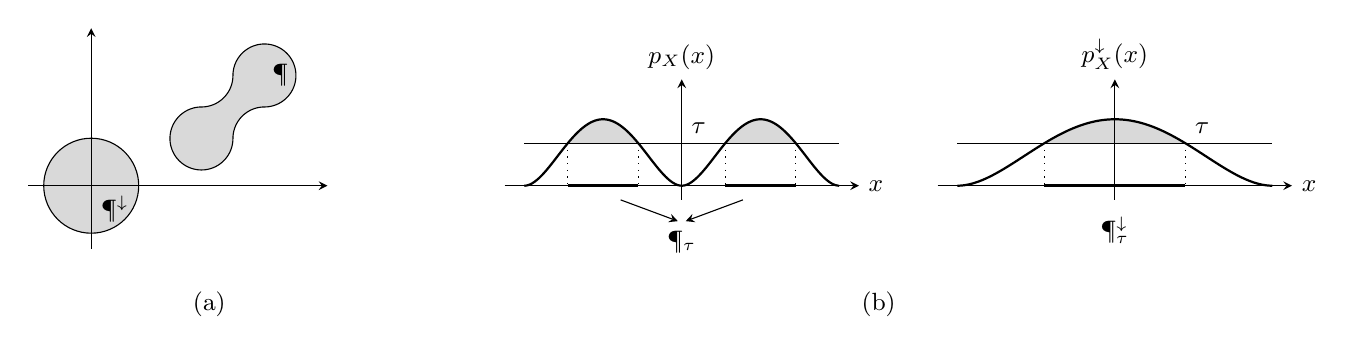
\begin{tikzpicture}
\shorthandoff{>}
%
\begin{scope}[scale=.4]
% Superficia 2*3 pi/4  + 2*2 - 2*pi/4 = 4+pi
\filldraw[draw=black,fill=gray!30]
   plot [domain=0:-270,samples=200] ({cos(\x)+3.5},{sin(\x)+1.5})
-- plot [domain=-90:0,samples=200] ({cos(\x)+3.5},{sin(\x)+3.5})
-- plot [domain=180:-90,samples=200] ({cos(\x)+5.5},{sin(\x)+3.5})
-- plot [domain=90:180,samples=200] ({cos(\x)+5.5},{sin(\x)+1.5})
-- cycle;
\draw (6,3.5) node {\small $\P$};
%
% superficia rearreglada
\filldraw[draw=black,fill=gray!30] (0,0) circle ({sqrt(1+4/pi)});
\draw (.75,-.75) node {\small $\P^\downarrow$};
%
% ejes
\draw[>=stealth,->] (-2,0)--(7.5,0);
\draw[>=stealth,->] (0,-2)--(0,5);
%
\end{scope}
%
%
%----------------------------------------
%
% p_X(x), P_tau...
\begin{scope}[xshift=7.5cm,yscale=1.8]
\pgfmathsetmacro{\t}{.3};
\pgfmathsetmacro{\xt}{sqrt(1-sqrt(32*\t/15))};
\pgfmathsetmacro{\dx}{5.5};% shift para p*(x)
\pgfmathdeclarefunction{studr}{1}{\pgfmathparse{(15/32)*((1-(#1)^2)^2)}}; %Student-r
%
% mezcla de Student-r 15/16 * (1-x^2)^2 (nu = 5) centrados en -1 y 1
% 15/32 (1-(x-a)^2)^2 > t iif (x-a)^2 < 1-sqrt(32*t/15)
% i.e. a-sqrt(1-sqrt(32*t/15)) < x < a+sqrt(1-sqrt(32*t/15))
\fill[domain=-1-\xt:-1+\xt,fill=gray!30] plot(\x,{studr(\x+1)}); % p(x) > tau, x < 0
\fill[domain=1-\xt:1+\xt,fill=gray!30] plot(\x,{studr(\x-1)}); % p(x) > tau, x > 0
\draw[thick,domain=-2:0,samples=100] plot(\x,{studr(\x+1)}); % p(x), x < 0
\draw[thick,domain=0:2,samples=100] plot(\x,{studr(\x-1)}); % p(x), x > 0
\draw (-2,\t)--(2,\t); \draw (0,\t) node[above right]{\small $\tau$}; % y = tau
%
% dominio P_tau
\draw[dotted] ({-1-\xt},{studr(\xt)})--({-1-\xt},0);
\draw[dotted] ({-1+\xt},{studr(\xt)})--({-1+\xt},0);
\draw[very thick] ({-1-\xt},0)--({-1+\xt},0);
\draw[>=stealth,->] ({-1+\xt/2},-.1)--(-.05,-.25);
%
\draw[dotted] ({1-\xt},{studr(\xt)})--({1-\xt},0);
\draw[dotted] ({1+\xt},{studr(\xt)})--({1+\xt},0);
\draw[very thick] ({1-\xt},0)--({1+\xt},0);
\draw[>=stealth,->] ({1-\xt/2},-.1)--(.05,-.25);
%
\draw (0,-.25) node[below]{\small $\P_\tau$};
%
% ejes
\draw[>=stealth,->] (-2.25,0)--(2.25,0) node[right]{\small $x$};
\draw[>=stealth,->] (0,-.1)--(0,.75) node[above]{\small $p_X(x)$};
%
%---------------------------
%
% 15/32 (1-(x-a)^2)^2 > t iif (x-a)^2 < 1-sqrt(32*t/15)
% i.e. a-sqrt(1-sqrt(32*t/15)) < x < a+sqrt(1-sqrt(32*t/15))
% Volumen 2*sqrt(1-sqrt(32*t/15))
% Por simetria, P_t* = [-2*sqrt(1-sqrt(32*t/15)) , 2*sqrt(1-sqrt(32*t/15))]
% da f*(x) = 15/32 (1-x^2/4)^2
\fill[domain=-2*\xt:2*\xt,fill=gray!30] plot({\x+\dx},{studr(.5*\x)}); % p*(x) > tau
\draw[thick,domain=-2:2,samples=200] plot({\x+\dx},{studr(.5*\x)});
\draw ({-2+\dx},\t)--({2+\dx},\t); \draw ({2*\xt+\dx},\t) node[above right]{\small $\tau$}; % y = tau
%
% dominio P_tau*
\draw[dotted] ({-2*\xt+\dx},{studr(\xt)})--({-2*\xt+\dx},0);
\draw[dotted] ({2*\xt+\dx},{studr(\xt)})--({2*\xt+\dx},0);
\draw[very thick] ({-2*\xt+\dx},0)--({2*\xt+\dx},0);
%
\draw (\dx,-.15) node[below]{\small $\P_\tau^\downarrow$};
%
% ejes
\draw[>=stealth,->] ({-2.25+\dx},0)--({2.25+\dx},0) node[right]{\small $x$};
\draw[>=stealth,->] (\dx,-.1)--(\dx,.75) node[above]{\small $p_X^\downarrow(x)$};
\end{scope}
%
\draw (1.5,-1.5) node{\small (a)};
\draw (10,-1.5) node{\small (b)};
\end{tikzpicture} \end{center}
%
\leyenda{(a):  Ilustraci\'on  del rearreglo  sim\'etrico  $\P^\downarrow$ de  un
  conjunto $\P$, siendo  $\P^\downarrow$ la bola centrada en  0 de mismo volumen
  que $\P$, en el caso bi-dimensional $d = 2$.  (b) Construcci\'on del rearreglo
  $p_X^\downarrow$:   dado  un   $\tau$,  se   busca  $\P_\tau$   y   se  deduce
  $\P_\tau^\downarrow$;  dado un  $x$, se  busca  el mayor  $t$ tal  que $x  \in
  \P_t^\downarrow$,    siendo    entonces   este    $t$    m\'aximo   igual    a
  $p_X^\downarrow(x)$;  adem\'as, por construcci\'on,  las superficies  en grise
  son iguales.}
  %
\label{Fig:MP:ensemblerearreglado}
\end{figure}
% =  \B  \left( 0  , r_\P  \right)$ con  $\frac{2
%    \pi^{d/2} r_\P^d}{\Gamma(d/2)} = |\P|$.

A partir de esta definici\'on del rearreglo, se puede ahora extender la noci\'on
de mayorizaci\'on del caso discreto al caso continuo de la manera siguiente:
%
\begin{definicion}[Mayorizaci\'on en el contexto continuo]
\label{Def:MP:MayorizacionContinua}
%
Una densidad de  probabilidad $p$ se dice mayorizada  por una distribuci\'on $q$
sii:
  %
  \[
  p \prec  q \qquad \mbox{sii}  \qquad \int_{\Bset(0,r)} p^\downarrow(x) \,  dx \le
  \int_{\Bset(0,r)} q^\downarrow(x) \, dx \quad \forall  \, r > 0, \quad \mbox{ y }
  \quad \int_{\Rset^d} p^\downarrow(x) \, dx = \int_{\Rset^d} q^\downarrow(x) \,
  dx,
  \]
  %
  %donde \ $\B(0,r) = \{ x \in \Rset^d:  \: \|x\| lge r \}$ \ es la bola centrada
  %en \ $0$ \ y de rayo  \ $r$ \ 
  (las \'ultimas integrales son obviamente iguales a 1).
\end{definicion}
%
\SZ{Equivalente de la curva de Lorentz???}


% =================== Transformacion de variables aleatorias =================== %

\seccion{Transformaci\'on de variables y vectores aleatorios}
\label{Sec:MP:Transformacion}

En esta secci\'on nos interesamos en  los efectos sobre una variable o un vector
aleatorio. Por ejemplo, en un juego con dos dados, nos puede interesar la ley de
la suma que dar\'ia el n\'umero de  casilla que debemos adelantar en un juego de
la oca.
%
\begin{teorema}[Transformaci\'on medible de un vector aleatorio]
\label{Teo:MP:TransformacionMedible}
%
  Sea  \  $X:  (\Omega,\A)  \mapsto  (\Rset^d ,  \B(\Rset^d))$  \  una  variable
  aleatoria,   y  \   $g:  (\Rset^d   ,  \B(\Rset^d))   \mapsto   (\Rset^{d'}  ,
  \B(\Rset^{d'}))$ \  una funci\'on  medible. Entonces,  \ $Y =  g(X)$ \  es una
  variable aleatoria  \ $(\Omega,\A)  \mapsto (\Rset^{d'} ,  \B(\Rset^{d'}))$. \
  Adem\'as, la medida imagen \ $P_Y$ \ est\'a vinculada \ a \ $P_X$ \ por
  %
  \[
  \forall \, B \in \B(\Rset^{d'}), \quad P_Y(B) = P_X(g^{-1}(B)).
  \]
\end{teorema}
%
\begin{proof}
  Este  resultado   es  obvio.  Siendo  $g$  una   funci\'on  medible  (recordar
  Def.~\ref{Def:MP:FuncionMedible}),  para  todo  $B  \in  \B(\Rset^{d'})$,  por
  definici\'on $g^{-1}(B) \in \B(\Rset^d)$.  Adem\'as, si $P_X$ es la medida (de
  probabilidad)  asociada  al  espacio  de   salida  de  $g$,  el  resultado  es
  consecuencia del teorema de la medida imagen~\ref{Teo:MP:MedidaImagen}.
  % , pagina~\pageref{Teo:MP:MedidaImagen}.
\end{proof}
%
\noindent (Ver ej.~\cite{Muk00, JacPro03, AthLah06, Bog07:v2, Coh13}).

Es  sencillo probar  que  cualquier combinaci\'on  de  funciones medibles  queda
medible, cualquier  producto (adecuado) de  funciones medibles queda  medible, y
que si  $\{ f_k \}_{k=1}^{d'}$  son $(\B(\Rset^d),\B(\Rset))$-medibles, entonces
$f        =        (f_1        ,        \ldots       ,        f_{d'})$        es
$(\B(\Rset^d),\B(\Rset^{d'}))$-medible~\cite{AthLah06}.

% \SZ{No se  todav\'ia si ser\'a \'util  tratar del caso de l\'imite  de series de
%   funciones medibles.}


Mencionamos   que si  $\X =  X(\Omega)$ es  discreto, entonces  $\Y =  g(\X) =
Y(\Omega)$ ser\'a discreto tambi\'en, y:
%
\begin{teorema}[Funci\'on de masa por transformaci\'on medible]
\label{Teo:MP:TransformacionMasa}
%
  Sean   $X$,   vector  aleatorio   $d$-dimensional   discreto,  $g:(\Rset^d   ,
  \B(\Rset^d)) \mapsto (\Rset^{d'} , \B(\Rset^{d'}))$ una funci\'on medible, e \
  $Y =  g(X)$ necesariamente discreto  $d'$-dimensional sobre $\Y =  g(\X)$.  La
  distribuci\'on de $Y$ est\'a vinculada con la de $X$ por la relaci\'on
  %
  \[
  \forall \, y \in \Y, \quad p_Y(y) = \sum_{x \in g^{-1}(y)} p_X(x).
  \]
\end{teorema}
%
\begin{proof}
  El resultado es inmediato.
\end{proof}
%
\noindent En particular,  si $g$ es inyectiva (necesariamente  biyectiva de $\X$
en $\Y$),  el vector  de probabilidad queda  invariante, $p_Y =  p_X$; solamente
cambian los estados.

Es  importante  mencionar que  con  $\Y$  discreto,  $\X$ no  es  necesariamente
discreto~\cite{AthLah06}. Por ejemplo, $Y = \uno_{X>0}$  es tal que $\Y = \{ 0 \;
1 \}$ a pesar de que $\X$ puede no ser discreto.

Tratar con  variables aleatorias continuas  resulta m\'as delicado. Vimos  en el
ejemplo   precedente   que   el   car\'acter   continuo   puede   perderse   por
transformaci\'on. De  la misma manera, en  un ejemplo de  la secci\'on anterior,
vimos  que  $Y =  X_1  \uno_{X_2>0}$ con  $X_i$  independientes  uniformes no  es
continua  ni  discreta.   En  el  enfoque  de  variables  continuas,  una  clase
importante de  funciones en las cuales  nos vamos a interesar  son las funciones
continuas (y diferenciables):
%
\begin{lema}[Continuidad y car\'acter medible]
\label{Lem:MP:ContinuidadCaracterMedible}
%
  Sea   $g:   \Rset^d   \mapsto   \Rset^{d'}$   continua.   Entonces,   $g$   es
  $(\B(\Rset^d),\B(\Rset^{d'}))$-medible.
\end{lema}
%
\begin{proof}
  Por continuidad,  la pre-imagen de  un abierto de  $\Rset^{d'}$ por $g$  es un
  abierto  de $\Rset^d$  y entonces  es en  $\B(\Rset^d)$. La  prueba  se cierra
  recordando  la definici\'on  de $\B(\Rset^{d'})$,  $\sigma$-\'algebra generada
  por los abiertos de $\Rset^{d'}$.
\end{proof}

En lo que sigue, nos interesamos m\'as especialmente en el caso de funciones $g:
(\Rset^d ,  \B(\Rset^d)) \mapsto (\Rset^d ,  \B(\Rset^d))$.  De hecho,  si $d' <
d$,   es    sencillo   llegar    al   caso   considerado    a\~nadiendo   $d-d'$
transformaciones. Por ejemplo, con $d = 2$ si nos interesa $X_1 + X_2$, se puede
considerar $\begin{bmatrix} X_1 + X_2 &  X_2 - X_1\end{bmatrix}^t$ y llegar a la
variable de inter\'es  por c\'alculo de marginal. Si $d' >  d$ la situaci\'on es
m\'as  delicada,   $g(Y)$  viviendo   sobre  una  variedad   $d$-dimensional  de
$\Rset^{d'}$.

En el  caso de vectores  aleatorios continuos $X$  que admitend una  densidad de
probabilidad,  una  pregunta  natural  es  entonces  saber  si  se  conserva  la
continuidad y la  existencia de una densidad, as\'i como  su forma. La respuesta
se da en el teorema siguiente~\cite{Bre88, JacPro03, AthLah06, Coh13, HogMck13}:
%
\begin{teorema}[Densidad de probabilidad por transformaci\'on continua inyectiva
  diferenciable]\label{Teo:MP:TransformacionInyectivaDensidad}
%
  Sea $X$, vector aleatorio $d$-dimensional  continuo que admite una densidad de
  probabilidad $p_X$, y sea \ $g:\Rset^d \mapsto \Rset^d$ una funci\'on continua
  inyectiva y diferenciable tal que
  %  ~\footnote{\modif{De  hecho,  se   puede  extender  el  resultado  para  un
  %      determinente del  Jacobiano cancelandose  en  un conjunto  de punto  de
  %     medida  de Lebesgue nula y en  los $y$ donde se  cancela el determinente
  %       del  Jacobiano,  la   densidad  va   a  ser   divergente  (divergencia
  %     integrable).}}
  $\left| \Jac_g \right| > 0$ (ver notaciones),
  %
  % donde   $\Jac_g$  denota   la  matriz   de  componentes   \  $\frac{\partial
  %   g_i}{\partial  x_j}$,  \ matriz  Jacobiana  de  la  transformaci\'on \  $g
  % \equiv \begin{bmatrix} g_1(x_1 , \ldots , x_d) & \cdots & g_d(x_1 , \ldots ,
  %   x_d) \end{bmatrix}^t$  \ y  \ $|\cdot|$ representa  el valor  absoluto del
  % determinante de la matriz.
  Sea  \  $Y =  g(X)$.   Entonces  $Y$ es  continua  y  admite  una densidad  de
  probabilidad $p_Y$ de soporte $\Y = g(\X) = Y(\Omega)$ tal que
  %
  \[
  \forall \,  y \in  \Y, \quad p_Y(y)  = p_X(g^{-1}(y))  \left| \Jac_{g^{-1}}(y)
  \right|.
  \]
\end{teorema}
%
\begin{proof}
  Por definici\'on, admitiendo $X$ una densidad y  siendo $g$ medible,
  %
  \[
  \forall \, B \in \B(\Rset^d),  \quad P_Y(B) = P_X(g^{-1}(B)) = \int_{g^{-1}(B)
    \cap \X} p_X(x) \, dx.
  \]
  %
  Por cambio de variables $x  = g^{-1}(y)$ (siendo $g$ inyectiva, el antecedente
  es \'unico por definici\'on) y  notando que $g\left( g^{-1}(B) \cap \X \right)
  = B \cap \Y$,
  %
  \[
  \forall \, B  \in \B(\Rset^d), \quad P_Y(B) =  \int_{B \cap \Y} p_X(g^{-1}(y))
  \, \left| \Jac_{g^{-1}}(y) \right| \, dy
  \]
  %
  lo que cierra la prueba~\footnote{La aparici\'on del Jacobiano viene del mismo
    enfoque que el cambio de variables en la integraci\'on de Riemann. De hecho,
    como lo  hemos visto, $\mu_L(B)  = |B|$ es  el volumen y de  la definici\'on
    misma del determinente, para cualquier matriz cuadrada el volumen se escribe
    \ $\mu_L(M  B) = |M B|  = |M| |B| =  |M| \mu_L(B)$ donde  la misma escritura
    $|\cdot|$ representa el valor absoluto  del determinente de una matriz. Esta
    notaci\'on se justifica precisamente por su significaci\'on de volumen, y el
    resultado   es  inmediato  para   $g(x)  =   M  x$.    La  forma   para  una
    transformaci\'on m\'as general se obtiene a partir de un desarollo de Taylor
    al orden  1 de  la transformaci\'on, haciendo  aparecer el  determinente del
    Jacobiano~\cite{AthLah06, Coh13}.}.
\end{proof}

El caso escalar puede ser visto como caso particular, dando:
%
\begin{corolario}
\label{Cor:MP:TransformacionInyectivaDensidadEscalar}
%
  Sean $X$, variable aleatoria continua  que admite una densidad de probabilidad
  $p_X$,   $g:\Rset  \mapsto   \Rset$  una   funci\'on  continua,   inyectiva  y
  diferenciable, e \ $Y = g(X)$.  Entonces $Y$ es continua y admite una densidad
  de probabilidad $p_Y$ tal que
  %
  \[
  \forall  \,   y  \in  \Y,   \quad  p_Y(y)  =  p_X(g^{-1}(y))   \left|  \frac{d
      g^{-1}(y)}{dy} \right|.
  \]
\end{corolario}
%
\noindent De hecho,  se pueden ver estos resultados  esquem\'aticamente como una
``conservaci\'on'' de  probabilidad, $p_X(x)  dx = p_Y(y)  dy$, el  volumen $dy$
estando  relacionado al  $dx$  a traves  de  la matriz  Jacobiana  (ver nota  de
pie~\ref{Foot:SZ:Jacobiana}).

Una  forma  alternativa  de derivar  este  corolario  consiste  en salir  de  la
funci\'on    de    repartici\'on,   notando    que    $g$   es    necesariamente
mon\'otona~\footnote{Notar que $P(X \ge x) = 1 - P(X < x) = 1 - P(X \le x) + P(X
  =  x)$, pero  siendo $X$  continua, $  P(X =  x) =  0$.}: si  $y  \notin \Y$,
necesariamente $p_Y = 0$ ($F_Y(y) = 1$ \ si \ $y > \sup \Y$ \ y \ $F_Y(y) = 0$ \
si \ $y < \inf \Y$) \ y para cualquier \ $y \in \Y$,
%
\[
F_Y(y) = P(Y \le y) = P(g(X) \le y) =
\left\{\begin{array}{lll}
P(X \le g^{-1}(y)) = F_X(g^{-1}(y)) & \mbox{si} & g \quad \mbox{es creciente}\\[2.5mm]
%
P(X \ge g^{-1}(y)) = 1 - F_X(g^{-1}(y)) & \mbox{si} & g \quad \mbox{es decreciente}
\end{array}\right..
\]
%
El  resultado  se  obtiene  calculando  las  derivadas  del  primer  y  \'ultimo
t\'erminos respecto de la variable transformada $y$.

Si $g$ no es inyectiva, $g^{-1}$  es multivaluada o multiforme. En este caso, se
puede todav\'ia  tratar el problema, particionando $\Rset^d$  en conjuntos donde
$g$ es inyectiva, dando
%
\begin{teorema}[Densidad   de   probabilidad   por   transformaci\'on   continua
  no inyectiva diferenciable]\label{Teo:MP:TransformacionNoInyectivaDensidad}
%
  Sea $X$, vector aleatorio $d$-dimensional  continuo que admite una densidad de
  probabilidad  $p_X$,  y sea  $g:(\Rset^d  ,  \B(\Rset^d))  \mapsto (\Rset^d  ,
  \B(\Rset^d))$  una  funci\'on continua  y  diferenciable.  Denotamos  $\left\{
    \X_{[k]} \right\}_{k=0}^m$ la partici\'on  de $\X$ tal que $\left| \Jac_g(y)
  \right| = 0$ sobre  $\X_{[0]}$, y para todo $k \ge 1$  se tiene \ $g: \X_{[k]}
  \mapsto  \Y$ \  inyectiva  y tal  que \  $\left|  \Jac_g(y) \right|  > 0$.   \
  Suponemos que $\X_{[0]}$ es de medida \modif{$P_X$} nula, notamos \ $g_k^{-1}$
  \ la funci\'on inversa de \ $g$ \ sobre \ $g(\X_{[k]})$ \ (rama $k$-\'esima de
  la  funci\'on   multivaluada  $g^{-1}$),  \  $\Jac_{g_k^{-1}}$   \  su  matriz
  Jacobiana, e \  $I(y) = \{ k \tq  y \in g(\X_{[k]}) \}$ \  los \'indices tales
  que  \  $y$  \  tiene  un   inverso  por  $g_k$.   Esto  es  ilustrado  en  la
  figura~\ref{Fig:MP:TransformacionVA} para $d = 1$.  Entonces $Y$ es continua y
  admite una densidad de probabilidad $p_Y$ tal que
  %
  \[
  \forall  \, y  \in \Y,  \quad p_Y(y)  = \sum_{k  \in  I(y)} p_X(g_k^{-1}(y))
  \left| \Jac_{g_k^{-1}}(y) \right|.
  \]
  %
  En el caso escalar $d = 1$ esto se formula
  %
  \[
  \forall \, y \in \Y, \quad  p_Y(y) = \sum_{k \in I(y)} p_X(g_k^{-1}(y)) \left|
    \frac{d g_k^{-1}(y)}{dy} \right|.
  \]
  %
  \noindent Esto se ilustra el la figura~\ref{Fig:MP:TransformacionVA}.
\end{teorema}
%
\begin{proof}
  \modif{Basta escribir \  $g^{-1}(B) = \bigcup_{k = 0}^m  \left( g^{-1}(B) \cap
      \X_{[k]} \right)$, uni\'on de borelianos disjuntos. Siendo $g^{-1}(B) \cap
    \X_{[k]} = g_k^{-1}(B)$, y siendo $\X_{[0]}$ de medida nula, se obtiene
  %
  \[
  P_Y(B) = P_X(g^{-1}(B)) = \sum_{k=1}^m \int_{g_k^{-1}(B)} p_X(x) \, dx
  \]
  %
  Se  nota ahora  que $g_k(g_k^{-1}(B)) = B \cap g(\X_{[k]})  \subset  B$ pero  no es  necesariamente
  $B$. Sin embargo, Por cambio de variables $x = g_k^{-1}(y)$ en cada integral, tenemos intonces
  %
  \[
  P_Y(B)  =   \sum_{k=1}^m \int_{B \cap g(\X_{[k]})}
  p_X\left( g_k^{-1}(y) \right) \left| \Jac_{g_k^{-1}}(y) \right| \, dy  =   \int_B
  \sum_{k=1}^m  \uno_{g(\X_{[k]})}(y) \, p_X\left( g_k^{-1}(y) \right) \left| \Jac_{g_k^{-1}}(y) \right| \, dy
  \]
  %
  Por definici\'on de $I(y)$, $y \in B \cap g(\X_{[k]}) \:\: \Leftrightarrow \:\: k \in I(y) $, lo conduce finalmente a
  %
  \[
  P_Y(B)  = \int_{B \cap  g(\X_{[k]})} \sum_{k  \in I(y)}  p_X\left( g_k^{-1}(y)
  \right) \left| \Jac_{g_k^{-1}}(y) \right| \, dy
  \]
 }
 % Basta escribir \ $B = \bigcup_{k  = 0}^m \left( B \cap g(\X_{[k]}) \right)$ \
 % uni\'on de  borelianos disjuntos, notar  que por consecuencia \  $g^{-1}(B) =
 % \bigcup_{k  =0}^m  g^{-1}\left( B  \cap  g(\X_{[k]})  \right)$  \ uni\'on  de
 % borelianos disjuntos  \ y  \ por linealidad  escribir la  integraci\'on sobre
 % $g^{-1}(B)$ como la suma de integrales sobre $g^{-1}\left( B \cap g(\X_{[k]})
 % \right)$. Se cierra la prueba  notando que \ $g^{-1}\left( B \cap g(\X_{[0]})
 % \right)$ es  necesariamente de  medida de Lebesgue  nula, siendo  la integral
 % nula y que \ $g^{-1}\left( B \cap g(\X_{[k]}) \right) = g_k^{-1}\left( B \cap
 %   g(\X_{[k]}) \right)$.
\end{proof}

\begin{figure}[h!]
\begin{center} 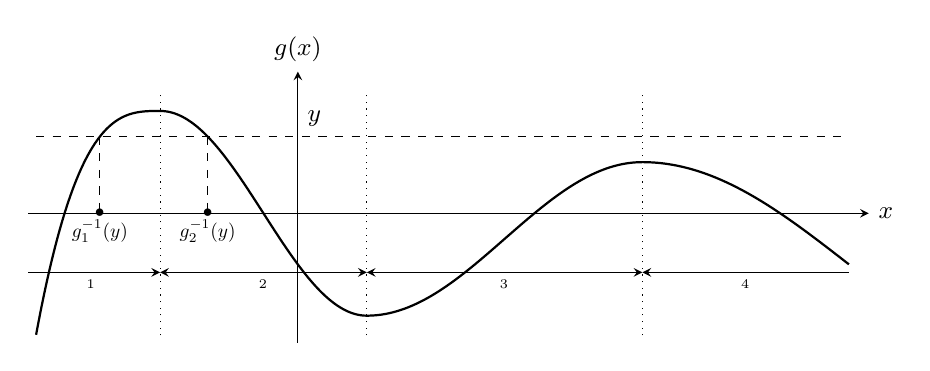
\begin{tikzpicture}%[scale=.9]
\shorthandoff{>}
%
\pgfmathsetmacro{\sx}{1.75};% x-scaling
%
% transformacion g' = 0 medida nula
\begin{scope}
%
\pgfmathsetmacro{\sy}{1.3};% y-scaling 
%
\draw[>=stealth,->] ({-1.9*\sx-.1},0)--({\sx*4+.25},0) node[right]{\small $x$};
\draw[>=stealth,->] (0,{\sy*(-3*.9^3+1)-.1})--(0,{\sy+.5}) node[above]{\small $g(x)$};
%
\draw[thick]
plot[domain=-1.9:-1,samples=100] ({\sx*\x},{\sy*(3*(\x+1)^3+1)})
-- plot[domain=-1:.5,samples=100] ({\sx*\x},{\sy*cos(120*(\x+1))})
-- plot[domain=.5:2.5,samples=100] ({\sx*\x},{\sy*(.75*sin(90*(\x-1.5))-.25)})
-- plot[domain=2.5:4,samples=100] ({\sx*\x},{\sy*(cos(60*(\x-2.5))-.5)})
;
%
\draw[dashed] ({-1.9*\sx},{.75*\sy})--({4*\sx},{.75*\sy});
\draw (0,{.75*\sy}) node[above right]{\small $y$};
%
\draw[dashed] ({-\sx*(1+(.25/3)^(1/3))},{.75*\sy})--({-\sx*(1+(.25/3)^(1/3))},0)
node[scale=.7]{$\bullet$} node[below,scale=.7]{$g_1^{-1}(y)$};
%
\draw[dashed] ({\sx*(acos(.75)/120-1)},{.75*\sy})--({\sx*(acos(.75)/120-1)},0)
node[scale=.7]{$\bullet$} node[below,scale=.7]{$g_2^{-1}(y)$};
%
%
\draw[dotted] ({-\sx},{-\sy-.25})--({-\sx},{\sy+.25});
\draw[>=stealth,->] ({-\sx*1.9-.1},-.75)--({-\sx},-.75);
\draw ({-1.5*\sx},-.75) node[below,scale=.8]{\small $\X_1$};
%
\draw[dotted] ({.5*\sx},{-\sy-.25})--({.5*\sx},{\sy+.25});
\draw[>=stealth,<->] ({-\sx},-.75)--({.5*\sx},-.75);
\draw ({-.25*\sx},-.75) node[below,scale=.8]{\small $\X_2$};
%
\draw[dotted] ({2.5*\sx},{-\sy-.25})--({2.5*\sx},{\sy+.25});
\draw[>=stealth,<->] ({.5*\sx},-.75)--({2.5*\sx},-.75);
\draw ({1.5*\sx},-.75) node[below,scale=.8]{\small $\X_3$};
%
\draw[>=stealth,<-] ({2.5*\sx},-.75)--({4*\sx},-.75);
\draw ({3.25*\sx},-.75) node[below,scale=.8]{\small $\X_4$};
\end{scope}
%
%
% % reparticion
% \begin{scope}[xshift=8.5cm]
% %
% \pgfmathsetmacro{\sy}{2};% y-scaling 
% %
% \draw[>=stealth,->] (-.6,0)--({\sx*4+.25},0) node[right]{\small $x$};
% \draw[>=stealth,->] (0,-.25)--(0,{\sy+.5}) node[above]{\small $F_X$};
% %
% \draw[thick] (-.5,0)--(0,0)--(\sx,{\sy/2})--({2*\sx},{\sy/2})
% -- plot[domain=2:3,samples=100] ({\sx*\x},{\sy*(1+(\x-2)^(3/2))/2})
% -- ({\sx*4},\sy);
% %
% \draw (\sx,0)--(\sx,-.1) node[below,scale=.9]{\small $1$};
% \draw ({2*\sx},0)--({2*\sx},-.1) node[below,scale=.9]{\small $2$};
% \draw ({3*\sx},0)--({3*\sx},-.1) node[below,scale=.9]{\small $3$};
% \draw (\sx,0)--(\sx,-.1) node[below,scale=.9]{\small $1$};
% %
% \draw (0,{\sy/2})--(-.1,{\sy/2}) node[left,scale=.7]{\small $1/2$};
% \draw (0,\sy)--(-.1,\sy) node[left,scale=.7]{\small $1$};
% %
% \draw ({\sx*2.25},-1) node{\small (b)};
% \end{scope}
%
\end{tikzpicture} \end{center}
%
\leyenda{Ilustraci\'on  de  una  transformaci\'on  $g$  no  inyectiva,  tal  que
  $\X_{[0]} = \{ x \tq g'(x) = 0 \}$, representado por los valores de $x$ en las
  lineas  punteadas. Es de  medida de  Lebesgue nula.   Se indican  los dominios
  $\X_{[k]}$.  La l\'inea discontinua da un nivel $y$ y los puntos en el eje $x$
  representan $g_k^{-1}(y), \: k \in I(y)$; en el ejemplo, $I(y) = \{ 1 \; 2 \}$
  \  y,   suponiendo  que  $\X  =   \Rset$,  \  $F_Y(y)   =  F_X(g_1^{-1}(y))  +
  1-F_X(g_2^{-1}(y))$.}
\label{Fig:MP:TransformacionVA}
\end{figure}

\begin{ejemplo}[Ejemplo de transformaci\'on no biyectiva]
\label{Ej:MP:TransformacionNoBiyectiva}
%
Sea $X$ definida sobre \ $\X =  \Rset$ \ y la transformaci\'on de variables \ $Y
= X^2$.  Se  tiene \ $y =  g(x) = x^2$, continua diferenciable  de derivada nula
sobre \ $\X_{[0]} = \{ 0 \}$,  de medida nula, cuyas inversas son \ $g_1^{-1}(y)
= - \sqrt{y}$ \ sobre \ $\X_{[1]}  = \Rset_{0,-}$ \ y \ $g_2^{-1}(y)
=   +  \sqrt{y}$   sobre  \   $\X_{[2]}  =   \Rset_{0,+}$;  luego   \   $p_Y(y)  =
\frac{p_X(\sqrt{y}) + p_X(-\sqrt{y})}{2 \sqrt{y}}$, \ sobre \ $\Y = \Rset_{0,+}$.
\end{ejemplo}

De nuevo, en el caso escalar, se puede salir de la funci\'on de repartici\'on
%
\[
F_Y(y) =  P(Y \le y) = P(  g(X) \le y )  = \sum_{k=1}^m P\left( X  \in \X_{[k]} \cap
  g_k^{-1}(-\infty \; y] \right)
\]
%
(siendo  $\X_{[0]}$  de medida  nula,  sobre  este  dominio la  probabilidad  es
cero). Sea $\Y_{[k]} = g_k(\X_{[k]})$. Ahora, si $y \notin I(y)$,
%
\[
P\left(   X   \in  \X_{[k]}   \cap   g_k^{-1}(-\infty  \;   y]  \right)   =
\left\{\begin{array}{lll}
%
P(X \in \X_{[k]}) & \mbox{si} & y > \sup \Y_{[k]}\\[2.5mm]
%
0 & \mbox{si} & y < \inf \Y_{[k]}
\end{array}\right.
\]
%
dando una derivada nula. Si $y \in I(y)$,
%
\[
P\left(   X   \in  \X_{[k]}   \cap   g_k^{-1}(-\infty  \;   y]  \right)   =
\left\{\begin{array}{lll}
%
F_X(g_k^{-1}(y)) - F_X(\inf \Y_{[k]}) & \mbox{si} & g_k \quad \mbox{es creciente}\\[2.5mm]
%
F_X(\sup \Y_{[k]}) - F_X(g_k^{-1}(y))  & \mbox{si} & g_k \quad \mbox{es decreciente}
\end{array}\right..
\]
%
El resultado sigue diferenciando estas expresiones. Se ilustra esto tambi\'en en
la figura~\ref{Fig:MP:TransformacionVA}.

Una tercera alternativa, a pesar de que sea delicado, es apoyarse en la teor\'ia
de distribuciones  y expresar como \  $\displaystyle p_Y(y) =  \int_\X p_X(x) \,
\delta(y-g(x)) \,  dx$, donde  se usa  la expansi\'on de  la funci\'on  delta en
t\'erminos de sus ceros:  \ $\delta(y-g(x)\,)= \sum_{k \in I(y)} \frac{1}{\left|
    g_k'\left(          g_k^{-1}          (y)          \right)          \right|}
\delta(x-g_k^{-1}(y))$~\cite{ManWol95}.

Es  importante   notar  que  la   condici\'on  $\X_{[0]}$  de  medida   nula  es
importante. Al  contrario, $Y$  no resulta  continua como se  puede ver  en el
ejemplo siguiente.
%
\begin{ejemplo}[Transformaci\'on con \modif{$P_X\left( \X_{[0]} \right) \ne 0$}]
\label{Ej:MP:X0MedidaNoNula}
%
Sea \ $X$ \ uniforme sobre  \ $\X = ( 3 \; 3)$ \ e \ $Y  = g(X)$ \ con \ $g(x) =
\Big(  1 +  \cos\left(  (|x|-1) \frac{\pi}{2} \right) \Big)  \uno_{(1 \;  3)}(|x|) +  2
  \uno_{[0    \;   1]}(|x|)$.     Esta    funci\'on   se    representa   en    la
  figura~\ref{Fig:MP:TransformacionVANoContinua}-(a).   Claramente, \  $g$  \ es
  continua y diferenciable sobre $\X$, pero con \ $\X_{[0]} = [ -1 \; 1]$ que no
  es  de  medida  nula.   Saliendo  de  $F_Y(y) =  P(g(X)  \le  y)$  se  calcula
  sencillamente  $F_Y(y) =  \frac23 \left(  1 -  \frac1\pi  \arccos(y-1) \right)
  \uno_{[0   \;   2)}   +   \uno_{[   2  \;   +\infty)}(y)$,   ilustrada   en   la
  figura~\ref{Fig:MP:TransformacionVANoContinua}-(b).   Claramente \ $F_Y$  \ es
  discontinua en \ $y = 2$: \ $Y$ \ no es continua.
  %
  \begin{figure}[h!]
  \begin{center} \begin{tikzpicture}%[scale=.9]
\shorthandoff{>}
%
\pgfmathsetmacro{\r}{.05};% radius arc non continuity F_X y/o p_X
%
% transformacion g' = 0 medida no nula
\begin{scope}
%
\draw[>=stealth,->] (-3.6,0)--(3.75,0) node[right]{\small $x$};
\draw[>=stealth,->] (0,-.25)--(0,2.5) node[above]{\small $g(x)$};
%
\draw[thick]
(-3.4,0)--(-3,0)--
plot[domain=-3:-1,samples=100] (\x,{1+cos(90*(1+\x))})--
(1,2)--
plot[domain=1:3,samples=100] (\x,{1+cos(90*(1-\x))})--
(3.5,0);
%
\draw (-3,0)--(-3,-.1) node[below,scale=.8]{\small $-3$};
\draw (-2,0)--(-2,-.1) node[below,scale=.8]{\small $-2$};
\draw (-1,0)--(-1,-.1) node[below,scale=.8]{\small $-1$};
\draw (1,0)--(1,-.1) node[below,scale=.8]{\small $1$};
\draw (2,0)--(2,-.1) node[below,scale=.8]{\small $2$};
\draw (3,0)--(3,-.1) node[below,scale=.8]{\small $3$};
%
\draw (0,1)--(-.1,1) node[left,scale=.8]{\small $1$};
\draw (-.1,2) node[above left,scale=.8]{\small $2$};
%
\draw[>=stealth,<->] (-3,-.5)--(-1,-.5); \draw (-2,-.5) node[below,scale=.9]{\small $\X_{[1]}$};
\draw[>=stealth,<->] (1,-.5)--(3,-.5); \draw (2,-.5) node[below,scale=.9]{\small $\X_{[2]}$};
\draw[>=stealth,<->] (-1,-.5)--(1,-.5); \draw (0,-.5) node[below,scale=.9]{\small $\X_{[0]}$};
%
\draw(0,-1.5) node{\small (a)};
\end{scope}
%
%
% reparticion
\begin{scope}[xshift=7cm]
%
\pgfmathsetmacro{\sx}{1.5};
\pgfmathsetmacro{\sy}{2};% y-scaling 
%
\draw[>=stealth,->] (-.6,0)--({3*\sx+.5},0) node[right]{\small $y$};
\draw[>=stealth,->] (0,-.25)--(0,{\sy+.25}) node[above]{\small $F_Y$};
%
\draw[thick] (-.5,0)--(0,0)--
plot[domain=0:2,samples=250] ({\sx*\x},{\sy*2*(1-acos(\x-1)/180)/3});
%
\draw ({2*\sx+\r},{2*\sy/3+\r}) arc (90:260:\r);
%--
\draw[dotted] ({2*\sx},{2*\sy/3})--({2*\sx},\sy);
\draw[thick] ({2*\sx},\sy) node[scale=.7]{$\bullet$}--({3*\sx},\sy);
%
\draw ({\sx},0)--({\sx},-.1) node[below,scale=.8]{\small $1$};
\draw ({2*\sx},0)--({2*\sx},-.1) node[below,scale=.8]{\small $2$};
\draw ({3*\sx},0)--({3*\sx},-.1) node[below,scale=.8]{\small $3$};
%
\draw (0,{2*\sy/3})--(-.1,{2*\sy/3}) node[left,scale=.7]{\small $2/3$};
\draw (0,\sy)--(-.1,\sy) node[left,scale=.7]{\small $1$};
%
\draw({1.75*\sx},-1.5) node{\small (b)};
\end{scope}
%
\end{tikzpicture} \end{center}
  %
  \leyenda{(a): Gr\'afica de $g(x) =  \Big( 1 + \cos\left( (|x|-1) \frac{\pi}{2}
    \right) \Big) \uno_{(1  \; 3)}(|x|) + 2 \uno_{[0  \; 1]}(|x|)$. Suponiendo que
    $\X  = (-3  \; 3)$,  claramente $\X_{[0]}  = [  -1 \;  1]$ no  es  de medida
    nula. (b): Para $X$ uniforme sobre  $\X$, la variable $Y = g(X)$ resulta con
    funci\'on de repartici\'on $F_Y$ no continua.  }
  \label{Fig:MP:TransformacionVANoContinua}
  \end{figure}
\end{ejemplo}

Un ejemplo de  cambio de transformaci\'on puede sevir a  calcular la densidad de
probabilidad de una suma:
%
\begin{ejemplo}[Distribuci\'on de la suma de vectores aleatorios]
\label{Ej:MP:Suma}
%
  Sean \ $X$ \ e \ $Y$ \ dos vectores aleatorios $d$-dimensionales conjuntamente
  continuos, de densidad de probabilidad conjunta $p_{X,Y}$, y sea el vector \[V
  = X +  Y.\] Queremos calcular la densidad de probabilidad  de $V$.  Para esto,
  se puede considerar la transformaci\'on biyectiva
  %
  \[
  g: (x,y) \mapsto (u,v) = (x,x+y).
  \]
  %
  Entonces
  %
  \[
  g^{-1}(u,v) = (u,v-u)
  \]
  %
  y la matriz Jacobiana es
  %
  \[
  J_{g^{-1}} = \begin{bmatrix} I & -I \\ 0 & I \end{bmatrix}
  \]
  %
  \modif{donde  la  identidad  \  $I$  \  y  la matriz  nula  \  $0$  \  son  en
    $\M_{d,d}(\Rset)$  conjuntos de  matrices  $d \times  d$ (ver  notaciones)}.
  Claramente\ $\left| J_{g^{-1}} \right| = 1$ \ as\'i que
  %
  \[
  p_{U,V}(u,v) = p_{X,Y}(u,v-u)
  \]
  %
  como lo podiamos intuir. Adem\'as, por marginalizaci\'on, inmediatamente
  %
  \[
  p_V(v) = \int_{\Rset^d} p_{X,Y}(u,v-u) \, du.
  \]
  %
  Si \ $X$ \ e \ $Y$  \ son independientes, \ $p_{U,V}(u,v) = p_X(u) p_Y(v-u)$ \
  y la f\'ormula integral se escribe
  %
  \[
  p_V(v) = \int_{\Rset^d} p_X(u) p_Y(v-u) \, du = \int_{\Rset^d} p_Y(u) p_X(v-u)
  \, du
  \]
  %
  (por  cambio  de variable  en  la  secunda  expresi\'on).  Esta  f\'ormula  es
  conocida    como     {\it    producto    de     convoluci\'on}    entre    las
  funciones~\footnote{\modif{Un  producto  de  convolution  entre  funciones  se
      define entre cualquieras funciones,  que sean densidades de probabilidad o
      no}.  Una  condici\'on suficiente para que existe  \modif{tal producto} es
    que  las funciones \modif{que  se convoluan}  sean $L^1$\modif{~\cite{Gol61,
        SteWei71, Pin09}  (es el caso  de densidad de probabilidad)}.}   $p_X$ y
  $p_Y$ \modif{y como lo podemos ver, es conmutativo}.
\end{ejemplo}


% ============================ Leyes condicionales ============================= %

\seccion{Leyes condicionales}
\label{Sec:MP:LeyesCondicionales}

Al  considerar un  par de  vectores aleatorios  \ $X$  \ e  \ $Y$,  una pregunta
natural  puede  ser c\'omo  caracterizar  el vector  $Y$  si  ``observamos $X  =
x$''.  En otras  palabras, la  pregunta es  describir la  ley de  $Y$ ``sabiendo
\modif{(o observando)}  que $X = x$''.  En lo que sigue,  para fijar notaci\'on,
consideramos $(X,Y): (  \Omega , \A) \mapsto (\Rset^{d_X}  \! \times \Rset^{d_Y}
\,   ,  \,   \B(\Rset^{d_X}  \!   \times  \Rset^{d_Y})   )$  tal   que   $X$  es
$d_X$-dimensional e $Y$ es $d_Y$-dimensional (incluyendo los casos escalares).


% ---------- Caso discreto

\paragraph{Caso $\boldsymbol{X}$ discreta:}
Un caso  sencillo a estudiar  es cuando $\X  = X(\Omega)$ es discreto.   En este
caso, para  cualquier $x  \in \X$, tenemos  $P_X(x) = P(X  = x)  \ne 0$ y  de la
definici\'on de  la probabilidad condicional Def.~\ref{Def:MP:ProbaCondicional},
$P(Y \in A | X = x) = \frac{P(Y \in A \cap X = x)}{P(X=x)}$ define una medida de
probabilidad que llamamos medida de probabilidad condicional y que denotaremos
%
\[
P_{Y|X=x}(A) = P(Y \in A | X = x).
\]
%
Siendo una medida de probabilidad, nos referimos a la subsecci\'on anterior para
definir una funci\'on de  repartici\'on tomando $\displaystyle A = \prod_{i=1}^d
(-\infty \; y_i]$, caracterizando completamente la medida de probabilidad:
%
\begin{definicion}[Funci\'on de repartici\'on condicional ($X$ discreto)]
\label{Def:MP:ReparticionCondicionalDiscreta}
%
  Por definici\'on, la funci\'on de repartici\'on condicional es,
  %
  \[
  \forall \:  x \in  \X, \: y  \in \Y, \quad  F_{Y|X=x}(y) =  P( \left. Y  \le y
  \right| X = x ) = \frac{P\left(  \left(Y \le y \right) \cap \left(X = x\right)
    \right)}{P\left(X = x\right)}.
  \]
\end{definicion}

Ahora, cuando $Y$  tambi\'en es discreta, se puede definir  la funci\'on de masa
discreta de probabilidad condicional, y si $Y$ es continua y admite una densidad
de probabilidad, se puede definir una densidad de probabilidad condicional:
%
\begin{definicion}[Funci\'on de masa o densidad de probabilidad condicional ($X$
  discreta)]
\label{Def:MP:ReparticionCondicionalDiscreta}
%
  Por  definici\'on,  cuando  $\Y$  es   discreta,  la  funci\'on  de  masa  de
  probabilidad condicional \modif{de $Y$ condicionalmente a $X = x$} es,
  %
  \[
  \forall \: x \in \X, \: y \in \Y, \quad p_{Y|X=x}(y) = P\left( \left. Y = y \right|
  X  =  x \right)  =  \frac{P\Big(  (Y  = y)  \cap  (X =  x) \Big)}{P(X = x)}.
  \]
  %
  Si $Y$ es continua, es sencillo ver que $P_{Y|X=x} \ll P_Y$, i.e., $P_Y(B) = 0
  \: \Rightarrow \: P_{Y|X=x}(B) = 0$.   Si $Y$ admite una densidad con respecto
  a la  medida de  Lebesgue, $P_Y \ll  \mu_L$ medida  de Lebesgue, es  claro que
  tambi\'en     $P_{Y|X=x}     \ll      \mu_L$,     y     por     teorema     de
  Radon-Nikod\'ym~\ref{Teo:MP:RadonNikodym}, $P_{Y|X=x}$  admite una densidad de
  probabilidad  (con   respecto  a  la  medida  de   Lebesgue)  que  denotaremos
  $p_{Y|X=x}$,
  %
  \[
  \forall \: B, \quad P_{Y|X=x}(B) = \int_B p_{Y|X=x}(y) \, dy.
  \]
  %
  A partir de la funci\'on de repartici\'on, obtenemos
  %
  \[
  p_{Y|X=x}(y) = \frac{\partial^{d_Y} F_{Y|X=x}(y)}{\partial y_1 \ldots \partial
    y_{d_Y}}.
  \]
\end{definicion}


% ---------- Caso continuo

\paragraph{Caso $\boldsymbol{X}$ continua admitiendo una densidad:}
Cuando  $X$  es   continua,  el  problema  es  m\'as   sutil  porque  $P(X=x)  =
0$. Entonces, no  se puede usar la definici\'on  de la probabilidad condicional,
siendo el  evento $(X=x)$ de probabilidad  nula.  Sin embargo,  se pueden seguir
los pasos  de R\'enyi~\cite[Cap.~5]{Ren} por ejemplo para  resolver el problema,
llegando a un resultado intuitivo como en el caso discreto.

Sea $B  \in \B(\Rset^{d_Y})$ y definimos  la medida $\nu_B(A) =  P\Big( \left( X
  \in A \right)  \cap \left( Y \in B \right) \Big)$  sobre $\left( \Rset^{d_Y} ,
  \B(\Rset^{d_Y}) \right)$.  Es sencillo ver que siendo dado $B$, $\nu_B$ define
una medida de  probabilidad. Adem\'as, $\nu_B \ll P_X$, i.e.,  $P_X(A) = P(X \in
A) = 0 \: \Rightarrow \: 0 = P\Big(  (X \in A) \cap (Y \in B) \Big) = \nu_B(A)$.
Por  teorema de  Radon-Nikod\'ym~\ref{Teo:MP:RadonNikodym},  $\nu_B$ admite  una
densidad $g_B$ con respecto a $P_X$,
%
\[
\forall \: A, \quad P\Big( (X \in A)  \cap (Y \in B) \Big) = \int_A g_B(x) \,
dP_X(x).
\]
%
Claramente \ $g_B \ge 0$, \ y de \ $P(X \in A) = P\Big( (X \in A) \cap (Y \in B)
\Big) + P\Big( (X \in A) \cap  (Y \in B) \Big)$, \ie $\displaystyle 0 \le P\Big(
(X \in A) \cap (Y \in B) \Big)  = \int_A dP_X(x) - \int_A g_B(x) \, dP_X(x)$, se
obtiene \ $0  \le g_B \le 1$.  En  realidad, tenemos \ $g_B \le  1$ \ $P_X$-casi
siempre, pero olvidando esta subtilesa, llamaremos la funci\'on \ $g_B$ \ medida
de probabilidad condicional y, por continuaci\'on, la funci\'on de repartici\'on
condicional:
%
\begin{definicion}[Medida   de  probabilidad   y   funci\'on  de   repartici\'on
  condicional ($X$ continuo)]
\label{Def:MP:MedidaCondicional}
%
  La medida de probabilidad condicional de $P_{Y|X=x}$ es definida tal que
  %
  \[
  \forall \: (A,B) \in \X \times \Y,  \quad P\Big( (X \in A) \cap (Y \in B) \Big)
  = \int_A P_{Y|X=x}(B) \, dP_X(x).
  \]
  %
  Tomando $B  = \optimes_i  (-\infty \; y_i]$  se obtiene la  funci\'on de
  repartici\'on condicional a partir de
  %
  \[
  \forall \: (A,B) \in \X \times \Y, \quad P\Big( (X \in A) \cap (Y \le y) \Big) =
  \int_A F_{Y|X=x}(y) \, dP_X(x).
  \]
  %
  Ad\'emas, si $X$ admite una densidad  de probabilidad $p_X$, $dP_X = p_X dx$ y
  tomando $A = \optimes_i (-\infty \; x_i]$ se obtiene
  %
  \[
  F_{X,Y}(x,y) = \int_{\optimes_i (-\infty \; x_i]} F_{Y|X=x}(y) \, p_X(x)
  \, dx
  \]
  %
  o, por diferenciaci\'on, para cualquier $y \in \Y$,
  %
  \[
  F_{Y|X=x}(y)   =  \frac{\frac{\partial^{d_X}}{\partial  x_1   \ldots  \partial
      x_{d_X}} F_{X,Y}(x,y)}{p_X(x)}.
  \]
\end{definicion}
%
\noindent Nota: Tomando  $A = \X$, de la primera f\'ormula  que define la medida
de probabilidad condicional se recupera  el equivalente continuo de la f\'ormula
de probabilidad total, que se escribe con la densidad $dP_X = p_X d\mu_L$ si $X$
admite una densidad.

Por \'ultimo, si $(X,Y)$ admite una  densidad, en sencillo ver  que $P_{Y|X=x} \ll
\mu_L$,  y entonces  \ $P_{Y|X=x}$  \ admite  una densidad  que  llamaremos {\it
  densidad de probabilidad condicional}. Sean $A \in \B(\X)$ y $B$,
%
\begin{eqnarray*}
P\Big( (X \in A) \cap (Y \in B) \Big) & = & \int_{A \times B} p_{X,Y}(x,y) \, dx \, dy\\[2mm]
%
& = & \int_B \left( \int_A \frac{p_{X,Y}(x,y)}{p_X(x)} \, dy \right) p_X(x) \, dx
\end{eqnarray*}
%
Entonces, si $p_X(x) \ne 0$, tenemos
%
\[
P_{Y|X=x}(A) = \int_A \frac{p_{X,Y}(x,y)}{p_X(x)} \, dy.
\]
%
\begin{teorema}[Densidad de probabilidad condicional]
\label{Def:MP:DensidadCondicional}
%
  Si  $(X,Y)$ admite  una densidad  de probabilidad,  la medida  de probabilidad
  condicional  $P_{Y|X=x}$  admite  una   densidad,  llamada  {\it  densidad  de
    probabilidad condicional} definida por
  %
  \[
  \forall \: x \in \X, \quad p_{Y|X=x}(y) = \frac{p_{X,Y}(x,y)}{p_X(x)}
  \]
  %
  definida  sobre $\Y$. Claramente,  a partir de  la funci\'on  de repartici\'on
  condicional resulta que
  %
  \[
  p_{Y|X=x} = \frac{\partial^{d_Y}  F_{Y|X=x}}{\partial y_1 \ldots \partial y_{d_Y}}.
  \]
\end{teorema}

De hecho, esta  construcci\'on rigurosa coincide con la  intuici\'on que podemos
tener en este  caso continuo. Por ejemplo, podemos  pensar a $F_{Y|X=x}(y)$ como
caso l\'imite de $P(\left. Y \le y \right|  x \le X \le x+\delta x) = \frac{P( Y
  \le  y \:  \cap \:  x \le  X \le  x+\delta x)}{P(x  \le X  \le x+\delta  x)} =
\frac{F_{X,Y}(x+\delta  x ,  y) -  F_{X,Y}(x  , y)}{F_X(x+\delta  x) -  F_X(x)}$
cuando \ $\delta  x$ \ tiende a 0.   En el caso escalar, se  calcula por ejemplo
haciendo un  desarrollo de Taylor del numerador  y del denominador a  orden 1, o
usando la regla de l'H\^opital~\footnote{De hecho, esta regla es debido al suizo
  J.  Bernoulli  que tuvo  un acuerdo financiero  con el  Guillaume Fran\c{c}ois
  Antoine, marqu\'es  de l'H\^opital, permitiendolo de  publicar unos resultados
  de Bernoulli bajo  su nombre.}  para re-obtener la  funci\'on de repartici\'on
condicional   de   la   definici\'on~\ref{Def:MP:FRCondicional}.  En   el   caso
multivariado,  hace  falta  hacer  los  desarollos hasta  el  orden  $d_X$  para
concluir.

Notar  que:
%
\begin{itemize}
\item si $X$ e $Y$ son independientes,
  %
  \[
  p_{Y|X=x} = p_Y;
  \]
%
\item por  la expresi\'on \ $p_{Y|X=x}(y) =  \frac{p_{X,Y}(x,y)}{p_X(x)}$, \ por
  integraci\'on con respecto a $y$ obtenemos la condici\'on de normalizaci\'on
  %
  \[
  \int_{\Rset^{d_Y}} p_{Y|X=x}(y) \, dy = 1;
  \]
%
\item escribiendo  \ $p_{X,Y}(x,y)  = p_{Y|X=x}(y) \,  p_X(x) =  p_{X|Y=y}(x) \,
  p_Y(y)$, \ se obtiene
  %
  \[
  p_{Y|X=x}(y)   =  \frac{p_{X|Y=y}(x) \,   p_Y(y)}{p_X(x)}   =  \frac{p_{X|Y=y}(x)
    \, p_Y(y)}{\displaystyle \int_{\Rset^{d_Y}} p_{X|Y=y}(x) \, p_Y(y) \, dy},
  \]
  %
  equivalente continuo, con densidades, de la f\'ormula de Bayes;
%
\item  por la  expresi\'on  \ $p_{X,Y}(x,y)  =  p_{Y|X=x}(y) \,  p_X(x)$, \  por
  integraci\'on con respecto a $x$ obtenemos
  %
  \[
  p_Y(y) = \int_{\Rset^{d_X}} p_{Y|X=x}(y) \, p_X(x) \, dx,
  \]
  %
  generalizaci\'on de la f\'ormula de  probabilidades totales al caso continuo con
  densidad de probabilidad.
\end{itemize}

Volvemos al ejemplo~\ref{Ej:MP:Suma}:
%, pagina~\pageref{Ej:MP:Suma}:
%
\begin{ejemplo}[Distribuci\'on condicional de la suma de vectores aleatorios]
\label{Ej:MP:SumaCond}
%
  Sea   \   $V  =   X   +   Y$,  \   con   \   $X$  \   e   \   $Y$  \   vectores
  $d$-dimensionales.  Introduciendo \  $U =  X$  \ obtuvimos  \ $p_{U,V}(u,v)  =
  p_{X,Y}(u,v-u)$  \ dando  tambi\'en \  $\displaystyle p_V(v)  = \int_{\Rset^d}
  p_{X,Y}(u,v-u) \, du$. Entonces, recordando que $U = X$, se obtiene
  %
  \[
  p_{V|X=x}(v)            =            \frac{p_{X,Y}(x,v-x)}{p_X(x)}           =
  \frac{p_{X,Y}(x,v-x)}{\displaystyle \int_{\Rset^d} p_{X,Y}(x,v-x) \, dv},
  \]
  %
  dando en el caso \ $X$ \ e \ $Y$ \ independientes
  %
  \[
  p_{V|X=x}(v) = p_Y(v-x).
  \]
  %
  Esto corresponde a la  intuci\'on de que, con $V = X + Y$,  fijando $X = x$ el
  vector aleatorio  $V$ es nada  m\'as que $Y$  desplazado en $x$. Pero  hay que
  tomar muchas precauciones con  este razonamiento, valido \'unicamente cuando \
  $X$  \ e  \  $Y$ \  son independientes.   En  caso contrario,  fijando $X$  no
  coincide con un desplazamiento por la dependencia (esquemat\'icamente, fijando
  $X$ no s\'olo mueve \ $Y$ \ sino que ``cambia'' su estad\'istica).
\end{ejemplo}


% =================================== Momentos ================================= %

\seccion{Esperanza, momentos, identidades y desigualdades}%funciones generadoras}
\label{Sec:MP:esperanzamomento}


%%%%%%%%%%%%%%%%%%%%%%%%%%%%%%%%%%%%%%%%%%%%%%%%%%%%%%%%%%%%%%%%%%%%%%%%%%

\modif{Como lo hemos introducido, la  noci\'on formal de probabilidad naci\'o en
  el  contexto  de  juego (cartas,  dados),  bajo  entre  otros el  impulso  del
  matem\'atico  italiano y  jugador de  dados y  cartas Gerolamo  Cardano  en el
  siglo~{XVI},  y a\'un  m\'as bajo  el trabajo  muy profundo  de  la dinast\'ia
  Bernoulli,   y  en   particular  Jacob   Bernoulli~\cite[en  lat\'in]{Ber1713}
  o~\cite{Ber13:2}.   En particular,  Bernoulli  se interes\'o  no solamente  al
  resultado de un  sorteo, impredictible, pero en lo que pasa  cuando se hace un
  gran num\'ero de sorteos.  As\'i sali\'o la idea de ``resultado promedio''. De
  hecho,  la noci\'on  de  promedio es  probablemente  debido a  B.  Pascal:  se
  encuentran, por lo menos semillas de  esta noci\'on en una carta que mand\'o a
  Fermat  en   1654~\cite{DavEdw01},  o  un   poco  m\'as  tarde  debido   a  C.
  Huygens~\cite{Huy57, DavEdw01, Hal90}~\cite{De hecho, aparece con una visi\'on
    frecuencista  y en  el contexto  discreto  finito. Sin  embargo, aparece  el
    termino  ``expectatio'' en  lat\'in,  dando esperanza  o ``expectation''  en
    ingl\'es, tratando de un valor  promedio.}. Bernoulli hizo el paso decisivo,
  y en  su trabajo, ha  ido m\'as  all\'a: prob\'o la  ley de gran  n\'umero que
  vamos a ver m\'as  adelante. Sin ir tan lejos, en el  caso de una variable $X$
  aleatoria discreta (ej. un dado, que puede tomar valores en $\{ 1 \; \ldots \;
  6 \}$), haciendo varios sorteos, el promedio de estes sorteos va a ser $\sum_i
  \widetilde{p}_i  x_i$ con  $x_i$ los  valores que  puede tomar  la  variable y
  $\widetilde{p}_i$ la  proporci\'on de  $x_i$ que se  obtuvo en el  sorteo.  De
  hecho, intuitivamente  (es la  visi\'on frecuencista), $\widetilde{p}_i$  va a
  tender a $p_i = P(X=x_i)$ cuando el n\'umero de sorteo tiende al infinito.  La
  definici\'on del valor promedio, o media, de una variable aleatoria cualquiera
  se formaliza  mas rigorosamente en  en marco de  la teoria de la  medida, pero
  coincide con la intuici\'on.}


% ================================= Media

\subseccion{Media de un vector aleatorio}
\label{Ssec:MP:VectorMedio}


Una  variable aleatoria  $X$  tiene asociado  un  {\it promedio}  o {\it  media}
(tambi\'en  llamado   {\it  valor  esperado  o  de   expectaci\'on  o  esperanza
  matem\'atica})  que se  obtiene pesando  cada valor  de $X$  con la  medida de
probabilidad asociada a ese valor~\cite{AshDol99, AthLah06},
%
\begin{definicion}[Media o valor/vector medio]
\label{Def:MP:ValorMedio}
%
  Formalmente, la media de  una variable aleatoria $X$ \underline{integrable} es
  definida por
  %
  \[
  \Esp[X] = \int_\Omega X(\omega) \, dP(\omega).
  \]
  %
  Por    el    teorema    de    la    medida    imagen~\ref{Teo:MP:MedidaImagen},
  %pagina~\pageref{Teo:MP:MedidaImagen}, 
  esta media  se escribe tambi\'en a  partir de la medida  de probabilidad $P_X$
  como
  %
  \[
  \Esp[X] = \int_\Rset x \, dP_X(x).
  \]
  %
  En  el caso vectorial  $d$-dimensional, hay  que entender  la media,  o vector
  medio, como  un vector de componentes  $i$-\'esima la media  $\Esp[X_i]$ de la
  componente $i$-\'esima $X_i$ de $X$, dando
  %
  \[
  \Esp[X] = \int_{\Rset^d} x \, dP_X(x).
  \]
  %
  A veces,  se encuentra  tambi\'en la notaci\'on  \ $\langle  x \rangle$ \  o \
  $\langle  x  \rangle_{p_X}$  \  para  el  valor  medio,  especialmente  en  la
  literatura de f\'isica.
\end{definicion}
%
La secunda formulaci\'on  del valor medio se proba  sencillamente, empezando por
$X =  \un_A$ para unos $A \in  \B(\Rset)$.  Entonces $P_X =  (1-P(A)) \delta_0 +
P(A)  \delta_1$.  Luego  $\displaystyle \int_\Omega  \un_A(\omega)  dP(\omega) =
P(A) = (1-P(A)) \times 0 + P(A)  \times 1 = \int_\Rset x dP_X(x)$.  Se cierra la
prueba  con  el  teorema~\ref{Teo:MP:MedibleLimite}  dando  cualquier  funci\'on
medible    como    l\'imite    de    funciones    escalonadas,    y    por    la
definici\'on~\ref{Def:MP:IntegracionReal} de la  integral de cualquier funci\'on
medible.

Luego,   de    la   distribuci\'on   marginal    $\displaystyle   P_{X_i}(B)   =
\int_{\Rset^{i-1}   \times   B   \times   \Rset^{d-i}}  dP_X(x)$,   se   obtiene
$\displaystyle  \Esp[X_i] = \int_{\Rset^d}  x_i \,  dP_X(x)$, dando  la \'ultima
formulaci\'on en el caso vectorial.

Una variable  aleatoria $X$ se dice  integrable cuando $E[|X|] <  \infty$. De la
misma  manera, un  vector aleatorio  admite  una media  si y  solamente si  cada
componente  es   integrable.  Veremos  m\'as  adelante   que  existen  variables
aleatorias que no admiten una media.

M\'as  all\'a  de  la formulaci\'on  matem\'atica,
%  de  la  media \  
$\Esp[X]$ \  representa la posici\'on alrededor  de la cual  se ``distribuye las
probabilidades de occurencia''. Es  el equivalente probabil\'istico de centro de
gravedad o barycentro en mec\'anica.

En el  caso de variables  aleatorias discretas, de soporte  \modif{$\X$ discreto
  finito o numerable,} inmediatamente
%
\[
\Esp[X] = \modif{\sum_{x \in \X} x \, P(X = x) = \sum_{x \in \X} x \, p_X(x).}
\]
%
\noindent  Fijense de  que $\Esp[X]$  no partenece  necesariamente a  $\X$:
%
\begin{ejemplo}
\label{Ej:MP:Uniforme3Estados}
%
  Sea \  $X$ \  uniforme sobre \  $\X = \{  1 \; 3  \; 7 \}$,  \ie \
  $\forall \,  i \in \X, \quad  P(X = i) =  \frac13$. \ Se calcula  $\Esp[X] = 1
  \times \frac13  + 3 \times \frac13  + 7 \times \frac13  = \frac{11}{3} \not\in
  \X$.  Tampoco es el promedio de los valores extremos.
\end{ejemplo}
%
\noindent Cuando \ $|\X| = +\infty$, \ $X$ \ no es necesariamente integrable:
%
\begin{ejemplo}
\label{Ej:MP:DiscretaSinMedia}
%
Sea  \ $\X  = \Nset^*$  \ con  \modif{$P(X =  x) =  \frac{6}{\pi^2 \,  x^2}$}. \
Claramente, \modif{$\sum_x\frac{6}{\pi^2 \, x}$} diverge, as\'i que $X$ no tiene
una media.
\end{ejemplo}

En el caso de vectores  aleatorios continuos, obtenemos la expresi\'on siguiente
de la media (o vector medio):
%
\[
\Esp[X] = \int_{\Rset^d} x \, p_X(x) \, dx.
\]
%
\noindent Las mismas observaciones que  hicimos en el caso discreto se encuentra
en el caso continuo:
%
\begin{ejemplo}
\label{Ej:MP:MediaNoEnX}
%
Sea \ $X$ \ de densidad de  probabilidad \ $p_X(x) = \frac12 \un_{[0 \; 1)}(x) +
\frac{3   \sqrt{x-2}}{4}   \un_{[2   \;   3)}(x)$  \   como   ilustrado   figura
Fig.~\ref{Fig:MP:ProbaContinua}.
%,    pagina~\pageref{Fig:MP:ProbaContinua}.    
Se calcula \ $\Esp[X] = \frac{31}{20} \not\in \X = [0 \; 1] \cup [2 \; 3]$.
\end{ejemplo}
%
\begin{ejemplo}
\label{Ej:MP:VariableCauchySinMedia}
%
  Un ejemplo  de vector aleatorio no  teniendo media es  dado en el caso  de una
  distribuci\'on de Cauchy-Lorentz (ver  m\'as adelante) \ $\displaystyle p_X(x)
  = \frac{\alpha}{\left( 1 + x^t x \right)^{\frac{d+1}{2}}}$ \ donde $\alpha$ es
  un factor de normalizaci\'on.
\end{ejemplo}

En el caso general, para calcular  la media, hay que pasar por la distribuci\'on
$P_X$, como en el ejemplo~\ref{Ej:MP:Mixta}:
%  pagina~\pageref{Ej:MP:Mixta}:
%
\begin{ejemplo}[Continuaci\'on del ejemplo~\ref{Ej:MP:Mixta}]
\label{Ej:MP:EspMixta}
%
Sea $X =  V \, \un_{U <  \frac12} + \un_{U \ge \frac12}$  \ con \ $U$ \  y \ $V$
variables aleatorias  independientes de distribuci\'on uniformas sobre  \ $[0 \;
1)$, \ie  $p_U(x) = \un_{[0 \;  1)}(x)$. \ De \  $(X \in B)  \: \Leftrightarrow \:
\left( \left( U < \frac12 \right) \cap \left( V \in B \right) \right) \, \cup \,
\left( \left( U \ge \frac12 \right) \cap  \left( 1 \in B \right) \right)$, \ del
hecho de que  los eventos de la uni\'on son incompatibles  y de la independencia
de $U$ y $V$ (o saliendo de la funci\'on de repartici\'on), se obtiene $P_X(B) =
\frac12  P_V(B)  + \frac12  \delta_1(B)$.   A  continuaci\'on, \  $\displaystyle
\Esp[X] = \frac12 \int_\Rset dP_V(x) + \frac12 \int_\Rset d\delta_1(x) = \frac12
\int_\Rset p_V(x)  \, dx + \frac12  \times 1 =  \frac12 \int_0^1 dx +  \frac12 =
\frac34$.
\end{ejemplo}

\

Una nota intersante  es de que, en el  caso escalar, \modif{para} \ $X  \ge 0$ \
admitiendo una media, se obtiene
%
\[
\Esp[X]  = \int_{\Rset_+} P(X  > t)  \, dt  = \int_{\Rset_+}  \left( 1  - F_X(t)
\right) \, dt.
\]
%
Se proba saliendo  de \ $\displaystyle x = \int_0^x  dt = \int_{\Rset_+} \un_{(t
  \; +\infty)}(x)  \, dt$ \ dando  \ $\displaystyle \Esp[X]  = \int_\Rset \left(
  \int_{\Rset_+}   \un_{(t  \;  +\infty)}(x)   \,  dt   \right)  \,   dP_X(x)  =
\int_{\Rset_+} \left(  \int_\Rset \un_{(t \; +\infty)}(x) \,  dP_X(x) \right) \,
dt$ \ por el teorema de Fubini Th.~\ref{Teo:MP:Fubini}.
%pagina~\pageref{Teo:MP:Fubini}. 
Se cierra la prueba observando que la integral interior es nada m\'as que $P(X >
t)$.   En   el  caso  discreto  con   $\X  =  \Nset$,   viene  inmediatamente  \
\modif{$\displaystyle  \sum_{t  \in  \Nset}   P(X  >  t)$}  que  podemos  probar
directamente saliendo de \modif{$P(X = t) = P(X  > t) - P(X > t-1)$}. En el caso
de variable  admitiendo una densidad,  se \modif{lo} obtiene  tambi\'en haciendo
una  integraci\'on  por partes~\footnote{En  el  caso  discreto,  hay que  tener
  precauciones separando la series de una diferencia de terminos. En el caso $X$
  continuo admitiendo una densidad, hay  que estudiar bien el coomportamiento de
  $t \mapsto (1-F_X(t))$ al infinito.}

Esta f\'ormula se aplica al ejemplo~\ref{Ej:MP:Mixta} que tratamos:
%
\begin{ejemplo}[Continuaci\'on del ejemplo~\ref{Ej:MP:Mixta}]
\label{Ej:MP:EspMixtaPositiva}
%
Sea $X =  V \, \un_{U <  \frac12} + \un_{U \ge \frac12}$  \ con \ $U$ \  y \ $V$
variables aleatorias  independientes de distribuci\'on uniformas sobre  \ $[0 \;
1)$.  \modif{Tratando de este ejemplo, o}btuvimos
% pagina~\pageref{Ej:MP:Mixta} 
\  $F_X(x)  = \frac{x}{2}  \un_{[0  \; 1)}(x)  +  \un_{[1  \; +\infty)}(x)$.   A
continuaci\'on,  reobtenemos \  $\displaystyle  \Esp[X] =  \int_0^1  \left( 1  -
  \frac{x}{2} \right) \, dx = \frac34$.
\end{ejemplo}.

\

Terminamos  esta  secci\'on con  la  propiedad  de  linealidad de  la  esperanza
matem\'atica $\Esp$,  como consecuencia de  la linealidad de la  integraci\'on y
definici\'on de la distribuci\'on  marginal: para cualquier conjunto de vectores
aleatorios \  $\{ X_i \}$  \ integrables, cualquieras  matrices \ $\{ C_i  \}$ \
dadas  (deterministicas)  de  dimensiones  compatibles   con  las  de  \  $X$  \
(incluyendo el caso escalar), y $b$ vecto dado (cierto),
%
\[
\Esp\left[ \sum_i C_i X_i + b \right] = \sum_i C_i \Esp\left[ X_i \right] + b
\]
%
(la integrabilidad de la suma se proba a partir de la desigualdad triangular).



% ================================= Momentos

\subseccion{Momentos de un vector aleatorio}
\label{Ssec:MP:Momentos}

Si $X$ es una variable aleatoria, para cualquier funci\'on medible $f$, \ $f(X)$
tambi\'en lo es.   Se puede entonces definir su valor medio,  si existe. A pesar
de necesitar evaluar  la distribuci\'on de probabilidad de $Y  = f(X)$, el valor
medio se calcula a partir del de $X$:
%
\begin{teorema}[Teorema de transferencia]
\label{Teo:MP:Transferencia}
%
  Sea  \ $X$  \ un  vector  aleatorio $d$-dimensional  y \  $f: \Rset^d  \mapsto
  \Rset^{d'}$ \ una funci\'on medible tal que $f(X)$ sea integrable. Entonces
  %
  \[
  \Esp\left[   f(X)  \right]   =  \int_\Omega   f(X(\omega))  \,   dP(\omega)  =
  \int_{\Rset^{d'}} f(x) \, dP_X(x).
  \]
  %
  En particular, en el caso $\X = X(\Omega)$ discreto se obtiene
  %
  \[
  \Esp\left[ f(X) \right] = \modif{\sum_{x \in \X} f(x) \, P(X = x)}
  \]
  %
  y para $X$ continuo admitiendo una densidad de probabilidad
  %
  \[
  \Esp\left[ f(X) \right] = \int_{\Rset^d} f(x) \, p_X(x) \, dx.
  \]
\end{teorema}
%
\begin{proof}
  Sea $B \in \B(\Rset^d)$ \ y consideramos \ $f(x) = \un_B(x)$. Entonces, $\Y
  = \{  0 \;  1 \}$ y inmediatamente
  %
  \[
  P_Y = P_X(B) \, \delta_1 + (1-P_X(B)) \, \delta_0.
  \]
  %
  Entonces
  %
  \[
  \Esp[f(X)]  =  \int_\Rset  P_X(B)  \,  d\delta_1 +  \int_\Rset  (1-P_X(B))  \,
  d\delta_0 = P_X(B) = \int_{\Rset^d} \un_B(x) \, dP_X(x).
  \]
  %
  En el caso  $d' = 1$, para $f  \ge 0$, se cierra entonces la  prueba usando el
  teorema~\ref{Teo:MP:MedibleLimite},
  % pagina~\pageref{Teo:MP:MedibleLimite},
  escribiendo \  $f$ \  como l\'imite creciente  de una sucesi\'on  de funciones
  escalonadas,    y   la    definici\'on~\ref{Def:MP:IntegracionReal}    de   la
  integraci\'on real. El  caso $d' > 1$ es  nada mas que $d' =  1$, componente a
  componente.
\end{proof}

De  manera general,  estas medias  son llamadas  {\it momentos}  de  la variable
aleatoria $X$. Los momentos relevantes usuales son los siguientes:
%
\begin{itemize}
\item    para    el    ``monomio''    $f(x)   =    x^{\otimes    k}$    producto
  \modif{externo}~\footnote{Recuerdense  de  que $x  \otimes  x$  es una  matriz
    teniendo como componentes  $x_i x_j$; entonces $x^{\otimes k}$  en un tensor
    $k$-dimensional teniendo como  componentes $ \displaystyle \left[ x^{\otimes
        k}  \right]_{i_1,\ldots,i_k} =  \prod_{j=1}^k x_{i_j}$.}
   de $x$  \ $K$
  veces \ siendo \ $k \in \Nset^*$, se obtiene \modif{el tensor conteniendo todo
    los} $k${\it-\'esimo momentos (ordinarios)} de $X$:
  %
  \[
  m_k[X] \equiv \Esp\left[  X^{\otimes k} \right] = \int_{\Rset^d}  x^{\otimes k} \
  dP_X(x)
  \]
  %
  que tiene unidades de $\prod_{j=1}^k X_{i_j}$  (de $X_i^k$ si los componentes de $X$
  tienen la  misma ``unidad'').  Se escriben  tambi\'en los momentos  de orden \
  $k$ \ \modif{bajo la escritura (con el mismo $m$, por abuso)}
  %
  \[
  m_{i_1,\ldots,i_k}[X]  =  \Esp\left[   \prod_{j=1}^k  X_{i_j}  \right]  \quad
  \mbox{con} \quad \modif{(i_1 , \ldots , i_k) \in \{ 1 , \ldots , d \}^k }
  \]
  %
  \modif{que son los  componentes de $m_k[X]$.}  Se puede  incluir el caso $k=0$
  con la convenci\'on  $x^{\otimes 0} = 1$, que corresponde  a la condici\'on de
  normalizaci\'on: \ $\displaystyle m_0[X] =  \int_\Rset dP_X(x) = 1$.  La media
  es el primer  momento: $m_1[X] = \Esp[X] =  m_X$.  T\'ipicamente, los primeros
  momentos  son  m\'as  relevantes  que   los  de  \'ordenes  mayores,  para  la
  caracterizaci\'on de una distribuci\'on.  Para $k = 2$, en el caso escalar, el
  momento  de   orden  2  es  el   an\'alogo  del  momento  de   inercia  de  la
  mec\'anica.\newline  Por ejemplo,  para la  distribuci\'on uniforme  $p_X(x) =
  \frac{1}{b-a}$   en  el   intervalo   $[   a  \;   b]$,   resulta  $m_k[X]   =
  \frac{b^{k+1}-a^{k+1}}{(k+1)(b-a)}$.  En particular, $m_1[X] = \frac{a+b}{2}$,
  valor  medio del  intervalo.\newline  Fijense  de que  $X^{\otimes  k}$ no  es
  siempre integrable,  por ejemplo, en el  caso con densidad,  si $p_X(x)$ tiene
  soporte (semi)infinito,  necesariamente la funci\'on  $p_X$ debe tender  a $0$
  cuando \modif{$\|  x \|  \rightarrow \infty$.}  Si  $p_X(x)$ es {\it  de largo
    alcance}, en el sentido de que no cae a $0$ suficientemente r\'apido con $x$
  para  $x$  grandes, algunos  momentos  pueden  no  existir.  Por  ejemplo,  la
  distribuci\'on   de   probabilidad   de   Cauchy--Lorentz  (o   funci\'on   de
  Breit--Wigner), dada  por \ $p_X(x)  = \modif{\frac{\Gamma\left( \frac{d+1}{2}
      \right)}{\pi^{\frac{d+1}{2}} \, \left| R \right|^{\frac12}}} \, \left( 1 +
    (x-x_0)^t R^{-1}  (x-x_0) \right)^{-  \, \frac{d+1}{2}}$ \  sobre $\Rset^d$,
  con  \ \modif{$R \in  P_d^+(\Rset), \:  x_0 \in  \Rset^d$}, no  tiene momentos
  finitos de orden $k \geq 1$.
%
\item Frecuentemente (especialmente en el  caso de variables discretas $X$ sobre
  $\X  =  \Nset$),  resulta   \'util  introducir  los 
  % $k$-\'esimo
  {\it momentos factorials} de $X$
  % ,  \quad   i  =   \begin{bmatrix}  k_1  &   \cdots  &   k_d  \end{bmatrix}^t
  % \in \Part{k,d}$ \Nset^d, \quad K = \sum_{i=1}^d k_i$
 \ mediante
 % \modif{el tensor de orden $K$}
  %
  \[
  %\modif{f_K[X] \quad  \mbox{de componentes} \quad  
  \modif{f_{l_1,\ldots,l_d}[X] = \Esp\left[ \prod_{i=1}^d \PocD{X_i}{l_i} \right]}
  %  \equiv \Esp\left[  \prod_{k=0}^{r-1} (X-k)  \right] =  \sum_{n  = r}^\infty
  % \frac{n!}{(n-r)!} \, P(X = n).
 \]
 %
 \modif{con \ $\PocD{x}{l}$ \ factorial decreciente (ver notaciones).}  Se puede
 ver  que  cuando  \ $\X  =  \{  0  \; \ldots  \;  n  \},  \:  n \in  \Nset$,  \
 $f_{l_1,\ldots,l_d}[X]  =  0$   \  cuando  hay  por  lo  menos   un  \  $l_i  >
 n$. \modif{Cuidense que la notaci\'on  para estos momentos es un poco diferente
   de  la con  los momentos  porque resuelte  m\'as delicado  ppner estos  en un
   tensor. Eso viene de que, por ejemplo, $x_i x_i \ne \PocD{x}{l}$; no se puede
   ``separar''  los  variables en  la  factorial como  se  hace  en la  potencia
   apareciendo en los momentos.}
%
%  o {\it cumulantes}
\item Los {\it  momentos centrales} se definen alrededor  de la media $\Esp[X]$,
  \ie, como  el tensor de  los $k$-\'esimo momentos  de la {\it  desviaci\'on} \
  $X-\Esp[X]$:
  %
  \[
  \zeta_k[X] \equiv \Esp\left[  \left( X - \Esp[X] \right)^{\otimes k} \right].
  \]
  %
  Se escribe tambi\'en
  %
  \[
  \zeta_{i_1,\ldots,i_k}[X]   =  \Esp\left[   \prod_{j=1}^k   \left(  X_{i_j}-\Esp[X_{i_j}]
    \right)  \right] \quad \mbox{con}  \quad  \quad \modif{(i_1 , \ldots , i_k) \in \{ 1 , \ldots , d \}^k }
  % \modif{\begin{bmatrix}  k_1 & \cdots  & k_d \end{bmatrix}^t  \in \Part{K,d}}
  % \sum_i k_i = K.
  \]
  %
  Se deduce que si la  distribuci\'on de probabilidad satisface a una simetr\'ia
  central  con respecto a  la media,  \ie \  $X-m_X \egald  -(X-m_X)$ \  donde \
  $\egald$ \ significa que los vectores aleatorios tiene la misma distribuci\'on
  de probabilidad, entonces todos los momentos centrales impares son nulos.  Los
  momentos     (centrales)    brindan     medidas     que    caracterizan     la
  distribuci\'on. \modif{Cuando existen:}
  %
  \begin{enumerate}
  \item El primer momento, o media:
   %
   \[
    m_X = \Esp[X].
   \]
   %
 \item El segundo momento central se conoce como {\it matriz de covarianza}.  En
   el caso escalar, hablamos de {\it varianza}, o {\it dispersi\'on} o tambi\'en
   {\it desviaci\'on cuadr\'atica media}.
  %
  \[
  \Sigma_X \equiv  \Cov[X] \equiv  \zeta_2[X] = \Esp\left[  \left( X -  m_X \right)
    \left( X - m_X \right)^t \right].
  \]
  %
  \modif{Se  conoce  tambi\'en  la  matriz  inversa \  $\Sigma_X^{-1}$  \  bajo  la
    denominaci\'ion {\em matriz de precisi\'on}.}
  %
  En el caso escalar, la varianza se escribe en general
  %
  \[
  \Var[X] \equiv \sigma_X^2 = \Esp\left[ \left( X  - m_X \right)^2 \right]
  \]
  %
  y  es  una  medida  del  cuadrado  del  ancho  efectivo  de  una  densidad  de
  probabilidad (o vector de probabilidad). \modif{Para dos vectores aleatorios \
    $X$  \  e  \ $Y$  \  respectivamente  $d$  y  $d'$-dimensonal (con  $d'$  no
    necesariamente igual a  $d$), hablamos de {\it covarianza  entre $X$ e $Y$},
    que se escribe
    %
    \[
    \Sigma_{X,Y} \equiv \Cov[X,Y] = \Esp\left[ \left( X - m_X \right) \left( Y
        - m_Y \right)^t \right].
    \]
    %
    Esta  matriz   partenece  a  \  $\M_{d,d'}(\Rset)$  \   y  \[\Sigma_{X,Y}  =
    \Sigma_{Y,X}^t.\].\newline Se  puede notar que, para dos  componentes $i \ne
    j$ de  $X$, $\Sigma_X$ tiene  como $(i,j)$-\'esima componente  la covarianza
    $\Cov[X_i,X_j]  = \Esp\left[  \left(  X_i  - m_{X_i}  \right)  \left( X_j  -
        m_{X_j} \right) \right]$  entre las variables $X_i$ y  $X_j$ y tiene las
    varianzas  de los  $X_i$ en  su diagonal.  Adem\'as, es  sencillo ver  que \
    $\Sigma_X  \in   P_d(\Rset)$,  \ie  \   $\Cov[X]$  \  es   sim\'etrica,  por
    construcci\'on, y \ $\Cov[X] \ge 0$  ($\forall \, \mu \in \Rset, \quad \mu^t
    \Sigma_X \mu  \ge 0$; en el caso  escalar la varianza es  no negativa),} con
  igualdad  s\'olo cuando  $P_X =  \delta_{x_0}$ para  un $x_0$  dado,  esto es,
  cuando  no   hay  incerteza  sobre   el  resultado.   De  la   desigualdad  de
  Cauchy-Bunyakovsky-Schwarz           (ver          corolario~\ref{Cor:MP:CBS},
  pagina~\pageref{Cor:MP:CBS}) se proba sencillamente que
  %
  \[
  \left| \Cov[X_i,X_j] \right|^2 \le \sigma_{X_i}^2 \sigma_{X_j}^2,
  \]
  %
  as\'i que  se define  tambi\'en el {\it  coeficiente de correlaci\'on}  que es
  adimensional   y   toma    valores   entre   $-1$   (variables   completamente
  anticorrelacionadas) y 1 (variables completamente correlacionadas) como:
  %
  \[
  \rho_{i,j} = \rho_{j,i} \equiv \frac{\Cov[X_i,X_j]}{\sigma_{X_i} \sigma_{X_j}}.
  \]
  %
  Como ejemplo, dadas $X_1$ y $X_2 = a X_1 + b$ que fluct\'uan en fase ($a>0$) o
  al rev\'es ($a<0$), se tiene  \modif{la relaci\'on entre desviaciones \ $X_2 -
    \Esp[X_2] = a  \big( X_1 - \Esp[X_1] \big)$, conduciendo  a} \ $\rho_{1,2} =
  \frac{a}{|a|} = \pm 1$.\newline Tambi\'en, \modif{se puede ver que
  %
    \[
    \Var\left[ \| X - \Esp[X] \| \right] = \Tr \Sigma_X.
    \]}
   %
  La covarianza  est\'a bien definida si \  \modif{$\| X \|$} \  es una variable
  aleatoria de cuadrado integrable, esto  es, cuando \ \modif{$E\left[ \| X \|^2
    \right]  <   \infty$}.   Se  proba   sencillamente  \modif{(desallorando  el
    ``producto'' y usando la linealidad de la esperanza) que
  %
  \[
  \Cov[X,Y] = \Esp\left[ X Y^t \right] - m_X m_Y^t
  \]
  %
}conocido como {\it f\'ormula de K\"onig-Huygens} o tambi\'en {\it translaci\'on
  de Steiner}.   En el caso  escalar \modif{y  \ $X =  Y$, es el  equivalente al
  secundo  teorema  de  K\"onig  de  la  mec\'anica~\footnote{\modif{Expresa  la
      energ\'ia  cin\'etica  de  un  sistema  de p\'articulas  de  masa  \  $m$,
      velocidades \ $v_i$, como la  suma de la energ\'ia cin\'etica con respecto
      al  centro  de masa  \  $\frac12 m  \sum_i  (v_i  - v_{\mathrm{cm}})^2$  \
      (equivalente mec\'anico  de la varianza)  y de la energ\'ia  cin\'etica de
      centro de  masa \ $\frac12 m v_{\mathrm{cm}}^2$  \ (equivalente mec\'anico
      del      cuadrado       de      la      media).}}~\cite{Koe1751}      (ver
  tambi\'en~\cite[\S~8]{LanLif76}).  Es tambi\'en  el equivalente del teorema de
  Huygens o de Steiner de la mec\'anica relacionando el momento de inertia de un
  solido con respeto  al origen en funci\'on del momento  de inertia con respeto
  al centro de masa~\cite[\S~1.2.8]{Teo07} o~\cite[p.~104-112]{Haa29}.}
%
% Ver Yoder 91
%
  \modif{Adem\'as, inmediatamente,
  %
  \[
  \forall \: A  \in \M_{n,d}(\Rset), \: B \in  \M_{n',d'}(\Rset), \: a \in
  \Rset^n, \: b \in \Rset^{n'}, \quad \Cov[A X + a , B Y + b] = A \Cov[X,Y]
  B^t.
  \]
}
  %
  En el caso escalar, $d = 1$,  lo que es conocido tambi\'en como el {\it ancho}
  de una distribuci\'on est\'a dado por la {\it desviaci\'on est\'andar}
  %
  \[
  \sigma_X = \sqrt{\Var[X]}
  \]
  %
  tiene  las mismas  unidades de  $X$,  y se  usa para  normalizar los  momentos
  centrales  de orden  superior.  El  {\it ancho  relativo} es  otra  medida que
  caracteriza    la   distribuci\'on,    dado   por    $\frac{\sigma_X}{m_X}   =
  \sqrt{\frac{\Esp\left[  X^2 \right]}{m_X^2}-1}$ cuando  $m_X \ne  0$. \newline
  Dado un vector aleatorio $X$, teniendo en cuenta que los dos primeros momentos
  dan  las   caracter\'isticas  m\'as   importantes  de  la   distribuci\'on  de
  probabilidad,  puede  resultar   conveniente  hacer  una  transformaci\'on  de
  variable  aleatoria  a  la   llamada  {\it  variable  est\'andar}:  $Y  \equiv
  \Sigma_X^{-\frac12} \left(  X - m_X \right)$, donde  $\Sigma^{-\frac12}$ es la
  \'unica matriz  sim\'etrica definida positiva tal  que su cuadrado  es igual a
  $\Sigma^{-1}$~\cite{HorJoh13, MagNeu99}  que entonces tiene media igual  a 0 y
  una  matriz  de  covarianza  igual  al  identidad $I$  (en  el  caso  escalar,
  desviaci\'on est\'andar igual a 1).
  %
\item  En  el  caso  escalar,  el  tercer momento  central  permite  definir  el
  \modif{{\it   coeficiente   de  asimetr\'ia}   o   m\'as  sencillamente   {\it
      asimetr\'ia}} (o skewness en ingles)~\cite{Spi76, Pea05}:
  %
  \[
  \Asim[X]  \equiv \gamma_X  \equiv \Esp\left[  \left( \frac{X  - m_X}{\sigma_X}
    \right)^3 \right] = \frac{\zeta_3[X]}{\sigma_X^3},
  \]
  %
  momento de orden  3 de la variable estandar, que  resulta adimensional y puede
  tener  signo positivo  o negativo,  anul\'andose para  distribuciones  que son
  sim\'etricas respecto  del valor medio.  \modif{Cuando  es positivo, significa
    que hay m\'as  peso a la derecha  de la media, y vice-versa.  En el contexto
    multivariado, la extensi\'on natural es el tensor de orden 3 de los momentos
    del  vector centrado y  estandardizado $\Sigma_X^{-\frac12}  \left( X  - m_X
    \right)$~\cite{MorRoh94}:
  %
  \[
  \Asim[X] \equiv \gamma_X \equiv \Esp\left[ \left( \Sigma_X^{-\frac12} \left( X
        - m_X \right) \right)^{\otimes 3} \right].
  \]
  %
  Sin  embargo, se  puede querer  un  resumen de  la asimetr\'ia  a trav\'es  un
  n\'umero  escalar  o  un  vector.   Se  encuentran  en  la  literatura  varias
  proposiciones  en   esta  direcci\'on~\cite{Mar70,  MalAfi73,   Iso82,  Sri84,
    MorRoh94, BalBri07, Kol08, BalSca12}.   La mayor\'ia de estas extensiones se
  relacionan   con  $\gamma_X$   (ej.   suma  de   los   terminos  al   cuadrado
  en~\cite{Mar70}, vector tal que la $i$-\'esima componente es la suma en $j$ de
  las componentes $(j,j,i)$-\'esima de $\gamma_X$ en~\cite{MorRho94} o el vector
  tal  que su  $i$-\'esima componente  es la  suma en  $j,k$ de  las componentes
  $(j,k,i)$-\'esima  de   $\gamma_X$  en~\cite{Kol08}).   Todas   coinciden  con
  $\gamma_X$ o  su cuadrado en el caso  escalar y cada medida  es invariente por
  transformaci\'on $X \mapsto A X +  b$ con $A \in \M_{d,d}(\Rset)$ invertible y
  $b \in \Rset^d$.}
%  Por ejemplo,  en~\cite{Mar70} (ver  tambi\'en~\cite{BalSca12, Seb04})  como \
%  $\displaystyle  \gamma_X^{\mathrm{mar}}  = \sum_{i,j,k=1}^d  \left(  \gamma_X
% \right)_{i,j,k}^2$.  Esta medida est  estrictamente positiva desde que hay una
% asimetr\'ia en una direcci\'on,  pero no da ninguna direcci\'on de asimetr\'ia
% por  ejemplo.  En el caso escalar,  $\gamma_X^{\mathrm{m}}$ coincide con\ldots
%   $\gamma_X^2$.   Una   otra   propuesta  es   dada  en~\cite{MorRho94}   (ver
%  tambi\'en~\cite{BalSca12})  como   \  $\gamma_X^{\mathrm{mrs}}  =  \Esp\left[
%   \left\|   \Sigma_X^{-\frac12}   \left(    X   -   m_X   \right)   \right\|^2
%   \Sigma_X^{-\frac12} \left( X - m_X \right) \right]$.  Es un vector que tiene
% una direcci\'on y que se relaciona con $\gamma_X$ bajo la forma $\displaystyle
%  \left(  \gamma_X^{\mathrm{mrs}}  \right)_i  =  \sum_{j=1}^d  \left(  \gamma_X
% \right)_{j,j,i}$.  Sin embargo, la  significaci\'on de la direcci\'on no queda
% clara~\cite{BalSca12}. Adem\'as no toma  en cuenta todos los momentos de orden
% 3, lo que dio lugar  a una extensi\'on propuesta en~\cite{Kol08} bajo la forma
% de un vector $d$-dimensional de componente $i$-\'esima \ $\displaystyle \left(
%   \gamma_X^{\mathrm{k}}    \right)_i   =   \sum_{j,k=1}^d    \left(   \gamma_X
%  \right)_{j,k,i}$.  Esta  definici\'on coincide  con la  asimetr\'ia  del caso
% escalar,  pero la significaci\'on  de la direcci\'on  de este vector  no queda
% claro tampoco.   Adem\'as, en el caso $d  > 1$, puede ser cero a  pesar de que
%  haya  asimetr\'ia   (terminos  positivos  y  negativos  en   la  suma  pueden
% compensarse).  Mencionamos  el trabajo de~\cite{MalAfi73} donde la  idea es de
% proyectar \ $X-m_X$  \ sobre un vector \ $u \in \Sset_d$  \ y de considerar la
%  asim\'etria  de  este  escalar, $\gamma_X^{\mathrm{ma}}  (u)  =  \frac{\left(
%     \Esp\left[   \left(  u^t   (X-m_X)  \right)^3   \right]  \right)^2}{\left(
%     \Var\left[ u^t (X-m_X) \right] \right)^3}$ \ y \ $\gamma_X^{\mathrm{ma}} =
%  \max{u \in \Sset_d}  \gamma_X^{\mathrm{ma}}(u)$.  So  notara que  se podr\'ia
%  definir tales  medidas con  el vector  estandardizado  \ $\Sigma_X^{-\frac12}
% (X-m_X)$  \ dando \ $\gamma_{\Sigma_X^{-\frac12}  (X-m_X)}^{\mathrm{ma}} (u) =
%    \gamma_X^{\mathrm{ma}}    \left(    \frac{\Sigma_X^{-\frac12}    u}{\left\|
%       \Sigma_X^{-\frac12} u \right\|}  \right)$, \ $\gamma_X^{\mathrm{ma}} (v)
%      =      \gamma_{\Sigma_X^{-\frac12}     (X-m_X)}^{\mathrm{ma}}      \left(
%   \frac{\Sigma_X^{\frac12} v}{\left\|  \Sigma_X^{\frac12} v \right\|} \right)$
%    \    y     \    $\gamma_X^{\mathrm{ma}}    =    \gamma_{\Sigma_X^{-\frac12}
%   (X-m_X)}^{\mathrm{ma}}$. Esta medida  fue modificada en~\cite{BalBri07} como
%     \      $\displaystyle     \gamma_X^{\mathrm{bbq}}     =     \int_{\Sset_d}
% \gamma_{\Sigma_X^{-\frac12} (X-m_X)}^{\mathrm{ma}} (u)  d\mu(u)$ \ con \ $\mu$
% \ medida de Haar sobre $\Sset_d$.  Estas \'ultimas medidas no se relacionan de
% manera obvia al tensor \ $\gamma_X$, pero coinciden con \ $\gamma_X^2$ \ en el
% caso escalar..}
  %
\item  En  el caso  escalar,  el  cuarto momento  central  da  lugar  a la  {\it
    curtosis}~\cite{Pea05, Wes14}:
  %
  \[
  \Curt[X]  \equiv \kappa_X  \equiv \Esp\left[  \left( \frac{X  - m_X}{\sigma_X}
    \right)^4 \right] = \frac{\zeta_4[X]}{\sigma_X^4},
  \]
  % 
  momento de orden  4 de la variable estandar,  que posibilita diferenciar entre
  distribuciones  altas y  angostas.   Veremos  m\'as adelante  de  que para  la
  densidad  Gausiana  $p_X(x)  =  \frac{1}{\sqrt{2  \pi}  \sigma}  \exp\left(  -
    \frac{(x-m)^2}{2 \, \sigma^2} \right)$, \ $m_X = m, \: \sigma_X = \sigma, \:
  \gamma_X =  0, \: \kappa_X  = 3$. Se  dice de que $p_X$  es alta y  angosta, o
  sub-gausiana,  o {\it con  colas livianas}  o tambi\'en  platic\'urtica cuando
  $\kappa_X < 3$,  y se dice bajas  y anchas o sobre-gausiana, o  {\it con colas
    pesadas} o tambi\'en leptoc\'urtica cuando  $\kappa_X > 3$ (para $\kappa_X =
  3$  la distribuci\'on es  a veces  dicha mesoc\'urtica).   A veces,  se define
  entonces la {\it curtosis por exceso}
  %
  \[
  \Excurt[X]  \equiv \widebar{\kappa}_X  = \Curt[X]  - 3  =  \Esp\left[ \left(
      \frac{X     -     m_X}{\sigma_X}    \right)^4     \right]     -    3     =
  \frac{\zeta_4[X]}{\sigma_X^4} - 3.
  \]
  %
  M\'as que  el pico de distribuci\'on,  la curtosis (por  excesso) describe las
  colas de una distribuci\'on (pesadas para el curtosis por exceso o livianas en
  el caso contrario)~\cite{Wes14}. \modif{Como  para la asimetr\'ia, la extensi\'on
    natural multivariada de la curtosis es el tensor de orden 4
  %
    \[
    \Curt[X] \equiv  \kappa_X \equiv \Esp\left[ \left(  \Sigma_X^{-\frac12} (X -
        m_X) \right)^{\otimes 4} \right]
    \]
  %
    Se muestra  de nuevo que en  el contexto gausiano multivariado  $p_X(x) = (2
    \pi)^{-\frac{d}{2}}   |\Sigma|^{-\frac12}    \exp\left(   -\frac12   (x-m)^t
      \Sigma^{-1} (x-m) \right)$ (ver m\'as adelante), \ $\displaystyle m_X = m,
    \: \Sigma_X  = \Sigma, \: \gamma_X  = 0, \: \kappa_X  = \sum_{i,j=1}^d \Big(
    \left(  \un_i \un_i^t  \right) \!\otimes\!  \left( \un_j  \un_j^t  \right) +
    \left(  \un_i \un_j^t  \right) \!\otimes\!  \left( \un_i  \un_j^t  \right) +
    \left( \un_i \un_j^t \right) \!\otimes\! \left( \un_j \un_i^t \right) \Big)$
    \  as\'i  que  se  puede   definir  una  curtosis  multivariada  por  exceso
    (sub-entendido, con respeto a la gausiana) como:
  %
  \[
  \Excurt[X] \equiv \widebar{\kappa}_X =  \Curt[X] - \sum_{i,j=1}^d \Big( \left(
    \un_i \un_i^t  \right) \!\otimes\! \left(  \un_j \un_j^t \right) +  \left( \un_i
    \un_j^t \right) \!\otimes\! \left( \un_i  \un_j^t \right) + \left( \un_i \un_j^t
  \right) \!\otimes\! \left( \un_j \un_i^t \right) \Big).
  \]
  %
  Se encuentren en la literatura varias medidas alternativas dando un resumen de
  la curtosis a trav\'es un n\'umero escalar o una matriz~\cite{Mar70, MalAfi73,
    Sri84,  MorRoh94,  Kol08, Seb04}.   La  mayor\'ia  de  estas extensiones  se
  relacionan  con  $\kappa_X$  (ej.   suma  de las  componentes  $(i,i,j,j)$  de
  $\kappa_X$ en~\cite{Mar70},  matriz de  $(i,j)$-\'esima componente igual  a la
  suma   en   $k$  de   las   componentes   $(i,k,k,j)$-\'esima  de   $\kappa_X$
  en~\cite{MorRho94} o la  matriz de $(i,j)$-\'esima componente igual  a la suma
  en    $k,l$   de   las    componentes   $(k,l,i,j)$-\'esima    de   $\gamma_X$
  en~\cite{Kol08}).         Todas         coinciden        con        $\kappa_X$
  (resp. $\overline{\kappa}_X$) en  el caso escalar y cada  medida es invariente
  por  transformaci\'on  $X  \mapsto  A  X  + b$  con  $A  \in  \M_{d,d}(\Rset)$
  invertible y $b \in \Rset^d$.}
% se encuentra en~\cite[\S~2.7]{Seb04} una extensi\'on multivariada de la
% curtosis cuando $\Sigma_X \in P_d^+(\Rset)$ (no degenerada, \ie invertible):
%    %
%    \[
%    \Curt[X] \equiv \kappa_X = \Esp\left[  \left( \left( X - m_X \right)^t
%          \Sigma_X^{-1} \left( X - m_X \right) \right)^2 \right]
%    \]
%    %
%    Se muestra  de nuevo que en  el contexto gausiano multivariado  $p_X(x) = (2
%%    \pi)^{-\frac{d}{2}}   |\Sigma|^{-\frac12}    \exp\left(   -\frac12   (x-m)^t
%      \Sigma^{-1}  (x-m) \right)$  (ver m\'as  adelante) que  , \  $m_X =  m, \:
%    \sigma_X = \sigma, \: \gamma_X = 0, \: \kappa_X = d (d+2)$ y se usa la misma
%    terminologia  describiendo las  colas  de distribuciones  con  respeto a  la
%    gausiana.  As\'i,  se puede de  nuedo definir una curtosis  multivariada por
%    exceso como:
%  %
%  \[
%  \Excurt[X] \equiv \widebar{\kappa}_X = \Curt[X] - d (d+2).
%  \]
  \end{enumerate}
  %
  Fijense  de   que,  en  el  contexto   escalar  $d  =  1$,   se  vinculan  los
  \modif{momentos  centrales}  y los  momentos  ordinarios  directamente de  las
  definiciones: \modif{
  %
  \[
  \zeta_k[X]  =  \sum_{l=0}^k \binom{k}{l}  \left(  -  m_X \right)^{k-l}  m_l[X]
  \qquad \mbox{y} \qquad m_k[X] = \sum_{l=0}^k \binom{k}{l} m_X^{k-l} \zeta_l[X]
  \]
  %
  para cualquier $k \in \Nset$, siendo  $m_0[X] = \zeta_0[X] = 1$.  Por ejemplo,
  \ $\zeta_2[X] =  m_2[X] - m_1[X]^2$ \  que es nada m\'as que  la relaci\'on de
  K\"onig-Huyggens, mientras  que \ $\zeta_3[X] =  m_3[X] - 3 m_1[X]  m_2[X] + 2
  m_1[X]^3$.  En  el contexto multivariado,  las relaci\'ones momentos--momentos
  centrales toman las expresi\'ones
  %
  \[
  \zeta_{i_1,\ldots,i_k}[X] =  \sum_{I \subset \{1 , \ldots  , k\}} (-1)^{k-|I|}
  m_J[X]    \prod_{l   \not\in   I}    m_{X_{i_l}}   \qquad    \mbox{y}   \qquad
  m_{i_1,\ldots,i_k}[X]  =  \sum_{I  \subset  \{1  , \ldots  ,  k\}}  \zeta_I[X]
  \prod_{l \not\in I} m_{X_{i_l}}
  \]
  %
  % \sum_{l_1  =  0}^{k_1}  \cdots  \sum_{l_d =  0}^{k_d}  \left(  \prod_{i=1}^d
  %   \binom{k_i}{l_i}   \left(   -   m_{X_i}   \right)^{k_i-l_i}   \right)   \,
  % m_{l_1,\ldots,l_d}[X].
  donde,  por  abuso  de  scritura  \  $m_J  \equiv  m_{j_1,\ldots,j_{|J|}}$  (y
  similarmente para $\zeta$).  }
\end{itemize}


% ================================= Independencia, identidades y desigualdades

\subseccion{Independencia, identidades y desigualdades}
\label{Ssec:MP:MomentosDesigualdades}

Una primera relaci\'on interesante concierna el caso de variables independientes
y como se comporta la covarianza de estas:
%
\begin{lema}[Independencia y covarianza]
\label{Lem:MP:IndependenciaCov}
%
  Sean  \  $X$  \ e  \  $Y$  \  dos  vectores  aleatorios integrables.   Si  son
  independientes, entonces
  %
  \[
  \Esp[X Y^t] = \Esp[X] \Esp[Y]^t \qquad \mbox{\ie} \qquad \Cov[X,Y] = 0.
  \]
  %
  En  particular, para  $X$  con componentes  independientes,  $\Cov[X]$ es  una
  matriz diagonal.
\end{lema}
%
\begin{proof}
  Sean \ $X = \sum_j x_j \un_{A_j}$  \ e \ $Y = \sum_k y_k \un_{B_k}$ \
  dos variables escalonadas. Entonces, \ $A_j =  (X = x_j)$ \ y \ $B_k = (Y
  = y_k)$. Luego
  %
  \begin{eqnarray*}
  \Esp[X Y] & = & \sum_{j,k} x_j y_k \Esp\left[ \un_{A_j} \un_{B_k} \right]\\[2.5mm]
  %
  & = & \sum_{j,k} x_j y_k \Esp\left[ \un_{A_j \cap B_k} \right]\\[2.5mm]
  %
  & = & \sum_{j,k} x_j y_k P(A_j \cap B_k)\\[2.5mm]
  %
  & = & \sum_{j,k} x_j y_k P(X = x_j) P(Y = y_k) \quad \mbox{(de la independencia)}
  \end{eqnarray*}
  %
  dando  el resultado  para  variables  escalonadas. Se  cierra  la prueba  para
  variables positivas  como l\'imite de  crecientes de funciones  escalonadas, y
  variables  reales tratando  las partes  positivas y  negativas aparte.  El caso
  vectorial se deduce trabajando con pares de componentes.
\end{proof}
%
\modif{Notar que}  la  reciproca es  falsa en  general:
%
\begin{ejemplo}[Uniforme sobre el disco unitario]
\label{Ej:MP:UniformeDiscoUnitario}
%
Sea \ $X = (X_1,X_2)$ \  uniforme sobre el disco unitario \modif{o bola unitaria
  2-dimensional  $\Bset_2$  (ver  notaciones)},  i.e., $p_X(x)  =  \frac{1}{\pi}
\un_{\Sset^2}(x)$.   Claramente, los \  $X_i$ no  pueden ser  independientes del
hecho  que \  $\X_i  =  [-1 \;  1]$  \ y  \  $\X  \ne \X_1  \times  \X_2$ \  (es
estrictamente incluido  en el producto  cartesiano).  Por simetr\'ia  central de
$p_X$, es sencillo ver  que $\Esp[X_1 X_2] = 0$ \ y  similarmente \ $\Esp[X_i] =
0$: a pesar de que los \ $X_i$ \ no sean independientes, $\Cov[X_1,X_2] = 0$.
\end{ejemplo}

\modif{La  consecuencia  de  la  independencia  sobre  la  covarianza}  facilita
frecuentemente los calculos de media.  Volviendo al ejemplo~\ref{Ej:MP:Mixta}:
% de la pagina~\pageref{Ej:MP:Mixta}:
%
\begin{ejemplo}[Continuaci\'on del ejemplo~\ref{Ej:MP:Mixta}]
\label{Ej:EspMixtaInd}
%
Tratando de la media  de \ $X = V \, \un_{U < \frac12}  + \un_{U \ge \frac12}$ \
con \ $U$ \ y \ $V$ \ variables independientes de distribuci\'on uniformas sobre
$(0 \; 1)$, se calcula gracia a la linealidad y a la independencia, \ $\Esp[X] =
\Esp[V] \Esp\left[  \un_{U < \frac12}  \right] + \Esp\left[ \un_{U  \ge \frac12}
\right] = \frac12  \times \frac12 + \frac12 = \frac34$ \  como lo hemos obtenido
usando   $P_X$   \modif{en   Ej.~\ref{Ej:MP:EspMixta}   o  la   positividad   en
  Ej.~\ref{Ej:MP:EspMixtaPositiva}}.
% la     pagina~\pageref{Ej:MP:EspMixta}    o     la    positividad     en    la
% pagina~\pageref{Ej:MP:EspMixtaPositiva}.
\end{ejemplo}

Una otra  consecuencia de  esta proposici\'on trata  de un conjunto  de vectores
aleatorios \ $\{ X_i \}$ \ y un conjunto de matrices de dimensiones adecuadas,
%
\[
\Cov\left[ \sum_i A_i X_i + B\right] =  \sum_i A_i \Sigma_{X_i} A_i^t + \sum_{j \ne
  i} A_i \Cov[X_i,X_j] A_j^t.
\]
%
En particular, en el caso escalar,
%
\[
\Cov\left[ \sum_i A_i X_i + B \right]  = \sum_i A_i^2 \Var[X_i] + \sum_{j \ne i}
A_i A_j \Cov[X_i,X_j].
\]
%
Si los  $X_i$ son independientes,  entonces las covarianzas conjuntas  son nulas
as\'i que, respectivamente,
%
\[
\Cov\left[ \sum_i  A_i X_i +  B \right] =  \sum_i A_i \Sigma_{X_i}  A_i^t \qquad
\mbox{y}  \qquad  \Cov\left[  \sum_i  A_i   X_i  +  B  \right]  =  \sum_i  A_i^2
\sigma_{X_i}^2.
\]

Si el  teorema da  una implicaci\'on  de la independencia,  de hecho  existe una
reciproca que toma la forma siguiente:
%
\begin{teorema}[Independencia y momentos]
\label{Teo:MP:IndependenciaMomentos}
%
Sean \ $X$ \  e \ $Y$ \ dos vectores aleatorios.  Son independientes si y s\'olo
si $E[f(X) g(Y)]=E[f(X)] E[g(Y)]$ para  \modif{todos pares} de funciones \ $f$ \
y \ $g$, medibles y acotadas de dimensiones adecuadas.
\end{teorema}
%
\begin{proof}
  Se puede referirse a~\cite{Fel71,  JacPro03} para \modif{una prueba rigurosa}.
  En  el caso  escalar, el  principio consiste  a ver  \ $f$  \ y  \ $g$  \ como
  l\'imites de funciones escalonadas. Para  \ $f(x) = \sum_i a_i \un_{A_i}(x)$ \
  y \ $g(y) = \sum_j b_j \un_{B_j}(y)$ se obtiene $E[f(X) g(Y)]=E[f(X)] E[g(Y)]$
  si y s\'olo si  $\sum_{i,j} a_i b_j \left( P( (X \in A_i)  \cap (Y \in B_j)) -
    P(X \in A_i) P(Y \in B_j)  \right) = 0$.  B\'asicamente, eso debe valer para
  cualquieras $A_i, B_j$  y $a_i, b_j$, as\'i que  el t\'ermino entre parentesis
  debe  ser  cero, lo  que  es  nada m\'as  \modif{que}  la  definici\'on de  la
  independencia de \ $X$  \ e\ $Y$.  El caso vectorial se  entiende por pares de
  componentes.
\end{proof}

\

Relaciones  tamb\'ien muy  \'utiles  son conocidas  como  {\it Desigualdades  de
  Chebyshev}~\cite{Bie53,  Tch67,  Mar84,  OlkPra58,  Fer82,  Nav13,  StePar17}.
Estas desigualdades dan una cota superior  a la probabilidad de que una cantidad
que  fluct\'ua aleatoriamente  exceda  cierto valor  umbral,  a\'un sin  conocer
detalladamente la forma de la distribuci\'on de probabilidad.
%
\begin{teorema}[Desigualdades de Chebyshev]
\label{Teo:MP:Chebyshev}
%
  Sea un vector aleatorio $d$-dimensional \  $X$ \ y una funci\'on \ $g: \Rset^d
  \mapsto \Rset_+$ \ medible tal que \ $g(X)$ \ sea integrable. Entonces,
  %
  \[
  \forall \: a > 0, \quad P(g(X) \ge a) \: \le \: \frac{\Esp[g(X)]}{a}.
  \]
  %
\end{teorema}
%
\begin{proof}
  Sea \ $\D_a = \{ x \in \X \tq  g(x) \ge a \} \subset \X$. Entonces, $g$ siendo
  non negativa,
  %
  \[
  \Esp[g(X)]  = \int_\X  g(x) \,  dP_X(x) \ge  \int_{\D_a} g(x)  \,  dP_X(x) \ge
  \int_{\D_a} a \, dP_X(x) = a P(X \in \D_a).
  \]
  %
  Se cierra la prueba notando de que \ $(X \in \D_a) \, = \, (g(X) \ge a)$.
\end{proof}
%
Existen varias  formas similares, que son  de hecho casos  particulares de estas
desigualdades.
%
\begin{corolario}[Bienaym\'e--Chebyshev]
\label{Cor:MP:BienaymeChebyshev}
%
  Sea \  $X$ \  un vector aleatorio  $d$-dimensional admitiendo una  esperanza \
  $m_X$ \ y una covarianza \ $\Sigma_X$. Entonces,
  %
  \[
  \forall \:  \varepsilon > 0,  \qquad \modif{P\left( \left\| \Sigma_X^{-\frac12}  (X -
      m_X) \right\| > \varepsilon \right)} \: \le \: \frac{d}{\varepsilon^2}.
 \]
\end{corolario}
%
Viene del teorema incial aplicado a \ $\Sigma_X^{-\frac12} (X - m_X)$, \ $g(x)
= \modif{\| x\ |^2}$ \ y \ $a = \varepsilon^2$.
%
\begin{corolario}[Markov]
\label{Cor:MP:Markov}
%
  Sea \ $X$ \ un vector aleatorio y \ $\varphi \ge 0$ \ una funci\'on no decreciente
  tal que \ \modif{$\varphi(\|X\|)$} \ sea integrable. Entonces,
  %
  \[
  \forall \: \varepsilon \ge  0, \quad \mbox{tal que} \quad \varphi(\varepsilon)
  \ne  0,  \qquad P\left(  \modif{\|  X  \|} >  \varepsilon  \right)  \: \le  \:
  \frac{\Esp\left[      \varphi\left(      \modif{\|      X     \|}      \right)
    \right]}{\varphi(\varepsilon)}.
 \]
\end{corolario}
%
La versi\'on  inicial des  esta desigualdad trataba  de funciones  $\varphi(u) =
u^r, \: r  > 0$. Viene del teorema  incial aplicado a \ \  $g(x) = \varphi\left(
  \modif{\| x  \|} \right)$ \ y \  $a = \varphi(\varepsilon)$, notando  de que \
$\left( \varphi\left( \modif{\|X\|}  \right) \ge \varphi(\varepsilon) \right) \,
= \,  \left( \modif{\| X \|} \ge  \varepsilon \right)$ por la  no decrecencia de
$\varphi$. El caso anterior (una vez  la variable centrada) es nada m\'as que un
caso especial.

Estas  relaciones  afirman que  cuanto  m\'as chica  es  la  varianza, m\'as  se
concentra la variable en torno a su media. Ambas cotas son en general d\'ebiles,
como se lo puede ver en el ejemplo siguiente
%
\begin{ejemplo}
\label{Ej:MP:BienaymeChebyshev}
%
  La  desigualdad  de  Bienaym\'e--Chebyshev   indica  que  la  probabilidad  de
  encontrar  una  fluctuaci\'on superior  a  $\varepsilon  =  3 \sigma_X$,  tres
  desviaciones est\'andar alrededor  de la media, est\'a por  debajo de \ $1/9$;
  el c\'alculo para  una distribuci\'on t\'ipica como la  Gaussiana, \ $p_X(x) =
  \frac{1}{\sqrt{2  \pi} \sigma_X}  \exp\left( -  \frac{(x-m_X)^2}{2}  \right)$ \
  ajusta dicha probabilidad por debajo de $0.003$.
\end{ejemplo}


Una  desigualdad muy  importante que  usaremos frecuentemente  en  el c\'apitulo
siguiente, trata de funciones convexa, y del efecto sobre la media de una vector
aleatorio.
%
\begin{definicion}[Funci\'on convexa]
\label{Def:MP:convexa}
%
  Por definici\'on, una  funci\'on \ $\phi: \X \subset  \Rset^d \mapsto \Rset$ \
  con \ $\X$ un convexo, es convexa si  para cualquier $\pi_1 \in [0 \; 1],
  \pi_2 = 1-\pi_1$ \ y \ $x_1, x_2 \in \Rset^d$,
  %
  \[
  \phi(\pi_1 x_1 + \pi_2 x_2) \le \pi_1 \phi(x_1) + \pi_2 \phi(x_2).
  \]
  %
  $\phi$ es dicha estrictamente convexa  si la desigualdad es estricta, salvo si
  $x_2  =  x_1$.\newline Se  puede  ver  de  que si  \  $\phi$  \ es  dos  veces
  diferenciable, su  matriz Hessiana  \modif{es sim\'etrica no  negativa, $\Hess
    \phi \in  P_d(\Rset)$}.\newline \modif{Se muestra por  recurrencia que} para
  cualquier conjunto \ $\{ x_i \}_i$ numerable de elementos de \ $\X$ \ y reales
  positivos \ $\{ \pi_i \}_i$ \ tales que $\sum_i \pi_i = 1$,
  %
  \[
  \phi\left( \sum_i \pi_i x_i \right) \le \sum_i \pi_i \phi(x_i).
  \]
  %
  Dicho con  palabras, la funcci\'on  del barycentro (combinaci\'on  convexa) de
  los $x_i$  es debajo del  barycentro de los  $\phi(x_i)$. Eso es ilustrado  el la
  figura Fig.~\ref{Fig:MP:Convexa}.
\end{definicion}
%
\begin{figure}[h!]
%
\begin{center} \begin{tikzpicture}[xscale=6,yscale=3.5]
\shorthandoff{>}
%
\pgfmathsetmacro{\u}{.25};
\pgfmathsetmacro{\v}{1};
\pgfmathsetmacro{\al}{.4};% alpha barycentro
%\pgfmathsetmacro{\dc}{.02};% debut trac� de corde & tangente
%\pgfmathsetmacro{\fc}{1.25};% fin trac� de corde
%\pgfmathsetmacro{\ft}{1.1};% fin trac� de corde
%
\pgfmathdeclarefunction{sha}{1}{\pgfmathparse{#1*ln(#1)}}
%\pgfmathdeclarefunction{shap}{1}{\pgfmathparse{1+ln(#1)}}
%
% Convexidad (t ln t aca)
\draw[>=stealth,->] (-.1,-.5)--(1.6,-.5) node[right]{\small $x$};
\draw[>=stealth,->] (0,-.6)--(0,.5) node[above]{\small $\phi(x)$};
\draw[thick,domain=.005:1.2,samples=200] (0,0)-- plot (\x,{sha(\x)});
\draw[dotted] (\u,-.5) node[below]{\small $x_1$} -- (\u,{sha(\u)});
\draw[dotted] (\v,-.5) node[below]{\small $x_2$} -- (\v,{sha(\v)});
%
% Corde entre u et v
\draw (\u,{sha(\u)}) -- (\v,{sha(\v)});
%
% barycentro
\draw ({\al*\u+(1-\al)*\v},-.52) node[below,scale=.7]{\small $\alpha x_1 + (1-\alpha) x_2$}
 -- ({\al*\u+(1-\al)*\v},-.5);
%
\draw[dotted] ({\al*\u+(1-\al)*\v},-.5) --
({\al*\u+(1-\al)*\v},{\al*sha(\u)+(1-\al)*sha(\v)}) --
(0,{\al*sha(\u)+(1-\al)*sha(\v)}) node[left,scale=.7]{\small $\alpha \phi(x_1) + (1-\alpha) \phi(x_2)$};
%
\draw[dotted] ({\al*\u+(1-\al)*\v},{sha(\al*\u+(1-\al)*\v)}) --
(0,{sha(\al*\u+(1-\al)*\v)}) node[left,scale=.7]{\small $\phi(\alpha x_1  + (1-\alpha) x_2)$};
%node[right,scale=.7]
%{$\displaystyle \quad \frac{\phi(v)-\phi(u)}{v-u} \, (t-u) + \phi(u)$};;
%
% tangente
%\draw (\dc,{shap(\u)*(\dc-\u)+sha(\u)})--(\ft,{shap(\u)*(\ft-\u)+sha(\u)})
%node[right,scale=.7]{$\quad \phi'(u) \, (t-u) + \phi(u)$};
%
\end{tikzpicture} \end{center}
%
\leyenda{Ejemplo  de  funci\'on  $\phi$  convexa:  la  cuerda,  conteniendo  los
  barycentros de  $\{ \phi(x_1) \; \phi(x_2) \}$,  es siempre arriba  de la curba,
  \ie funci\'on de los barycentros de $\{ x_1 \; x_2 \}$.}
%
\label{Fig:MP:Convexa}
\end{figure}
%
Intuitivamente, la  media teniendo un sabor  de barycentro, se intuye  de que la
media  de $\phi(X)$ va  a ser  arriba de  la funci\'on  de la  media de  $X$. Es
precisamente el  teorema de Jensen~\footnote{En~\cite{Jen06} se trata  del en el
  caso discreto  y integral; en~\cite{Hol89,  Had93} se encuentran  las primeras
  semillas de  esta desigualdad,  y entre otros~\cite{Jes31:I,  Jes31:II, Per74,
    Rud91}  para versiones  m\'as generales.\label{Foot:SZ:Jensen}}~\cite{Jen06,
 Fel71, Bre88, AshDol99, AthLah06, Coh13}:
%
\begin{teorema}[Desigualdad de Jensen]
\label{Teo:MP:Jensen}
%
  Sea \ $X$ \ integrable y definida  sobre $\X \subset \Rset^d$, convexo y \ $\phi:
  \X \mapsto \Rset$ \modif{funci\'on convexa}. Entonces
  %
  \[
  \Esp[\phi(X)] \ge \phi\left( \Esp[X] \right).
  \]
  %
  Si $\phi$ es  estrictamente convexa, la igualdad se alcanza  si y solamente si
  $X$ es determinista casi siempre.
\end{teorema}
%
\begin{proof}
  Sea \ $X = \sum_i x_i  \un_{A_i}$ \ variable escalonada. Entonces \ $\phi(X) =
  \sum_i \phi(x_i) \un_{A_i}$, dando
  %
  \[
  \Esp[\phi(X)]  = \sum_i  P(A_i)  \phi(x_i) \ge  \phi\left(  \sum_i P(A_i)  x_i
  \right) = \phi\left( \Esp[X] \right)
  \]
  %
  con igualdad  (cuando la convexidad es  estricta) si y solamente  si todos los
  $x_i$ son  iguales.  Se cierra  la prueba tomando  $X \ge 0$ como  l\'imite de
  sucesi\'on de funciones escalonadas (teorema~\ref{Teo:MP:MedibleLimite}),
  % , pagina~\pageref{Teo:MP:MedibleLimite}),
  y cualquier $X$ tratando de la parte positiva y negativa.
  % (ver pagina~\pageref{Teo:MP:MedibleLimite}).
  El caso  vectorial se  trata componente  a componente para  $X$ en  termino de
  l\'imite.  Tomando el  l\'imite,  la condici\'on  $x_i$  todos iguales  vuelve
  ``casi todos''  los $x_i$ deben ser  iguales, \ie $X$ debe  ser constante casi
  siempre.
\end{proof}

Terminamos esta secci\'on  con una desigualdad tambi\'en muy  \'util, y conocida
en   los   espacios   de    Hilbert,   conocida   como   {\it   desigualdad   de
  H\"older}~\cite{Hol89, Sho29}:
%
\begin{teorema}[Desigualdad de H\"older]
\label{Teo:MP:Holder}
%
Sean \ $X$ \  e \ $Y$ \ dos vectores aleatorios $d$-dimensionales y  \ $r > 1$ \
real y \ $r^*  > 1$ \ tal que \ $\frac1r  + \frac1{r^*}$, llamado {\it conjugado
  de H\"older} de \ $r$. Entonces,
  %
  \[
  \left|  \Esp\left[  X^t Y  \right]  \right| \:  \le  \:  \Esp\left[ \left\|  X
    \right\|_r^r   \right]^{\frac1r}  \:  \Esp\left[   \left\|  Y
    \right\|_{r^*}^{r^*} \right]^{\frac1{r^*}}.
  \]
  %
  Se obtiene la igualda si y solamente si existe un \ $\lambda$ \ tal que \ $X =
  \lambda Y$ \ casi siempre.
\end{teorema}
%
\begin{proof}
  Obviamente, $\left| \Esp\left[ X^t Y \right] \right| \le \Esp\left[ \left| X^t
      Y \right| \right]$. \ Luego, de  la convexidad de la funci\'on \ $-\log$ \
  se obtiene  la desigualdad \ $\log(|a  b|) = \frac1r \log  |a|^r + \frac1{r^*}
  \log |b|^{r^*} \le \log\left( \frac{|a|^r}{r} + \frac{|b|^{r^*}}{r^*} \right)$
  \  con  igualdad si  y  solamente si  \  $a$  \ es  proporcional  a  \ $b$.  \
  \modif{Ahora, para dos vectores \ $a$ \ y \ $b$, tenemos \ $|a^t b| \le \sum_i
    |a_i b_i|$;  se aplica la  desigualdad con el  logaritmo a cada  $|a_i b_i|$
    para obtener}
  % Aplicado a las componentes de dos vectores \ $a$ \ y \ $b$ \ se obtiene
  la  desigualdad de Young  \ $\left|  a^t b  \right| \le  \frac{\|a\|_r^r}{r} +
  \frac{\|b\|_{r^*}^{r^*}}{r^*}$ \  con igualdad si y solamente  si los vectores
  son proporcional. A continuaci\'on, denotando
  %
  \[
  \widetilde{X}         =         \frac{X}{\Esp\left[        \|X\|_r^r
    \right]^{\frac1r}}    \qquad    \mbox{y}    \qquad   \widetilde{Y}    =
  \frac{Y}{\Esp\left[ \|Y\|_{r^*}^{r^*} \right]^{\frac1{r^*}}}
  \]
  %
  tenemos
  %
  \[
  \Esp\left[   \left|   X^t  Y   \right|   \right]   =   \Esp\left[  \left\|   X
    \right\|_r^r   \right]^{\frac1r}  \:  \Esp\left[   \left\|  Y
    \right\|_{r^*}^{r^*}   \right]^{\frac1{r^*}}   \:  \Esp\left[
    \left| \widetilde{X}^t \widetilde{Y} \right| \right].
  \]
  %
  De la desigualdad de Young, se obtiene entonces
  %
  \[
  \Esp\left[   \left|   \widetilde{X}^t   \widetilde{Y}  \right|   \right]   \le
  \frac{\Esp\left[ \left\| \widetilde{X} \right\|_r^r \right]}{r}
  +   \frac{\Esp\left[   \left\|  \widetilde{Y}   \right\|_{r^*}^{r^*}
    \right]}{r^*} = \frac1r + \frac1{r^*} = 1,
  \]
  %
  lo que cierra la prueba.
\end{proof}

Un       corolario       es       conocido       como       desigualdad       de
Cauchy-Bunyakovsky-Schwarz~\footnote{Esta  desigualdad, fue  probada  por Cauchy
  para  sumas   en  1821~\cite{Cau21},   para  integrales  por   Bunyakovsky  en
  1859~\cite{Bou59} y  m\'as elegamente por  Schwarz en 1888~\cite{Sch88}  en un
  enfoque m\'as general. Ver tambi\'en~\cite{Ste04}.} para $p = \frac12$:
%
\begin{corolario}[Desiguladad de Cauchy-Bunyakovsky-Schwarz]
\label{Cor:MP:DesigualdadCauchySchwarz}
%
  Sean \  $X$ \ e \  $Y$ \ dos vectores  aleatorios $d$-dimensionales. Entonces
  %
  \[
  \left|  \Esp\left[  X^t Y  \right]  \right|^2 \:  \le  \:  \Esp\left[ \modif{\left\|  X
    \right\|^2}   \right]  \:  \Esp\left[   \modif{\left\|  Y
    \right\|^2} \right]\modif{.}
  \]
  %
  Se obtiene la igualda si y solamente si existe un \ $\lambda$ \ tal que \ $X =
  \lambda Y$ \ casi siempre.
\end{corolario}
%
Nota:  se puede probar  esta desigualdad  considerando el  polinomio $\Esp\left[
  \modif{\left\| \lambda X + Y \right\|^2}  \right] \ge 0$, del secundo orden en
$\lambda$. Siendo no negativa para cualquier $\lambda$ el discriminente debe ser
no positivo, conduciendo a la desigualdad.

\modif{Se notar\'a que de este corolario se puede v\'incular la asimetr\'ia y la
  curtosis via la desigualdad $\gamma_X^2 \le \kappa_X$.}

De hecho,  se puede ver $\Esp[X^t  Y]$ como un producto  escalar entre variables
aleatorias. La sola subtileza es que  \modif{$\Esp\left[ \| X \|^2 \right] = 0$}
conduce a $X = 0$ casi siempre, \ie  se puede tener $X \ne 0$ pero con medida de
probabilidad  igual a  cero (ej.  puntos  $\omega$ ``aislados''  en el  contexto
continuo).

\modif{  Un   otro  corolario  de   la  desiguldad  de  H\"older   concierna  el
  comportamiento   de    \   $s   \mapsto    \Esp\left[   \left\| X  \right\|_s^s
  \right]^{\frac{1}{s}}$ \ dado \ $X$:
%
  \begin{corolario}[Crecencia   de   $s   \mapsto  \Esp\big\lbrack   \left\|   X
    \right\|_s^s \big\rbrack^{\frac{1}{s}}$ ]
\label{Cor:MP:CrecenciaSToEspS}
%
  Sea \ $X$ \ vectore aleatorio $d$-dimensionales. Entonces
  %
  \[
  s \mapsto \Esp\Big[ \left\|  X \right\|_s^s \Big]^{\frac{1}{s}} \quad \mbox{es
    creciente}
  \]
  %
\end{corolario}
\begin{proof}
  Aplicando la desigualdad de H\"older a $\|X\|_s^s$ \ y \ $1$ \ se obtiene 
  %
  \[
  \forall \: r  > 1, \quad \Esp\Big[ \|X\|_s^s  \Big] \le \Esp\Big[ \|X\|_{r
      s}^{r s} \Big]^{\frac1r}
  \]
  %
  Se cierra la prueba elevando la  desigualdad a la potencia $\frac1s$ y notando
  que $t = r s > s$.
\end{proof}

Varias  otras desigualdades  se encuentran  en  la literatura  (ver por  ejemplo
en~\cite[y notas  debidas a  Pearson]{Sho29} para unas  de las  m\'as antiguas),
as\'i  que  no  se  puede  ser  exaustivo. Presentamos  en  esta  secci\'on  las
principales.}


%  $\kappa \ge \gamma^2+1$ Shohat


% ================================== Generadoras ================================ %

\seccion{Funciones generadoras}
\label{Sec:MP:generatrices}

Como lo hemos visto, un vector aleatorio es completamente definida por su medida
de probabilidad $P$, o equivalemente por la medida imagen $P_X$, o a trav\'es de
la funci\'on de repartici\'on $F_X$. Sin  embargo, bajo el impulso de Laplace en
el  siglo XVII  (entre  otros), se  introdujo  caracterizaciones alternativas  a
trav\'es de transformaciones  de la medida de probabilidad,  conocidas como {\em
  funciones generadoras}  o {\em funciones  generatrices}~\footnote{De hecho, de
  manera general,  se introdujeron  tales funciones en  un marco  m\'as general,
  asociado   a  sucesiones   de   n\'umeros,   bajo  el   impulso   de  A.    de
  Moivre~\cite{Moi30};   ver   tambi\'en~\cite{Sti30,   Eul41,   Eul50,   Moi56}
  o~\cite[Sec.~1.2.9]{Knu97_v1}.         \label{Foot:MP:Generadora}}~\cite{Lap12,
  Lap14,   Lap20}.    Existen  varias   funciones,   cuyas  tienes   propiedades
particulares que vamos a ver  en las subsecciones siguientes. Entre otros, estas
funciones  dadas como  valores  de  expectaci\'on de  funciones  de la  variable
aleatoria (discreta  o continua), con  un par\'ametro real o  complejo, permiten
hallar   f\'acilmente  los   distintos   momentos  de   una  distribuci\'on   de
probabilidad.


% ================================= Funcion generadora de probabilidad

\subseccion{Funci\'on generadora de probabilidad}
\label{Ssec:MP:GeneradoraProbabilidad}

De  manera  general,  siguiendo  el  enfoque  de A.   de  Moivre  (ver  nota  de
pie~\ref{Foot:MP:Generadora}) dada  una sucesi\'on \ $\{ a_n  \}_{n \in \Nset}$,
se define la funci\'on generadora dicha  {\em ordinaria} de la sucesi\'on como \
$G\left( \{ a_n \}_{n  \in \Nset} \, , \, z \right) =  \sum_{n \in \Nset} a_n \,
z^n$. A veces, esta serie es  conocida como transformada en $z$ de la sucesi\'on
\ $\{ a_n \}_{n \in \Nset}$.  Tratando de variables aleatorias discretas sobre \
$\Nset$, con \  $p_n = P_X(n) = P(X  = n)$, se puede definir  as\'i la funci\'on
generadora asociada a la sucesi\'on \ $p_n$  y se puede ver que no es nada m\'as
que  el momento  $\Esp\left[  z^X  \right]$.  De  manera  general, la  funci\'on
generadora  de  probabilidad  se  define  de  la  manera  siguiente~\cite{Fel68,
  JohKot97, Muk00, AthLah06}:
%
\begin{definicion}[funci\'on   generadora   de   probabilidad  o   de   momentos
  factoriales]
\label{Def:MP:GeneradoraProbabilidadFactorial}
%
  Sea $X = \begin{bmatrix} X_1  & \cdots & X_d \end{bmatrix}^t$ vector aleatorio
  $d$-dimensional  definido sobre $\X  \subset \Rset^d$.  La  funci\'on definida
  por
  %
  \[
  G_X(z) =  \Esp\left[ \prod_{i=1}^d  z_i^{X_i} \right]\quad \mbox{con}  \quad z
  = \begin{bmatrix} z_1 & \cdots & z_d \end{bmatrix}^t \in \Cset^d
  \]
  %
  es conocida como  {\em funci\'on generadora de probabilidad}  o {\em funci\'on
    generadora de momentos factoriales} de $X$.
\end{definicion}
%
Esta    funci\'on   est    definida    sobre   un    producto   cartesiano    de
anillos~\footnote{Para \ $i =  1, \ldots, d$, sean los reales \  $r_i, \: R_i$ \
  tales que  \ $0 \le r_i  \le R_i$. Consideramos  \ $j = \begin{bmatrix}  j_1 &
    \cdots & j_d  \end{bmatrix}^t \in \{ -1  \; +1 \}^d$ \ y  a continuaci\'on \
  $\D_j  =  \optimes_{i=1}^d  \left(  j_i  \Rset_+  \right)$  \  ($  -\Rset_+  =
  \Rset_-$),  \  los  \ $2^d$  \  hipercuadrantes  de  \ $\Rset^d$.   Notamos  \
  $\rho_{j_i} = r_i \un_{\{-1\}}(j_i)  + R_i \un_{\{+1\}}(j_i)$.  Supongamos que
  en   cada  hipercuadrante  \   $\displaystyle  \int_{\D_j}   \,  \prod_{i=1}^d
  \rho_{j_i}^{x_i} \,  dP_X(x) < +\infty$. \ Es  sencillo ver que \  para \ $x_i
  \in \left(  j_i \Rset_+ \right)$,  \ $r_i \le  |z_i| \le R_i  \:\: \Rightarrow
  \:\: |z_i|^{x_i} \le \rho_{j_i}^{x_i}$.  Entonces, por teorema de convergencia
  dominada  las   integrales  \  $\displaystyle   \int_{\D_j}  \,  \prod_{i=1}^d
  z_i^{x_i}  \,  dP_X(x)$ \  convergen,  y  por  consecuencia, \  $\displaystyle
  \int_{\Rset^d} \prod_{i=1}^d  z_i^{x_i} \, dP_X(x)$ \ converge.   Ahora, en el
  producto  cartesiano  de  los  circulos  unitarios \  $|z_i|=1$  \  tenemos  \
  $\displaystyle \left| \prod_{i=1}^d z_i^{x_i}  \right| = 1$, de integral sobre
  \ $\D_j$  \ convergente (vale  $P_X(\D_j) \le 1$).   De nuevo, por  teorema de
  convergencia dominada,  $\displaystyle \int_{\D_j} \prod_{i=1}^d  z_i^{x_i} \,
  dP_X(x)$ \ converge sobre el producto cartesiano de circulos unitarios, lo que
  asegura la existancia  de \ $R_i \ge 1$  \ y $r_i \le 1$ (un  anillo puede ser
  resctricto al circulo).
  % Si  para  \  $\left| z_i  \right|  \,  =  \,  R_i$  \ la  integral  converge
  % uniformamente,  para cualquier  \  $z \in  \Cset^d,  \: r_i  \le \left|  z_i
  % \right|   \le  R_i$   \  tenemos   por  ejemplo   \   $\displaystyle  \left|
  %   \int_{\Rset_+^d}   \prod_{i=1}^d   z_i^{x_i}   \,  dP_X(x)   \right|   \le
  % \int_{\Rset_+^d}  \left|  \prod_{i=1}^d  z_i^{x_i}  \right| \,  dP_X(x)  \le
  % \int_{\Rset_+^d}  \left|  \prod_{i=1}^d   R_i^{x_i}  \right|  \,  dP_X(x)  <
  % +\infty$.   El  mismo  enfoque  se  usa para  todos  los  hipercuadrantes  \
  % $\optimes_i \Rset_{\pm}$.  Adem\'as, claramente, para \  $\left| z_i \right|
  % \,  = \,  1$ \  tenemos $\displaystyle  \left|  \int_{\Rset^d} \prod_{i=1}^d
  %   z_i^{x_i}  \,  dP_X(x)  \right|  \le \int_{\Rset^d}  \left|  \prod_{i=1}^d
  %   z_i^{x_i}  \right| \,  dP_X(x) \le  \int_{\Rset^d}  dP_X(x) =  1$, lo  que
  % prueba que \ $r_i \le 1 \le R_i$.
\label{Foot:MP:GeneradoraProbabilidadExistencia}}
 en  el plano complejos,
$r_i \, \le \, \left|  z_i \right| \, \le \, R_i$ \ con \ $r_i  \le 1$ \ y \ $R_i
\ge 1$.

\

La denominaci\'on  {\em generadora de  probabilidad} (pgf para  {\em probability
  generating function} en ingles) se entiende sencillamente del hecho siguiente:
%
\begin{lema}
\label{Lem:MP:GeneracionProbabilidades}
%
  Cuando \ $\X = \Nset^d$ \ para cualquier \ \modif{$x = \begin{bmatrix} x_1 & \ldots &
    x_d \end{bmatrix}^t \in 
  \Part{k,d} =  \left\{ x = \begin{bmatrix}  x_1 & \cdots  & x_d \end{bmatrix}^t
    \in \Nset^d \tq \sum_{i=1}^d x_i = k \right\}$ (ver notaciones)}
  %
  \[
  \frac1{\prod_{i=1}^d  \modif{x_i!}} \, \left.\frac{\partial^k  G_X}{\partial z_1^{\modif{x_1}}
      \ldots \partial z_d^{\modif{x_d}}}\right|_{z=0} = P_X(\modif{x}) = P(X = \modif{x})
  \]
\end{lema}
%
\begin{proof}
  Se puede escribir la funci\'on \ $G_X$ \ bajo su forma de generadora ordinaria
  \ $\displaystyle  G_X(z) =  \sum_{\modif{x} \in \Nset^d}  \left( \prod_{i=1}^d
    z_i^{\modif{x_i}}   \right)   P(X  =   \modif{x})$   \   con  \   $\modif{x}
  =  \begin{bmatrix} \modif{x_1}  &  \cdots &  \modif{x_d} \end{bmatrix}^t$.   A
  continuaci\'on, se nota que la serie converge uniformamente por lo menos en la
  bola  $\Bset_d \equiv  \Bset_d(1)$,  probando que  $G_X$  es diferenciable  en
  $\Bset_d$, as\'i  que esta series  es nada mas  que el desarollo de  Taylor de
  $G_X$ al torno de $z = 0$ (o, equivalentemente, se puede diferenciar la suma y
  tomar la derivada en $z = 0$), lo que cierra la prueba.
\end{proof}

De este resultado,  se puede notar que, en el caso  discreto, hay una relaci\'on
uno-a-uno entre  la medida  de probabilidad $P_X$  y la funci\'on  generadora de
probabilidad   $G_X$.     \modif{En   el   caso   general},    veremos   en   la
subsecci\'on~\ref{Ssec:MP:FuncionCaracterisica} que para  $z_j$ de la forma $z_j
= e^{\imath u_j}$ \  con \ $u_j \in \Rset$ \ la  transformaci\'on se inversa, de
manera que se  puede recuperar la medida  de probabilidad \ $P_X$ \  a partir de
$G_X$. Dicho de  otra manera, como la medida  \ $P_X$, \ la funci\'on  \ $G_X$ \
caracteriza completamente el vector aleatorio \ $X$.

\

Aparece  que la  funci\'on generadora  \ $G_X$  \ se  vincula tambi\'en  con los
momentos factoriales, justificando su secunda denominaci\'on, {\em generadora de
  momentos factoriales}  (fmgf para {\em factorial  moments generating function}
en ingles):
%
\begin{lema}
\label{Lem:MP:GeneracionMomentosFactoriales}
%
  \modif{Para cualquier \  $k = \begin{bmatrix} k_1 & \cdots  & k_d \end{bmatrix}^t \in \Part{K,d}$,}
  %\Nset^d$ \ con \ $K =  \sum_{i=1}^d k_i$,
  derivando $G_X$ se proba que,  cuando existen~\footnote{En el caso extremo, un
    anillo  del  dominio de  convergencia  de la  serie  dando  $G_X$ puede  ser
    restricto al circulo  unitario, as\'i que no hay  garantia que las derivadas
    en $z = 1$ existen.}
  %
  \[
  \left.\frac{\partial^K     G_X}{\partial     z_1^{k_1}     \cdots     \partial
      z_d^{k_d}}\right|_{z=1} = \Esp\left[ \prod_{i=1}^d \PocD{X_i}{k_i} \right]
  \]
  %
  momento  factorial~\footnote{Recuerdense que $\PocD{x}{n}  = \prod_{i=0}^{n-1}
    (x-i), \quad n > 0$ \  s\'imbolo de Pochhammer, con la convenci\'on $(x)_0 =
    1$; ver nota de pie~\ref{Foot:MP:Pochhammer}.} de $X$.
\end{lema}

De  este resultado,  se ve  por ejemplo  que, cuando  existen, se  recuperan los
momentos de $X$ a trav\'es de las derivadas de $G_X$:
%
\begin{itemize}
\item $G_X(1) = 1$, condici\'on de normalizaci\'on.
%
\item $\nabla_z G_X(1) = \Esp[X]$.
%
\item $\Hess_z G_X(1)  + \diag\left( \nabla_z G_X(1) \right)  = \Esp\left[ X X^t
  \right]$  \  donde  \ $\Hess_z$  \  es  la  matrice  Hessiana y  \  $\diag(a)$
  \modif{matriz diagonal de componentes \ $(i,i)$-\'esima igual a \ $a_i$ \ (ver
    notaciones).}
  % vector $a$ sobre la diagonal).
  Entonces la  matriz de covarianza  es dada por  \ $\Cov[X] = \Hess_z  G_X(1) +
  \diag\left( \nabla_z G_X(1) \right) - \nabla_z G_X(1) \nabla_z^t G_X(1)$.
\end{itemize}

\

La funci\'on \ $G_X$ \ tiene unas propiedades permitiendo por ejemplo de manejar
sencillamente  distribuciones  de probabilidades  de  combinaciones lineales  de
vectores aleatorios independientes,  como lo vamos a ver  a trav\'es del teorema
siguiente.

\begin{teorema}%[Funci\'on generadora de probabilidad de una ]
\label{Teo:MP:PropiedadesGeneradoraProbabilidad}
%
  Sean  \   $X$  \  e  \   $Y$  \  dos   vectores  aleatorios  $d$-dimensionales
  independientes, $a  = \begin{bmatrix} a_1  & \cdots & a_d  \end{bmatrix}^t \in
  \Rset^d$ \  y \ $b  = \begin{bmatrix} b_1  & \cdots & b_d  \end{bmatrix}^t \in
  \Rset^d$.  Entonces  para  cualquier  $z  = \begin{bmatrix}  z_1  &  \cdots  &
    z_d \end{bmatrix}\in \Cset^d$ \ (donde existen las funciones):
  %
  \[
  G_{\diag(a)  X +  b}(z)  = \left(  \prod_{i=1}^d  z_i^{b_i} \right)  G_X\left(
    z_1^{a_1} , \ldots , z_d^{a_d} \right),
  \]
  %
  \[
  G_{X+Y}(z) = G_X(z) \, G_Y(z)
  \]
  %
  y para $z \in \Cset$
  %
  \[
  G_X\left( z^{a_1} , \ldots , z^{a_d} \right) = G_{a^t X}(z)
  \]
\end{teorema}
%
\begin{proof}
  El  primer  resultado es  inmediato,  escribiendo \  $z_i^{a_i  X_i  + b_i}  =
  z_i^{b_i}   \left(  z_i^{a_i}   \right)^{X_i}$.    El  secundo   viene  de   \
  $z_i^{X_i+Y_i}    =    z_i^{X_i}    z^{Y_i}$    \   conjuntamente    con    el
  teorema~\ref{Teo:MP:IndependenciaMomentos}   con   \   $f(X)  =   \prod_{i=1}^d
  z_i^{X_i}$  \ y \  $g(Y) =  \prod_{i=1}^d z_i^{Y_i}$.  El tercer  resultado es
  consecuencia de $\prod_{i=1}^d  \left( z^{a_i} \right)^{X_i} = z^{\sum_{i=1}^d
    a_i X_i}$.
\end{proof}
%
Estos  resultados permiten manejar  sencillamente la  medida de  probabilidad de
combinaciones lineales  de vectores aleatorios independientes y  de marginales a
trav\'es esta funci\'on generadora.

\

De  la  tercera identidad,  se  puede  hacer un  paso  m\'as  tratando de  sumas
aleatorias de vectores aleatorios:
%
\begin{teorema}\label{Teo:MP:SumaAleatoriaGeneradoraProbabilidad}
%
  Sea  \ $\{  X_n \}_{n  \in \Nset}$  \, una  sucesi\'on de  vectores aleatorios
  indepedientes de  misma distribuci\'on  (resp.  generadora de  probabilidad) \
  $P_X$ \  (resp.  $G_X$) \  y \  $N$ \ una  variable aletoria definida  sobre \
  $\Nset$, independiente  de los  \ $X_n$.  Sea  el vector  aleatorio \ $  S_N =
  \sum_{n=0}^N X_n$. Entonces
  %
  \[
  G_{S_N}(z) =  G_N \big( G_X(z) \big),
  \]
  %
\end{teorema}
%
\begin{proof}
  Usando la formula de esperanza total del teorema.~\ref{Teo:MP:EsperanzaTotal}, se escribe
  %
  \begin{eqnarray*}
  G_{S_N}(z) & = & \Esp\left[ z^{\sum_{n=0}^N X_n} \right]\\[2.5mm]
  %
  & = & \Esp\left[ \Esp\left[ \left. z^{\sum_{n=0}^N X_n} \right| N  \right] \right]\\[2.5mm]
  %
  & = & \Esp\left[ G_X(z)^N \right]
  \end{eqnarray*}
\end{proof}


% ================================= Funcion generadora de momentos

\subseccion{Funci\'on generadora de momentos}
\label{Ssec:MP:GeneradoraMomentos}


Como lo hemos visto, la  funci\'on generadora de probabilidad permite recucperar
los  momentos  de  un  vector  aleatorio  a trav\'es  de  combinaciones  de  sus
derivadas.   Con una pequa\~na  modificaci\'on, se  puede definir  una funci\'on
permitiendo   recuperar    m\'as   directamente   los    momentos,   de   manera
siguiente~\cite{Fel68, JohKot97, Muk00, AthLah06}:
%
\begin{definicion}[funci\'on generadora de momentos]
\label{Def:MP:GeneradoraMomentos}
%
  La {\em  funci\'on generadora  de momentos} (mgf  para {\em  moment generating
    function} en ingles) de un vector aleatorio $d$-dimensional se define como
  %
  \[
  M_X(u) = \Esp\left[ e^{u^t X} \right]
  \]
  %
  para $u \in \Cset^d$.
\end{definicion}
%
De esta definici\'on se nota inmediatamente que
%
\[
M_X(u) = G_X\left( e^u \right)  \qquad \mbox{donde} \qquad e^u = \begin{bmatrix}
  e^{u_1} & \cdots & e^{u_d} \end{bmatrix}^t
\]
%
Entonces, como \ $G_X$, la  generadora de los momentos caracteriza completamente
el vector  aleatorio \ $X$.   Adem\'as, de  este v\'inculo entre  \ $G_X$ \  y \
$M_X$, y del  dominio de definici\'on de \  $G_X$, queda claro que \  $M_X$ \ es
definida sobre un  producto cartesiano de franjas del plano  complejo, $ v_i \le
\real{u_i} \le  V_i$ \ donde \  $v_i \le 0 \le  V_i$ \ son llamados  {\em indices de
  convergencia}.  En el caso de variables escalares \modif{denotando \ $s = -u$,
  esta   funci\'on   se   interpreta   como   la   transformada   bilateral   de
  Laplace-Stieltjes de  la medida  \ $P_X$.   Si adem\'as \  $P_X$ \  admite una
  densidad \ $p_X$,  esta funci\'on se interpreta entonces  como la transformada
  bilateral de Laplace  usual de \ $p_X$. Se  refiera por ejemplo a~\cite{Wid46}
  para   m\'as   detalles   sobre   esta   transformaci\'on  (y   la   nota   de
  pie~\ref{Foot:MP:LaplaceStieltjes}                    de                    la
  secci\'on~\ref{Ssec:MP:FamiliaEliptica} m\'as adelante para el caso unilateral
  usual).}


Se muestra  que esta  funci\'on es  continua en su  dominio de  definici\'on, en
particular en  un entorno de  \ $u =  0$ donde queda  positiva. Eso viene  de la
continuidad  de $x \mapsto  e^{u^t x}$  \ y  de la  convergencia uniforme  de la
integral en el dominio de definici\'on (ver secciones anteriores y el teorema de
convergencia  dominada). Adem\'as,  si admite  un  desarollo de  Taylor en  este
punto, la generadora de los momentos permite recuperar directamente los momentos
a trav\'es de derivadas, sin hacer combinaciones:
%
\begin{lema}
\label{Lem:MP:GeneracionMomentos}
%
  Para cualquier \  \modif{$k > 0, \quad (i_1,\ldots,i_k) \in \{ 1 , \ldots , d \}^k $}
%  \Nset^d$ \ con \ $K =  \sum_{i=1}^d k_i$, 
  derivando $M_X$ se proba que, cuando existen
  %
  \[
  \modif{\left.\frac{\partial^k     M_X}{\partial     u_{i_1}     \cdots     \partial
      u_{i_k}}\right|_{u=0}  = \Esp\left[  \prod_{j=1}^k  X_{i_j} \right]  =
  m_{i_1,\ldots,i_k}[X]}
  \]
  %
  momento de orden \ $k$ \ de \ $X$.
\end{lema}
%
En particular, se recuperan
%
\begin{itemize}
\item $M_X(0) = 1$, condici\'on de normalizaci\'on.
%
\item $\nabla_u M_X(0) = \Esp[X]$ \ promedio,
%
\item $\Hess_u M_X(0) = \Esp\left[ X X^t \right]$, \ie $\Cov[X] = \Hess_u M_X(0)
  - \nabla_u M_X(0) \nabla_u^t M_X(0)$ \ matriz de covarianza.
\end{itemize}

Como la funci\'on \ $G_X$, la  generadora de los momentos tiene unas propiedades
similares  a las  de  los teoremas~\ref{Teo:MP:PropiedadesGeneradoraProbabilidad}
y~\ref{Teo:MP:SumaAleatoriaGeneradoraProbabilidad}:
%
\begin{teorema}%[Funci\'on generadora de probabilidad de una ]
\label{Teo:MP:PropiedadesGeneradoraMomentos}
%
  Sean  \   $X$  \  e  \   $Y$  \  dos   vectores  aleatorios  $d$-dimensionales
  independientes,  \ $A$  \ una  matriz de  \  $\M_{d',d}(\Rset)$ \  y \  $b
  =   \begin{bmatrix}    b_1   &    \cdots   &   b_{d'}    \end{bmatrix}^t   \in
  \Rset^{d'}$.  Entonces para  cualquier $u  =  \begin{bmatrix} u_1  & \cdots  &
    u_{d'} \end{bmatrix}^t \in \Cset^{d'}$ \ (donde la funci\'on existe):
  %
  \[
  M_{A X + b}(u) =  e^{u^t b} M_X\left( A^t u \right),
  \]
  %
  y para cualquier  $u = \begin{bmatrix} u_1 & \cdots  & u_d \end{bmatrix}^t \in
  \Cset^d$ \ (donde la funci\'on existe):
  %
  \[
  M_{X+Y}(u) = M_X(u) \, M_Y(u)
  \]
  %
  Adem\'as,  para \  $\{ X_n  \}_{n \in  \Nset}$ \,  una sucesi\'on  de vectores
  aleatorios  indepedientes  de   misma  distribuci\'on  (resp.   generadora  de
  momentos) \ $P_X$ \ (resp. $M_X$) \  y \ $N$ \ una variable aleatoria definida
  sobre \ $\Nset$, independiente de los \ $X_n$, y \ $ S_N = \sum_{n=0}^N X_n$,
  %
  \[
  M_{S_N}(u) =  G_N \big( M_X(u) \big),
  \]
\end{teorema}
%
\begin{proof}
  Las  pruebas  siguen   punto  a  punto  los  mismos  pasos   que  las  de  los
  teoremas~\ref{Teo:MP:PropiedadesGeneradoraProbabilidad}
  y~\ref{Teo:MP:SumaAleatoriaGeneradoraProbabilidad}.
\end{proof}
%\cite{Fra09}%%p.73


% ================================= Funcion caracteristica

\subseccion{Funci\'on caracter\'istica}
\label{Ssec:MP:FuncionCaracteristica}

Si  la funci\'on generadora  de momentos  permite recuperar  los momentos  de un
vector  aleatorio, no  es definida  sobre todo  $\Cset^d$.  Sin  embargo, cuando
$\real{u_i} = 0$,  esta funci\'on es siempre definida.   Entonces, una funci\'on
generadora muy \'util que se usa frecuentemente es la de momentos para este tipo
de argumentos,  lo que es conocida  como funci\'on caracter\'istica y  que es al
final definida  sobre $\Rset^d$  de manera siguiente~\cite{Luk61,  Gol61, Fel68,
  SteWei71, JohKot97, Muk00, AshDol99, AthLah06, Sas13}:


\begin{definicion}[funci\'on   caracter\'istica]
\label{Def:MP:FuncionCaracteristica}
% 
  La {\em funci\'on caracter\'istica}  (cf para {\em characteristic function} en
  ingles) de un vector aleatorio $d$-dimensional se define como
 %
  \[
  \Phi_X(\omega) = \Esp\left[ e^{\imath \omega^t X} \right]
  \]
  %
  para $\omega \in \Rset^d$.
\end{definicion}
%
De esta definici\'on se nota inmediatamente que
%
\[
\Phi_X(\omega) = M_X(\imath \omega) = G_X\left( e^{\imath \omega} \right) \qquad
\mbox{donde} \qquad e^{\imath \omega}  = \begin{bmatrix} e^{\imath u_1} & \cdots
  & e^{\imath u_d} \end{bmatrix}^t
\]
%
De hecho,  se puede definir esta  funci\'on para un argumento  complejo, pero es
equivalente a volver a la definici\'on de la generadora de momentos.

En su forma general, la funci\'on caracter\'istica se escribe
%
\[
\Phi_X(\omega) = \int_{\Rset^d} e^{\imath \omega^t x} \, dP_X(x)
\]
%
y  es  relacionada   a  la  transformada  de  Fourier-Stieltjes   de  la  medida
$P_X$~\cite[Chap.~5]{Pin09}. Cuando  \ $P_X$ \  admite una densidad \  $p_X$, la
funci\'on  es  una  transformada  de  Fourier  usual de  la  densidad  \  $p_X$,
introducida bajo el  impulso de Fourier en 1822 para  estudiar la difusi\'on del
calor~\cite{Fou22}.

Insistamos sobre  el hecho que  la importancia de  esta funci\'on reside  en que
siempre existe y est\'a bien  definida, dado que \ $\displaystyle \int_{\Rset^d}
\left| e^{\imath \omega^t x} \right| \, dP_X(x) = \int_{\Rset^d} dP_X(x) = 1$.
% \cite{Gol61}

Como para las generadoras ya introducidas, la funci\'on caracter\'istica permite
recuperar directamente los momentos a trav\'es de derivadas:
%
\begin{lema}
\label{Lem:MP:GeneracionMomentoViaCaracteristica}
%
  Para cualquier \  \modif{$k > 0, \quad (i_1,\ldots,i_k) \in \{ 1 , \ldots , d \}^k$},
%  \Nset^d$ \  con \  $K =  \sum_{i=1}^d k_i$, 
  derivando $\Phi_X$ se proba que, cuando existen
  %
  \[
  (-   \imath)^k  \,   \left.\frac{\partial^k   \Phi_X}{\partial  \omega_{i_1}
      \cdots    \partial    \omega_{i_k}}\right|_{\omega=0}    =    \Esp\left[
    \prod_{j=1}^k X_{i_j} \right] = m_{i_1,\ldots,i_k}[X]
  \]
  %
  momento de orden \ $k$ \ de \ $X$.
\end{lema}
%
En particular, se recuperan
%
\begin{itemize}
\item $\Phi_X(0) = 1$, condici\'on de normalizaci\'on.
%
\item $- \imath \nabla_\omega M_X(0) = \Esp[X]$ \ promedio,
%
\item  $- \Hess_\omega  M_X(0) =  \Esp\left[ X  X^t \right]$,  \ie $\Cov[X]  = -
  \Hess_\omega M_X(0) + \nabla_\omega M_X(0) \nabla_\omega^t M_X(0)$ \ matriz de
  covarianza.
\end{itemize}

Notar que \ $\Phi_X$ \ no es siempre diferenciable en $\omega = 0$; Por ejemplo,
en el caso de la distribuci\'on de Cauchy--Lorentz univariada~\footnote{Lo mismo
  occure   en   la   extensi\'on   multivariada~\cite{SamTaq94}.}\   $p_X(x)   =
\frac{\gamma}{\pi \left(  \gamma^2 + (x-x_0)^2 \right)}$  \ con \  $\gamma > 0$,
resulta  \ $\Phi_X(\omega)  = e^{-\imath  x_0 \omega  -\gamma |\omega|}  $. Esta
funci\'on est\'a definida para todo $\omega$,  pero no es derivable en $\omega =
0$, lo que coincide con el hecho  de que no est\'an definidos los momentos mayor
o igual a uno para esta densidad de probabilidad.

Resumimos algunas otras propiedades importantes de la funci\'on caracter\'istica:
%
\modif{
\begin{teorema}[Propiedades principales de la funci\'on caracter\'istica]
\label{Teo:MP:PropCarac}
\mbox{ }

\begin{enumerate}
\item\label{Prop:MP:ContinuidadPhiX}  $\Phi_X$   es  una  funci\'on   medible  y
  continua en $\Rset^d$~\cite[Prop.~5.2.1]{Pin09}.   Eso es una consecuencia del
  teorema           de            convergencia           dominada           (ver
  teorema~\ref{Teo:MP:ConvergenciaDominada}).
  % pagina~\pageref{Teo:MP:ConvergenciaDominada}).
%
\item\label{Prop:MP:PhiXZero} $\Phi_X(0) = 1  $: Eso es inmediato escribiendo la
  integral, siendo $P_X$ una medida de probabilidad.
%
\item\label{Prop:MP:MaximoPhiX}   $\left|  \Phi_X(\omega)   \right|   \le  1   =
  \Phi_X(0)$: \  $\left| \Phi_X(\omega)  \right|$ es m\'axima  en $\omega  = 0$.
  Eso  viene directamente de  $\left| e^{\imath  \omega^t x}  \right| =  1$. Eso
  significa tambi\'en que $$\Phi_X(\Rset^r) \subset \{ z \in \Cset \tq |z| \le 1
  \}$$
%
\item\label{Prop:MP:HermiticaPhiX}    $\Phi_X(-\omega)    =   \Phi_X^*(\omega)$:
  $\Phi_X$ tiene una s\'imetria hermitica.
%
\item  $\Phi_X\in  \PD_d$,  es  definida  no  negativa,  \ie  para  un  conjunto
  arbitrario de \ $n  \ge 1$ \ n\'umeros complejos \ $a_1 , \ldots  , a_n$ \ y \
  $n$ \ vectores \ $w_1 , \ldots , w_n$ \ de \ $\Rset^d$, se cumple
  \[
  \sum_{k,l=1}^n a_k^* a_l \Phi_X(w_l-w_k) \ge 0
  \]
  %
  Dicho   de  otra   manera,   la  matriz   de   componente  \   $(k,l)$-\'esima
  $\Phi_X(w_l-w_k)$ es a hermitica (s\'imetria herm\'itica dada por la propiedad
  anterior,  y   no  negativa  definida),   \ie  matriz  de   $P_n(\Cset)$  (ver
  notaciones).  Esta positividad viene  de \ $\displaystyle \sum_{k,l=1}^n a_k^*
  a_l e^{\imath (w_l-w_k)^t x} =  \left| \sum_l a_l e^{\imath w_l^t x} \right|^2
  \ge 0$.
%
\end{enumerate}
\end{teorema}

Si una  funci\'on \  $f: \Rset^d \mapsto  \Cset$ \  es a simetr\'ia  hermitica y
definida  positivas, obviamente  $f(0) \in  \Rset_+$ ($n  = 1,  a_1 =  1,  x_1 =
0$). Adem\'as, tomando $a_1  = 1, \, a_2 = \pm 1$ y $w_1  = 0$, para cualquier \
$w_2 = w \in \Rset^d$ \ se obtiene \ $\left| f(w) \right| \le \left| \real{f(w)}
\right| \le  f(0)$: $|f|$ es m\'axima en  $0$.  En lo que  sigue, denotaremos el
convexo (ver notaciones)
%
\[
\PD_d =  \big\{ \Phi:  \Rset^d \mapsto \Cset  \: \mbox{ continuas,  a simetr\'ia
  hermitica y definida positivas con } \: \Phi(0) = 1 \big\}
\]
%
(la  clase de  las funci\'on  continuas,  a simetr\'ia  herm\'itica y  definidas
positivas es definida  bajo un factor real positivo).  Se notar\'a tambien, que,
por proyeci\'on del argumento de la funci\'on,
%
\[
\PD_1 \supset \PD_2 \cdots \supset \PD
\]
%

De  hecho, existe  una rec\'iproca  al teorema~\ref{Teo:MP:PropCarac},  debido a
S. Bochner~\footnote{De  hecho, lo prob\'o Bochner  en el caso escalar  $d = 1$,
  pero  se extiende  al  caso multivariado.}~\cite{Boc32,  Boc59, Gol61,  Pin09,
  Sas13}
%
\begin{teorema}[Bochner]\label{Teo:MP:Bochner}
%
  Una  funci\'on \  $\Phi: \Rset^d  \mapsto \Cset$  \ es  continua,  definida no
  negativa con \ $\Phi(0) = 1$, \ie  $\Phi \in \PD_d$, si y solamente existe una
  medida \ $\mu$ \ de probabilidad sobre \ $\B(\Rset^d)$ \ tal que
  %
  \[
  \forall \:  \omega \in \Rset^d, \quad \Phi(\omega)  = \int_{\Rset^d} e^{\imath
    \, \omega^t x} d\mu(x)
  \]
  %
  Dicho de  otra manera, cualquier  funci\'on continua, definida positiva  con \
  $\Phi(0) = 1$ \ es la funci\'on caracter\'istica de un vector aleatorio.
\end{teorema}
%
%\begin{proof}
En el teorema,  vimos que la transformada de Fourier-Stieltjes  de una medida de
probabilidad $P_X$  es medible, continua,  definida no negativa, con  $\Phi(0) =
1$. La  rec\'iproca es m\'as dificil  a probar y necesita  lemas adicionales. Se
puede  encontrar una  linda prueba  en~\cite[Sec.~1.7]{Sas13} adonde  dejamor el
lector.
%\end{proof}

%
\[
\]

Como   lo  hemos   notado   en  las   subsecciones   anteriores,  la   funci\'on
caracter\'istica define  completamente el  vector aleatorio. En  particular, hay
una relaci\'on uno-uno (casi siempre) entre \ $\Phi_X$ \ y la medida \ $P_X$. En
particular, existe una f\'ormula de inversi\'on permitiendo volver a la medida \
$P_X$ \ a partir de \ $\Phi_X$~\cite{AshDol99, Sas13}:
%
\begin{teorema}[F\'ormula de inversi\'on]\label{Teo:MP:InversionFourierStieltjes}
%
  Sea \ $X$  \ vector aleatorio $d$-dimensional de  funci\'on caracter\'istica \
  $\Phi_X$.   Sea  \  $\displaystyle  A  = \optimes_{i=1}^d  (a_i  \;  b_i)  \in
  \B(\Rset^d)$ \ y \ $\partial A  = \optimes_{i=1}^d [a_i \; b_i] \setminus A$ \
  su borde. Entonces~\footnote{Se prolonga  la funci\'on \ $\frac{e^{- \imath \,
        a_j \omega_j} - e^{- \imath  \, b_j \omega_j}}{\imath \, \omega_j}$ \ en
    \ $\omega_j  = 0$ \ por  su l\'imite \ $\displaystyle  \lim_{\omega_j \to 0}
    \frac{e^{- \imath \, a_j \omega_j} - e^{- \imath \, b_j \omega_j}}{\imath \,
      \omega_j} = b_j - a_j$.},
  %
  \[
  \begin{array}{c}
  %
  \displaystyle \lim_{w_1 \to +\infty,\ldots, w_d \to \infty} \: \frac{1}{(2
  \pi)^d} \int_{\optimes_{j=1}^d [-w_j \; w_j]} \Phi_X(\omega) \prod_{j = 1}^d
  \frac{e^{- \imath \, a_j \omega_j} - e^{- \imath \, b_j \omega_j}}{\imath \,
  \omega_j} \: d\omega\\[2.5mm]
  %
  =\\[2.5mm]
  %
   \displaystyle \int_{\Rset^d} \prod_{j=1}^d \left(
     \un_{\left(  a_j \;  b_j \right)}(x_j)  +  \frac12 \un_{\left\{  a_j \;  b_j
       \right\}}(x_j) \right) dP_X(x)
  \end{array}
  \]
  %
  En particular, cuando $P_X$ vale 0  sobre el borde de $A$, es decir $P_X\left(
  \partial A \right) = 0$, se obtiene
  %

  \[
  \lim_{w_1  \to   +\infty,\ldots,  w_d  \to  \infty}   \:  \frac{1}{(2  \pi)^d}
  \int_{\optimes_{j=1}^d   [-w_j  \;  w_j]}   \Phi_X(\omega)  \prod_{j   =  1}^d
  \frac{e^{- \imath \,  a_j \omega_j} - e^{- \imath  \, b_j \omega_j}}{\imath \,
    \omega_j} \, d\omega \: = \: P_X(A).
  \]
\end{teorema}
%
Nota: el l\'imite \ $\displaystyle\lim_{T  \to +\infty} \int_{-T}^T$ \ se nota a
veces \ $\displaystyle \operatorname{vp} \!  \int_\Rset$, integral {\it en valor
  principal}.
%
\begin{proof}
  Por definici\'on de la funci\'on caracter\'istica, tenemos
  %
  \[
  \int_{\optimes_{j=1}^d   [-w_j  \;  w_j]} \Phi_X(\omega)  \prod_{j = 1}^d  \frac{e^{- \imath  \, a_j
      \omega_j} - e^{- \imath \, b_j \omega_j}}{\imath \, \omega_j} \, d\omega =
  \int_{\optimes_{j=1}^d   [-w_j  \;  w_j]} \int_{\Rset^d} e^{\imath  \omega^t x} \, dP_X(x) \prod_{j =
    1}^d  \frac{e^{- \imath a_j  \omega_j} -  e^{- \imath  b_j \omega_j}}{\imath
    \omega_j} \, d\omega
  \]
  %
  Ahora, notando que $\left| \frac{e^{- \imath \, a_j \omega_j} - e^{- \imath \,
        b_j \omega_j}}{\imath  \, \omega_j} \, e^{\imath \,  \omega^t x} \right|
  \le  b_j - a_j$  \ es  uniformamente acotado,  se puede  evocar el  teorema de
  Fubini~\ref{Teo:MP:Fubini} para intercambiar las  integrales, as\'i que, con \
  $e^{\imath \, \omega^t x} = \prod_{j=1}^d e^{\imath \, \omega_j x_j}$, tenemos
  %
  \[
  \int_{\optimes_{j=1}^d   [-w_j  \;  w_j]}   \Phi_X(\omega)  \prod_{j   =  1}^d
  \frac{e^{- \imath \,  a_j \omega_j} - e^{- \imath  \, b_j \omega_j}}{\imath \,
    \omega_j} \, d\omega = \int_{\Rset^d} \left( \prod_{j=1}^d \int_{-w_j}^{w_j}
    \frac{e^{- \imath \, \omega_j (a_j -  x_j)} - e^{- \imath \, \omega_j (b_j -
        x_j)}}{\imath \, \omega_j} \, d\omega_j \right) \, dP_X(x)
  \]
  %
  Se nota que
  %
  \begin{eqnarray*}
  \int_{-w_j}^{w_j} \frac{e^{- \imath \, \omega_j (a_j - x_j)} - e^{- \imath \, \omega_j
  (b_j - x_j)}}{\imath \, \omega_j} \, d\omega_j & = & - \int_{-w_j}^{w_j} \frac{e^{+
  \imath \, \omega_j (a_j - x_j)} - e^{+ \imath \, \omega_j (b_j - x_j)}}{\imath \,
  \omega_j} \, d\omega_j\\[2mm]
  %
  & = & \int_{-w_j}^{w_j} \frac{\sin(\omega_j (b_j - x_j)) - \sin(\omega_j (a_j -
  x_j))}{\omega_j} \, d\omega_j
  \end{eqnarray*}
  %
  por cambio de variables $\omega_j \to - \omega_j$ en la primera linea, tomando
  entonce  la media  suma de  los  terminos derecho/izquierdo  dando la  secunda
  linea. Seguimos notando que
  %
  \[
  \int_{-w}^w  \frac{\sin(\omega (c  - x))}{\omega}  \, d\omega  = \sign(c  - x)
  \int_{-w |c - x|}{w |c - x|} \frac{\sin(\omega)}{\omega} \, d\omega
  \]
  %
  es  decir, de  \ $\displaystyle  \lim_{T \to  +\infty}  \int_{-T}^T \frac{\sin
    \omega}{\omega} d\omega = \pi$ \ \cite[Ec.~3.721]{GraRyz15}, se obtiene
  %
  \[
  \lim_{w \to  +\infty} \int_{-w}^w \frac{\sin(\omega  (c - x))}{\omega}
  \, d\omega = \pi \sign(c-x)
  \]
  %
  Se  acaba  la   prueba  de  \  $\left|  \frac{\sin(\omega_j   (b_j  -  x_j)  -
      \sin(\omega_j  (a_j -  x_j))}{\omega_j} \right|  < 2$  \  conjuntamente al
  teorema de convergencia dominada~\ref{Teo:MP:ConvergenciaDominada} permitiendo
  permutar integral  y l\'imite,  y de $\sign(b_j-x_i)  - \sign(a_j-x_i) =  2 \,
  \un_{\left(   a_j   \;  b_j   \right)}(x_j)   +   \un_{\left\{   a_j  \;   b_j
    \right\}}(x_j)$.
\end{proof}

Dos teoremas de inversi\'on en los casos particular continuo y discreto permiten
respectivamente  volver  a   la  densidad  de  probabilidad  o   a  la  masa  de
probabilidad.
%
\begin{teorema}[Inversi\'on, caso continuo]\label{Teo:MP:InversionDensidad}
%
  Si \ $\Phi_X$ \ es integrable, entonces \ $P_X$ \ admite una densidad tal que
  %
  \[
  p_X(x)  =  \frac{1}{(2  \pi)^d}  \int_{\Rset^d} \Phi(\omega) \, e^{-  \imath  \,
    \omega^t x} \, d\omega
\]
\end{teorema}
%
\begin{proof}
  Varias pruebas  existen (ej.~\cite[p.~21]{Sas13}). Una  bastante directa puede
  ser       de      salir      de       la      f\'ormula       general      del
  teorema~\ref{Teo:MP:InversionFourierStieltjes}, de  fijar \ $a$ \ y  \ poner $b
  \equiv x \in  \Rset^d$. Se toma la derivada  \ $\frac{\partial^d}{\partial x_1
    \cdots \partial x_d}$ \ de  la integral \ $\displaystyle \frac{1}{(2 \pi)^d}
  \int_{\optimes_{j=1}^d   [-w_j  \;  w_j]}   \Phi_X(\omega)  \prod_{j   =  1}^d
  \frac{e^{- \imath \,  a_j \omega_j} - e^{- \imath  \, b_j \omega_j}}{\imath \,
    \omega_j} \: d\omega$ \ y se  evoca el teorema de convergencia dominada para
  intercambiar  derivaci\'on e integraci\'on,  y luego  tomar el  l\'imite, para
  obtener el resultado.
\end{proof}

\begin{teorema}[Inversi\'on, caso discreto]\label{Teo:MP:InversionMasa}
%
  Para cualquier $x \in \Rset^d$,
  %
  \[
  \lim_{w_1  \to  \infty,\ldots,w_d \to  \infty} \,  \frac{1}{2^d  w_1 \ldots  w_d}
  \int_{\optimes_{j=1}^d [-w_j \; w_j]}  \Phi(\omega) \, e^{- \imath \, \omega^t x}
  \, d\omega = P_X(x)
  \]
\end{teorema}
%
\begin{proof}
  Por definici\'on de  la funci\'on caracter\'istica, y aplicando  el teorema de
  Fubini como en el caso general (mismo enfoque),
  %
  \begin{eqnarray*}
  \frac{1}{2^d w_1 \ldots w_d} \int_{\optimes_{j=1}^d [-w_j \; w_j]}
  \Phi_X(\omega) e^{- \imath \omega^t x} \, d\omega & = & \frac{1}{2^d w_1 \ldots
  w_d} \int_{\optimes_{j=1}^d [-w_j \; w_j]} \int_{\Rset^d} e^{\imath \omega^t y}
  \, dP_X(y) \, e^{- \imath \omega^t x} d\omega\\[2mm]
  %
  & = & \int_{\Rset^d} \left( \prod_{j=1}^d \frac{1}{2 w_j} \int_{-w_j}^{w_j}
  e^{\imath \, (y_j - x_j) w_j} dw_j \right) dP_X(y)\\[2mm]
  %
  & = & \int_{\Rset^d} \prod_{j=1}^d \frac{\sin(w_j (y_j-x_j))}{(y_j-x_j) w_j}  dP_X(y)
  \end{eqnarray*}
  %
  con   el  l\'imite   \  $\displaystyle   \lim_{y_j  \to   x_j}  \frac{\sin(w_j
    (y_j-x_j))}{w_j( y_j-x_j)}  = 1$. Ad\'emas, con  el mismo enfoque  que en el
  cas general acotando  el integrande, por el teorema  de convergencia dominada,
  se  puede  intercambiar  l\'imite  e  integral,  as\'i  que  \  $\displaystyle
  \lim_{x_j   \to   \infty}    \frac{\sin(w_j   (y_j-x_j))}{w_j(   y_j-x_j)}   =
  \un_{x_j}(y_j)$, lo cierra la prueba
\end{proof}

Como las  funciones \  $G_X$ \  y \ $M_X$,  la funci\'on  caracter\'istica tiene
entre      otros      propiedades      similares      a     las      de      los
teoremas~\ref{Teo:MP:PropiedadesGeneradoraMomentos}
y~\ref{Teo:MP:SumaAleatoriaGeneradoraMomentos}:
%
\begin{teorema}%[Funci\'on generadora de probabilidad de una ]
\label{Teo:MP:PropiedadesFuncionCaracteristica}
%
  Sean  \   $X$  \  e  \   $Y$  \  dos   vectores  aleatorios  $d$-dimensionales
  independientes,  \ $A$  \ una  matriz de  \  $\M_{d',d}(\Rset)$ \  y \  $b
  =  \begin{bmatrix} b_1  &  \cdots &  b_{d'}  \end{bmatrix}^t \in  \Rset^{d'}$.
  Entonces  para  cualquier  $\omega  =  \begin{bmatrix}  \omega_1  &  \cdots  &
    \omega_{d'} \end{bmatrix}^t \in \Rset^{d'}$:
  %
  \[
  \Phi_{A X + b}(\omega) =  e^{\imath \omega^t b} \, \Phi_X\left( A^t \omega \right),
  \]
  %
  y   para   cualquier \  $\omega   =   \begin{bmatrix}   \omega_1   &  \cdots   &
    \omega_d \end{bmatrix}^t \in \Rset^d$:
  %
  \[
  \Phi_{X+Y}(\omega) = \Phi_X(\omega) \, \Phi_Y(\omega)
  \]
  %
  Adem\'as,  para \  $\{ X_n  \}_{n \in  \Nset}$ \,  una sucesi\'on  de vectores
  aleatorios  indepedientes  de   misma  distribuci\'on  (resp.   generadora  de
  momentos) \ $P_X$ \ (resp. $M_X$) \  e \ $N$ \ una variable aleatoria definida
  sobre \ $\Nset$, independiente de los \ $X_n$, y \ $ S_N = \sum_{n=0}^N X_n$,
  %
  \[
  \Phi_{S_N}(\omega) =  G_N \big( \Phi_X(\omega) \big),
  \]
\end{teorema}

Gracia a la  funci\'on caractr\'istica, se muestra tambi\'en  que para un vector
aleatorio $d$-dimensional \ $X$, conocer  la distribuci\'on de cualquier $a^t X$
para $a  \in \Rset^d$  permite conocer la  distribuci\'on de  \ $X$~\cite{Mui82,
  Sas13}:
%
\begin{teorema}
  Sea \ $X$ \ vector aleatorio $d$-dimensional. La distribuci\'on \ $p_X$ \ de \
  $X$  \  es completamente  determinada  por  el  conjunto de  distribuciones  \
  $\left\{ p_{a^t X},  \: \forall \: a \in  \Rset^d, a \ne 0 \right\}$  \ de las
  variables \ $a^t X$.
\end{teorema}
%
\begin{proof}
  Por definici\'on  de la funci\'on caracter\'istica, $\forall \: \omega \in \Rset$
  %
  \begin{eqnarray*}
  \Phi_{a^t X}(\omega) & = & \Esp\left[ e^{\imath \, \omega a^t X} \right]\\[2mm]
  %
  & = & \Phi_X(\omega a)
  \end{eqnarray*}
  %
  Se concluye  notando que \ $\left\{  a \omega \tq a  \in \Rset^d, a  \ne 0, \:
    \omega \in \Rset \right\} = \Rset^d$.
\end{proof}

Un otro resultado  interesante se v\'incula a la noci\'on de  mezcla de escala y
toma la forma siguiente:
%
\begin{teorema}
  Sea \  $X$ \ vector aleatorio de  funci\'on caracter\'istica \ $\Phi_X$  \ y \
  $M$ \ variable aleatoria independiente de  \ $X$ \ y de medida de probabilidad
  \ $P_M$.  Entonces, la funci\'on caracter\'istica  de la mezcla de escala \ $M
  X$ \ es dada por
  %
  \[
  \Phi_{M X}(\omega) = \int_\Rset \Phi_X(m \omega) \, dP_M(m)
  \]
\end{teorema}
%
\begin{proof}
  Por definici\'on  de la funci\'on caracter\'istica, la  f\'ormula de esperanza
  total~\ref{Teo:MP:EsperanzaTotal}                     y                     el
  teorema~\ref{Teo:MP:EsperanzaCondicionalFXY}, se tiene
  %
  \begin{eqnarray*}
  \Phi_{M X}(\omega) & = & \Esp\left[ e^{\imath \, \omega^t M X} \right]\\[2mm]
  %
  & = & \Esp\left[ \Esp\left[ \left. e^{\imath \, \omega^t M X} \right| M \right] \right]\\[2mm]
  %
  & = & \int_\Rset \Esp\left[ \left. e^{\imath \, \omega^t m X} \right| M=m \right] dP_M(m)\\[2mm]
  %
  & = & \int_\Rset \Esp\left[ e^{\imath \, \omega^t m X} \right] dP_M(m)\\[2mm]
  %
  & = & \int_\Rset \Phi_X(m \omega) \, dP_M(m)
  \end{eqnarray*}
\end{proof}
 
De la funci\'on  caracter\'istica (o tambi\'en de la  generadoda de momentos) se
puede probar  resultados sobre la escritura estoc\'astica  de vectores aleaorios
que se va a revelar frecuentement muy \'util:
%
\begin{teorema}\label{Teo:MP:IgualdadDistribucionFuncionVA}
  Sean  dos vectores  aleatorios $d$-dimensional  \ $X$  \ e  \ $Y$  \  de misma
  distribuci\'on  de  probabilidad. Entonces,  para  cualquier  funci\'on \  $f:
  \Rset^d  \to \Rset^{d'}$ \  medible, $f(X)$  \ y  \ $f(Y)$  \ tienen  la misma
  distribuci\'on de probabilidad ($d'$ puede  ser menor, igual o mayor que $d$),
  \ie
  %
  \[
  X  \egald  Y \quad  \Longrightarrow  \quad  f(X) \, \egald \, f(Y)
  \]
\end{teorema}
%
\begin{proof}
  Este resultado se encuentra entre otros en~\cite[aserci\'on~2~p.~13]{FanKot90}
  o \cite{Zol86} y se proba sencillamente por la funci\'on caracter\'istica:
  %
  \[
  \Phi_{f(X)}(\omega)  =  \Esp\left[  e^{\imath  \,  \omega^t  f(X)}  \right]  =
  \int_{\Rset^d}  e^{\imath  \,  \omega^t  f(x)}  \,  dP_X(x)  =  \int_{\Rset^d}
  e^{\imath \, \omega^t f(x)} \, dP_Y(x) = \Phi_{f(Y)}(\omega)
  \]
  %
  Se concluye  del caract\'er uno-uno  entre la funci\'on caracter\'istica  y la
  medida de probabilidad.
\end{proof} 
}

%\SZ{Hablar de la forma en el caso escamar con le funcion quantile?}

%{\teorema (Bochner, Goldberg).... } %%


% ================================= Funcion generadora de momentos

\modif{
\subseccion{Funci\'on generadora de cumulantes y secunda funci\'on caracter\'istica}
\label{Ssec:MP:GeneradoraCumulantes}

A  veces aparece  m\'as comodo  trabajar con  momentos especiales  llamados {\em
  cumulantes}.   Esos fueron  introducidos  por  T.  N.   Thiele  en los  a\~nos
1889~\cite{Thi89,   Thi03,  Cram46,   Hal00,   Hal98}  y   aparecen  bajo   esta
denominaci\'on  en  un  papel  de  R.   Fisher \&  J.   Wishart  cuatro  decadas
despu\'es~\cite{FisWis32}.  Estos  cumulantes aparecen a  trav\'es del logaritmo
de  la  funci\'on   generadora  de  momentos.   Como  lo  vamos   a  ver  en  la
seci\'on~\ref{Ssec:MP:FamiliaExponencial}  tratando de  la  familia exponencial,
aparece que el logarotmo de  la generadora de momentos tiene una significaci\'on
f\'isica,  permitiendo  de  calcular  energias  libres o  internas  en  f\'isica
estadistica  a  trav\'es de  lo  que se  conoce  como  funci\'on de  partici\'on
(ver~\cite{Gib01,        Gib02,       Fis30}       y        m\'as       adelante
secci\'on~\ref{Ssec:MP:FamiliaExponencial}). Se refiera tambi\'en a~\cite{Luc70,
  titi, toto, Amblard} para lo que sigue.
% Gibbs 1901, Fisher 1929

\begin{definicion}[Generadora de los cumulantes]
  Sea \ $X$ \ vector aleatorio y  \ $M_X(u) = \Esp\left[ e^{u^t X} \right]$ \ su
  generadora de  momentos. Entonces, se  define la funci\'on {\em  generadora de
    los cumulantes} como
  %
  \[
  C_X(u) = \log M_X(u) = \log\left( \Esp\left[ e^{u^t X} \right] \right)
  \]
\end{definicion}
%
Del hecho que $M_X$ es compleja, hace  falta entender el logaritmo como el de un
n\'umero  complejo~\cite{Abl03,  CarKro05}.  De  la  continuidad  de $M_X$,  con
$M_X(0) = 1$, la generadora de los  momentos es real positiva por lo menos en un
enterno de $u = 0$, as\'i que  la generadora de los cumulantes va a ser definida
por lo menos en un enterno de $u = 0$.

A partir de esta definici\'on, se define los dichos {\em cumulantes} de la misma
manera que para los momentos:
%
\begin{definicion}[Cumulantes]
  Sea  \ $X$  \ vector  aleatorio $d$-dimensional  y $C_X(u)  = \log  M_X(u)$ la
  generadora de  los momentos.  Esta funci\'on  es definida por  lo menos  en un
  entorno  de $u  = 0$,  $C_X(0)  = 0$  \ y  si  admite en  desarollo de  Taylor
  al torno de $u = 0$, se escribe
  %
  \[
  C_X(u)     =    \sum_{k=1}^{+\infty}     \,     \sum_{(i_1,\ldots,i_k)    \in     \{1 , \ldots , d \}^k}
  \kappa_{i_1,\ldots,i_k}[X] \, \frac{u_{i_1} \ldots u_{i_k}}{k!}
  \]
  %
  donde  el  tensor  \ $\kappa_k[X]$  \  de  order  \  $k$  \ y  de  componentes
  $\kappa_{i_1,\ldots,i_k}[X]$ llamados {\em cumulentes},
  %
  \[
  \kappa_{i_1,\ldots,i_k}[X] \, = \, \left.\frac{\partial^k C_X}{\partial u_{i_1}
      \ldots \partial u_{i_k}} \right|_{u = 0}
  \]
  %
  es llamado {\em cumulente de orden $k$ de $X$.}
\end{definicion}

Se podra notar que
%
\begin{itemize}
\item $\kappa_1[X] = \nabla C_X(0) = m_X$ \ media de $X$;
%
\item $\kappa_2[X] = \Hess C_X(0) = \Sigma_X = \zeta_2[X]$ \ covarianza de $X$;
%
\item $\kappa_3[X] = \zeta_3[X]$ \ momento centrado de orden 3;
%
\item Pero, $\forall \: k > 3, \quad \kappa_k[X] \ne \zeta_k[X]$.
\end{itemize}

%Sin embargo, en  el caso escalar \  $d=1$ \ de \ $m_k[X]  = \left. \frac{\partial^k
%    M_X}{\partial     u^k}    \right|_{u=0}    =     \left.     \frac{\partial^k
%    \exp(C_X)}{\partial   u^k}   \right|_{u=0}$   \   o   $\kappa_k[X]   =   \left.
%  \frac{\partial^k C_X}{\partial  u^k} \right|_{u=0} =  \left.  \frac{\partial^k
%    \log(C_X)}{\partial u^k} \right|_{u=0}$. Se relacionan cumulentes y momentos
%de  la  formula  de  Fa\`a   di  Bruno~\footnote{Esta  formula  es  asociada  al
%  matem\'atico italiano Francesco  Fa\`a di Bruno que publico  su formula en los
%  a\~nos 1855, 1857.  Pero fue  probada desde 1800 por el matem\'atico franc\'es
%  Louis Fran\c{c}ois Antoine Arbogast~\cite{Abo00}}  que da las derivadas de una
%funci\'on compuesta~\cite{Faa55,  Faa57} mediante los  polinimios incompletos de
%Bell~\cite{Bel27}, dados para $n \ge k$
%%
%\[
%B_{n,k}(x_1,\ldots,x_{n-k+1})  = n!   \sum_{j  \in D_{n,k}}  \prod_{i=1}^{n-k+1}
%\frac{1}{j_j!} \left( \frac{x_i}{i!} \right)^{j_i}
%\]
%%
%con
%%
%\[
%D_{n,k}  =  \left\{ j  \in  \Nset^{n-k+1} \tq  \sum_{i=1}^{n-k+1}  j_i  = k  \et
%  \sum_{i=1}^{n-k+1} i j_i = n \right\}
%\]
%
%\begin{lema}[Relaci\'on momentos-cumulantes -- caso escalar]
%  Sea  \  $X$ \  variable  aleatoria escalar.  Cuando  existen,  los momentos y
%  cumulantes son relacionados por las formulas
%  %
%  \[\left\{\begin{array}{lll}
%  m_k[X] & = & \displaystyle \sum_{n=1}^k B_{k,n}( \kappa_1[X] , \ldots ,
%  \kappa_{n-k+1}[X])\\[2mm]
%  %
%  \kappa_k[X] & = & \displaystyle \sum_{n=1}^k (-1)^n (n-1)! B_{k,n}( m_1[X] ,
%  \ldots , m_{n-k+1}[X])
%  \end{array}\right.\]
%  %
%  Notando que \ $C_{X-m_X}(u) = -u m_X + C_X(u)$ \ se obtiene inmediatamente
%  %
%  \[\left\{\begin{array}{lll}
%  \zeta_k[X] & = & \displaystyle \sum_{n=1}^k B_{k,n}( 0 , \kappa_2[X] , \ldots ,
%  \kappa_{n-k+1}[X])\\[4mm]
%  %
%  \kappa_k[X] & = & \displaystyle \sum_{n=1}^k (-1)^n (n-1)! B_{k,n}( 0 ,
%  \zeta_2[X] , \ldots , \zeta_{n-k+1}[X])
%  \end{array}\right.\]
%\end{lema}
%
%De hecho,  se podri\'a definir as\'i  de manera {\em ad-hoc},  los cumulantes que
%las generadoras admiten o no desarollos de Taylor en $u = 0$.
%La  generalizaci\'on  en el  caso  multivariado  es  posible, mediante  calculos
%bastante   pesados,  usando   el  mismo   
De hecho, se  puede relacionar momentos y cumulantes con  el enfoque de derivada
de funciones  compuestas~\cite[Teo.~5.1.4]{Sta99} o~\cite{Har06}. Eso  conduce a
las relaciones siguientes (formula  de Leonov y Shiryayev~\cite{LeoShi59, Shi84,
  LacAmb97, Bri01}):
%
\begin{lema}[Relaci\'on momentos-cumulantes]% -- caso general]
%
  Sea \  $X$ \ vector aleatorio.   Cuando existen, los momentos  y cumulantes de
  son relacionados por las formulas
  %
  \[\left\{\begin{array}{lll}
  m_{i_1,\ldots,i_k}[X] & = & \displaystyle \sum_{\pi \in \Pi_k} \prod_{B \in
  \pi} \kappa_{i_B}[X] \\[5mm]
  %
  \kappa_{i_1,\ldots,i_k}[X] & = & \displaystyle \sum_{\pi \in \Pi_k}
  (-1)^{|\pi|-1} \Gamma(|\pi|) \prod_{B \in \pi} m_{i_B}[X]
  \end{array}\right.\]
  %
  donde \  $\Pi_k$ \  es el conjunto  de las  particiones~\footnote{Por ejemplo,
    $\Pi_3  = \Big\{  \big\{ \{1,2,3\}  \big\} \:  , \:  \big\{ \{1,2\}  , \{3\}
    \big\} \: , \: \big\{ \{1,3\} ,  \{2\} \big\} \: , \: \big\{ \{2,3\} , \{1\}
    \big\}$; cuando \ $\pi = \big\{ \{1,2\} , \{3\} \Big\}$, tenemos el producot
    para \ $B = \{1,2\}$ con los indices \  $i_1,i_2$ \ y \ $B = \{3\}$ \ con el
    indice $i_3$.}  de \ $\{  1 ,  \ldots , k  \}$ \ y  \ $m_{j_B}$ \  denota el
  momento de indices $\{ j_l \tq \: l \in B \}$.

  % Notando  que \ $C_X(u) =  u^t m_X +  \log \left( M_{X-m_X}(u) \right)$  \ se
  % obtiene inmediatamente
  Adem\'as, momentos centrales y cumulantes se vinculan bajo la forma
  %
  \[\left\{\begin{array}{lll} \zeta_{i_1,\ldots,i_k}[X] & = & \displaystyle
  \sum_{\pi \in \Pi_k} \prod_{B \in \pi} \Big( \kappa_{i_B}[X] - m_{X_{i_B}}
  \un_{\{1\}}(|B|) \Big) \\[5mm]
  %
  \kappa_{i_1,\ldots,i_k}[X]  &  = &  \displaystyle  m_{X_{i_1}}
  \un_{\{1\}}(k) +  \sum_{\pi \in  \Pi_k}
  (-1)^{|\pi|-1}  \Gamma(|\pi|) \prod_{B \in  \pi} \zeta_{i_B}[X]
  \end{array}\right.\]
  %
\end{lema}
%
\begin{proof}
  Recordamosnos que para \ $k \in \Nset^*, \quad (i_1 , \ldots , i_k) \in \{ 1 ,
  \ldots , d \}^k$,
  %
  \[
  m_{i_1,\ldots,i_k}[X]    =   \left.\frac{\partial^k    M_X}{\partial   u_{i_1}
      \cdots    \partial    u_{i_k}}\right|_{u=0}    \qquad   \mbox{y}    \qquad
  \kappa_{i_1,\ldots,i_k}[X]  =   \left.\frac{\partial^k  C_X}{\partial  u_{i_1}
      \cdots \partial u_{i_k}}\right|_{u=0}
  \]
  %
  Salimos ahora  de la formula de  Hardy~\cite[Prop.~1]{Har06}, generalizando la
  formula  de Fa\`a  di Bruno~\cite{Faa55,  Faa57}~\footnote{Esta formula  da la
    derivada  $k$-\'esima  de  una  funci\'on  compuesta  escalar  mediante  los
    polinimios  incompletos de  Bell~\cite{Bel27}.   La formula  es asociada  al
    matem\'atico italiano Francesco Fa\`a di Bruno que public\'o su f\'ormula en
    los  a\~nos 1855, 1857.   Pero fue  probada desde  1800 por  el matem\'atico
    franc\'es Louis Fran\c{c}ois Antoine Arbogast~\cite{Abo00}.}: Para \ $h(x) =
  f\left( g(u) \right), \quad \forall \:  n \in \Nset^*, \quad \forall \: (i_1 ,
  \ldots , i_n ) \in \{ 1 , \ldots , d \}^n$,
  %
  \[
  \frac{\partial^n h}{\partial u_{i_1} \cdots  \partial u_{i_n}} = \sum_{\pi \in
    \Pi_n} f^{(|\pi|)}\left( g(u) \right) \prod_{B \in \pi} \frac{\partial^{|B|}
    g}{\displaystyle \prod_{j \in B} \partial u_{i_j}}
  \]
  %
  donde \ $f^{(l)}$ \ es la $l$-\'esima derivada de \ $f$. Cuando se lo aplica a \
  $g = C_X$ \  y \ $f(u) = \exp(u)$, dando \  $f^{(n)}(u) = \exp(u)$, se obtiene
  inmediatamente  la   relaci\'on  dando  los  momentos  en   funci\'on  de  los
  cumulantes. Al rev\'es, cuando  se lo aplica a \ $g = M_X$ \  y \ $f(u) = \log
  u$,  dando  \  $f^{(n)}(u)  = \frac{(-1)^{n-1}  \Gamma(n)}{u^n}$,  se  obtiene
  inmediatamente  la  relaci\'on  dando  los  cumulantes  en  funci\'on  de  los
  momentos.

  Para lo de los momentos centrales, se nota simplemente que para \ $k = 1$ \ el
  cumulante y el momento coinciden, y que para $k > 1$ lo cumulantes de $X$ y de
  $X-m_X$ coinciden.
  % que, de $\frac{\partial^n e^{u^t
  %     m_X}$. Reciprocamente,  \ $\frac{\partial \Psi}{\partial  \omega_i}(0) =
  %   \imath m_{X_i}$ \  y \ para \ $n  > 1$, $\frac{\partial^n \Psi_X}{\partial
  %     \omega_{i_1}   \cdots  \partial   \omega_{i_n}}(0)   =  \frac{\partial^n
  %     \log(\Phi_{X-m_X})}{\partial      \omega_{i_1}      \cdots      \partial
  %     \omega_{i_n}}(0)$
\end{proof}
%
% Se notar\'a  que para \ $k = 1$  \ el cumulante y el  momento coinciden, y que
%  para $k  > 1$  lo cumulantes  de $X$  y de  $X-m_X$ coinciden,  as\'i  que se
% vincular\'a  sencillamente cumulantes y momentos centrales  con estas formulas
% Para lo de los momentos centrales, se nota simplemente que para \ $k = 1$ \ el
% cumulante y el momento coinciden, y que para $k > 1$ lo cumulantes de $X$ y de
% $X-m_X$ coinciden.

De hecho, se  podri\'a definir as\'i de manera {\em  ad-hoc} los cumulantes, que
las generadoras admitan o no desarollos de Taylor en $u = 0$.

\

Para cerrar  esta secci\'on, se puede evocar  el hecho que la  generadora de los
momentos no  esta siempre  bien definida sobre  todo $\Cset^d$, mientras  que la
funci\'on  caracter\'istica es  siempre bien  definida. A  pesar de  que  no sea
necesario (el comportamiento  en $u=0$ es importante), se  usa frecuentemente el
logaritmo de la funci\'on caracter\'istica para definir los cumulantes.
%
\begin{definicion}[Secunda funci\'on caracter\'istica]
  Sea  \ $X$  \  vector aleatorio  y  \ $\Phi_X(\omega)  = \Esp\left[  e^{\imath
      \omega^t X}  \right]$ \ su funci\'on caracter\'istica.  Etonces, se define
  la {\em secunda funci\'on caracter\'istica} como
  %
  \[
  \Psi_X(\omega)  =  \log   \Phi_X(\omega)  =  \log\left(  \Esp\left[  e^{\imath
        \omega^t X} \right] \right)
  \]
\end{definicion}
%
De nuevo  del hecho que $\Phi_X$  es compleja, hace falta  entender el logaritmo
como el de  un n\'umero complejo~\cite{Abl03, CarKro05}, y  de la continuidad de
$\Phi_X$, con  $\Phi_X(0) = 1$,  la funci\'on caracter\'istica es  real positiva
por lo menos en un enterno de $u = 0$, as\'i que $\Psi$ va a ser definida por lo
menos en  un entorno de $u  = 0$. Si admite  un desarollo de  Taylor, se muestra
inmediatamente que los cumulantes satisfacen la relaci\'on siguiente:
%
\begin{lema}[Cumulantes a partir de la secunda funci\'on caracter\'istica]\label{Lem:MP:CumSecFctCarac}
%
  Sea \ $X$ \ vector aleatorio $d$-dimensional y $\Psi_X(u) = \log \Phi_X(u)$ su
  secunda  funci\'on caracter\'istica.  Si  admite en  desarollo de  Taylor, los
  cumulantes de orden $k$ satisfacen
  %
  \[
  \kappa_{i_1,\ldots,i_k}[X]    \,   =   \,    (-\imath)^k   \left.\frac{\partial^k
      \Psi_X}{\partial    \omega_{i_1}    \ldots   \partial    \omega_{i_k}}
  \right|_{\omega   =    0},   \qquad    (i_1 , \ldots , i_k) \in \{ 1 , \ldots , d \}^k
  \]
\end{lema}


Varias propiedades de las  funciones \ $C_X$ \ y \ $\Psi_X$  \ se deducen de las
de  \ $M_X$  \ y  de \  $\Phi_X$. Nos  enfocamos en  la propiedad  relacionana a
combinaciones lineales  de vectores independientes, con  consecuencias sobre los
cumulantes:
%
\begin{teorema}%[Funci\'on generadora de probabilidad de una ]
\label{Teo:MP:PropiedadesGeneradoraCumulantes}
%
  Sean  \   $X$  \  e  \   $Y$  \  dos   vectores  aleatorios  $d$-dimensionales
  independientes,  \ $A$  \ una  matriz de  \ $\M_{d',d}(\Rset)$  \ y  \  $b \in
  \Rset^{d'}$.   Entonces  para  cualquier  $u  \in  \Cset^{d'}$  \  (donde  las
  funciones existen):
  %
  \[
  C_{A  X +  b}(u) =  u^t b  + C_X\left(  A^t u  \right) \qquad  \mbox{y} \qquad
  \Psi_{A  X +  b}(\omega) =  \imath  \, \omega^t  b +  \Psi_X\left( A^t  \omega
  \right)
  \]
  %
  y  para cualquier  $u \in  \Cset^d$ \  o \  $\omega \in  \Rset^d$ \  (donde la
  funciones existen):
  %
  \[
  C_{X+Y}(u)  = C_X(u)  +  C_Y(u) \qquad  \mbox{y}  \qquad \Psi_{X+Y}(\omega)  =
  \Psi_X(\omega) + \Psi_Y(\omega)
  \]
  %
  Las  consecuencias de este  sobre los  cumulantes es  que~\footnote{La primera
    relaci\'on  se generaliza  sencillamente con  $A$ matricial,  pero  para dar
    expresiones compactas,  se necesita introducir  m\'as profundamente calculos
    tensiorales, lo  que va  m\'as all\'a del  enfoque de este  libro.},
  %
  \[
  \forall \: a \in \Rset, \quad \kappa_K[a X] = a^K \kappa_K[X] \qquad \mbox{y}
  \qquad \kappa_K[X+Y] = \kappa_K[X] + \kappa_K[Y]
  \]
\end{teorema}
%
\begin{proof}
  Las relaciones tratanto de \ $C_X$ \ y \ $\Psi_X$ \ son consecuencias directas
  de           los           teoremas~\ref{Teo:MP:PropiedadesGeneradoraMomentos}
  y~\ref{Teo:MP:PropiedadesCaracteristicaMomentos},  tomando el  logaritmo  de \
  $M_X$ o  de $\Phi_X$ respectivamente.  Las relaciones sobre los  cumulantes es
  entonces  consecuencias de  las  de  \ $C_X$  \  (o de  \  $\Psi_X$)  y de  la
  definici\'on  de  los  cumulantes a  trav\'es  derivadas  de  $C_X$\ (o  de  \
  $\Psi_X$).
\end{proof}
%
Se notar\'a que, remarcablemente y contrariamente a los momentos, los cumulantes
de cualquier orden son funciones lineales de variables aleatorias independientes
(para los momentos, vale sol\'o hasta el orden $3$).  }

% ========================== Complejo - matriz variado ========================== %

\seccion{Vectores aleatorios complejos y matrices aleatorias en algunas palabras.}
\label{Sec:MP:VectoresComplejosMatricesAleatorias}

En  varios  campos,  como  en  mecanica cuantica,  procesamiento  de  se\~nales,
estadistica, estamos frente  a datos complejas o puestas  en matrices. A\'un que
se  puede poner en  biyecci\'on \  $\Cset$ \  y \  $\Rset^2$ \  o, similarmente,
$M_{d,d'}(\Rset)$ \  y \  $\Rset^{d d'}$, puede  parecer m\'as  natural trabajar
coinservando la  estructura de los datos. Adem\'as,  permite frecuentemente usar
escrituras  m\'as  compctas  que  pasar  por  vectores  reales.  Conservando  la
estructura implica  ciertas matices en  las escrituras de las  distribuciones de
probabilidades, momentos  o funciones generadoras.  Los vamos a  ver brevemente,
dejando el mector a libros especializados para tener m\'as detalles.

% ================================= Caso complejo

\subseccion{Vectores aleatorios complejos}
\label{Ssec:MP:VAComplejos}

Formalmente, un vector aleatorio complejo se define de la misma manear que en el
caso real, de la manera siguiente:
%
\begin{definicion}[Vector aleatorio complejo]
\label{Def:MP:VectorAleatorioComplejo}
%
  Un vector aleatorio complejo es una funci\'on medible
  %
  \[
  Z: (\Omega,\A,P) \mapsto (\Cset^d,\B(\Cset^d),P_Z).
  \]
  %
  donde  $\B(\Cset^d)$  son  los  borelianos  de  $\Cset^d$,  $\sigma$-\'algebra
  generada  por los  productos  cartesianos $(-\infty  \,  ; \,  b_1] +  \imath
  (-\infty \, ;  \, c_1] \times \cdots  \times (-\infty \, ; \,  b_d] + \imath
  (-\infty \,  ; \,  c_d]$ y donde  la medida  $P_Z$ sobre $\B(\Cset^d)$  es la
  medida im\'agen de $P$. Como en el caso real,
  %
  \[
  (Z \in  B) \equiv  Z^{-1}(B) =  \{ \omega \in  \Omega: \:  Z(\omega) \in  B \}
  \qquad \mbox{y} \qquad P_Z(B) = P(Z \in B).
  \]
\end{definicion}

Sin embargo, se puede poner en biyecci\'on  \ $\Cset^d$ \ y \ $\Rset^{2 \, d}$ \
de tal manera de que se  puede definir naturalmente un vector complejo aleatorio
a   partir   de   un   vector   aleatorio  real   de   la   manera   alternativa
equivalente~\cite[Cap.~17]{Lap17}:
%
\begin{definicion}[Vector aleatorio complejo -- definici\'on equivalente]
\label{Def:MP:VectorAleatorioComplejoEquivalente}
%
  Un vector aleatorio complejo se define como
  %
  \[
  Z = X + \imath Y
  \]
  %
  donde \  $\widetilde{Z} \equiv  \begin{bmatrix} X\\ Y  \end{bmatrix}$ \  es un
  vector aleatorio de \ $\Rset^{2 \,  d}$. La medida de probabilidad im\'agen es
  entonces
  %
  \[
  P_Z \equiv P_{\widetilde{Z}} = P_{X,Y}
  \]
  %
\end{definicion}

Resuelte de esta definici\'on equivalente los hechos siguientes:
%
\begin{itemize}
\item La  funci\'on de repartici\'on  de $Z$ se  escribe como \ la  funci\'on de
  repartici\'on conjunta de \ $X$ \ e \ $Y$,
  %
  \[
  F_Z \equiv F_{\widetilde{Z}} = F_{X,Y}
  \]
  %
  Notando de  que es una  funci\'on de \  $x$ \ e \  $y$, $F_Z$ \  hace aparecer
  explicitamente ambos \ $z$ \ y \ $z^*$ complejo conjugado.
%
\item   Si  la   medida  \   $P_{\widetilde{Z}}$  \   admite  una   derivada  de
  Radon-Nykod\'ym con respeto a la medida  de Lebesgue sobre \ $\Rset^{2 \, d}$,
  se  define  la  densidad de  probabilidad  de  \  $Z$  \  como \  $f_Z  \equiv
  f_{\widetilde{Z}} =  f_{X,Y}$. A partir  de la funci\'on de  repartici\'on, se
  escribe entonces o a trav\'es de la derivada $2 \, d$-\'esima de $F_{X,Y}$ con
  respeto a las compontentes \ $x_i$ \ e \ $y_i$ o, de manera equivalente,
  %
  \[
  f_Z(z) = \frac{\partial^{2 \, d}}{\partial z_1 \cdots \partial z_d \, \partial
    z_1^* \cdots \partial z_d^*}
  \]
  %
%
\item Los momentos de orden \ $K$ \ siendos definido a partir de las componentes
  de \ $X$ \ y de \ $Y$, se definen tambi\'en bajo la forma
  %
  \[
  m_{k_1 , \ldots , k_d \, ; \, k'_1 , \ldots , k'_d} = \Esp\left[ \prod_{i=1}^d
    Z_i^{k_i}  \,  \prod_{i=1}^d   Z_i^{* \: k'_i}  \right]  \quad
  \mbox{con} \quad \sum_i (k_i + k'_i) = K
  \]
  %
  y similarmente para los momentos centrales  $\zeta_{k_1 , \ldots , k_d \, ; \,
    k'_1 , \ldots , k'_d}$.  En particular,
  %
  \begin{itemize}
  \item La media de \ $Z = X + \imath Y$ \ es definida por
    %
    \[
    m_Z = \Esp[Z] = \Esp[X] \imath \Esp[Y]
    \]
    %
    La media de $Z^*$ no lleva informaci\'on m\'as de orden 1.
  %
  \item La matriz de covarianza es definida por
    \[
    \Sigma_Z \equiv \Cov[Z] \equiv \Esp\left[ (Z-m_Z) (Z-m_Z)^\dag \right]
    \]
    %
    donde  \  $Z^\dag  =  (Z^*)^t$  \ dicho  {\em  transconjugado}  (transpuesta
    conjugada).    Fijense  de   que,  volviendo   al   vector  $\widetilde{Z}^t
    = \begin{bmatrix} X^t & Y^t \end{bmatrix}$ tenemos por un lado
    %
    \[
    \Sigma_{\widetilde{Z}}  = \begin{bmatrix}
      \Sigma_X & \Sigma_{X,Y}\\ \Sigma_{X,Y}^t & \Sigma_Y\end{bmatrix}
    \]
    %
    conteniendo todas las convarianzas, y por el otro lado,
    %
    \[
    \Sigma_Z =  \left( \Sigma_X  + \Sigma_Y \right)  - \imath \left(  \Sigma_{X,Y} -
      \Sigma_{X,Y}^t \right)
    \]
    \SZ{Decir  antes,  que $\Sigma_{X,Y}  \equiv  \Cov[X,Y]$  y $\Sigma_{Y,X}  =
      \Sigma_{X,Y}^t$}.  Se puede ver que la covarianza de $Z$ no contiene todos
    los  terminos   de  orden   2.  Por  eso,   se  define  tambi\'en   la  {\em
      pseudo-covarianza}, sin terminos conjugados,
    \[
    \check{\Sigma}_Z \equiv \pCov[Z] \equiv \Esp\left[ (Z-m_Z) (Z-m_Z)^t \right]
    \]
    %
    Ahora, se puede ver que
    %
    \[
    \check{\Sigma}_Z =  \left( \Sigma_X  - \Sigma_Y \right)  + \imath \left(  \Sigma_{X,Y} + 
      \Sigma_{X,Y}^t \right)
    \]
    %
    Entonces,  se  recupera  inmediatamente   $\Sigma_X,  \:  \Sigma_Y$  \  y  \
    $\Sigma_{X,Y}$  \  a  partir  de  \ $\Sigma_Z$  \  y  \  $\check{\Sigma}_Z$;
    Claramente,   los   momentos   centrales   de   orden  2   son   dados   por
    \underline{ambas} \ $\Sigma_Z$ \ y \ $\check{\Sigma}_Z$.
  \end{itemize}
  %
  Los momentos  as\'i definidos heriden  naturalmente de las propiedades  de las
  del caso real.
%
\item Se puede ver que  \ $\Sigma_Z \in P_d(\Cset)$ (semi-definida positiva), es
  decir que \ $\Sigma_Z = \Sigma_Z^\dag$ \  y \ $\forall \, \mu \in \Cset, \quad
  \mu^\dag  \Sigma_Z \mu \ge  0$. \SZ{Decirlo  para el  caso real  tambien.}  Al
  rev\'es,  $\check{\Sigma}_Z  \not\in  P_d(\Cset)$;  esta matriz  es  solamente
  sim\'etrica \ $\check{\Sigma}_Z = \check{\Sigma}_Z^t \in S_d(\Cset)$.
%
\item Las generadoras son respectivamente equivalentes a las de $\widetilde{Z}$,
  o  usando   a  la  vez   $Z$  y  $Z^*$.    Por  ejemplo,  para   la  funci\'on
  caracter\'istica, se la puede definir de argumento complejo como
  %
  \[
  \Phi_Z(\omega)  =  \Esp\left[ e^{\imath  \real{\omega^\dag  Z}} \right]  \quad
  \mbox{con} \quad \omega \in \Cset^d
  \]
  %
  (ver  por  ejemplo~\cite[Cap.~17]{Lap17}).   Las funciones  generadoras  as\'i
  definidas   heriden  naturalmente  de   las  propiedades   de  las   del  caso
  real. \SZ{Ver vinculo con el promedio, la (pseudo)covarianza,\ldots}
\end{itemize}

En el  marco de vectores  complejos, aparece una subclase  particular invariante
por rotaci\'on, lo qu es conocido como vectores circulares:
%
\begin{definicion}[Vector aleatorio complejo circular]\label{Def:MP:VectorAleatorioComplejoCircular}
%
  Un  vector   aleatorio  complejo   \  $Z$  \   es  dicho  {\em   circular}  en
  torno~\footnote{En la literatura, la noci\'on  de circular es dada para $\mu =
    0$~\cite[Def.~24.3.2]{Lap17}, pero  se extiende sin costo  adicional al caso
    de la  definici\'on dada en este libro.}   a un vector $\mu  \in \Cset^d$ si
  para cualquier $\theta \in [0 \; 2 \pi)$,
  %
  \[
  e^{\imath \theta} \left( Z - \mu \right) \, \egald \, Z - \mu
  \]
\end{definicion}

Los vectores circular tienen propiedades particulares importantes
%
\begin{itemize}
\item  Si $Z$  es circular  al torno  de  un vector  $\mu$ y  admite una  media,
  entonces
  %
  \[
  m_Z = \Esp[Z] = \mu
  \]
  % 
  Eso viene  del hecho de  que $e^{\imath \theta}  \Esp\left[ Z - \mu  \right] =
  \Esp\left[  e^{\imath  \theta}  (Z  -  \mu)  \right]  =  \Esp\left[  Z  -  \mu
  \right]$. Entonces,  para cualquier \ $\theta \in  [0 \; 2 \pi),  \: \left(1 -
    e^{\imath \theta} \right) \Esp\left[ Z -  \mu \right] = 0$, lo que proba que
  \ $\Esp\left[ Z - \mu \right] = 0$.
%
\item Si $Z$ es circular al torno  de un vector $\mu$ y admite momentos de orden
  2, entonces la pseudo-covarianza es  nula,
  %
  \[
  \check{\Sigma}_Z = \pCov[Z] = 0
  \]
  %
  Recordandose que $m_Z = \mu$, eso  viene del hecho de que $e^{2 \imath \theta}
  \Esp\left[ (Z - m_Z) (Z - m_Z)^t \right] = \Esp\left[ \left( e^{\imath \theta}
      (Z - m_Z)  \right) \left( e^{\imath \theta} (Z -  m_Z) \right)^t \right] =
  \Esp\left[ (Z - m_Z) (Z - m_Z)^t \right]$.  Entonces, para cualquier \ $\theta
  \in [0 \; 2 \pi), \: \left(1  - e^{2 \, \imath \theta} \right) \Esp\left[ (Z -
    m_Z) (Z - m_Z)^t  \right] = 0$, lo que cierra la  prueba. La consecuencia es
  que en el contexto circular,
  %
  \[
  \Sigma_X = \Sigma_Y \quad \mbox{y} \quad \Sigma_{X,Y}^t = - \Sigma_{X,Y}
  \]
  %
\end{itemize}

Fijense de que si la pseudo-covarianza  de un vector aleatorio complejo es nula,
eso  no implica de  que el  vector es  circular.  Por  ejemplo, sea  $Z$ tomando
valores sobre  $\Z =  \{ 1+\imath \,  , \, 1-\imath  \, ,  \, -1+\imath \,  , \,
-1-\imath  \}$ con  probabilidades  $p  = \begin{bmatrix}  \frac13  & \frac14  &
  \frac15 &  \frac{13}{60} \end{bmatrix}^t$. No  puede ser circular  porque, por
ejemplo $e^{\imath  \frac{\pi}{4}} Z$  toma sus  valores en $\{  \sqrt2 \,  , \,
-\sqrt2 \, , \, \imath \sqrt2 \, ,  \, -\imath \sqrt2 \} \ne \Z$ o, por ejemplo,
$e^{\imath \frac{\pi}{2}}  Z$ toma  sus valores  en $\Z$ pero  con el  vector de
probabilidad  $p'  =  \begin{bmatrix}   \frac15  &  \frac13  &  \frac{13}{60}  &
  \frac14\end{bmatrix}^t \ne p$.

Cuando la pseudo-covarianza es nula se dice a veces que el vector es circular al
orden  2.  M\'as  precisamente,  en   la  literatura,  se  usa  la  definici\'on
siguiente~\cite[Def.~17.4.1]{Lap17}:
%
\begin{definicion}[Vector aleatorio complejo propio]\label{Def:MP:VectorAleatorioComplejoPropio}
%
  Un vector aleatorio complejo \ $Z$  \ es dicho {\em propio} (proper en ingles)
  si admite momentos hasta el orden 2 y ambos,
  %
  \[
  \Esp[Z] = 0, \qquad \pCov[Z] = 0
  \]
\end{definicion}
%
Se podr\'ia ampliar  esta definici\'on hablando de vector propio  al torno de un
vector $\mu$, conservando solamente la nulidad de la pseudo-covarianza.

Los vectores propios tienen  propiedades particulares, entre otros las siguientes.

\begin{teorema}[Conservaci\'on del caracter propio por transformaci\'on lineal]\label{Teo:MP:PropioLineal}
%
  Sea  $Z$  vector  aleatorio  complejo  propio  de  $\Cset^d$,  entonces,  para
  cualquier matriz $A \in M_{d',d}(\Cset)$, el vector aleatorio $A Z$ es propio.
\end{teorema}
\begin{proof}
  La prueba es obiva, notando que $\Esp[A Z]  = A \Esp[Z] = 0$ y que $\pCov[A Z]
  = A \pCov[Z] A^t = 0$.
\end{proof}


\begin{teorema}[Caracter propio y proyecci\'on]\label{Teo:MP:PropioProy}
%
  Un vector  aleatorio $Z$ complejo de  $\Cset^d$ es propio si  y solamente para
  cualquier $c \in \Cset^d$, la variable $c^t Z$ es propia.
\end{teorema}
\begin{proof}
  Claramente, de \  $\Esp\left[ c^t Z \right] = c^t \Esp[Z]$  \ y \ $\pCov\left[
    c^t Z \right] = c^t \pCov[Z] c$ \ tenemos que si $Z$ es propio, \ $\Esp[Z] =
  0  \: \Rightarrow  \Esp\left[ c^t  Z  \right] =  0$ \  y  \ $\pCov[Z]  = 0  \:
  \Rightarrow \pCov\left[  c^tZ \right] =  0$. \newline Reciprocamente,  si para
  cualquier $c$ la variable \ $c^t Z$  \ es propia, se puede elegir $d$ vectores
  $c_i^t$ puestas  en una matriz  $C$ invertible. Entonces  $\Esp[C Z] =  0$ por
  hypotesis, lo  que da  $C \Esp[Z] =  0 \:  \Rightarrow \: \Esp[Z]  = 0$  de la
  invertibilidad. De la misma manera, tenemos por hypothesis $\pCov[C Z] = 0$ lo
  que significa que  $C \pCov[Z] C^t = 0  \: \Rightarrow \: \pCov[Z] =  0$ de la
  invertibilidad de $C$.
\end{proof}

%\SZ{
%A real random vector is proper if and only if it is constant. CASI SIEMPRE
%}

% ================================= Caso matricial

\subseccion{Matrices aleatorias}
\label{Ssec:MP:MA}

De la misma manera que se  puede querer trabajar con vectores complejos, a veces
los datos son naturalmente puestas en matrices aleatorias. Por ejemplo, se puede
querer estimar  una matriz de covarianza  a partir de una  secuencia de vectores
aleatorios \  $X_i, \: i =  1, \ldots ,  n$ \ de media  nula y de misma  ley. Un
estimador  natural es  de reemplazar  el  promedio estadistico  por un  promedio
empirico usando las  observaciones/los vectores aleatorios \ $\widehat{\Sigma}_X
= \frac1n \sum_{i=1}^n X_i X_i^t$ \ (en practica, se reemplaza los \ $X_i$ \ por
observaciones/sampleos  \  $x_i$   \  y  se  evalua  entonces   un  sampleo  del
estimador). Claramente \ $\widehat{\Sigma}_X$ \ es aleatoria por construcci\'on,
y tiene naturalmente la estructura de una matriz.

En lo que sigue, nos enfocaremos  en las matrices reales. Para el caso complejo,
se prodr\'a referirse a la subsecci\'on  anterior. Notando que se puede poner en
biyecci\'on \  $M_{d,d'}(\Rset)$ \ y \  $\Rset^{d d'}$, une manera  de tratar de
matrices  aleatorias \  $X$ \  puede ser  de trabajar  con su  vectorizaci\'on \
$\vec{X} = \begin{bmatrix} X_1^t &  \cdots & X_{d'}^t \end{bmatrix}^t$ \ donde \
$X_i$  \ es  la  \ $i$-\'esima  columna de  \  $X$, las  vectorizaciones de  las
operaciones   matriciales~\cite[Cap.~2]{MagNeu}  (ver  tambi\'en~\cite{MAgNeu79,
  NeuWan83, Har08}), y referirse a la secci\'on tratando de vectores aleatorios.
Pero resulte a veces m\'as  directo conservar la estructura matricial y trabajar
con esa.

Formalmente, una  matriz aleatorio real se define  de la misma manear  que en el
caso de vectores reales, de la manera siguiente:
%
\begin{definicion}[Matriz aleatoria real]
\label{Def:MP:MatrizAleatorioaReal}
%
  Una matriz aleatoria real es una funci\'on medible
  %
  \[
  X:  (\Omega,\A,P) \mapsto  \left( M_{d,d'}(\Rset)  ,  \B\left( M_{d,d'}(\Rset)
    \right) , P_X \right).
  \]
  %
  donde   $\B\left(    M_{d,d'}(\Rset)   \right)$   son    los   borelianos   de
  $M_{d,d'}(\Rset)$, $\sigma$-\'algebra  generada por los  productos cartesianos
  $\optimes_{i=1,j=1}^{i=d,j=d'}  \left( -\infty \,  ; \,  b_{i,j} \right]$  \ y
  donde la  medida \ $P_X$  sobre \ $\B\left(  M_{d,d'}(\Rset) \right)$ \  es la
  medida im\'agen de $P$. Nuevamente,
  %
  \[
  (X \in  B) \equiv  X^{-1}(B) =  \{ \omega \in  \Omega: \:  X(\omega) \in  B \}
  \qquad \mbox{y} \qquad P_X(B) = P(X \in B).
  \]
\end{definicion}

En lo que sigue, nos vamos  a concentrar sobre dos situaciones particulares: (i)
el  caso general de  matrices de  \ $M_{d',d}$  y (ii)  el conjunto  de matrices
sim\'etricas  $S_d(\Rset)$ (o  un subconjunto)  que tiene  la  particularidad de
tener componentes  iguales. El el \'ultimo  caso, a veces  resuelte m\'as comodo
tener en  cuenta esta  simetria, es  de decir que  la matriz  tiene a  los m\'as
$\frac{d (d+1)}{2}$ componentes linealmente independientes.



% --------------------------------- Linealmente independiente


%\subsubseccion{Caso general}
%\label{Sssec:MP:MatricesAleatoriasGeneral}

De  manera general,  trabajamos en  el  contexto de  matrices no  necesiaramente
cuadradas,  y  con componentes  potencialemnte  linealmente independientes  (sin
simetria particular).  En este marco  general, $X$ viviendo sobre  $\X \subseteq
M_{d,d'}(\Rset)$:
%
\begin{itemize}
\item La funci\'on  de repartici\'on \ $F_X$ \ es  la distribuci\'on conjunta de
  las  componentes  $X_{i,j}$.   Si  admite  una  densidad,  se  define  como  \
  $\displaystyle      p_X       =      \frac{\partial^{d      d'} F_X}{\prod_{i=1}^d
    \prod_{j=1}^{d'} \partial x_{i,j}}$.
%
\item Los  momentos se definen como en  el caso de vectores;  Por ejemplo, todos
  los momentos de orden $K$ son dados por
  %
  \[
  m_K = \Esp\left[ X^{\otimes K} \right]
  \]
  %
  donde \  $\cdot^{\otimes K}$ \ es  \ $K$ \  veces el producto de  Kronecker, y
  similarmente para los momentos centrales $\zeta_K$. En particular,
  %
  \begin{itemize}
  \item La media es definida por
    %
    \[
    m_X = \Esp\left[ X \right]
    \]
  %
  \item  La covarianza  es  definida por
    \[
    \Sigma_X = \Cov[X] = \Esp\left[ X \otimes X \right] - m_X \otimes m_X
    \]
    %
    Tipicamente,  si  la  vemos en  bloques  de  tama\~no  \  $d \times  d$,  la
    componente  \ $(k,l)$-\'esima  del bloc  \ $(i,j)$-\'esima  corresponde  a \
    $\Cov\left[ X_{i,j} ,  X_{k,l} \right]$.
  \end{itemize}
%
\item  Se puede  escribir  tambi\'en  las funciones  generadoras  con una  forma
  matricial; por  ejemplo, tratando de  la funci\'on caract\'eristica, va  a ser
  una  funci\'on de  $d d'$  variables que  se puede  poner en  una matriz  de \
  $M_{d,d'}(\Rset)$ \ de tal manera que
  %
  \[
  \Phi_X(\omega) =  \Esp\left[ e^{\imath  \Tr\left( \omega^t X  \right)} \right]
  \quad \mbox{con} \quad \omega \in M_{d,d'}(\Rset)
  \]
%
\item Ahora es sencillo ver de que, si existent, se puede recuperar los momentos
  por  diferenciaci\'on   como  en  el  caso  de   vectores,
  %
  \[
  -\imath \left. \frac{\partial \Phi_X}{\partial \omega_{i,j}} \right|_{\omega =
    0} = \Esp[X_{i,j}]
  \]
  %
  o
  %
  \[
  - \left. \frac{\partial^2 \Phi_X}{\partial \omega_{i,j} \partial \omega_{k,l}}
  \right|_{\omega = 0} = \Esp\left[ X_{i,j} X_{k,l} \right]
  \]
  %
  Se  prodr\'ia  referirse a~\cite[Cap.~8]{MagNeu99}  para  usar  las reglas  de
  derivaci\'on matricial  para hacer los calculos  en la mayor\'ia  de los casos
  que   se  encuentran  en   la  literatura   (vamos  a   ver  ejemplos   en  la
  secci\'on~\ref{Sec:MP:EjemplosDistribucionesProb}).
\end{itemize}



% --------------------------------- Simetricas


%\subsubseccion{Caso simetrico}
%\label{Sssec:MP:MatricesAleatoriasSimetrico}

En  el  contexto  simetrico, \ie  el  espacio  de  llegada  es \  $\X  \subseteq
S_d(\Rset)$ (ej.   el cono $P_d^+(\Rset)$), aparece  que por lo  m\'as la matriz
tiene  $\frac{d (d+1)}{2}$  \  componentes linealmente  independientes. A  veces
resuelte m\'as  comodo definir  la funci\'on caracter\'istica  en este  caso con
$\omega \in  \X$ para respectar  las simetrias del  problema y no  tener ninguna
degenrencia de esa misma (ver  por ejemplo~\cite{PedRic91, And03}).  A veces, es
a\'un  dificil  o imposible  calcular  en  $\M_{d,d}(\Rset)$  entero. Eso  tiene
consecuencias:
%
\begin{itemize}
\item Si existen,  se puede recuperar los momentos  por diferenciaci\'on como en
  el caso de  vectores, pero hay que tener  en cuenta el hecho de que  si $i \ne
  j$, $\omega_{i,j} = \omega_{j,i}$ aparece dos veces en $\omega$. Entonces, por
  ejemplo, se puede ver inmediatamente que
  %
  \[
  -\imath \left. \frac{\partial \Phi_X}{\partial \omega_{i,j}} \right|_{\omega =
    0} = \left( 2 - \un_{\{i\}}(j) \right) \Esp[X_{i,j}]
  \]
  %
  o que
  %
  \[
  - \left. \frac{\partial^2 \Phi_X}{\partial \omega_{i,j} \partial \omega_{k,l}}
  \right|_{\omega  =  0}  =  \left(  2  -  \un_{\{i\}}(j)  \right)  \left(  2  -
    \un_{\{l\}}(k) \right) \Esp\left[ X_{i,j} X_{k,l} \right]
  \]
\end{itemize}

% =================================== Ejemplos ================================== %

\seccion{Algunos ejemplos de distribuciones de probabilidad}
\label{Sec:MP:EjemplosDistribucionesProb}


\emph{introducci\'on...}

%%%%%%%%%%%%%%%%%%%%%%%%%%%%%%%%%%%%%%%%%%%%%%%%%%%%%%%%%%%%%%%%%%%%%%%%%%
\subseccion{Distribuciones de variable discreta}
\label{Ssec:MP:EjemplosDistribucionesDiscretas}


Variable con certeza

...

Ley de Bernoulli

...

Ley geom\'etrica

...

Distribuci\'n binomial

...

Distribuci\'on de Poisson

...

Estad\'istica  de  los  n\'umeros   de  ocupaci\'on  de  niveles  energ\'eticos:
distribuciones de Maxwell--Boltzmann, de Fermi--Dirac, y de Bose--Einstein

...


Leyes de los grandes n\'umeros

%%%%%%%%%%%%%%%%%%%%%%%%%%%%%%%%%%%%%%%%%%%%%%%%%%%%%%%%%%%%%%%%%%%%%%%%%%
\subseccion{Distribuciones de variable continua}
\label{Ssec:MP:EjemplosDistribucionescontinuas}


Distribuci\'on uniforme sobre un intervalo

...

Distribuci\'on exponencial

...

Distribuci\'on normal o Gaussiana

...

Distribuci\'on Gamma

...

Teorema del l\'imite central \SZ{Ref relaxando la independencia, y versiones con leyes diferentes pero uniformamente acotadas.}

...

\SZ{Familia  exponencial~\cite{Dar35, Koo36,  And70,  Kay93, LehCas98,  Rob07}.;
Wishart como ejemplo de 'matrix variate'}

%%%%%%%%%%%%%

\

\

\

\SZ{hablar de  simulaci\'on? Metoto inverso,  mezcla, rejeccion, a traves  de la
  condicional para el caso vectorial?}

 % Steeve (Mariela)
%
\capitulo{Nociones de theor\'ia de la informaci\'on}{Steeve Zozor}

% Epigrafe de capitulo
\begin{epigrafe}
  \textcolor{red}{Esto es  un ep\'igrafe con  texto simulado.\\ Esto es  un ep\'grafe
    con  texto simulado.
\autortituloepigrafe{Autor del ep\'igrafe, T\'itulo de la obra}
}
\end{epigrafe}

\seccion{La Secci\'on 2.1}
\label{s:2.1}

Este es un  p\'arrafo Normal con texto simulado, (Arial  10, interlineado de 1,5
l\'ineas, sangr\'ia en primera l\'inea de 0,5cm. Este es un p\'arrafo Normal con
texto simulado,  (Arial 10, interlineado  de 1,5 l\'ineas, sangr\'ia  en primera
l\'inea de 0,5cm). Este es un  p\'arrafo Normal con texto simula- do, (Arial 10,
interlineado de 1,5 l\'ineas, sangr\'ia en primera l\'inea de 0,5cm). Este es un
p\'arrafo Normal  con texto simulado,  (Arial 10, interlineado de  1,5 l\'ineas,
sangr\'ia en primera  l\'inea de 0,5cm).  Este es un  p\'arrafo Normal con texto
simulado, (Arial 10, interlineado de  1,5 l\'ineas, sangr\'ia en primera l\'inea
de 0,5cm)\notaalpie{Eso es una footnote sobre varias lineas. Eso es una footnote
  sobre varias  lineas.  Eso  es una  footnote sobre varias  lineas. Eso  es una
  footnote sobre varias lineas. Eso es  una footnote sobre varias lineas. Eso es
  una footnote sobre varias lineas. Eso es una footnote sobre varias lineas.}.

% citas (de mas de 40 palabras)) ==============================================
\begin{citas}
  {\color{red} Esto  es un ejemplo  de cita  de mas de  40 palabras. Esto  es un
    ejemplo de cita de mas de 40 palabras.  Esto es un ejemplo de cita de mas de
    40 palabras. Esto  es un ejemplo de cita  de mas de 40 palabras.  Esto es un
    ejemplo de cita de mas de 40 palabras.}
\end{citas}

Este es un  p\'arrafo Normal con texto simulado, (Arial  10, interlineado de 1,5
l\'ineas, sangr\'ia en primera l\'inea de 0,5cm. Este es un p\'arrafo Normal con
texto simulado,  (Arial 10, interlineado  de 1,5 l\'ineas, sangr\'ia  en primera
l\'inea de 0,5cm). Este es un  p\'arrafo Normal con texto simula- do, (Arial 10,
interlineado de 1,5 l\'ineas, sangr\'ia en primera l\'inea de 0,5cm). Este es un
p\'arrafo Normal  con texto simulado,  (Arial 10, interlineado de  1,5 l\'ineas,
sangr\'ia en  primera l\'inea de 0,5cm).  Este es un p\'arrafo  Normal con texto
simulado, (Arial 10, interlineado de  1,5 l\'ineas, sangr\'ia en primera l\'inea
de 0,5cm).


\begin{figure}[h!]
\centerline{
\includegraphics[width=2cm]{logo_large}}
%
\leyenda{Eso es  una figura, con  su leyenda sobre  varias lineas para  ver como
  queda en el texto. Eso es una  figura, con su leyenda sobre varias lineas para
  ver como queda en el texto.}
\end{figure}

Este es un  p\'arrafo Normal con texto simulado, (Arial  10, interlineado de 1,5
l\'ineas, sangr\'ia en primera l\'inea de 0,5cm. Este es un p\'arrafo Normal con
texto simulado,  (Arial 10, interlineado  de 1,5 l\'ineas, sangr\'ia  en primera
l\'inea de 0,5cm). Este es un  p\'arrafo Normal con texto simula- do, (Arial 10,
interlineado de 1,5 l\'ineas, sangr\'ia en primera l\'inea de 0,5cm). Este es un
p\'arrafo Normal  con texto simulado,  (Arial 10, interlineado de  1,5 l\'ineas,
sangr\'ia en  primera l\'inea de 0,5cm).  Este es un p\'arrafo  Normal con texto
simulado, (Arial 10, interlineado de  1,5 l\'ineas, sangr\'ia en primera l\'inea
de 0,5cm).

\begin{table}
\leyenda{Eso es un ejemplo de tabla}
\begin{center}
\begin{tabular}{|c|c|c|}
\hline
{\bf T\'itulo (negrita)} & {\bf T\'itulo (negrita)} & {\bf T\'itulo (negrita)}\\
\hline
A & Texto simulado (normal) & Texto simulado (normal)\\
\hline
B & Texto simulado (normal) & Texto simulado (normal)\\
\hline
\end{tabular}
\fuente{Eso ser\'ia el fuente de la tabla}
\end{center}\end{table}


\

Ejemplo con respeto al capitulo~\ref{cap:teoriaprobabilidades}

Para ver que las referencias de capitulos andan:~\ref{cap:teoriaprobabilidades};
que      las       de      secciones      tambi\'en~\ref{sec:var_aleat},      de
subsecciones~\ref{subsec:var_aleat_sub},                                       de
subsubsecciones~\ref{subsubsec:var_aleat_subsub}, de figuras~\ref{fig:figura}, y
de tablas~\ref{tab:tabla}.

Eso es una cita, para ver como queda~\cite{CovTho06, AmaNag00}.
 % Steeve
%
\capitulo{Elementos de geometr\'ia diferencial}{}
%{Pedro Walter Lamberti}

\begin{epigrafe}
  $\acute{\alpha}    \gamma\epsilon     \omega    \mu    \acute{\epsilon}    \mu
  \acute{\epsilon} \tau \rho \eta \tau o \varsigma \;\; \mu \eta \delta
  \epsilon \iota \varsigma \;\; \epsilon \iota \sigma \iota \tau \omega$  \\
  Que  no ingrese  nadie  que no  sepa geometr\'ia.   \autortituloepigrafe{Frase
    grabada en la entrada de la Academia de Plat\'on}
\end{epigrafe}


% =============================== Introduccion =============================== %

\seccion{Estructuras}
\label{s:WL:Introduccion}

Una  de  las  nociones m\'as  elementales  de  la  matem\'atica  es la  de  {\it
  conjunto}.   Un  conjunto  es   una  colecci\'on  de  elementos  perfectamente
caracterizados.   Los  elementos  pueden   ser  de  cualquier  tipo:  n\'umeros,
funciones, personas, autos, etc. El  enfoque matem\'atico moderno es ir montando
estructuras de  distinta naturaleza sobre  un dado conjunto. En  este cap\'itulo
comenzaremos con la noci\'on de espacio topol\'ogico y llegaremos al concepto de
variedad Riemanniana. Este procedimiento ha mostrado ser de utilidad en el marco
de la f\'isica, que es nuestro principal \'ambito de inter\'es.  El mapa de ruta
de las distintas estructuras que veremos en este cap\'itulo es el siguiente:
%
\begin{itemize}
\item Espacio topol\'ogico (continuidad)
\item Espacio m\'etrico (distancia)
\item Variedad topol\'ogica (coordenadas)
\item Variedad diferenciable (diferenciabilidad)
\item Estructura afin (paralelismo)
\item Estructura m\'etrica (Finsler y Riemann)
\end{itemize}

Si  bien   existe  una  estructura   intermedia  entre  la  topol\'ogica   y  la
diferenciable,  que se  conoce como  {\it  estructura lineal  a trozos},  aqu\'i
prescindiremos de su estudio. A  su vez, hay otras estructuras matem\'aticas que
son usadas en el marco de  las teor\'ias f\'isicas. Se destacan la estructura de
producto  interno sobre  un espacio  vectorial complejo,  la cual  conduce  a la
noci\'on  de  espacio  de  Hilbert,  de fundamental  importancia  en  mec\'anica
cu\'antica;  la estructura simpl\'ectica,  \'util en  mec\'anica cl\'asica  y la
estructura de K\"ahler, de relevancia en teor\'ia de cuerdas.

% ============================ Espacio Topologico ============================ %

%Comenzaremos con la noci\'on de espacio topol\'ogico.
%\sub
\seccion{Espacio Topol\'ogico}
\label{s:WL:EspacioTopologico}

Un conjunto  arbitrario $X$  est\'a desprovisto de  toda estructura  que permita
definir nociones tales como la {\it convergencia} de una sucesi\'on de elementos
de  $X$, la  {\it proximidad}  de dos  elementos de  $X$, etc.  En  principio se
dispone s\'olo de las operaciones  elementales de {\it uni\'on} $\bigcup$ e {\it
  intersecci\'on} $\bigcap$ de  subconjuntos. Estas operaciones tambi\'en pueden
realizarse entre  distintos conjuntos.  Denotaremos con $\emptyset$  al conjunto
vac\'io. Surge entonces el desaf\'io de construir alguna estructura matem\'atica
definida  sobre $X$  que  permita definir,  de  manera precisa  las nociones  de
proximidad, continuidad, convergencia, etc. Esto  se logra a trav\'es de la idea
de una {\bf topolog\'ia} sobre $X$.

\begin{definicion}[Topolog\'ia]
  Una  {\it topolog\'ia}  $\Upsilon$ sobre  el conjunto  $X$ es  una  familia de
  subconjuntos de $X$ que cumple con las siguientes condiciones:
  %
  \begin{enumerate}
  \item $X$ y $\emptyset$ est\'an en $\Upsilon$: $X, \emptyset \in \Upsilon$
  %
  \item  La  intersecci\'on de  cualquier  colecci\'on  finita  de elementos  de
    $\Upsilon$ est\'a en $\Upsilon$:
    \[
    A_i \in  \Upsilon, \quad \forall  \: i  = 1 ,  \ldots , n  \quad \Rightarrow
    \quad \bigcap_{i=1}^n A_i \in \Upsilon
    \]
  %
  \item La uni\'on de una colecci\'on arbitraria --finita o no-- de elementos de
    $\Upsilon$, pertenece a $\Upsilon$:
    \[
    A_i \in \Upsilon \quad \Rightarrow \quad \bigcup_i A_i \in \Upsilon
    \]
  \end{enumerate}
\end{definicion}

\begin{definicion}[Espacio topol\'ogico y abiertos]
  Al par $(X,\Upsilon)$ lo  llamaremos {\it espacio topol\'ogico}. Los conjuntos
  que est\'an en $\Upsilon$ se llaman {\it abiertos}.
\end{definicion}


%{\it 
Ejemplos:
%}:
%
\begin{itemize}
\item {\it  Topolog\'ia trivial}. Es la  que consta de s\'olo  dos elementos, el
  conjunto vac\'io y el conjunto total $X: \Upsilon = \{ \emptyset , X \}$.
%
\item {\it Topolog\'ia discreta}. Es la que en todo subconjunto de $X$ est\'a en
  $\Upsilon$, es decir $\Upsilon =  \P(X)$ donde $\P(X)$ representa a las partes
  de $X$.
%
\item En  los cursos elementales  de an\'alisis matem\'atico hemos  estudiado en
  $\Rset^n$, es decir el conjunto de $n$-tuplas de n\'umeros reales, la noci\'on
  de bolas abiertas. M\'as precisamente,  una bola abierta en $\Rset^n$ centrada
  en el punto $p = (p_1,...,p_n) \in \Rset^n$ y de radio $r > 0$ es el conjunto
  \[
  \B_{r,p} = \left\{ (x_1 , \ldots , x_n) \in \Rset^n:   \: 0 \le   \sqrt{\sum_i
      (x_i-p_i)^2} < r \right\}
  % \text{tal que} \;\; 0\leq \sqrt{\sum_i (x_i-p_i)^2}<r}
  \]
  %
  La  colecci\'on de  todas  las  bolas abiertas  en  $\Rset^n$ constituyen  una
  topolog\'ia  para $\Rset^n$.   Se conoce  como la  {\it topolog\'ia  usual} de
  $\Rset^n$.\newline Obs\'ervese que un  subconjunto $A$ de $\Rset^n$ es abierto
  (en el sentido  usual), cuando para todo  $x \in A$, existe un  $\varepsilon > 0$
  tal que $\B_{\varepsilon,x} \subset A$.
\end{itemize}

\begin{definicion}[Entorno]
  Un {\it entorno} de un punto $x \in X$ es un conjunto $U$ que contiene a $x$ y
  tal que existe un  abierto $V$ contenido en $U$: $x \in  V \subseteq U$ con $V
  \in \Upsilon$.
\end{definicion}

\begin{definicion}[Funci\'on continua]
  Sea $f: X  \rightarrow Y$ una funci\'on entre  dos espacios topol\'ogicos $(X,
  \Upsilon)$ e  $(Y,\omega)$. $f$ es una  {\bf funci\'on continua} en  $x \in X$
  sii dado cualquier entorno abierto $U  \subset Y$ de $f(x)$, existe un entorno
  de $x$,  $V \subset  X$ tal  que $f(V) \subset  U$. Equivalentemente  se puede
  definir  una  funci\'on continua  de  la siguiente  manera:  $f$  es una  {\it
    funci\'on continua}  sii la  imagen inversa de  cada conjunto abierto  es un
  abierto.
\end{definicion}
%
%Equivalentemente se puede definir una funci\'on continua de la siguiente manera:
%
%\begin{definicion}[Funci\'on continua]
%  Sea $f: X \rightarrow Y$  una funci\'on entre dos espacios topol\'ogicos $(X,
%  \Upsilon)$ e $(Y,\omega)$. $f$ es  una {\bf funci\'on continua} sii la imagen
%  inversa de cada conjunto abierto es un abierto.
%\end{definicion}
Es f\'acil demostrar la equivalencia entre ambas definiciones, y hacerlo queda como ejercicio para el lector.

\begin{definicion}[Homomorfismo]
  Un {\it homomorfismo} $\Psi$ entre dos espacios topol\'ogicos $(X,\Upsilon)$ e
  $(Y,\omega)$ es una funci\'on $\Psi: X \rightarrow V \subseteq Y$
  %
  % \[
  % \Psi: X \rightarrow V \subseteq Y
  % \]
  biyectiva, continua y con inversa continua.
\end{definicion}

\begin{definicion}[Sucesi\'on]
  Una  {\it  sucesi\'on}  en un  conjunto  $X$  es  una aplicaci\'on  $s:  \Nset
  \rightarrow   X$   donde   $\Nset$   es   el   conjunto   de   los   n\'umeros
  naturales. Denotaremos a la sucesi\'on por $\{ x_n \}_{n \in \Nset}$.
  % \text{donde } n \in \Nset$
\end{definicion}

En un espacio topol\'ogico podemos introducir la noci\'on de convergencia de una
sucesi\'on. Obs\'ervese  que \'esto  es posible gracias  a que disponemos  de la
noci\'on de conjunto abierto.

\begin{definicion}[L\'imite]
  Sea $(X,  \Upsilon)$ un espacio topol\'ogico  y $\{ x_n \}_{n  \in \Nset}$ una
  sucesi\'on en $X$. Diremos que $x$ es  el {\it l\'imite} de $x_n$ si para todo
  entorno $V$ de $x$,  existe un $n_0 \in \Nset$ tal que  $\forall n \ge n_0$ se
  tiene que $x_n \in V$.
\end{definicion}

Los l\'imites de  las sucesiones no tienen porque  ser \'unicos. Una condici\'on
que debe cumplir el espacio  topol\'ogico $(X,\Upsilon)$ para que las sucesiones
tengan un \'unico l\'imite es que  dados dos puntos distintos $x \ne y$,con $x,y
\in X$ existen entornos disjuntos de $x$ e $y$. A los espacios topol\'ogicos que
cumplen  con esta  condici\'on se  los llama  espacios de  Hausdorff  o espacios
$T_2$.


% ============================== Espacio Metrico ============================= %

%\sub
\seccion{Espacios m\'etricos}
\label{s:WL:Metrico}

En el  tercer ejemplo de espacio  topol\'ogico, usamos la  noci\'on de m\'etrica
eucl\'idea  para definir las  bolas abiertas  en $\Rset^n$.  El disponer  de una
m\'etrica  no es  algo que  ocurre  en todo  conjunto. Eso  motiva la  siguiente
definici\'on:
%
\begin{definicion}[Espacio m\'etrico]
  Un {\it  espacio m\'etrico} en un conjunto  $X$ munido de una  funci\'on $d: X
  \times X \rightarrow \Rset_+$ tal que se cumplen las condiciones:
%
\begin{enumerate}
\item $d(x,y) \ge 0 \quad \forall \: x , y \in X$ y la igualdad se cumple sii $x
  = y$,
%
\item\label{Metrica:simetria} $d(x,y) = d(y,x)$ \ simetr\'ia.
%
\item\label{Metrica:triangular} $d(x,y) \le d(x,z) +  d(z,y) \quad \forall x , y
  , z \in X$.
\end{enumerate}
\end{definicion}
%
\noindent   La   \'ultima   condici\'on   se  conoce   como   {\it   desigualdad
  triangular}.  Mas adelante  en este  libro veremos  funciones $d:  X  \times X
\rightarrow \Rset_+$ que  no satisfacen ni la condici\'on~\ref{Metrica:simetria}
ni  la condici\'on~\ref{Metrica:triangular},  pero que  sin embargo  sirven para
medir cu\'an separados est\'an dos puntos de $X$. En ese caso diremos que $d$ es
una {\it distancia} definida sobre $X$.%%% ??? DIVERGENCIA?


% ============================ Variedad Topologica =========================== %

%\sub
\seccion{Variedad Topol\'ogica}
\label{s:WL:VariedadToplogica}

Nuestra experiencia cotidiana de percibir  que estamos inmersos en un espacio de
3 dimensiones, en el cual  podemos medir \'angulos y determinar distancias entre
dos puntos, ha  hecho que usemos estas caracteristicas  de nuestro habitat, como
motivaci\'on de  la defici\'on de ciertas estructuras  matem\'aticas en espacios
abstractos.

En primer lugar, con la noci\'on de una variedad topol\'ogica buscaremos simular
en  un conjunto  cualquiera, la  noci\'on  de cercan\'ia  y dimensionalidad  que
tenemos en $\Rset^n$.

\begin{definicion}[Variedad topol\'ogica $n$-dimensional]
  Una  {\it Variedad  topol\'ogica $n$-dimensional}  es un  espacio topol\'ogico
  $\M$ tal que es {\it localmente eucl\'ideo}, es decir que para cada $x \in \M$
  existe  un  entorno  abierto $U$  de  $x$,  homeomorfo  a  un abierto  $V$  de
  $\Rset^n$: \ $\phi: U \subseteq \M \rightarrow \Rset^n$ \
  %
  % \[
  % \phi: U \subseteq \M \rightarrow \Rset^n
  % \]
  %
  tal que \ $\phi:U \rightarrow V$ \
  % \[
  % \phi:U \rightarrow V
  % \]
  y  $\phi$ es  un homeomorfismo.  Tambi\'en  pediremos que  $\M$, como  espacio
  topol\'ogico, sea un espacio Hausdorff.
\end{definicion}
%
A los pares  $(U,\phi)$ se los denominan {\it cartas sobre  $\M$}. Se supone que
la  colecci\'on de  todas las  cartas cubren  completamente a  $\M$.  Las cartas
permiten asignar {\it coordenadas} a $\M$:
%
\[
\mbox{Si}  \quad  p \in  U  \subseteq \M  \quad  \mbox{entonces}  \quad \phi:  p
\rightarrow (p_1 , \ldots , p_n) \in \Rset^n
\]

\begin{figure}[h!]
  \centerline{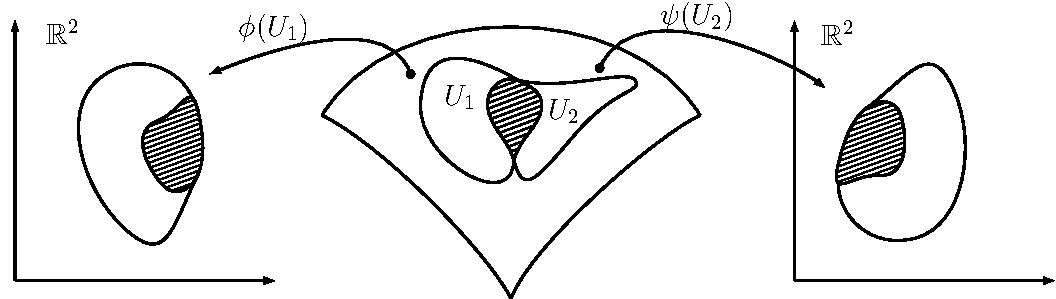
\includegraphics[width=13cm]{figura1.pdf}}          \leyenda{Cartas
    coordenadas usadas en la definici\'on de una variedad topol\'ogica.}
\end{figure}

A  la colecci\'on  de n\'umeros  reales $(p_1  , \ldots  , p_n)$  se  llaman las
coordenadas  de  $p$  de  acuerdo  a  la carta  $(U,\phi)$.   La  existencia  de
coordenadas, es el aspecto fundamental por el que el concepto de variedad es tan
\'util en f\'isica.

Podr\'ia suceder que un mismo punto $p$ pertenezca a m\'as de una carta, digamos
$(U_1,\phi_1)$  y  $(U_2,\psi_2)$.  En  ese  caso  hablaremos  de un  cambio  de
coordenadas:
%
\begin{equation}\label{cc}
\psi \circ \phi^{-1}: \phi(U_1 \cap U_2) \rightarrow \psi(U_1 \cap U_2)
\end{equation}
%
Si denotamos por $(p_1 , \ldots  , p_n)$ a las coordenadas correspondientes a la
carta  $(U_1,\phi_1)$  y  por  $(\tilde{p}_1  , \ldots  ,  \tilde{p}_n)$  a  las
correspondientes a la carta  $(U_2,\psi_2)$, entonces las funciones $\tilde{p}_i
= \tilde{p}_i(p_1 ,  \ldots , p_n)$ son funciones continuas, y  dan el cambio de
coordenadas. Estas funciones son invertibles con inversa continua.

Ejemplos de variedades topol\'ogicas son:
%
\begin{itemize}
\item $\Rset^n$. En este caso hay  una carta coordenada global que cubre toda la
  variedad y donde el homeomorfismo es la identidad.
%
\item $\Sset^n$, la esfera de dimensi\'on $n$. Ella est\'a definida como el conjunto:
  \[
  \Sset^n = \left\{  (x_1 , \ldots ,  x_{n+1}), \: x_i \in \Rset:  \quad x_1^2 +
    \cdots + x_{n+1}^2 = 1 \right\}
  % \text{ tales que }
  \]
\end{itemize}
%
\noindent  Se debe observar  que al  definir $\Sset^n$  no estamos  pensando que
est\'a inmersa  en $\Rset^n$. En este  caso podemos usar  las siguientes cartas:
$(U_N,  \phi_N)$ y $(U_S,\phi_S)$,  donde $U_N  = \Sset^n-\{  (0,0,\ldots,1) \},
\quad U_S = \Sset^n -{(1,0,\ldots,0)}$ y los mapas
%
\[
\phi_N:  U_N  \rightarrow  \Rset^n  /  (\phi_N(x_1  ,  \ldots  ,  n_{n+1}))_i  =
\frac{x_i}{1-x_{n+1}}
\]
%
y
%
\[
\phi_S:  U_S  \rightarrow  \Rset^n  /  (\phi_N(x_1  ,  \ldots  ,  n_{n+1}))_i  =
\frac{x_i}{1+x_{n+1}}
\]
%
Ambos mapas son homeomorfismos.  Observemos  que $\phi_N(x_1 , \ldots , x_{n+1})
= (t x_1 , \ldots , t x_n)$ y  $\phi_S(x_1 , \ldots , x_{n+1}) = (u x_1 , \ldots
,  u  x_n)$   con  $t  =  \frac{1}{1-x_{n+1}}$  y   $u  =  \frac{1}{1+x_{n+1}}$,
respectivamente.  Es directo verificar la  inyectividad pues si $(t x_1 , \ldots
, t x_n) = (t  y_1 , \ldots , t y_n) \Rightarrow x_i =  y_i \quad \forall \: i$.
Entonces  los puntos  $x$  e $y$  son  id\'enticos.  Para  ver la  suryectividad
consideremos el punto  $y = (y_1 , \ldots  , y_n) \in \Rset^n$. Si  tomamos $x =
\left( t^{-1}  y_1 ,  \ldots , t^{-1}  y_n ,  y_{n+1} \right)$ con  $t \ne  0$ e
$y_{n+1} =  t \sqrt{1-(t^{-1}  y_1)^2 - \cdots  - \left( t^{-1}  y_n \right)^2}$
vemos que para cada $y \in \Rset^n$ existe un $x \in \Sset^n$ tal que $\phi(x) =
y$.   Usando las  expresiones  expl\'citas  de $\phi_N$  y  $\phi_S$ es  directo
verificar que se trata de funciones continuas.

{\bf Nota}:  Hay propiedades de las  variedades topol\'ogicas que  no tienen que
ver con sus  caracter\'isticas locales, las que hemos dicho  son similares a las
de  $\Rset^n$,  sino con  sus  propiedades  globales.   Por ejemplo  una  esfera
$2$-dimensional es  homeomorfa a  la superficie de  una pelota de  futbol, a\'un
cuando pensemos en una pelota de futbol verdadera, la cual es una colecci\'on de
parches hexagonales  o pentagonales,  unidos unos con  otros. Ambos  objetos, la
esfera  y la pelota  de futbol,  son objetos  compactos, cerrados  y simplemente
conexos.   Sin  embargo   un  toro  y  una  esfera   no  comparten  todas  estas
caracter\'isticas: un toro  es cerrado, compacto pero no  simplemente conexo, es
decir no  todo lazo sobre  \'el puede contraerse  continuamente a un  punto. Por
ello diremos que un toro y una esfera son localmente homeomorfos, pero no lo son
globalmente. Este tipo de situaciones  ha llevado a introducir cantidades que de
alguna  manera   caractericen  a  las  propiedades  globales   de  una  variedad
topol\'ogicas. Un ejemplo muy conocido  es la caracter\'istica de Euler. Para un
poliedro de  tres dimensiones la  caracteristica de Euler $\Xi$  est\'a definida
por
%
\[
\Xi = V - A + C
\]
%
donde  $V, A$ y  $C$ son  el n\'umero  de vertices,  de aristas  y de  caras del
poliedro, respectivamente. Para un cubo,  por ejemplo, $\Xi = 2$. Supongamos que
el cubo est\'a hecho en un  material el\'astico, apoyado sobre un armaz\'on (las
aristas) de metal. Si inflamos ese cubo, obtenemos una esfera. Matem\'aticamente
eso significa que el cubo y la efera son globalmente homeomorfos entre si, y por
lo  tanto topol\'ogicamente  equivalentes. Es  posible extender  el  concepto de
caracter\'istica  de Euler  a la  superficie  de una  esfera, a  trav\'es de  la
triangularizaci\'on de  la superficie esf\'erica,  es decir cubriendo  la esfera
por tri\'angulos.  En  ese caso la caracter\'istica de Euler  se calcula como el
n\'umero  de tri\'angulos  menos el  n\'umero de  aristas m\'as  el  n\'umero de
v\'ertices. Haci\'endo  ese c\'alculo  para la esfera  resulta el valor  $2$. Lo
mismo sucede con cualquier otro poliedro que se pueda deformarse continuamente a
una  esfera.  Hay maneras  de  definir la  caracter\'istica  de  Euler para  una
variedad topol\'ogica  arbitraria y esa cantidad es  un invariante topol\'ogico,
es decir  una cantidad que no  cambia entre variedades  homeom\'orficos. Para un
toro la caracter\'istica de Euler vale $0$.


% =========================== Variedad Diferenciable ========================= %

%\sub
\seccion{Variedad Diferenciable}
\label{s:WL:VariedadDiferenciable}

Sobre una  variedad topol\'ogica  se puede ``montar''  una nueva  estructura. Es
posible  hacer  eso imponiendo  condiciones  de  diferenciabilidad  a los  mapas
coordenados de  la definici\'on  de una variedad  topol\'ogica. Sin  embargo, no
tenemos   definida  la   noci\'on   de  diferenciablidad   sobre  una   variedad
cualquiera.  Por  ello, para  definir  una  estructura  diferenciable sobre  una
variedad  topol\'ogica  arbitraria,  recurrimos  a  $\Rset^n$  donde  si  est\'a
definida la noci\'on de diferenciabilidad. Por ello hacemos la siguiente:
%
\begin{definicion}[$C^r$-compatibilidad]
  Diremos que dos cartas coordenadas  $(U,\phi)$ y $(V,\psi)$ sobre una variedad
  $\M$ son  $C^r$-compatibles si  cuando $U \bigcap  V \ne \emptyset  $ entonces
  $\phi \circ \psi^{-1}$  y $\psi \circ \phi^{-1}$ son de  clase $C^r$ sobre los
  subconjuntos  $\phi(U  \bigcap  V)$   y  $\psi(U  \bigcap  V)$  de  $\Rset^n$,
  respectivamente.
\end{definicion}
%
Con esto podemos avanzar en la siguiente:
%
\begin{definicion}[Variedad diferenciable]
  Una {\it Variedad diferenciable} $n$-dimensional  de clase $C^r$, $\M$, es una
  variedad  topol\'ogica  y una  familia  de  cartas  coordenadas $\B  =  \left(
    U_\alpha , \phi_\alpha \right)$, tales que:
  %
  \begin{enumerate}
  \item los $U_{\alpha}$ cubren $\M$,
  %
  \item  para cualquier  par $\alpha,  \beta$, los  entornos $\left(  U_\alpha ,
      \phi_\alpha \right)$  y $\left( U_\beta  , \phi_\beta \right)$  son $C^r$-
    compatibles,
  %
  \item  Cualquier   entorno  coordenado  $(V,\psi)   \:\:  C^r$-compatible  con
    cualquiera de los  $\left( U_\alpha , \phi_\alpha \right)  \in \B$ est\'a en
    $\B$.
  \end{enumerate}
\end{definicion}

\begin{figure}
 \centerline{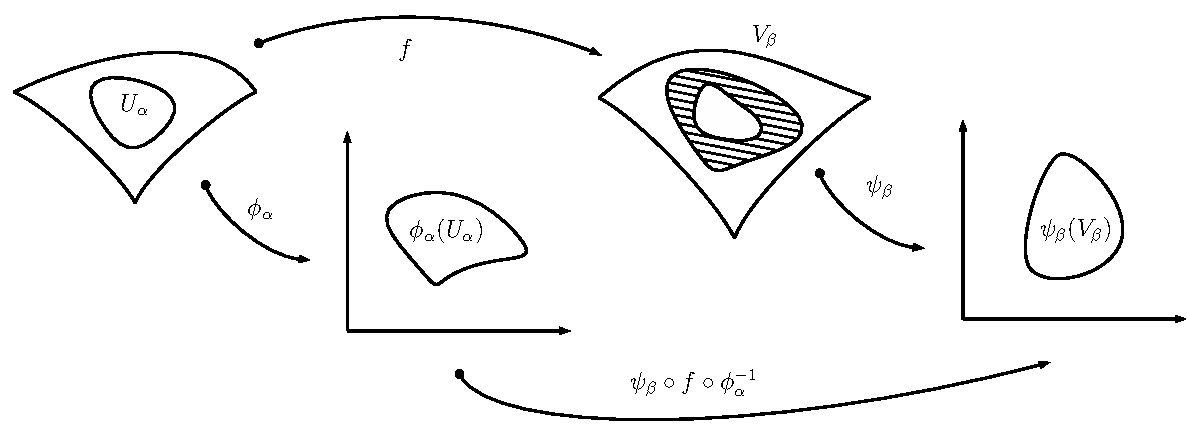
\includegraphics[width=13cm]{figura2.pdf}}
%
 \leyenda{Cartas  coordenadas  usadas  en   la  definici\'on  de  una  funci\'on
   diferenciable.}
\end{figure}

Cualquier  superficie ``suave''  en $\Rset^3$  es un  ejemplo de  (sub) variedad
diferenciable. Este ejemplo no debe conducir  a la confusi\'on de pensar que una
variedad debe estar inmersa en $\Rset^n$. Otro ejemplo de variedad diferenciable
de dimensi\'on $n$ es la esfera $\Sset^n$, definida previamente.

\begin{definicion}[Diferenciabilidad de clase $C^k$]
  Dadas  dos variedades  $\M$ y  $\M'$ de  clase $C^r$,  una  aplicaci\'on $f:\M
  \rightarrow \M' $,  se dice {\it diferenciable} de clase $C^k,  \quad k \le r$
  si para  toda carta  $\left( U_\alpha  , \phi_\alpha \right)$  de $\M$  y toda
  carta  de $\left(  V_\beta ,  \psi_\beta \right)$  de $\M'$  tal  que $f\left(
    U_\alpha \right) \subset V_\beta$, la aplicaci\'on $\psi_\beta \circ f \circ
  \phi_\alpha^{-1}$ de $\phi_\alpha\left( U_\alpha \right)$ en $\psi_\beta\left(
    V_\beta \right)$, es diferenciable de clase $C^k$.
\end{definicion}

El disponer  de la noci\'on de  funci\'on diferenciable, permite  asignar a cada
punto de una variedad diferenciable,  un espacio vectorial. \'Este estar\'a dado
por operadores  lineales que act\'uan  sobre funciones diferenciables y  dan por
resultado un n\'umero.  Antes de ir a la definici\'on  de ese espacio vectorial,
introducimos el concepto de curva suave sobre una variedad.
%
\begin{definicion}[Curva de clase $C^k$ sobre una variedad]
  Sea $\M$  una variedad de  clase $C^r$. Una  curva $\lambda$ en $\M$  de clase
  $C^k, \quad k  \le r$ es una funci\'on  del intervalo real $[a \, ,  \, b]$ en
  $\M$ tal que  para toda carta $\left( U_\alpha ,  \phi_\alpha \right)$ en $\M$
  la composici\'on
  %
  \[
  \phi_\alpha \circ \gamma: [a \, , \, b] \rightarrow \phi_\alpha\left( U_\alpha
  \right)
  \]
  %
  es de clase $C^k$. En coordenadas
  %
  \[
  \phi_\alpha \circ \gamma (t) = \{ x^1(t) , \ldots , x^n(t) \}
  \]
\end{definicion}
%
Con esto podemos ahora dar la noci\'on de vector tangente a una variedad:
%
\begin{definicion}[Tangente a una variedad]
  Sea $\F(p)$ el  conjunto de funciones diferenciables de  clase $C^1$ definidas
  en un entorno del punto $p$.  Sea $\gamma(t)$ una curva de clase $C^1$, $a \le
  t  \le b$  tal que  $\gamma(t_0) =  p$. El  vector {\it  tangente} a  la curva
  $\gamma(t)$ en el punto $p$ es una aplicaci\'on $\mathbb{X}_p : \F(p) \rightarrow \Rset$
  % \[
  % \mathbb{X}_p : \F(p) \rightarrow \Rset
  % \]
  cuyo efecto es
  %
  \[
  \mathbb{X}_p f = \frac{df(\gamma (t))}{dt} |_{t_0}
  \]
\end{definicion}
%
El vector $\mathbb{X}_p$ satisface las siguientes propiedades
%
\begin{itemize}
 \item $\mathbb{X}_p$ es una aplicaci\'on lineal de $\F(p)$ en $\Rset$,
  %
 \item  $\mathbb{X}_p(fg) =  \left( \mathbb{X}_p  f \right)  g(p) +  f(p) \left(
     \mathbb{X}_p g \right)$ para $f , g \in \F(p)$.
\end{itemize}
%
Dejamos para el lector demostrar estas propiedades.

Sean $(u^1 , \ldots  , u^n)$ coordenadas locales en un entorno  $U$ de $p$. Para
cada $j$, $\left( \frac{\partial}{\partial  u^j} \right)|_p$ es una aplicaci\'on
de $\F(p)$  en $\Rset$ la cual satisface  las propiedades (i) e  (ii). Veremos a
continuaci\'on que el conjunto de todas las aplicaciones $\mathbb{X}$ de $\F(p)$
en $\Rset$ es un espacio vectorial $n$-dimensional, siendo $n$ la dimensi\'on de
la variedad diferenciable $\M$.

Dada una  curva $\gamma(t)$ con $\gamma(t_0)  = p$, sean  $u^j(t) = \gamma^j(t),
\quad  j =  1 ,  \ldots ,  n$  las coordenadas  locales de  esa curva.  Entonces
$\frac{df(\gamma(t))}{dt}|_{t_0}  =  \sum_j  \left(  \frac{\partial  f}{\partial
    u^j}|_p  \right)  \left( \frac{d  \gamma^j  (t)}{dt} \right)|_{t_0}$.  Extra %% ESTA???
expresi\'on indica  que todo vector  en $p$ es  una combinaci\'on lineal  de los
vectores (operadores).

\begin{equation}
\left(\frac{\partial}{\partial u^1}|_p \right),\ldots,\left(\frac{\partial}{\partial u^n}|_p \right) \label{set}
\end{equation}

Sea la  combinaci\'on lineal  $\sum_j \xi^j \frac{\partial}{\partial  u^j}|_p$ y
sea la curva definida por
%
\[
u^j(t) = u^j(p) + \xi^j t \quad j = 1 , \ldots , n
\]
%
El   vector   tangente   a   esta   curva   en  $t   =   0$   es   $\sum   \xi^j
\frac{\partial}{\partial u^j}|_p$.  Adem\'as si
%
\[
\sum \xi^j \frac{\partial}{\partial u^j}|_p =0,
\]
%
entonces
%
\[
0 = \sum \xi^j \left( \frac{\partial u^k}{\partial u^j} \right)|_p = \xi^k \quad
k = 1 , \ldots , n
\]
%
Esto demuestra la independencia lineal de los vectores~\eqref{set}.
%
\begin{definicion}[Espacio tangente]
  El conjunto  de vectores tangentes en $p  \in \M$, es llamado  el {\it espacio
    tangente de $\M$ en $p$}, y lo denotaremos por $T_p(\M)$.
\end{definicion}

La colecci\'on de todos los  espacios tangentes, $\bigcup_{p \in \M} T_p(\M)$ se
llama {\it fibrado tangente}.

Al fibrado tangente se le puede  dar la estructura de un \'algebra (\'algebra de
Lie). Esta surge de calcular  el conmutador $[\mathbb{X}, \mathbb{Y}]$ entre dos
campos vectoriales $\mathbb{X}$ e $\mathbb{Y}$:
%
\[
[\mathbb{X},  \mathbb{Y}] f  \equiv  \left( \mathbb{X}  \mathbb{Y} -  \mathbb{Y}
  \mathbb{X} \right) f
\]
%
Si los vectores  se escriben en t\'ermino de los vectores  de la base coordenada
$\left(  \frac{\partial}{\partial  x^a}  \right)$,  el  conmutador  entre  ellos
resulta ser el vector:
%
\[
\sum_{ab} X^a \frac{\partial  Y^b}{\partial x^a} \frac{\partial}{\partial x^b} -
\sum_{ab} Y^a \frac{\partial X^b}{\partial x^a} \frac{\partial}{\partial x^b}
\]

A cada espacio tangente $T_p(\M)$ podemos asignar su dual, $T_p^*(\M)$, es decir
el conjunto de  todos los operadores lineales y  homog\'eneos que act\'uan sobre
$T_p(\M)$.   A    un   elemento   del   espacio   dual    lo   llamaremos   {\it
  $1$-forma}. Denotaremos a  la acci\'on de un elemento  de $T_p^*(\M)$, digamos
$\omega_p$, por:
%
\[
\omega_p(\mathbb{X}_p) = \left\langle \omega_p , \mathbb{X}_p \right\rangle.
\]
%
Para cada  funci\'on $f \in  \F(p)$, el {\it  diferencial de $f$},  denotado por
$(df)_p$, es el elemento de $T_p^*(\M)$ que tiene por acci\'on:
%
\[
\left\langle (df)_p ,  \mathbb{X}_p \right\rangle = \mathbb{X}_p f,  \quad \mathbb{X}_p \in
T_p(\M)
\]

Cada funci\'on coordenada $u^j$ es una funci\'on de $\M$ sobre $\Rset$. Entonces
podemos  calcular  el  diferencial  de  $u^j$, cuya  acci\'on  sobre  un  vector
$\mathbb{X}_p \in T_p(\M)$ est\'a dada por
%
\[
 \left\langle (du^j)_p , \mathbb{X}_p \right\rangle = \mathbb{X}_p^j
\]
%
En particular,  si $\mathbb{X}_p =  \left(\frac{\partial}{\partial u^k} \right)$
resulta
%
\[
\left\langle   (du^j)_p   ,   \left(   \frac{\partial}{\partial   u^k}   \right)
\right\rangle = \delta_k^j;
 \]
%
 es decir $\left\{ (du^j)_p \right\}_{j=1}^n$ es la base dual de $\left\{ \left(
     \frac{\partial}{\partial  u^j} \right)_p \right\}_{j=1}^n$.  Toda $1$-forma
 $\omega$ se puede escribir en t\'ermino de esta base:
%
\[
\omega = \sum_a \omega_a dx^a
\]

Con los espacios  $T_p(\M)$ y $T_p^*(\M)$ podemos construir  el espacio producto
cartesiano
%
\[
\left(  T_p(\M)  \right)_s^r =  T_p(\M)  \times  T_p(\M)  \ldots T_p(\M)  \times
T_p^*(\M) \times T_p^*(\M) \ldots \times T_p^*(\M)
\]
%
con $r$ factores de $T_p(\M)$ y $s$ factores de $T_p^*(\M)$.

\begin{definicion}[Tensor de tipo $(r,s)$]
  Un {\it tensor de tipo $(r,s)$} es un operador $S$,
  %
  \[
  S: \left( T_p(\M) \right)_s^r \rightarrow \Rset
  \]
  %
  que es lineal y homog\'eneo en cada uno de sus argumentos.
\end{definicion}

\begin{definicion}[Campo tensorial]
  Un {\it campo tensorial $S$ de  clase $C^k$ de tipo $(r,s)$ sobre $V \subseteq
    \M$} es un mapa  $C^k$ que asigna un tensor de tipo  $(r,s)$ a cada punto $p
  \in V$.
\end{definicion}
%
En  t\'ermino  de las  bases  $\left\{  \left( \frac{\partial}{\partial  u^j}|_p
  \right)  \right\}_{j=1}^n$  y $\left\{  (du^j)_p  \right\}_{j=1}^n$, el  campo
tensorial $S$ se puede escribir:
%
\[
S(p) = S^{a_1 \ldots  a_r}_{b_1 \ldots b_s}(p) \frac{\partial}{\partial x^{a_1}}
\bigotimes   \ldots  \bigotimes  \frac{\partial}{\partial   x^{a_r}}  \bigotimes
dx^{b_1} \bigotimes \ldots \bigotimes dx^{b_s}
\]
%
\noindent donde  las funciones $S^{a_1 \ldots a_r}_{b_1 \ldots b_s}$  son de clase
$C^k$ y $\bigotimes$ es el producto tensorial.

Entre los campos tensoriales que se  pueden definir sobre una variedad $\M$, hay
uno particularmente importante,  y es conocido como el  tensor m\'etrico. \'Este
se define por medio de un producto escalar:
%
\begin{definicion}[Producto escalar]
  Un {\bf producto escalar} sobre $T_p(\M)$ es una funci\'on
  %
  \[
  g: T_p(\M) \times T_p(\M) \rightarrow \Rset
  \]
  %
  que satisface
  %
  \begin{enumerate}
  \item $g(\mathbb{X}, \mathbb{Y}) = g(\mathbb{Y}, \mathbb{X}), \quad \text{para}
    \quad \mathbb{X}, \mathbb{Y} \in T_p(\M)$
  %
  \item  $g(\mathbb{X},   a  \mathbb{Y}  +  b  \mathbb{Z})   =  a  g(\mathbb{X},
    \mathbb{Y}) + b g(\mathbb{X}, \mathbb{Z})$
  \end{enumerate}
\end{definicion}

El producto escalar se dice  {\it no degenerado} si $g(\mathbb{X}, \mathbb{Y})=0
\quad \forall \:  \mathbb{Y} \in T_p(\M)$ implica $\mathbb{X}  = 0$.  Obviamente
el  producto  escalar  es un  tensor  de  tipo  $(0,2)$.  Como  campo  tensorial
$g(\;,\;)$   se   puede   expresar    en   t\'erminos   de   la   base   $\left(
  \frac{\partial}{\partial    u^1}|_p     \right)    ,    \ldots     ,    \left(
  \frac{\partial}{\partial u^n}|_p \right)$
%
\[
g(\mathbb{X}, \mathbb{Y})  = \sum_{ab} X^a  Y^b g\left( \frac{\partial}{\partial
    u^a}, \frac{\partial}{\partial u^b} \right)
\]
%
o, de manera equivalente
%
\[
g(\mathbb{X}, \mathbb{Y}) = \sum_{ab} g_{ab} X^a Y^b
\]
%
donde     $g_{ab}    =    g     \left(    \frac{\partial}{\partial     u^a}    ,
  \frac{\partial}{\partial  u^b}   \right)$.  Si  el  producto   escalar  es  no
degenerado, entonces  existe la  matriz inversa de  la matriz $g_{ab}$,  a cuyos
elementos los denotaremos por $g^{ab}$, de modo que
%
\[
\sum_c g_{ac} g^{cb} = \delta_a^b
\]

La  existencia de  un campo  tensorial  m\'etrico (o  producto escalar  definido
localmente),  permite introducir  la idea  de {\it  longitud de  una  curva}. En
efecto, sea  $\gamma(t), \quad t  \in [a \,  , \, b]$  una curva de  clase $C^1$
sobre $\M$,  que une los  puntos $p$  y $q$: $\gamma(a)  = p, \quad  \gamma(b) =
q$. En el punto $\gamma(t)$ tenemos  el vector tangente a la curva $\gamma$ dado
por
%
\[
\left( \frac{\partial}{\partial t} \right)_\gamma = \sum_j \frac{d \gamma^j}{dt}
\frac{\partial}{\partial x^j}
\]

\begin{definicion}[Longitud de una curva]
  La {\it longitud de la curva $\gamma$  entre los puntos $p$ y $q$} est\'a dada
  por la cantidad
  %
  \begin{equation}
    L = \int_a^b | g \left( \frac{\partial}{\partial t}, \frac{\partial}{\partial t} \right) |^{\frac{1}{2}} dt
  \label{longitud}
  \end{equation}
\end{definicion}
%
O, equivalentemente
%
\begin{equation}
L = \int_a^b \left| \sum_{ij} g_{ij}(x) \frac{d\gamma^i}{dt} \frac{d \gamma^j
}{dt} \right|^{\frac{1}{2}} dt \label{longitud}
\end{equation}

% ============================== Estructura Afin ============================= %

%\sub
\seccion{Estructura Afin}
\label{s:WL:EstructuraAfin}

En  el espacio  eucl\'ideo  $n$-dimensional (pensado  aqu\'i  como una  variedad
diferenciable),  cuando  usamos coordenadas  cartesianas,  caracterizamos a  dos
vectors paralelos como aquellos  que tienen iguales componentes. Si reemplazamos
las coordenadas cartesianas por las polares, por ejemplo, esta caracterizaci\'on
deja  de  ser  v\'alida.  Veamos   c\'omo  podemos  introducir  la  noci\'on  de
paralelismo de vectores, usando  cualquier sistema de coordenadas. Sea $\{x^a\}$
el sistema de  coordenadas cartesiano del espacio. En  este sistema, hemos dicho
que  dos vectores  paralelos,  por ejemplo  $\mathbb{V}$ y  $\tilde{\mathbb{V}}$
tienen iguales componentes:
%
\[
V^a = \tilde{V}^a
\]
%
Si el vector $\mathbb{V}$ es tangente al espacio en el punto $p$ con coordenadas
$\{ x^a \}$  y el vector paralelo $\tilde{\mathbb{V}}$ es  tangente al punto $q$
con coordenadas ${x^a+\delta x^a}$, vale
%
\[
\tilde{V}^a(q)-V^a(p) = 0
\]
%
Dado  un  vector $\mathbb{V}$  en  $p$, podemos  definir  un  campo de  vectores
paralelos  a $\mathbb{V}$  en un  entorno  de $p$.  Denotemos a  este campo  por
$\tilde{\mathbb{V}}$.  Este  campo cumple  que  en  el  punto $p$  coincide  con
$\mathbb{V}$ y con la condici\'on:
%
\[
\tilde{V}^a(x+\delta x) -  V^a(x) = \frac{\partial \tilde{V}^a}{\partial x^b}(p)
\delta x^b
\]
%
Sea ${\xi^a}$ otro sistema de  coordenadas para el espacio eucl\'ideo, vinculado
con ${x^a}$ mediante las relaciones
%
\begin{equation}
\xi^a = \xi^a(x^b), \quad x^b=x^b(\xi^a) \label{cambcoor}
\end{equation}
%
A partir de ellas, resulta
%
\begin{equation}
\delta \xi^a = \frac{\partial \xi^a}{\partial x^b} \delta x^b, \qquad \delta x^b = \frac{\partial x^b}{\partial \xi^a} \delta \xi^a
\end{equation}
%
Las componentes de $\tilde{\mathbb{V}}$ se transforman de acuerdo con
%
\[
\tilde{V}^a = \frac{\partial x^a}{\partial \xi^b} \tilde{V'}^b
\]
%
donde  $\tilde{V'}^a$  son  las   componentes  de  $\tilde{\mathbb{V}}$  en  las
coordenadas $\{\xi^a\}$. Entonces, podemos escribir
%
\begin{eqnarray}
\frac{\partial \tilde{V}^a}{\partial x^b} &=& \frac{\partial}{\partial \xi^c} \left(\frac{\partial x^a}{\partial \xi^d} \tilde{V'}^d \right) \frac{\partial \xi^c}{\partial x^b}  \nonumber \\
%
& = & \frac{\partial^2 x^a}{\partial \xi^c \partial \xi^d} \tilde{V'}^d \frac{\partial \xi^c}{\partial x^a}+ \frac{\partial x^a}{\partial \xi^d} \frac{\partial{\tilde{V'}^d}}{\partial \xi^c} \frac{\partial \xi^c}{\partial x^b}
\end{eqnarray}
%
Si    definimos   la    cantidad   $\delta    \tilde{V'}^d    =   \frac{\partial
  \tilde{V'}^d}{\partial x^e} \delta \xi^e$ y despu\'es de un poco de \'algebra,
llegamos a la relaci\'on
%
\begin{equation}
\delta \tilde{V'}^n = - \frac{\partial^2 x^a}{\partial \xi^e \partial \xi^d} \frac{\partial \xi^n}{\partial x^a} \tilde{V'}^d \delta \xi^e \label{con}
\end{equation}
%
Esta expresi\'on puede reescribirse de la siguiente forma:
%
\begin{equation}
\delta \tilde{V'}^n = - \Gamma'^n_{ed} \tilde{V'}^d \delta \xi^e
\end{equation}
%
\noindent  en   donde  los  coeficientes  $\Gamma'$  est\'an   definidos  en  la
expresi\'on~\eqref{con}. De su definici\'on resulta que las cantidades $\Gamma'$
se anulan para cambios {\it lineales} de coordenadas~\eqref{cambcoor}.

Obs\'ervese que al haber arribado a la definici\'on de los coeficientes $\Gamma$
no hemos hecho uso de ninguna  propiedad especial del espacio eucl\'ideo. Es por
ello  que  la  expresi\'on~\eqref{con}   es  v\'alida  para  cualquier  variedad
n-dimensional. Es f\'acil ver que frente a un cambio de coordenadas
%
\begin{equation}
x^a \rightarrow x'^a= x'^a\left(x^b\right) \label{camb2}
\end{equation}
%
las cantidades $\Gamma$ cambian seg\'un la expresi\'on
%
\begin{equation}
\Gamma ^f_{de} = \Gamma'^a_{mn} \frac{\partial x^f}{\partial x'^a} \frac{\partial x'^m}{\partial x^d} \frac{\partial x'^n}{\partial x^e}+\frac{\partial x^f}{\partial x'^a} \frac{\partial^2 x'^a}{\partial x^e \partial x^d} \label{camcon}
\end{equation}
%
Debemos  remarcar que  esta  ley  de transformaci\'on  es  lineal y  homog\'enea
(tensorial)   s\'olo  cuando  el   cambio  de   coordenadas~\eqref{cambcoor}  es
lineal. Esta propiedad  de los coeficientes $\Gamma$ nos  permite generalizar la
idea de paralelismo en una variedad arbitraria:
%
\begin{definicion}[Conexi\'on af\'in]
  Cuando  en una  variedad  n-dimensional arbitraria  $\M$  se introducen  $n^3$
  coeficientes $\Gamma$ que se transforman de acuerdo con la ley~\eqref{camcon},
  diremos que sobre esa variedad se ha definido una {\it conexi\'on af\'in}
\end{definicion}

A partir de los coeficientes $\Gamma$ es posible definir una nueva derivada para
un campo vectorial arbitrario, digamos $V^a(x)$:
%
\begin{definicion}[Derivada covariante de campo]
  Sea  un campo vectorial  $V$ definido  en un  entorno del  punto $x$.  La {\it
    derivada covariante  del campo  $V$} est\'a dado  por las componentes  de un
  tensor de tipo $(1,1)$
  %
  \[
  V^a_{;c} = V^a_{,c} + \Gamma^a_{bc} V^b
  \]
\end{definicion}

\begin{definicion}[Derivada covariante en una direcci\'on]
  Dados dos campos  vectoriales $U(x)$ y $V(x)$, la  {\it derivada covariante de
    $V$ en la direcci\'on de $U$} es el campo vectorial definido por
  %
  \[
  U(x) \cdot \nabla V(x) \equiv \sum_{ab} V^a_{;b}(x) U^b(x) \mathbb{E}_a \equiv
  \nabla_U V
  \]
% hdot => cdot?
\end{definicion}
%
donde  $\mathbb{E}^a$ es  el campo  de  vectores coordenados  asociados con  las
coordenadas $x^a$. Esta \'ultima  definici\'on permite trasladar paralelamente a
un vector a  lo largo de una  curva. Basta con tomar como  $\mathbb{U}$ al campo
tangente a la curva.


% ============================== Variedad Riemanniana ============================= %

%\sub
\seccion{Variedad Riemmanniana}
\label{s:WL:VariedadRiemmanniana}

Sea $\M$ una variedad diferenciable  $n$-dimensional. Si $\M$ tiene definida una
m\'etrica  no   singular  sobre  ella,   recibe  el  nombre  de   {\it  variedad
  Riemanniana}. La existencia de una m\'etrica sobre $\M$ permite introducir una
conexi\'on af\'in  particular, conocida como la conexi\'on  de Levi-Civita. Sean
$g_{ab}$ y  $g^{ab}$ los coeficientes de la  m\'etrica $g$ y su  inversa, en las
coordenadas $\{x^a\}$, respectivamente.

Para  dos puntos  pr\'oximos,  la separaci\'on  entre  ellos viene  dada por  la
expresi\'on:
%
\begin{equation}
ds^2 = \sum_{ab} g_{ab} dx^a dx^b \label{quad}
\end{equation}

Adem\'as de definir una distancia  entre puntos pr\'oximos, la existencia de una
m\'etrica  permite   definir  una  conexi\'on  particular   sobre  una  variedad
riemanniana:
%
\begin{definicion}[Conexi\'on de Levi-Civita]
  La conexi\'on de Levi-Civita en las coordenadas $x^a$ est\'a dada por:
  %
  \begin{equation}
  \Gamma^a_{bc} = \frac{1}{2} \sum_d g^{ad} \left(g_{bd,c} + g_{cd.b} - g_{bc.d} \right) \label{levi}
  \end{equation}
\end{definicion}

La existencia  de esta  particular conexi\'on no  imposibilita la  existencia de
otras conexiones definidas sobre $\M$.

Como hemos visto  m\'as arriba, el tener definida  una m\'etrica permite definir
la  longitud de  una curva.  Bajo ciertas  condiciones, que  supondremos  que se
satisfacen, podemos plantearnos el problema  de determinar la curva que minimiza
(en  realidad  extremiza)  su  longitud  al  unir  dos  puntos  fijos  sobre  la
variedad. Esto se puede tratar  resolviendo el problema variacional asociado con
el funcional~\eqref{longitud}. La ecuaci\'on de Euler-Lagrange  conduce en este
caso a:
%
\begin{equation}
\frac{d^2 x^d}{dt^2} + \Gamma^d_{ca} \frac{dx^c}{dt} \frac{dx^a}{dt} = 0 \label{geode}
\end{equation}
%
\noindent donde $x^a(t)$ son las coordenadas de la curva y $t$ es un par\'ametro
adecuadamente elegido. Una curva  que satisface~\eqref{geode}, se llama una {\it
  curva geod\'esica}.  Es posible caracterizar  a una curva geod\'esica  de otro
modo. Sea  $\mathbb{U}(t)$ el vector  tangente a una curva  $\gamma(t)$ definida
sobre $\M$.  La curva $\gamma$ se  dice una geod\'esica si su vector tangente es
trasladado paralelamente a lo largo de ella:
%
\[
\mathbb{U} \cdot \nabla \mathbb{U} = f(t) \mathbb{U}
\]
% 
% hdot => cdot?
Siempre es posible  elegir al par\'ametro $t$ de forma tal  que $f(t)=0$, con lo
cual reobtenemos la ecuaci\'on~\eqref{geode}.

El disponer de geod\'esicas, permite dar a una variedad riemanniana el car\'cter
de espacio m\'etrico.  En efecto, podemos definir la  distancia entre dos puntos
$p$ y $q$ de la variedad $\M$ a trav\'es de la expresi\'on:
%
\begin{equation}
d(p,q) = \min_{\gamma} L(\gamma) \label{distt}
\end{equation}
%
\noindent donde  el m\'inimo  se eval\'ua  entre todas las  curvas que  unen los
puntos $p$ y $q$, y $L$ es la longitud~\eqref{longitud}. Como siempre, todo esto
es  posible ser  realizado  localmente.   Las geod\'esicas  son  las curvas  que
localmente  minimizan  la distancia  entre  dos  puntos.  La distancia  definida
por~\eqref{distt}  verifica  la  desigualdad   triangular,  y  por  eso  es  una
m\'etrica.

Dada una conexi\'on  $\nabla$ se define un tensor de  tipo $(1,3)$, llamado {\it
  tensor de curvatura} asociado a la conexi\'on $\nabla$, cuya espresi\'on es:
%
\[
\R\left( \mathbb{X} , \mathbb{Y} \right) \mathbb{Z} = \nabla_{\mathbb{X}} \left(
  \nabla_{\mathbb{Y}}   \mathbb{Z}    \right)   -   \nabla_{\mathbb{Y}}   \left(
  \nabla_{\mathbb{X}}  \mathbb{Z}   \right)  -  \nabla_{[\mathbb{X},\mathbb{Y}]}
\mathbb{Z}
\]
%
Si los  vectores $\mathbb{X}$, $\mathbb{Y}$ y $\mathbb{Z}$  son reemplazados por
los       vectors       coordenados       $\frac{\partial}{\partial       x^a}$,
$\frac{\partial}{\partial     x^b}$    y     $\frac{\partial}{\partial    x^c}$,
respectivamente, resulta
%
\[
\R\left( \frac{\partial}{\partial  x^a} , \frac{\partial}{\partial  x^b} \right)
\frac{\partial}{\partial x^c} = R^d_{cab} \frac{\partial}{\partial x^d}
\]
%
con
%
\[
R^d_{cba}   \equiv  \left(  \frac{   \partial  \Gamma^d_{cb}}{\partial   x^a}  +
  \Gamma^d_{ra} \Gamma^r_{cb}  - \frac{ \partial  \Gamma^d_{ca}}{\partial x^b} -
  \Gamma^d_{rb} \Gamma^r_{ca}\right) \frac{\partial}{\partial x^d}
\]

{\bf  Nota:} Si  bien existe  una motivaci\'on  geom\'etrica para  introducir el
tensor de curvatura, aqu\'i no la hemos  dado. Ella tiene que ver con la idea de
cu\'anto cambia un  vector al desplazarlo paralelamente a lo  largo de una curva
cerrada. En general diremos que una  variedad es plana, si todas las componentes
de su tensor de curvatura, se anulan.

Concluimos  este cap\'itulo  con una  breve  nota hist\'orica.  En sus  trabajos
originales sobre geometr\'ia, B. Riemann  introdujo el elemento de l\'inea entre
dos puntos vecinos $p$ y $q$ por medio de la expresi\'on
\begin{equation}
ds = F(p, \mathbb{X})dt \label{linea}
\end{equation}
%
con $F(  p , \mathbb{X} )$  una funci\'on homog\'enea  de grado 2 en  la segunda
variable. Aqu\'i estamos suponiendo que  los puntos $p$ y $q$ tienen coordenadas
${x^a}$  y ${x^a +  X^a dt}$,  respectivamente. La  geometr\'ia basada  sobre el
elemento de l\'inea  se conoce como geometr\'ia de  Finsler.  Obs\'ervese que el
elemento~\eqref{quad} (de  Riemann) es un  caso particular de la  geometr\'ia de
Finsler.

 % Walter/Mariela
{\color{red}\bf CF libro de Bullet et al.~\cite{BulFea17}, Cencov~\cite{Cen82}, Amari~\cite{AmaNag00}.}
%\capitulo{Geometr\'ia de la informaci\'on}{}


% Epigrafe de capitulo
\begin{epigrafe}
  \textcolor{red}{Esto es  un ep\'igrafe con  texto simulado.\\ Esto es  un ep\'grafe
    con  texto simulado.
\autortituloepigrafe{Autor del ep\'igrafe, T\'itulo de la obra}
}
\end{epigrafe}


\seccion{La Secci\'on 4.1}
\label{s:4.1}

Este es un  p\'arrafo Normal con texto simulado, (Arial  10, interlineado de 1,5
l\'ineas, sangr\'ia en primera l\'inea de 0,5cm. Este es un p\'arrafo Normal con
texto simulado,  (Arial 10, interlineado  de 1,5 l\'ineas, sangr\'ia  en primera
l\'inea de 0,5cm). Este es un  p\'arrafo Normal con texto simula- do, (Arial 10,
interlineado de 1,5 l\'ineas, sangr\'ia en primera l\'inea de 0,5cm). Este es un
p\'arrafo Normal  con texto simulado,  (Arial 10, interlineado de  1,5 l\'ineas,
sangr\'ia en primera  l\'inea de 0,5cm).  Este es un  p\'arrafo Normal con texto
simulado, (Arial 10, interlineado de  1,5 l\'ineas, sangr\'ia en primera l\'inea
de 0,5cm)\notaalpie{Eso es una footnote sobre varias lineas. Eso es una footnote
  sobre varias  lineas.  Eso  es una  footnote sobre varias  lineas. Eso  es una
  footnote sobre varias lineas. Eso es  una footnote sobre varias lineas. Eso es
  una footnote sobre varias lineas. Eso es una footnote sobre varias lineas. Eso
  es  una  footnote  sobre varias  lineas.  Eso  es  una footnote  sobre  varias
  lineas. Eso es una footnote sobre varias lineas.}.

% citas (de mas de 40 palabras)) ==============================================
\begin{citas}
  {\color{red} Esto  es un ejemplo  de cita  de mas de  40 palabras. Esto  es un
    ejemplo de cita de mas de 40 palabras.  Esto es un ejemplo de cita de mas de
    40 palabras. Esto  es un ejemplo de cita  de mas de 40 palabras.  Esto es un
    ejemplo de cita de mas de 40 palabras.}
\end{citas}

Este es un  p\'arrafo Normal con texto simulado, (Arial  10, interlineado de 1,5
l\'ineas, sangr\'ia en primera l\'inea de 0,5cm. Este es un p\'arrafo Normal con
texto simulado,  (Arial 10, interlineado  de 1,5 l\'ineas, sangr\'ia  en primera
l\'inea de 0,5cm). Este es un  p\'arrafo Normal con texto simula- do, (Arial 10,
interlineado de 1,5 l\'ineas, sangr\'ia en primera l\'inea de 0,5cm). Este es un
p\'arrafo Normal  con texto simulado,  (Arial 10, interlineado de  1,5 l\'ineas,
sangr\'ia en  primera l\'inea de 0,5cm).  Este es un p\'arrafo  Normal con texto
simulado, (Arial 10, interlineado de  1,5 l\'ineas, sangr\'ia en primera l\'inea
de 0,5cm).

\begin{figure}[h!]
\centerline{
\includegraphics[width=2cm]{logo_large}}
%
\leyenda{Eso es  una figura, con  su leyenda sobre  varias lineas para  ver como
  queda en el texto. Eso es una  figura, con su leyenda sobre varias lineas para
  ver como queda en el texto.}
\end{figure}

Este es un  p\'arrafo Normal con texto simulado, (Arial  10, interlineado de 1,5
l\'ineas, sangr\'ia en primera l\'inea de 0,5cm. Este es un p\'arrafo Normal con
texto simulado,  (Arial 10, interlineado  de 1,5 l\'ineas, sangr\'ia  en primera
l\'inea de 0,5cm). Este es un  p\'arrafo Normal con texto simula- do, (Arial 10,
interlineado de 1,5 l\'ineas, sangr\'ia en primera l\'inea de 0,5cm). Este es un
p\'arrafo Normal  con texto simulado,  (Arial 10, interlineado de  1,5 l\'ineas,
sangr\'ia en  primera l\'inea de 0,5cm).  Este es un p\'arrafo  Normal con texto
simulado, (Arial 10, interlineado de  1,5 l\'ineas, sangr\'ia en primera l\'inea
de 0,5cm).

\begin{table}
\leyenda{Eso es un ejemplo de tabla}
\begin{center}
\begin{tabular}{|c|c|c|}
\hline
{\bf T\'itulo (negrita)} & {\bf T\'itulo (negrita)} & {\bf T\'itulo (negrita)}\\
\hline
A & Texto simulado (normal) & Texto simulado (normal)\\
\hline
B & Texto simulado (normal) & Texto simulado (normal)\\
\hline
\end{tabular}
\fuente{Eso ser\'ia el fuente de la tabla}
\end{center}\end{table}

\

Ejemplo con respecto al capitulo~\ref{cap:teoriaprobabilidades}

Para ver que las referencias de capitulos andan:~\ref{cap:teoriaprobabilidades};
que      las       de      secciones      tambi\'en~\ref{sec:var_aleat},      de
subsecciones~\ref{subsec:var_aleat_sub},                                       de
subsubsecciones~\ref{subsubsec:var_aleat_subsub}, de figuras~\ref{fig:figura}, y
de tablas~\ref{tab:tabla}.

Eso es una cita, para ver como queda~\cite{CovTho06, AmaNag00}.
 % ?
%\capitulo{Aplicaciones}{}


% Epigrafe de capitulo
\begin{epigrafe}
  \textcolor{red}{Esto es  un ep\'igrafe con  texto simulado.\\ Esto es  un ep\'grafe
    con  texto simulado.
\autortituloepigrafe{Autor del ep\'igrafe, T\'itulo de la obra}
}
\end{epigrafe}

\seccion{La Secci\'on 5.1}
\label{s:5.1}

Este es un  p\'arrafo Normal con texto simulado, (Arial  10, interlineado de 1,5
l\'ineas, sangr\'ia en primera l\'inea de 0,5cm. Este es un p\'arrafo Normal con
texto simulado,  (Arial 10, interlineado  de 1,5 l\'ineas, sangr\'ia  en primera
l\'inea de 0,5cm). Este es un  p\'arrafo Normal con texto simula- do, (Arial 10,
interlineado de 1,5 l\'ineas, sangr\'ia en primera l\'inea de 0,5cm). Este es un
p\'arrafo Normal  con texto simulado,  (Arial 10, interlineado de  1,5 l\'ineas,
sangr\'ia en primera  l\'inea de 0,5cm).  Este es un  p\'arrafo Normal con texto
simulado, (Arial 10, interlineado de  1,5 l\'ineas, sangr\'ia en primera l\'inea
de 0,5cm)\notaalpie{Eso es una footnote sobre varias lineas. Eso es una footnote
  sobre varias  lineas.  Eso  es una  footnote sobre varias  lineas. Eso  es una
  footnote sobre varias lineas. Eso es  una footnote sobre varias lineas. Eso es
  una footnote sobre varias lineas. Eso es una footnote sobre varias lineas. Eso
  es  una  footnote  sobre varias  lineas.  Eso  es  una footnote  sobre  varias
  lineas. Eso es una footnote sobre varias lineas.}.

% citas (de mas de 40 palabras)) ==============================================
\begin{citas}
  {\color{red} Esto  es un ejemplo  de cita  de mas de  40 palabras. Esto  es un
    ejemplo de cita de mas de 40 palabras.  Esto es un ejemplo de cita de mas de
    40 palabras. Esto  es un ejemplo de cita  de mas de 40 palabras.  Esto es un
    ejemplo de cita de mas de 40 palabras.}
\end{citas}

Este es un  p\'arrafo Normal con texto simulado, (Arial  10, interlineado de 1,5
l\'ineas, sangr\'ia en primera l\'inea de 0,5cm. Este es un p\'arrafo Normal con
texto simulado,  (Arial 10, interlineado  de 1,5 l\'ineas, sangr\'ia  en primera
l\'inea de 0,5cm). Este es un  p\'arrafo Normal con texto simula- do, (Arial 10,
interlineado de 1,5 l\'ineas, sangr\'ia en primera l\'inea de 0,5cm). Este es un
p\'arrafo Normal  con texto simulado,  (Arial 10, interlineado de  1,5 l\'ineas,
sangr\'ia en  primera l\'inea de 0,5cm).  Este es un p\'arrafo  Normal con texto
simulado, (Arial 10, interlineado de  1,5 l\'ineas, sangr\'ia en primera l\'inea
de 0,5cm).


\begin{figure}[h!]
\centerline{
\includegraphics[width=2cm]{logo_large}}
%
\leyenda{Eso es  una figura, con  su leyenda sobre  varias lineas para  ver como
  queda en el texto. Eso es una  figura, con su leyenda sobre varias lineas para
  ver como queda en el texto.}
\end{figure}

Este es un  p\'arrafo Normal con texto simulado, (Arial  10, interlineado de 1,5
l\'ineas, sangr\'ia en primera l\'inea de 0,5cm. Este es un p\'arrafo Normal con
texto simulado,  (Arial 10, interlineado  de 1,5 l\'ineas, sangr\'ia  en primera
l\'inea de 0,5cm). Este es un  p\'arrafo Normal con texto simula- do, (Arial 10,
interlineado de 1,5 l\'ineas, sangr\'ia en primera l\'inea de 0,5cm). Este es un
p\'arrafo Normal  con texto simulado,  (Arial 10, interlineado de  1,5 l\'ineas,
sangr\'ia en  primera l\'inea de 0,5cm).  Este es un p\'arrafo  Normal con texto
simulado, (Arial 10, interlineado de  1,5 l\'ineas, sangr\'ia en primera l\'inea
de 0,5cm).

\begin{table}
\leyenda{Eso es un ejemplo de tabla}
\begin{center}
\begin{tabular}{|c|c|c|}
\hline
{\bf T\'itulo (negrita)} & {\bf T\'itulo (negrita)} & {\bf T\'itulo (negrita)}\\
\hline
A & Texto simulado (normal) & Texto simulado (normal)\\
\hline
B & Texto simulado (normal) & Texto simulado (normal)\\
\hline
\end{tabular}
\fuente{Eso ser\'ia el fuente de la tabla}
\end{center}\end{table}

\

Ejemplo con respecto al capitulo~\ref{cap:teoriaprobabilidades}

Para ver que las referencias de capitulos andan:~\ref{cap:teoriaprobabilidades};
que      las       de      secciones      tambi\'en~\ref{sec:var_aleat},      de
subsecciones~\ref{subsec:var_aleat_sub},                                       de
subsubsecciones~\ref{subsubsec:var_aleat_subsub}, de figuras~\ref{fig:figura}, y
de tablas~\ref{tab:tabla}.

Eso es una cita, para ver como queda~\cite{CovTho06, AmaNag00}.
 % ?


% Conclusi�n general
\begin{preliminar}{Ep\'ilologo}
%\begin{itemize}
%\item[] 
Este  libro surgio  de la experiencia  de los  autores en el  dictado del
  curso semestral ``M\'etodos de geometr\'ia diferencial en teor\'ia de la
  informaci\'on'',  que se  imparte  en la  Facultad  de Ciencias  Exactas de  la
  Universidad  Nacional  de   La  Plata  y  en  la   Facultad  de  Matem\'atica,
  Astronom\'ia y F\'isica de la Universidad Nacional de C\'ordoba.  \SZ{\ldots acabar}
%\end{itemize}
\firma{Los autores}
\end{preliminar}

\printindex

\bibliografia{LibroIG}


% Los autores
\begin{losautores}
\elautor{Lamberti, Pedro Walter}{{\color{red}  Este  es  un  p�rrafo   Normal  con  texto  simulado,  (Arial  10,
interlineado  de 1,5  l�neas, sin  sangr�a  en la  primera l�nea).   Este es  un
p�rrafo Normal  con texto simulado, (Arial  10, interlineado de  1,5 l�neas, sin
sangr�a en  la primera  l�nea). Este  es un p�rrafo  Normal con  texto simulado,
(Arial 10, interlineado de 1,5 l�neas, sin sangr�a en la primera l�nea). Este es
un p�rrafo Normal con texto simulado, (Arial 10, interlineado de 1,5 l�neas, sin
sangr�a en la primera l�nea).}
}
\elautor{Portesi, Mariela Adelina}{Obtuvo el t\'itulo de Licenciada en  F\'isica en la Facultad de Ciencias Exactas
de la Universidad Nacional de La Plata,  y el grado de Doctora en F\'isica en la
misma casa de altos estudios. Es Investigador Independiente del Consejo Nacional
de  Investigaciones Cient\'ificas  y  T\'ecnicas,  con lugar  de  trabajo en  el
Instituto de F\'isica La Plata. Su  especialidad es la teor\'ia y geometr\'ia de
la  informaci\'on en  mec\'anica  cu\'antica. Posee  cargo  docente de  Profesor
Adjunto en el Departamento de Matem\'atica de la Facultad de Ciencias Exactas de
la UNLP, desempe\~n\'andose desde 2013 como integrante del Equipo Coordinador de
la asignatura An\'alisis Matem\'atico~II (CiBEx).
%%junto a la Dra Mar\'ia Teresa Mart\'in (2013--2015) y a la Dra Mar\'ia Eugenia
%%Garc\'ia (desde 2016). En colaboraci\'on con / Junto a
%los  coautores de esta  obra, han  impartido el  curso avanzado  ``M\'etodos de
%geometr\'ia diferencial  en teor\'ia  de la informaci\'on''  en la  Facultad de
%Ciencias Exactas  de la  UNLP y en  la Facultad de  Matem\'atica, Astronom\'ia,
%F\'isica y Computaci\'on de la Universidad Nacional de C\'ordoba.  Ha impartido
cursos de grado avanzados y de posgrado en la Facultad de Ciencias Exactas de la
UNLP y en la Facultad de Matem\'atica, Astronom\'ia, F\'isica y Computaci\'on de
la Universidad  Nacional de C\'ordoba.   Tambi\'en ha participado en  el dictado
del curso de grado ``Probabilidades'' como Profesor Visitante de la Universit\'e
Grenoble-Alpes en Francia.
}
\elautor{Zozor, Steeve}{Naci\'o  en  1972 en  Colmar,  Francia.  Obtuvo  el  t\'itulo  de Ingeniero,  de
Licenciada, el grado de Doctor  y la ``Habilitation \`a diriger de Recherches'',
respectivamente en 1995, 1999 y 2012, ambos del Instituto Nacional Polit\'ecnico
de  Grenoble  (Grenoble  INP),  Francia.   En  2001, paso  varios  meses  en  el
Laboratorio de Procesamiento de Se\~nales  de la Escuela Polit\'enica Federal de
Lausanne (EPFL), Suiza como postdoctorante.   Pas\'o un a\~no en el Instituto de
F\'isica  de La  Plata (IFLP)  de la  Universidad Nacional  de La  Plata (UNLP),
Argentina  (2012-2013)  as\'i que  varios  estancias  desde  2010 como  profesor
visitante.   En  2001  ingres\'o   al  Centro  National  de  la  Investigaci\'on
Cientifica  (CNRS),  equivalente  Franc\'es  del  CONICET,  como  ``Charg\'e  de
Recherche''  (cargado  de  investigaci\'on)  y es  ``Directeur  de  Recherches''
(director de investigaci\'on)  desde 2017, ambos en el  Laboratorio de Imagenes,
Palabras, Se\~nales y Autom\'atica de Grenoble (GIPSA-Lab), Francia.  Desde 2015
es editor asociado  de la revista IEEE Signal Processing  Letters.  Sus temas de
investigaci\'on incluyen el procesamiento no lineal de se\~nales, el estudio del
efecto  de resonancia  estoc\'astica, el  estudio de  procesamiento de  datos en
contextos $\alpha$-estables  y/o de distribuciones  de probabilidad el\'ipticas,
la  t\'eoria  de   la  informaci\'on  (medidades  informacionales  generalizadas
cl\'asicas y c\'uanticas) con  aplicaciones en procesamientos de datos, mecanica
c\'uantica  o  ingenier\'ia biom\'edica.   Es  a  cargo  de docencia  en  varias
escuelas  de  Grenoble-INP de  matem\'atica  para  el ingeniero,  probabilidades
aplicadas, procesamiento  estad\'istico de se\~nales,  m\'etodos bayesianos.  Da
regularmente  un   mini-curso  sobre  los   b\'asicos  de  la  teor\'ia   de  la
informaci\'on en la Facultad de Ciencias Exactas de la UNLP.}
\end{losautores}

\end{document}
